\documentclass{amsart}
%\usepackage{hyperref}
\usepackage{fullpage}
\usepackage{amsrefs}
\usepackage{verbatim}
\usepackage{tikz}
\usepackage{graphicx}
\usepackage[type={CC},modifier={by-nc-sa},version={3.0}]{doclicense}

\newif\ifscreen
\newif\iftwo
\newif\ifshowall
\newif\ifshowkeys
\screenfalse
\twotrue
\showallfalse
\showkeystrue

\input xypic

\ifshowkeys
\newcommand{\lbl}[1]{\label{#1}\textup{[\texttt{#1}]}\ \\}
\else
\newcommand{\lbl}{\label}
\fi

\input coldefsbw
\input soldefs
%\input coldefs

\newcommand{\R}         {{\mathbb{R}}}
\newcommand{\C}         {{\mathbb{C}}}
\newcommand{\Q}         {{\mathbb{Q}}}
\newcommand{\Z}         {{\mathbb{Z}}}

\newcommand{\ann}       {\operatorname{ann}}
\newcommand{\area}      {\operatorname{area}}
\newcommand{\trc}       {\operatorname{trace}}
\newcommand{\trans}     {\operatorname{trans}}
\newcommand{\img}       {\operatorname{image}}
\newcommand{\spn}       {\operatorname{span}}
\newcommand{\chr}       {\operatorname{char}}

\newcommand{\bbm}       {\left[\begin{matrix}}
\newcommand{\ebm}       {\end{matrix}\right]}
\newcommand{\bsm}       {\left[\begin{smallmatrix}}
\newcommand{\esm}       {\end{smallmatrix}\right]}


\newcommand{\al}        {\alpha}
\newcommand{\bt}        {\beta}
\newcommand{\gm}        {\gamma}
\newcommand{\dl}        {\delta}
\newcommand{\ep}        {\epsilon}
\newcommand{\lm}        {\lambda}
\newcommand{\tht}       {\theta}
\newcommand{\sg}        {\sigma}

\newcommand{\Dl}        {\Delta}

\newcommand{\sse}       {\subseteq}
\newcommand{\tm}        {\times}
\newcommand{\xra}       {\xrightarrow}
\newcommand{\sm}        {\setminus}
\newcommand{\st}        {\;|\;}
\newcommand{\iffa}      {\Leftrightarrow}
\newcommand{\half}      {{\textstyle\frac{1}{2}}}
\newcommand{\qrt}       {{\tfrac{1}{4}}}
\newcommand{\ip}[1]     {\langle #1\rangle}
\newcommand{\un}[1]     {\underline{#1}}
\newcommand{\ov}[1]     {\overline{#1}}
\newcommand{\op}        {\oplus}
\newcommand{\xx}        {x\vphantom{x'}}
\newcommand{\yy}        {y\vphantom{y'}}
\newcommand{\hB}        {\widehat{B}}

\newcommand{\sa}        {\mathbf{a}}

\newcommand{\va}        {\mathbf{a}}
\newcommand{\vb}        {\mathbf{b}}
\newcommand{\vc}        {\mathbf{c}}
\newcommand{\vd}        {\mathbf{d}}
\newcommand{\ve}        {\mathbf{e}}
\newcommand{\vn}        {\mathbf{n}}
\newcommand{\vt}        {\mathbf{t}}
\newcommand{\vu}        {\mathbf{u}}
\newcommand{\vv}        {\mathbf{v}}
\newcommand{\vw}        {\mathbf{w}}
\newcommand{\vx}        {\mathbf{x}}
\newcommand{\vy}        {\mathbf{y}}
\newcommand{\vlm}       {\mathbf{\lambda}}

\newcommand{\hu}        {\widehat{\mathbf{u}}}
\newcommand{\hv}        {\widehat{\mathbf{v}}}
\newcommand{\hw}        {\widehat{\mathbf{w}}}

\newcommand{\CA}        {{\mathcal{A}}}
\newcommand{\CB}        {{\mathcal{B}}}
\newcommand{\CC}        {{\mathcal{C}}}
\newcommand{\CD}        {{\mathcal{D}}}
\newcommand{\CE}        {{\mathcal{E}}}
\newcommand{\CF}        {{\mathcal{F}}}
\newcommand{\CG}        {{\mathcal{G}}}
\newcommand{\CH}        {{\mathcal{H}}}
\newcommand{\CI}        {{\mathcal{I}}}
\newcommand{\CJ}        {{\mathcal{J}}}
\newcommand{\CK}        {{\mathcal{K}}}
\newcommand{\CL}        {{\mathcal{L}}}
\newcommand{\CM}        {{\mathcal{M}}}
\newcommand{\CN}        {{\mathcal{N}}}
\newcommand{\CO}        {{\mathcal{O}}}
\newcommand{\CP}        {{\mathcal{P}}}
\newcommand{\CR}        {{\mathcal{R}}}
\newcommand{\CU}        {{\mathcal{U}}}
\newcommand{\CV}        {{\mathcal{V}}}
\newcommand{\CW}        {{\mathcal{W}}}
\newcommand{\CX}        {{\mathcal{X}}}
\newcommand{\CY}        {{\mathcal{Y}}}

\renewcommand{\:}       {\colon}

\newtheorem{theorem}{Theorem}[section]
\newtheorem{conj}[theorem]{Conjecture}
\newtheorem{lemma}[theorem]{Lemma}
\newtheorem{proposition}[theorem]{Proposition}
\newtheorem{corollary}[theorem]{Corollary}
\theoremstyle{definition}
\newtheorem{remark}[theorem]{Remark}
\newtheorem{predefinition}[theorem]{Predefinition}
\newtheorem{definition}[theorem]{Definition}
\newtheorem{example}[theorem]{Example}
\newtheorem{algorithm}[theorem]{Algorithm}
% Exercises are numbered separately
\newtheorem{exercise}{Exercise}[section]

\renewenvironment{solution}{\SolutionAtEnd}{\endSolutionAtEnd}
%\renewenvironment{solution}{\SolutionHidden}{\endSolutionHidden}

\begin{document}

\title{Vector spaces and Fourier Theory}
\author{Neil Strickland}

\maketitle

\begin{center}
 This work is licensed under a 
 \href{https://creativecommons.org/licenses/by-nc-sa/3.0/deed.en}{
  Creative Commons Attribution-NonCommercial-ShareAlike license}.
 
 \bigskip

 \doclicenseImage 
\end{center}

\section{Introduction}
\label{sec-intro}

This course involves many of the same themes as SOM201
(Linear Mathematics for Applications), but takes a more
abstract point of view.  A central aim of the course is to
help you become familiar and comfortable with mathematical
abstraction and generalisation, which plays an important
role in pure mathematics.  This has many benefits.  For
example, we will be able to prove a single theorem that
simultaneously tells us useful things about vectors,
matrices, polynomials, differential equations, and sequences
satisfying a recurrence relation.  Without the axiomatic
approach, we would have to give five different (but very
similar) proofs, which would be much less efficient.  We
will also be led to make some non-obvious but useful
analogies between different situations.  For example, we
will be able to define the distance or angle between two
functions (by analogy with the distance or angle between two
vectors in $\R^3$), and this will help us to understand the
theory of Fourier series.  We will prove a number of things
that were merely stated in SOM201.  Similarly, we will give
abstract proofs of some things that were previously proved
using matrix manipulation.  These new proofs will require a
better understanding of the underlying concepts, but once
you have that understanding, they will often be considerably
simpler. 

\section{Vector spaces}
\label{sec-vector-spaces}

\begin{predefinition}\lbl{predef-vector-space}
 A vector space (over $\R$) is a nonempty set $V$ of things
 such that
 \begin{itemize}
  \item[(a)] If $u$ and $v$ are elements of $V$, then $u+v$
   is an also an element of $V$.
  \item[(b)] If $u$ is an element of $V$ and $t$ is a real
   number, then $tu$ is an element of $V$.
 \end{itemize}
\end{predefinition}

This definition is not strictly meaningful or rigorous; we
will pick holes in it later (see Example~\ref{eg-lists}).  But
it will do for the moment.

\begin{example}\lbl{eg-R-three}
 The set $\R^3$ of all three-dimensional vectors is a vector
 space, because the sum of two vectors is a vector (eg
 $\bsm 1\\2\\3 \esm+\bsm 3\\2\\1\esm=\bsm 4\\4\\4\esm$) and
 the product of a real number and a vector is a vector (eg
 $3\bsm 1\\2\\3\esm=\bsm 3\\6\\9\esm$).  In the same way,
 the set $\R^2$ of two-dimensional vectors is also a vector
 space.
\end{example}

\begin{remark}\lbl{rem-row-column}
 For various reasons it will be convenient to work mostly
 with column vectors, as in the previous example.  However,
 this can be typographically awkward, so we use the
 following notational device: if $u$ is a row vector, then
 $u^T$ denotes the corresponding column vector, so for
 example
 \[ \bsm 1 & 2 & 3 & 4 \esm ^T = 
    \bsm 1 \\ 2 \\ 3 \\ 4 \esm.
 \]
\end{remark}

\begin{example}\lbl{eg-Rn}
 For any natural number $n$ the set $\R^n$ of vectors of
 length $n$ is a vector space.  For example, the vectors
 $u=\bsm 1&2&4&8&16\esm^T$ and $v=\bsm 1&-2&4&-8&16\esm^T$
 are elements of $\R^5$, with $u+v=\bsm 2&0&8&0&32\esm^T$.
 We can even consider the set $\R^\infty$ of all infinite
 sequences of real numbers, which is again a vector space.
\end{example}

\begin{example}\lbl{eg-easy}
 The set $\{0\}$ is a trivial example of a vector space (but
 it is important in the same way that the number zero is
 important).  This space can also be thought of as $\R^0$.
 Another trivial example is that $\R$ itself is a vector
 space (which can be thought of as $\R^1$).
\end{example}

\begin{example}\lbl{eg-physical}
 The set $U$ of physical vectors is a vector space.  We can
 define some elements of $U$ by
 \begin{itemize}
  \item $\va$ is the vector from Sheffield to London
  \item $\vb$ is the vector from London to Cardiff
  \item $\vc$ is the vector from Sheffield to Cardiff
  \item $\vd$ is the vector from the centre of the earth to the north
    pole
  \item $\ve$ is the vector from the south pole to the north pole.
 \end{itemize}
 We then have $\va+\vb=\vc$ and $2\vd=\ve$.
 \begin{center}
  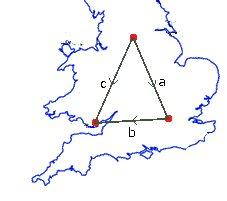
\includegraphics[scale=0.5]{uk.jpg}
  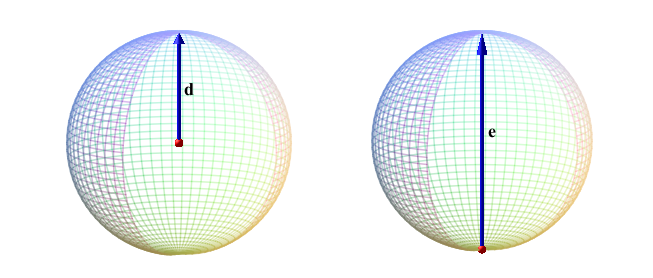
\includegraphics[scale=0.4]{globes.png}
 \end{center}
 Once we have agreed on where our axes should point, and
 what units of length we should use, we can identify $U$
 with $\R^3$.  However, it is conceptually important
 (especially in the theory of relativity) that $U$ exists in
 its own right without any such choice of conventions.
\end{example}

\begin{example}\lbl{eg-FR}
 The set $F(\R)$ of all functions from $\R$ to $\R$ is a
 vector space, because we can add any two functions to get a
 new function, and we can multiply a function by a number to
 get a new function.  For example, we can define functions
 $f,g,h\:\R\xra{}\R$ by
 \begin{align*}
   f(x) &= e^x \\
   g(x) &= e^{-x} \\
   h(x) &= \cosh(x) = (e^x + e^{-x})/2,
 \end{align*}
 so $f$, $g$ and $h$ are elements of $F(\R)$.  Then $f+g$
 and $2h$ are again functions, in other words $f+g\in F(\R)$
 and $2h\in F(\R)$.  Of course we actually have $f+g=2h$ in
 this example.

 For this to work properly, we must insist that $f(x)$ is
 defined for all $x$, and is a real number for all $x$; it
 cannot be infinite or imaginary.  Thus the rules $p(x)=1/x$
 and $q(x)=\sqrt{x}$ do not define elements $p,q\in F(\R)$.
\end{example}
\begin{remark}
 In order to understand the above example, you need to think
 of a function $f\:\R\to\R$ as a single object in its own
 right, and then think about the set $F(\R)$ of all possible
 functions as a single object; later you will need to think
 about various different subsets of $F(\R)$.  All this may
 seem quite difficult to deal with.  However, it is a
 \emph{central aim} of this course for you to get to grips
 with this level of abstraction.  So you should persevere,
 ask questions, study the notes and work through examples
 until it becomes clear to you.
\end{remark}

\begin{example}\lbl{eg-CR}
 In practise, we do not generally want to consider the set
 $F(\R)$ of \emph{all} functions.  Instead we consider the
 set $C(\R)$ of continuous functions, or the set
 $C^\infty(\R)$ of ``smooth'' functions (those which can be
 differentiated arbitrarily often), or the set $\R[x]$ of
 polynomial functions (eg $p(x)=1+x+x^2+x^3$ defines an
 element $p\in\R[x]$).  If $f$ and $g$ are continuous then
 $f+g$ and $tf$ are continuous, so $C(\R)$ is a vector
 space.  If $f$ and $g$ are smooth then $f+g$ and $tf$ are
 smooth, so $C^\infty(\R)$ is a vector space.  If $f$ and
 $g$ are polynomials then $f+g$ and $tf$ are polynomials, so
 $\R[x]$ is a vector space.
\end{example}

\begin{example}\lbl{eg-Cab}
 We also let $[a,b]$ denote the interval
 $\{x\in\R\st a\leq x\leq b\}$, and we write $C[a,b]$ for
 the set of continuous functions $f\:[a,b]\xra{}\R$.  For
 example, the rule $f(x)=1/x$ defines a continuous function
 on the interval $[1,2]$.  (The only potential problem is at
 the point $x=0$, but $0\not\in[1,2]$, so we do not need to
 worry about it.)  We thus have an element $f\in C[1,2]$.
\end{example}

\begin{example}\lbl{eg-matrices}
 The set $M_2\R$ of $2\tm 2$ matrices (with real entries) is
 a vector space.  Indeed, if we add two such matrices, we
 get another $2\tm 2$ matrix, for example
 \[ \bsm 1 & 0 \\ 0 & 4 \esm + \bsm 0 & 2 \\ 3 & 0 \esm =
     \bsm 1 & 2 \\ 3 & 4 \esm.
 \]
 Similarly, if we multiply a $2\tm 2$ matrix by a real
 number, we get another $2\tm 2$ matrix, for example
 \[ 7 \bsm 1 & 2 \\ 3 & 4 \esm = \bsm 7 & 14 \\ 21 & 28 \esm. \]
 We can identify $M_2\R$ with $\R^4$, by the rule
 \[ \bsm a & b \\ c & d \esm \leftrightarrow
     \bsm a \\ b \\ c \\ d \esm.
 \]

 More generally, for any $n$ the set $M_n\R$ of $n\tm n$
 square matrices is a vector space, which can be identified
 with $\R^{n^2}$.  More generally still, for any $n$ and
 $m$, the set $M_{n,m}\R$ of $n\tm m$ matrices is a vector
 space, which can be identified with $\R^{nm}$.
\end{example}


\begin{example}\lbl{eg-lists}
 Let $L$ be the set of all finite lists of real numbers.
 For example, the lists $\va=(10,20,30,40)$ and
 $\vb=(5,6,7)$ and $\vc=(1,\pi,\pi^2)$ define three elements
 $\va,\vb,\vc\in L$.  Is $L$ a vector space?  In trying to
 answer this question, we will reveal some inadequacies of
 Predefinition~\ref{predef-vector-space}. 

 It seems clear that $L$ is closed under scalar
 multiplication: for example $100\vb=(500,600,700)$, which
 is another element of $L$.  The real issue is closure under
 addition.  For example, is $\va+\vb$ an element of $L$?  We
 cannot answer this unless we know what $\va+\vb$ means.
 There are at least three possible meanings:
 \begin{itemize}
  \item[(1)] $\va+\vb$ could mean $(10,20,30,40,5,6,7)$ 
   (the list $\va$ followed by the list $\vc$).
  \item[(2)] $\va+\vb$ could mean $(15,26,37)$
   (chop off $\va$ to make the lists the same length, then
   add them together).
  \item[(3)] $\va+\vb$ could mean $(15,26,37,40)$ 
   (add zeros to the end of $\vc$ to make the lists the same
   length, then add them together.)
 \end{itemize}
 The point is that the expression $\va+\vb$ does not have a
 meaning until we decide to give it one.  (Strictly
 speaking, the same is true of the expression $100\vb$, but
 in that case there is only one reasonable possibility for
 what it should mean.)  To avoid this kind of ambiguity, we
 should say that a vector space is a set \emph{together with
  a definition of addition} etc.

 Suppose we agree to use the third definition of addition,
 so that $\va+\vb=(15,26,37,40)$.  The ordinary rules of
 algebra would tell us that $(\va + (-1).\va) + \vb=\vb$.
 However, in fact we have
 \begin{align*}
  (\va + (-1).\va) + \vb &=
   ((10,20,30,40) + (-10,-20,-30,-40)) + (5,6,7) \\
  &= (0,0,0,0) + (5,6,7) = (5,6,7,0) \\
  &\neq (5,6,7) = \vb.
 \end{align*}
 Thus, the ordinary rules of algebra do not hold.  We do not
 want to deal with this kind of thing; we only want to
 consider sets where addition and scalar multiplication work
 in the usual way.  We must therefore give a more careful
 definition of a vector space, which will allow us to say
 that $L$ is not a vector space, so we need not think about
 it. 

 (If we used either of the other definitions of addition
 then things would still go wrong; details are left as an
 exercise.) 
\end{example}
\begin{example}\lbl{eg-PR}
 Now consider the collection $W$ of all subsets of $\R$, so
 for example the sets $A=\{1,2\}$ and $B=\{30,40,50\}$ are
 elements of $W$.  We shall try to decide whether $W$ is a
 vector space, and in doing so, we will understand why our
 original definition is not satisfactory.  If $W$ is to be a
 vector space, then $2A$ and $A+B$ should be elements of
 $W$.  But what do $2A$ and $A+B$ actually mean?  It seems
 clear that $2A$ should mean $\{2,4\}$, but $A+B$ is less
 obvious.  One possible answer is that $A+B$ should just
 mean the union of $A$ and $B$, so
 \[ A+B = A\cup B = \{1,2,30,40,50\}. \]
 Another possible answer is that $A+B$ should mean the set
 of all sums $a+b$ with $a\in A$ and $b\in B$; this gives
 \[ A+B = \{1+30,1+40,1+50,2+30,2+40,2+50\} =
          \{31,32,41,42,51,52\}.
 \]
 To avoid this kind of ambiguity, we should say that a
 vector space is a set \emph{together with a definition of
  addition} etc.

 Suppose we agree on the second meaning of $A+B$.  By our
 original definition, we see that $W$ is a vector space: the
 sum of any two subsets of $\R$ is another subset of $\R$,
 and the product of a real number and a subset of $\R$ is
 again a subset of $\R$.  However, some funny things happen.
 For example, we have
 \[ A+10 A = \{1,2\} + \{10,20\} =
      \{1+10,1+20,2+10,2+20\} = \{11,12,21,22\}, 
 \]
 whereas $11A=\{11,22\}$, so $A+10A\neq 11A$.  We certainly
 don't want to allow this, so we should change the
 definition so that $W$ does not count as a vector space.
 (If we used the first definition of addition instead of the
 second one, then things would still go wrong.)
\end{example}

Our next attempt at a definition is as follows:
\begin{predefinition}\lbl{predef-vector-space-ii}
 A vector space over $\R$ is a nonempty set $V$, together
 with a definition of what it means to add elements of $V$
 or multiply them by real numbers, such that
 \begin{itemize}
  \item[(a)] If $u$ and $v$ are elements of $V$, then $u+v$ is an
   also an element of $V$.
  \item[(b)] If $u$ is an element of $V$ and $t$ is a real number, then
   $tu$ is an element of $V$.
  \item[(c)] All the usual algebraic rules for addition and
   multiplication hold.
 \end{itemize}
\end{predefinition}

In the course we will be content with an informal
understanding of the phrase ``all the usual algebraic
rules'', but for completeness, we give an explicit list of
axioms:
\begin{definition}\lbl{defn-real-vector-space}
 A vector space over $\R$ is a set $V$, together with an
 element $0\in V$ and a definition of what it means to add
 elements of $V$ or multiply them by real numbers, such that
 \begin{itemize} 
  \item[(a)] If $u$ and $v$ are elements of $V$, then $u+v$
   is an also an element of $V$.
  \item[(b)] If $v$ is an element of $V$ and $t$ is a real
   number, then $tv$ is an element of $V$.
  \item[(c)] For any elements $u,v,w\in V$ and any real
   numbers $s,t$, the following equations hold:
    \begin{enumerate}
     \item $0+v=v$
     \item $u+v=v+u$
     \item $u+(v+w)=(u+v)+w$
     \item $0u=0$
     \item $1u=u$
     \item $(st)u=s(tu)$
     \item $(s+t)u=su+tu$
     \item $s(u+v)=su+sv$.
    \end{enumerate}
 \end{itemize}  
\end{definition}
Note that there are many rules that do not appear explicitly
in the above list, such as the fact that
$t(u+v-w/t)=tu+tv-w$, but it turns out that all such rules
can be deduced from the ones listed.  We will not discuss
any such deductions.

In example~\ref{eg-lists}, the only element $0\in L$ with
the property that $0+v=v$ for all $v$ is the empty list
$0=()$.  If $u$ is a nonempty list of length $n$, then $0u$
is a list of $n$ zeros, which is not the same as the empty
list, so the axiom $0u=0$ is not satisfied, so $L$ is not a
vector space.  In all our other examples, it is obvious that
the axioms hold, and we will not discuss them further.

In example~\ref{eg-PR}, the fact that $A+10A\neq 11A$
contradicts the axiom $(s+t)u=su+tu$, so $W$ is not a vector
space.  (Some of the other axioms hold, and some of them do
not; we leave the details as an exercise.)  In all our other
examples, it is obvious that the axioms hold, and we will
not discuss them further.

\begin{remark}\lbl{rem-zero-notation}
 We will usually use the symbol $0$ for the zero element of
 whatever vector space we are considering.  Thus $0$ could
 mean the vector $\bsm 0\\0\\0\esm$ (if we are working with
 $\R^3$) or the zero matrix $\bsm 0&0&0\\0&0&0\esm$ (if we
 are working with $M_{2,3}\R$) or whatever.  Occasionally it
 will be important to distinguish between the zero elements
 in different vector spaces.  In that case, we write $0_V$
 for the zero element of $V$.  For example, we have
 $0_{\R^2}=\bsm 0\\0\esm$ and $0_{M_2\R}=\bsm 0&0\\0&0\esm$.
\end{remark}

One can also consider vector spaces over fields other than
$\R$; the most important case for us will be the field $\C$
of complex numbers.  We record the definitions for
completeness. 
\begin{definition}\lbl{defn-field}
 A \emph{field} is a set $K$ together with elements
 $0,1\in K$ and a definition of what it means to add or
 multiply two elements of $K$, such that:
 \begin{enumerate}
  \item[(a)] The usual rules of algebra are valid.  More
   explicitly, for all $a,b,c\in K$ the following equations
   hold: 
   \begin{itemize}
    \item $0+a=a$
    \item $a+(b+c)=(a+b)+c$
    \item $a+b=b+a$
    \item $1.a=a$
    \item $a(bc)=(ab)c$
    \item $ab=ba$
    \item $a(b+c)=ab+ac$
   \end{itemize}
  \item[(b)] For every $a\in K$ there is an element $-a$ with
   $a+(-a)=0$.
  \item[(c)] For every $a\in K$ with $a\neq 0$ there is an
   element $a^{-1}\in K$ with $aa^{-1}=1$.
  \item[(d)] $1\neq 0$.
 \end{enumerate}
\end{definition}
\begin{example}\lbl{eg-fields}
 Recall that 
 \begin{align*}
  \Z &= \{ \text{ integers } \} =
        \{ \dotsc,-2,-1,0,1,2,3,4,\dotsc \} \\
  \Q &= \{ \text{ rational numbers } \} =
        \{ a/b\st a,b\in\Z\;,\; b\neq 0\} \\
  \R &= \{ \text{ real numbers } \} \\
  \C &= \{ \text{ complex numbers } \} = 
        \{ x+iy\st x,y\in\R \},
 \end{align*}
 so $\Z\subset\Q\subset\R\subset\C$.  Then $\R$, $\C$ and
 $\Q$ are fields.  The ring $\Z$ is not a field, because
 axiom~(c) is not satisfied: there is no element $2^{-1}$
 \emph{in the set $\Z$} for which $2.2^{-1}=1$.  One can
 show that the ring $\Z/n\Z$ is a field if and only if $n$
 is a prime number.
\end{example}

\begin{definition}\lbl{defn-vector-space}
 A vector space over a field $K$ is a set $V$, together with
 an element $0\in V$ and a definition of what it means to
 add elements of $V$ or multiply them by elements of $K$,
 such that
 \begin{itemize}
  \item[(a)] If $u$ and $v$ are elements of $V$, then $u+v$ is an
   also an element of $V$.
  \item[(b)] If $v$ is an element of $V$ and $t$ is an
   element of $K$, then $tv$ is an element of $V$.
  \item[(c)] For any elements $u,v,w\in V$ and any elements
   $s,t\in K$, the following equations hold:
    \begin{enumerate}
     \item $0+v=v$
     \item $u+v=v+u$
     \item $u+(v+w)=(u+v)+w$
     \item $0u=0$
     \item $1u=u$
     \item $(st)u=s(tu)$
     \item $(s+t)u=su+tu$
     \item $s(u+v)=su+sv$.
    \end{enumerate}
 \end{itemize}  
\end{definition}
\begin{example}\lbl{eg-other-fields}
 Almost all our examples of real vector spaces work over any
 field $K$.  For example, the set $M_4\Q$ (of $4\tm 4$
 matrices whose entries are rational numbers) is a vector
 space over $\Q$.  The set $\C[x]$ (of polynomials with
 complex coefficients) is a vector space over $\C$.
\end{example}


%============================================================
%============================================================

\begin{center}
 \Large \textbf{Exercises}
\end{center}

\begin{exercise}\exlabel{ex-typical-elements}
 For each of the following vector spaces $V$, write down two
 typical elements of $V$ (say $u$ and $v$), calculate $u+v$
 and $10v$, and observe that these are again elements of
 $V$.  (For example, in the case $V=\R^2$ we could take
 $u=\bsm 1\\2\esm$ and $v=\bsm 3\\4\esm$, then we would have
 $u+v=\bsm 4\\6\esm$ and $10v=\bsm 30\\40\esm$, both of
 which are again elements of $\R^2$.)
 \begin{center}
  (a)~~$V=\R^4$  \hspace{3em}
  (b)~~$V=M_{2,3}(\R)$ \hspace{3em}
  (c)~~$V=\R[x]$ \\
  (d) $V$ is the set of physical vectors, as in
   Example~2.6 in the notes.
 \end{center}
\end{exercise}
\begin{solution}
 Of course there are many different correct answers to this
 question. The following will do:
 \begin{itemize}
  \item[(a)] $u=\bsm 1\\1\\1\\1\esm$,
             $v=\bsm 1\\-1\\1\\-1\esm$,
             $u+v=\bsm 2\\0\\2\\0\esm$,
             $10v=\bsm 10\\-10\\10\\-10\esm$.
  \item[(b)] $u=\bsm 1&2&3\\4&5&6\esm$,
             $v=\bsm 6&5&4\\3&2&1\esm$,
             $u+v=\bsm 7&7&7\\7&7&7\esm$,
             $10v=\bsm 60&50&40\\30&20&10\esm$.
  \item[(c)] $u=1+x$, $v=x+x^2$, $u+v=1+2x+x^2$, $10v=10x+10x^2$. 
  \item[(d)] $u$ is the vector pointing 10 miles east, $v$
   is the vector pointing 20 miles west, $u+v$ points ten
   miles west, $10v$ points 200 miles west.
 \end{itemize}
\end{solution}
%------------------------------------------------------------

\begin{exercise}\exlabel{ex-not-vector-spaces}
 Explain why none of the following is a vector space (with
 the obvious definition of addition and scalar
 multiplication). 
 \begin{itemize}
  \item[(a)] $V_0=\left\{\bsm a&b\\ c&d\esm\in M_2\R\st a\leq b\leq
    c\leq d\right\}$
  \item[(b)] $V_1=\left\{\bsm a\\ b\esm\in\R^2\st
                         a+b\text{ is an odd integer } \right\}$
  \item[(c)] $V_2=\left\{\bsm x\\ y\esm\in\R^2 \st x^2=y^2\right\}$.
  \item[(d)] $V_3=\{p\in\R[x]\st p(0)p(1)=0\}$
 \end{itemize}
\end{exercise}
\begin{solution}
 \begin{itemize}
 \item[(a)] This is not a vector space because
  $\bsm 1&2\\3&4\esm\in V_0$ but 
  $(-1).\bsm 1&2\\3&4\esm=\bsm -1&-2\\-3&-4\esm\not\in V_0$,
  which contradicts axiom~(b) of Predefinition~2.1.
 \item[(b)] This is not a vector space because the zero matrix does
  not lie in $V_1$.
 \item[(c)] This is not a vector space because
  $\bsm 1\\1\esm\in V_2$ and $\bsm 1\\-1\esm\in V_2$
  but $\bsm 1\\1\esm+\bsm 1\\-1\esm=\bsm 2\\0\esm\not\in V_2$,
  which contradicts axiom~(a).
 \item[(d)] To see that this is not a vector space, consider
  the polynomials $p(x)=x$ and $q(x)=1-x$.  Then
  $p(0)p(1)=0=q(0)q(1)$, so $p\in V_3$ and $q\in V_3$.
  However, $p(x)+q(x)=1$ for all $x$, so $p+q\not\in V_3$.
  This contradicts axiom~(a).
 \end{itemize}
\end{solution}
%------------------------------------------------------------

\section{Linear maps}
\label{sec-linear}

\begin{definition}\lbl{defn-linear}
 Let $V$ and $W$ be vector spaces, and let $\phi\:V\xra{}W$ be a
 function (so for each element $v\in V$ we have an element
 $\phi(v)\in W$).  We say that $\phi$ is \emph{linear} if 
 \begin{itemize}
  \item[(a)] For any $v$ and $v'$ in $V$, we have
   $\phi(v+v')=\phi(v)+\phi(v')$ in $W$.
  \item[(b)] For any $t\in\R$ and $v\in V$ we have
   $\phi(tv)=t\phi(v)$ in $W$. 
 \end{itemize}
 By taking $t=v=0$ in~(b), we see that a linear map must satisfy
 $\phi(0)=0$.  Further simple arguments also show that
 $\phi(v-v')=\phi(v)-\phi(v')$.
\end{definition}
\begin{remark}\lbl{rem-linear-condensed}
 The definition can be reformulated slightly as follows.  A
 map $\phi\:V\to W$ is linear iff
 \begin{itemize}
  \item[(c)] For any $t,t'\in\R$ and any $v,v'\in V$ we have
   $\phi(tv+t'v')=t\phi(v)+t'\phi(v')$. 
 \end{itemize}
 To show that this reformulation is valid, we must show that
 if~(c) holds, then so do~(a) and~(b); and conversely,
 if~(a) and~(b) hold, then so does~(c).

 Condition~(a) is the special case of~(c) where $t=t'=1$, and
 condition~(b) is the special case where $t'=0$ and $v'=0$.
 Thus, if~(c) holds then so do~(a) and~(b).  Conversely,
 suppose that~(a) and~(b) hold, and that we have $t,t'\in\R$
 and $v,v'\in V$.  Condition~(a) tells us that
 $\phi(tv+t'v')=\phi(tv)+\phi(t'v')$, and condition~(b) tells
 us that $\phi(tv)=t\phi(v)$ and $\phi(t'v')=t'\phi(v')$.
 Putting these together, we get
 \[ \phi(tv+t'v')=t\phi(v)+t'\phi(v'), \]
 so condition~(c) holds, as required.
\end{remark}

\begin{example}\lbl{eg-square-nonlinear}
  Consider the functions $f,g\:\R\xra{}\R$ given by $f(x)=2x$ and
  $g(x)=x^2$.  Then
  \[ g(x+x') = x^2 + x'^2 + 2xx' \neq x^2 + x'^2 = g(x) + g(x'), \]
  so $g$ is not linear.  Similarly, for general $x$ and $x'$
  we have $\sin(x+x')\neq\sin(x)+\sin(x')$ and
  $\exp(x+x')\neq\exp(x)+\exp(x')$, so the functions $\sin$
  and $\exp$ are not linear.  On the other hand, we have
  \begin{align*}
    f(x+x') &= 2(x+x') = 2x + 2x' = f(x) + f(x') \\
    f(tx) &= 2tx = t f(x) 
  \end{align*}
  so $f$ is linear.
\end{example}

\begin{example}\lbl{eg-LRR}
 The obvious generalisation of the previous example is as
 follows.  For any number $m\in\R$, we can define
 $\mu_m\:\R\xra{}\R$ by $\mu_m(x)=mx$ (so $f$ in the
 previous example is $\mu_2$).  We have
 \begin{align*}
   \mu_m(x+x') &= m(x+x') = mx+mx' = \mu_m(x) + \mu_m(x') \\
   \mu_m(tx)   &= mtx = tmx = t\mu_m(x),
 \end{align*}
 so $\mu_m$ is linear (and in fact, these are all the linear
 maps from $\R$ to $\R$).  Note also that the graph of
 $\mu_m$ is a straight line of slope $m$ through the origin;
 this is essentially the reason for the word ``linear''.
\end{example}

\begin{example}\lbl{eg-rot-linear}
 For any $\vv\in\R^2$, we let $\rho(\vv)$ be the vector obtained
 by rotating $\vv$ through $90$ degrees anticlockwise around
 the origin.  It is well-known that the formula for this is
 $\rho\bsm x\\ y\esm=\bsm -y\\ x\esm$.
 \begin{center}
  \begin{tikzpicture}[scale=3] % [50]{-0.5}{1.5}{-0.5}{1.5}
   \draw[->] (-0.5,0) -- (1.5,0);
   \draw[->] (0,-0.5) -- (0,1.5);
   \draw (0,0) -- (0.8,0.6);
   \draw (0,0) -- (-0.6,0.8);
   \fill ( 0.0,0.0) circle(0.02);
   \fill ( 0.8,0.6) circle(0.02);
   \fill (-0.6,0.8) circle(0.02);
   \draw[dotted] (0.8,0.6) -- (0.8,0);
   \draw[dotted] (-0.6,0.8) -- (0,0.8);
   \draw (1,0.67) node {$\scriptstyle{x}$};
   \draw (1,0.53) node {$\scriptstyle{y}$};
   \draw[thick] (0.95,0.47) -- (0.92,0.47) -- (0.92,0.73) -- (0.95,0.73);
   \draw[thick] (1.05,0.47) -- (1.07,0.47) -- (1.07,0.73) -- (1.05,0.73);
   \draw (-0.85,0.87) node {$\scriptstyle{-y}$};
   \draw (-0.85,0.73) node {$\scriptstyle{x}$};
   \draw[thick] (-0.94,0.67) -- (-0.97,0.67) -- (-0.97,0.93) -- (-0.94,0.93);
   \draw[thick] (-0.70,0.67) -- (-0.67,0.67) -- (-0.67,0.93) -- (-0.70,0.93);
   \draw[ultra thick,red,->] (0,0) +(37:0.25) arc(37:127:0.25);
  \end{tikzpicture}
 \end{center}
 We thus have
 \begin{align*}
  \rho\left(\bsm \xx\\\yy\esm+\bsm x'\\ y'\esm\right) &=
   \rho\bsm \xx+x'\\ \yy+y'\esm =
       \bsm -\yy-y'\\ \xx+x'\esm =
       \bsm -\yy\\ \xx\esm + \bsm -y'\\ x'\esm = 
       \rho\bsm \xx\\ \yy\esm + \rho\bsm x'\\ y'\esm \\
  \rho\left(t\bsm \xx\\ \yy\esm\right) &=
    \rho\bsm t\xx\\ t\yy\esm =
    \bsm -t\yy \\ t\xx\esm = 
    t\rho\bsm \xx\\ \yy\esm,
 \end{align*}
 so $\rho$ is linear.  (Can you explain this geometrically,
 without using the formula?)
\end{example}

\begin{example}\lbl{eg-ref-linear}
 For any $\vv\in\R^2$, we let $\tau(\vv)$ be the vector
 obtained by reflecting $\vv$ across the line $y=0$.  It is
 clear that the formula is
 $\tau\bsm x\\ y\esm=\bsm x\\-y\esm$, and using this we see
 that $\tau$ is linear.
\begin{center}
  \begin{tikzpicture}[scale=3] % [50]{-0.5}{1.5}{-0.8}{0.8}
   \draw[->] (-0.5,0) -- (1.5,0);
   \draw[->] (0,-0.8) -- (0,0.8);
   \draw (0,0) -- (0.8,0.6);
   \draw (0,0) -- (0.8,-0.6);
   \fill ( 0.0, 0.0) circle(0.02);
   \fill ( 0.8, 0.6) circle(0.02);
   \fill ( 0.8,-0.6) circle(0.02);
   \draw[dotted] (0.8,0.6) -- (0.8,-0.6);
   \draw (1,0.67) node {$\scriptstyle{x}$};
   \draw (1,0.53) node {$\scriptstyle{y}$};
   \draw[thick] (0.95,0.47) -- (0.92,0.47) -- (0.92,0.73) -- (0.95,0.73);
   \draw[thick] (1.05,0.47) -- (1.07,0.47) -- (1.07,0.73) -- (1.05,0.73);
   \draw (1.04,-0.53) node {$\scriptstyle{x}$};
   \draw (1.04,-0.67) node {$\scriptstyle{-y}$};
   \draw[thick] (0.95,-0.47) -- (0.92,-0.47) -- (0.92,-0.73) -- (0.95,-0.73);
   \draw[thick] (1.15,-0.47) -- (1.17,-0.47) -- (1.17,-0.73) -- (1.15,-0.73);
   \draw[ultra thick,red,<->] (0.9,0.25) -- (0.9,-0.25);
  \end{tikzpicture}
 \end{center}
\end{example}

\begin{example}\lbl{eg-norm-nonlinear}
 Define $\tht\:\R^2\xra{}\R$ by $\tht(\vv)=\|\vv\|$, so
 $\tht\bsm x\\ y\esm=\sqrt{x^2+y^2}$.  This is not linear,
 because $\tht(\vu+\vv)\neq\tht(\vu)+\tht(\vv)$ in general.
 Indeed, if $\vu=\bsm 1\\0\esm$ and $\vv=\bsm -1\\0\esm$
 then $\tht(\vu+\vv)=0$ but $\tht(\vu)+\tht(\vv)=1+1=2$.
\end{example}

\begin{example}\lbl{eg-shift-nonlinear}
 Define $\sg\:\R^2\xra{}\R^2$ by
 $\sg\bsm x\\ y\esm=\bsm x+1\\ y-1\esm$.  Then
 $\sg$ is not linear, because
 $\sg\bsm 0\\0\esm\neq\bsm 0\\0\esm$.
\end{example}

\begin{example}\lbl{eg-homogeneous-nonlinear}
 Define $\al\:\R^2\to\R^2$ by 
 \[ \al\bsm x \\ y\esm =
     \bsm y^3/(x^2+y^2) \\ x^3/(x^2+y^2) \esm.
 \]
 (This does not really make sense when $x=y=0$, but for that
 case we make the separate definition that
 $\al\bsm 0\\0\esm=\bsm 0\\0\esm$.)  This map satisfies
 $\al(t\vv)=t\al(\vv)$, but it does not satisfy
 $\al(\vu+\vv)=\al(\vu)+\al(\vv)$, so it is not linear.  For
 example, if $\vu=\bsm 1\\0\esm$ and $\vv=\bsm 0\\1\esm$
 then $\al(\vu)=\vv$ and $\al(\vv)=\vu$ but
 $\al(\vu+\vv)=(\vu+\vv)/2\neq\al(\vu)+\al(\vv)$.
\end{example}

\begin{example}\lbl{eg-vector-algebra}
 Given vectors $\vu=\bsm u_1\\ u_2\\ u_3\esm$ and
 $\vv=\bsm v_1\\ v_2\\ v_3\esm$ in $\R^3$, recall that the
 inner product and cross product are defined by 
 \begin{align*}
  \ip{\vu,\vv} &= \vu . \vv = u_1v_1 + u_2v_2 + u_3v_3 \\
  \vu\tm\vv &= \bsm u_2 v_3 - u_3 v_2 \\
                    u_3 v_1 - u_1 v_3 \\
                    u_1 v_2 - u_2 v_1 \esm.
 \end{align*}
 Fix a vector $\va\in\R^3$.  Define $\al\:\R^3\xra{}\R$ by
 $\al(\vv)=\ip{\va,\vv}$ and $\bt\:\R^3\xra{}\R^3$ by
 $\bt(\vv)=\va\tm\vv$.  Then both $\al$ and $\bt$ are
 linear.  To prove this we must show that
 $\al(t\vv)=t\al(\vv)$ and $\al(\vv+\vw)=\al(\vv)+\al(\vw)$
 and $\bt(t\vv)=t\bt(\vv)$ and
 $\bt(\vv+\vw)=\bt(\vv)+\bt(\vw)$.  We will write out only
 the last of these; the others are similar but easier.
 \[ 
  \bt(\vv+\vw) = 
  \bt\bsm v_1+w_1 \\ v_2+w_2 \\ v_3+w_3 \esm = 
  \bsm a_2(v_3+w_3) - a_3(v_2+w_2) \\
       a_3(v_1+w_1) - a_1(v_3+w_3) \\
       a_1(v_2+w_2) - a_2(v_1+w_1) \esm = 
  \bsm a_2 v_3 - a_3 v_2 \\
       a_3 v_1 - a_1 v_3 \\
       a_1 v_2 - a_2 v_1 \esm +
  \bsm a_2 w_3 - a_3 w_2 \\
       a_3 w_1 - a_1 w_3 \\
       a_1 w_2 - a_2 w_1 \esm =
  \bt(\vv) + \bt(\vw).
 \]
\end{example}

\begin{example}\lbl{eg-matrix-linear}
 Let $A$ be a fixed $m\tm n$ matrix.  Given a vector $\vv$
 of length $n$ (so $\vv\in\R^n$), we can multiply $A$ by
 $\vv$ in the usual way to get a vector $A\vv$ of length
 $m$.  We can thus define $\phi_A\:\R^n\xra{}\R^m$ by
 $\phi_A(\vv)=A\vv$.  It is clear that
 $A(\vv+\vv')=A\vv+A\vv'$ and $At\vv=tA\vv$, so $\phi_A$ is
 a linear map.  We will see later that every linear map from
 $\R^n$ to $\R^m$ has this form.  In particular, if we put
 \[ R = \bsm 0 & -1 \\ 1 & 0 \esm \hspace{5em} 
    T = \bsm 1 & 0 \\ 0 & -1 \esm
 \] 
 we find that 
 \[ 
  R\bsm x \\ y\esm = \bsm -y\\ x\esm = 
   \rho\left(\bsm x\\ y\esm\right) \hspace{5em}
  T\bsm x \\ y\esm = \bsm x\\ -y\esm = 
   \tau\left(\bsm x\\ y\esm\right)
 \]
 (where $\rho$ and $\tau$ are as in
 Examples~\ref{eg-rot-linear} and~\ref{eg-ref-linear}).
 This means that $\rho=\phi_R$ and $\tau=\phi_T$.
\end{example}

\begin{example}\lbl{eg-int-linear}
 For any continuous function $f\:\R\xra{}\R$, we write
 \[ I(f) = \int_0^1f(x)dx \in \R. \]
 This defines a map $I\:C(\R)\xra{}\R$.  If we put
 \begin{align*}
   p(x) &= x^2 \\
   q(x) &= 2x-1 \\
   r(x) &= e^x
 \end{align*}
 we have $I(p)=1/3$ and $I(q)=0$ and $I(r)=e-1$.

 Using the obvious equations
 \begin{align*}
   \int_0^1 f(x)+g(x) dx &= \int_0^1 f(x)dx + \int_0^1 g(x) dx \\
   \int_0^1 t f(x) dx &= t \int_0^1 f(x) dx 
 \end{align*}
 we see that $I$ is a linear map.
\end{example}

\begin{definition}\lbl{eg-diff-linear}
 For any smooth function $f\:\R\xra{}\R$ we write $D(f)=f'$ and
 $L(f)=f''+f$.  These are again smooth functions, so we have maps
 $D\:C^\infty(\R)\xra{}C^\infty(\R)$ and
 $L\:C^\infty(\R)\xra{}C^\infty(\R)$.  If we put
 \begin{align*}
  p(x) &= \sin(x) \\
  q(x) &= \cos(x) \\
  r(x) &= e^x
 \end{align*}
 then $D(p)=q$ and $D(q)=-p$ and $D(r)=r$.  It follows that
 $L(p)=L(q)=0$ and that $L(r)=2r$.  Using the obvious equations
 \begin{align*}
  (f+g)' &= f' + g' \\
  (tf)'  &= t\;f'
 \end{align*}
 we see that $D$ is linear.  Similarly, we have
 \begin{align*}
  L(f+g) &= (f+g)'' + (f+g) 
          = f'' + g'' + f + g \\
         &= (f''+f) + (g''+g) 
          = L(f) + L(g) \\
  L(tf)  &= (tf)'' + tf 
          = t\; f'' + t f \\
         &= t L(f).
 \end{align*}
 This shows that $L$ is also linear.
\end{definition}

\begin{example}\lbl{eg-trace-det}
 For any $2\tm 2$ matrix $A=\bsm a & b\\ c & d\esm$, the
 trace and determinant are defined by $\trc(A)=a+d\in\R$
 and $\det(A)=ad-bc\in\R$.  We thus have two functions
 $\trc,\det\:M_2\R\xra{}\R$.  It is easy to see that
 $\trc(A+B)=\trc(A)+\trc(B)$ and
 $\trc(tA)=t\trc(A)$, so $\trc\:M_2\R\xra{}\R$ is a
 linear map.  On the other hand, we have
 $\det(tA)=t^2\det(A)$ and $\det(A+B)\neq\det(A)+\det(B)$ in
 general, so $\det\:M_2\R\xra{}\R$ is not a linear map.  For
 a specific counterexample, consider
 \[ A = \bsm 1 & 0 \\ 0 & 0 \esm 
    \hspace{3em} \text{ and } \hspace{3em}
    B = \bsm 0 & 0 \\ 0 & 1 \esm
 \]
 Then $\det(A)=\det(B)=0$ but $\det(A+B)=1$, so
 $\det(A+B)\neq\det(A)+\det(B)$.  

 None of this is really restricted to $2\tm 2$ matrices.
 For any $n$ we have a map $\trc\:M_n\R\xra{}\R$ given by
 $\trc(A)=\sum_{i=1}^nA_{ii}$, which is again linear.  We
 also have a determinant map $\det\:M_n\R\xra{}\R$ which
 satisfies $\det(tI)=t^n$; this shows that $\det$ is not
 linear, except in the silly case where $n=1$.
\end{example}

\begin{example}\lbl{eg-inv-nonlinear}
 ``Define'' $\phi\:M_2\R\xra{}M_2\R$ by $\phi(A)=A^{-1}$, so
 \[ \phi\bsm a & b \\ c & d\esm =
     \bsm d/(ad-bc) & -b/(ad-bc) \\ -c/(ad-bc) & a/(ad-bc) \esm. 
 \]
 This is not a linear map, simply because it is not a
 well-defined map at all: the ``definition'' does not make
 sense when $ad-bc=0$.  Even if it were well-defined, it
 would not be linear, because $\phi(I+I)=(2I)^{-1}=I/2$,
 whereas $\phi(I)+\phi(I)=2I$, so
 $\phi(I+I)\neq\phi(I)+\phi(I)$.
\end{example}

\pdfdest name{testdest} xyz

\begin{example}\lbl{eg-rref-nonlinear}
 Define $\phi\:M_3\R\xra{}M_3\R$ by 
 \[ \phi(A)=\text{ the row reduced echelon form of } A. \]
 For example, we have the following sequence of reductions:
 \[ \bsm 1&2&3 \\ 4&8&6 \\ 7&14&9 \esm \to
    \bsm 1&2&3 \\ 0&0&-6 \\ 0&0&-12 \esm \to
    \bsm 1&2&3 \\ 0&0&1 \\ 0&0&-12 \esm \to
    \bsm 1&2&0 \\ 0&0&1 \\ 0&0&0 \esm,
 \]
 which shows that
 \[ \phi\bsm 1&2&3 \\ 4&8&6 \\ 7&14&9 \esm  = 
    \bsm 1&2&0 \\ 0&0&1 \\ 0&0&0 \esm.
 \]
 The map is not linear, because $\phi(I)=I$ and also
 $\phi(2I)=I$, so $\phi(2I)\neq 2\phi(I)$.
\end{example}

\begin{example}\lbl{eg-transpose-linear}
 We can define a map $\trans\:M_n\R\xra{}M_n\R$ by $\trans(A)=A^T$.
 Here as usual, $A^T$ is the transpose of $A$, which is obtained by
 flipping $A$ across the main diagonal.  For example:
 \[ \bsm 1 & 2 & 3 \\ 0 & 4 & 5 \\ 0 & 0 & 6 \esm^T =
    \bsm 1 & 0 & 0 \\ 2 & 4 & 0 \\ 3 & 5 & 6 \esm.
 \]
 In general, we have $(A^T)_{ij}=A_{ji}$.  It is clear that 
 $(A+B)^T=A^T+B^T$ and $(tA)^T=tA^T$, so $\trans\:M_n\R\xra{}M_n\R$
 is a linear map.
\end{example}

\begin{definition}\lbl{defn-iso}
 We say that a linear map $\phi\:V\to W$ is an
 \emph{isomorphism} if it is a bijection, so there is an
 inverse map $\phi^{-1}\:W\xra{}V$ with
 $\phi(\phi^{-1}(w))=w$ for all $w\in W$, and
 $\phi^{-1}(\phi(v))=v$ for all $v\in V$.  (It turns out
 that $\phi^{-1}$ is automatically a \emph{linear} map - we
 leave this as an exercise.)  We say that $V$ and $W$ are
 \emph{isomorphic} if there exists an isomorphism from $V$
 to $W$.
\end{definition}
\begin{example}\lbl{eg-iso-matrices}
 We can now rephrase part of Example~\ref{eg-matrices} as
 follows: there is an isomorphism $\phi\:M_2\R\xra{}\R^4$
 given by $\phi\bsm a&b\\ c&d\esm=[a,b,c,d]^T$, so $M_2\R$ is
 isomorphic to $\R^4$.  Similarly, the space $M_{p,q}\R$ is
 isomorphic to $\R^{pq}$.
\end{example}
\begin{example}\lbl{eg-iso-physical}
 Let $U$ be the space of physical vectors, as in
 Example~\ref{eg-physical}.  A choice of axes and length
 units gives rise to an isomorphism from $\R^3$ to $U$.
 More explicitly, choose a point $P$ on the surface of the
 earth (for example, the base of the Eiffel Tower) and put
 \begin{align*}
  \vu &=
   \text{ the vector of length 1 km pointing east from $P$ } \\
  \vv &=
   \text{ the vector of length 1 km pointing north from $P$ } \\
  \vw &=
   \text{ the vector of length 1 km pointing vertically upwards from $P$. }
 \end{align*}
 Define $\phi\:\R^3\to U$ by $\phi(x,y,z)=x\vu+y\vv+z\vw$.
 Then $\phi$ is an isomorphism.
\end{example}
We will be able to give more interesting examples of
isomorphisms after we have learnt about subspaces.

%============================================================
%============================================================

\begin{center}
 \Large \textbf{Exercises}
\end{center}

\begin{exercise}\exlabel{ex-check-linear}
 Which of the following rules defines a linear map?
 \begin{itemize}
  \item[(a)] $\phi_0\:\R^2\to\R^2$ given by
   $\phi_0\bsm x\\ y\esm=\bsm x+y\\ x-y\esm$
  \item[(b)] $\phi_1\:\R^3\to\R$ given by 
   $\phi_1\bsm x\\ y\\ z\esm=xyz$
  \item[(c)] $\phi_2\:M_2\R\to\R$ given by
   $\phi_2\bsm a&b\\ c&d\esm=\max(|a|,|b|,|c|,|d|)$
  \item[(d)] $\phi_3\:\R[x]\to\R$ given by
   $\phi_3(f)=f(0)+f'(1)+f''(2)$
  \item[(e)] $\phi_4\:\R[x]\to\R$ given by
   $\phi_4(f)=f(0)f(1)$.  
 \end{itemize}
\end{exercise}
\begin{solution}
 The maps $\phi_0$ and $\phi_3$ are linear.  Indeed, we have
 \begin{align*}
  \phi_0\left(\bsm x\\ y\esm + \bsm x'\\ y'\esm\right) &=
  \phi_0\bsm x+x' \\ y+y' \esm = 
  \bsm (x+x')+(y+y') \\ (x+x')-(y+y') \esm \\
  &= \bsm x+y+x'+y' \\ x-y+x'-y' \esm = 
   \bsm x+y \\ x-y \esm + \bsm x'+y' \\ x'-y'\esm  \\
  &= \phi_0\bsm x\\ y\esm + \phi_0\bsm x'\\ y'\esm \\
  \phi_0\left(t\bsm x\\y\esm\right) &= 
   \phi_0\bsm tx\\ ty \esm = \bsm tx+ty\\ tx-ty\esm =
   t\bsm x+y\\ x-y\esm = t\phi_0\bsm x\\ y\esm \\
  \phi_3(f+g) &= 
   (f+g)(0) + (f+g)'(1) + (f+g)''(2) 
   = f(0) + g(0) + f'(1) + g'(1) + f''(2) + g''(2) \\
   &= (f(0)+f'(1)+f''(2)) + (g(0)+g'(1)+g''(2)) 
    = \phi_3(f) + \phi_3(g) \\
  \phi_3(tf) &= (tf)(0) + (tf)'(1) + (tf)''(2) 
    = t(f(0) + f'(1) + f''(2)) = t\phi_3(f).
 \end{align*}
 For the others:
 \begin{itemize}
  \item[(b)] Consider the vectors
   \[ \ve_1=\bsm 1\\0\\0 \esm \hspace{3em}
      \ve_2=\bsm 0\\1\\0 \esm \hspace{3em}
      \ve_3=\bsm 0\\0\\1 \esm.
   \]
   Then $\phi_1(\ve_1)=\phi_1(\ve_2)=\phi_1(\ve_3)=0$.  However,
   we have 
   \[ \phi_1(\ve_1+\ve_2+\ve_3) = \phi_1\bsm 1\\1\\1\esm =  1, \]
   so
   \[ \phi_1(\ve_1+\ve_2+\ve_3)\neq
       \phi_1(\ve_1)+\phi(\ve_2)+\phi(\ve_3),
   \]
   so $\phi_1$ is not linear.
  \item[(c)] We have $\phi_2(I)=1$ and $\phi_2((-1).I)=1$,
   so $\phi_2((-1).I)\neq(-1).\phi_2(I)$, so $\phi_2$ is not
   linear.
  \item[(e)] Consider the polynomials $p(x)=x$ and
   $q(x)=1-x$.  Then $\phi_4(p)=0\tm 1=0$ and
   $\phi_4(q)=1\tm 0=0$, but $\phi_4(p+q)=1\tm 1=1$, so
   $\phi_4(p+q)\neq\phi_4(p)+\phi_4(q)$, so $\phi_4$ is not
   linear. 
 \end{itemize}
\end{solution}
%------------------------------------------------------------

\begin{exercise}\exlabel{ex-find-eg-linear}
 In each of the cases below, give an example of a nonzero
 linear map $\phi\:V\to W$.  (Here ``nonzero'' means that
 there is at least one $v\in V$ such that $\phi(v)\neq 0$.)
 \begin{itemize}
  \item[(a)] $V=\R^4$ and $W=\R^2$
  \item[(b)] $V=M_3\R$ and $W=\R^2$
  \item[(c)] $V=M_3\R$ and $W=\R[x]$
  \item[(d)] $V=\R[x]$ and $W=M_2\R$
 \end{itemize}
\end{exercise}
\begin{solution}
 Of course there are many different correct answers for this
 question.  The following will do:
 \begin{itemize}
  \item[(a)] $\phi\bsm w\\ x\\ y\\ z\esm=\bsm w+x\\ y+z\esm$
  \item[(b)] $\phi\bsm a&b&c \\ d&e&f\\ g&h&i\esm = \bsm a\\ i\esm$
  \item[(c)] $\phi\bsm a&b&c \\ d&e&f\\ g&h&i\esm = ax^2+bx+c$
  \item[(d)] $\phi(f)=\bsm f(0) & 0 \\ 0 & f(1) \esm$.
 \end{itemize}
\end{solution}
%------------------------------------------------------------
\begin{exercise}\exlabel{ex-char-nonlinear}
 Define $\chi\:M_n\R\xra{}\R[t]_{\leq n}$ by
 \[ \chi(A) = \det(tI-A) =
      \text{ the characteristic polynomial of } A.
 \]
 Is this a linear map?
\end{exercise}
\begin{solution}
 No, because $\chi(0)=t^n\neq 0$, for example.
\end{solution}
%------------------------------------------------------------
\begin{exercise}\exlabel{ex-spectral-radius}
 Given a matrix $A\in M_n\C$, we write $\rho(A)$ for the
 \emph{spectral radius} of $A$, which is the largest
 absolute value of any eigenvalue of $A$.  In symbols, we
 have 
 \[ \rho(A) = \max\{|\lm| \st \det(\lm I - A)=0\}. \]
 Is $\rho\:M_n\C\to\C$ a linear map?
\end{exercise}
\begin{solution}
 No.  The eigenvalues of $\lm I$ are all equal to $\lm$, so
 $\rho(\lm I)=|\lm|$, whereas if $\rho$ were linear we would
 have to have $\rho(\lm I)=\lm\rho(I)=\lm$.  Alternatively,
 we have $\rho(I)=\rho(-I)=1$ but $\rho(0)=0$, so
 $\rho(I+(-I))\neq\rho(I)+\rho(-I)$.  
\end{solution}
%------------------------------------------------------------

\section{Subspaces}
\label{sec-subspaces}

\begin{definition}\lbl{defn-subspace}
 Let $V$ be a vector space.  A \emph{vector subspace} (or just
 \emph{subspace}) of $V$ is a subset $W\sse V$ such that
 \begin{itemize}
  \item[(a)] $0\in W$
  \item[(b)] Whenever $u$ and $v$ lie in $W$, the element $u+v$ also
   lies in $W$.  (In other words, $W$ is closed under addition.)
  \item[(c)] Whenever $u$ lies in $W$ and $t$ lies in $\R$, the
   element $tu$ also lies in $W$.  (In other words, $W$ is
   closed under scalar multiplication.)
 \end{itemize}
 These conditions mean that $W$ is itself a vector space.
\end{definition}
\begin{remark}\lbl{rem-restricted-ops}
 Strictly speaking, a vector space is a set \emph{together
  with a definition of addition and scalar multiplication}
 such that certain identities hold.  We should therefore
 specify that addition in $W$ is to be defined using the
 same rule as for $V$, and similarly for scalar
 multiplication. 
\end{remark}
\begin{remark}\lbl{rem-subspace-condensed}
 The definition can be reformulated slightly as follows: a
 set $W\sse V$ is a subspace iff
 \begin{itemize}
  \item[(a)] $0\in W$
  \item[(d)] Whenever $u,v\in W$ and $t,s\in\R$ we have
   $tu+sv\in W$.
 \end{itemize}

 To show that this reformulation is valid, we must check
 that if condition~(d) holds then so do~(b) and~(c); and
 conversely, that if~(b) and~(c) hold then so does~(d).

 In fact, conditions~(b) is the special cases of~(d)
 where $t=s=1$, and condition~(c) is the special case of~(d)
 where $v=0$; so if~(d) holds then so do~(b) and~(c).
 Conversely, suppose that~(b) and~(c) hold, and that
 $u,v\in W$ and $t,s\in\R$.  Then condition~(c) tells us
 that $tu\in W$, and similarly that $sv\in W$.  Given these,
 condition~(b) tells us that $tu+sv\in W$; we conclude that
 condition~(d) holds, as required.
\end{remark}

\begin{example}\lbl{eg-silly-subspaces}
 There are two silly examples: $\{0\}$ is always a subspace
 of $V$, and $V$ itself is always a subspace of $V$.
\end{example}

\begin{example}\lbl{eg-subspaces-R-two}
 Any straight line through the origin is a subspace of
 $\R^2$.  These are the only subspaces of $\R^2$ (except for
 the two silly examples).
\end{example}

\begin{example}\lbl{eg-subspaces-R-three}
 In $\R^3$, any straight line through the origin is a
 subspace, and any plane through the origin is also a
 subspace.  These are the only subspaces of $\R^3$ (except
 for the two silly examples).
\end{example}

\begin{example}\lbl{eg-trace-free}
 The set $W=\{A\in M_2\R\st\trc(A)=0\}$ is a subspace of
 $M_2\R$.  To check this, we first note that $0\in W$.  
 Suppose that $A,A'\in W$ and
 $t,t'\in\R$.  We then have $\trc(A)=\trc(A')=0$
 (because $A,A'\in W$) and so 
 \[ \trc(tA+t'A')=t \trc(A)+t' \trc(A') = t.0+t'.0=0,
 \] 
 so $tA+t'A'\in W$.  Thus, conditions~(a) and~(d) in
 Remark~\ref{rem-subspace-condensed} is satisfied, showing
 that $W$ is a subspace as claimed.
\end{example}

\begin{example}\lbl{eg-Rx-subspace}
 Recall that $\R[x]$ denotes the set of all polynomial
 functions in one variable (so the functions $p(x)=x+1$ and
 $q(x)=(x+1)^5-(x-1)^5$ and $r(x)=1+4x^4+8x^8$ define
 elements $p,q,r\in\R[x]$).  It is clear that the sum of two
 polynomials is another polynomial, and any polynomial
 multiplied by a constant is also a polynomial, so $\R[x]$
 is a subspace of the vector space $F(\R)$ of all functions on
 $\R$.

 We write $\R[x]_{\leq d}$ for the set of polynomials of
 degree at most $d$, so a general element $f\in\R[x]_{\leq
  d}$ has the form
 \[ f(x) =
     a_0 + a_1x + \ldots + a_d x^d = \sum_{i=0}^d a_ix^i
 \]
 for some $a_0,\ldots,a_d\in\R$.  It is easy to see that
 this is a subspace of $\R[x]$.
  
 If we let $f$ correspond to the vector
 $\bsm a_0&\dotsb&a_d\esm^T\in\R^{d+1}$, we get a one-to-one
 correspondence between $\R[x]_{\leq d}$ and $\R^{d+1}$.
 More precisely, there is an isomorphism
 $\phi\:\R^{d+1}\to\R[x]_{\leq d}$ given by 
 \[ \phi(\bsm a_0&\dotsb&a_d\esm^T) = 
     \sum_{i=0}^d a_i x^i.
 \]
\end{example}
\begin{remark}\lbl{rem-off-by-one}
 It is a common mistake to think that $\R[x]_{\leq d}$ is
 isomorphic to $\R^d$ (rather than $\R^{d+1}$), but this is
 not correct.  Note that the list $0,1,2,3$ has four entries
 (not three), and similarly, the list $0,1,2,\dotsc,d$ has
 $d+1$ entries (not $d$).
\end{remark}

\begin{example}\lbl{eg-even-odd}
 A function $f\:\R\xra{}\R$ is said to be \emph{even} if
 $f(-x)=f(x)$ for all $x$, and \emph{odd} if $f(-x)=-f(x)$
 for all $x$.  For example, $\cos(-x)=\cos(x)$ and
 $\sin(-x)=-\sin(x)$, so $\cos$ is even and $\sin$ is odd.
 (Of course, most functions are neither even nor odd.)
 We write $EF$ for the set of even functions, so $EF$ is a
 subset of the set $F(\R)$ of all functions from $\R$ to $\R$,
 and $\cos\in EF$.  If $f$ and $g$ are even, it is clear
 that $f+g$ is also even.  If $f$ is even and $t$ is a
 constant, then it is clear that $tf$ is also even; and the
 zero function is certainly even as well.  This shows that
 $EF$ is actually a subspace of $F(\R)$.  Similarly, the set
 $OF$ of odd functions is a subspace of $F(\R)$.
\end{example}


\begin{example}\lbl{eg-diffeq}
 Let $V$ be the vector space of smooth functions $u(x,t)$ in
 two variables $x$ and $t$ (to be thought of as position and
 time).
 \begin{itemize}
  \item We say that $u$ is a solution of the Wave Equation if
   \[ \frac{\partial^2 u}{\partial x^2} +
      \frac{\partial^2 u}{\partial t^2} = 0.
   \]
   This equation governs the propagation of small waves in deep
   water, or of electromagnetic waves in empty space.
  \item We say that $u$ is a solution of the Heat Equation if
   \[ \frac{\partial u}{\partial t} -
      \frac{\partial^2 u}{\partial x^2} = 0.
   \]
   This governs the flow of heat along an iron bar.
  \item We say that $u$ is a solution of the Korteweg-de Vries
   (KdV) equation  if
   \[ \frac{\partial u}{\partial t} + 
      \frac{\partial^3 u}{\partial x^3} -
      6 u\frac{\partial u}{\partial x} = 0.
   \]
   This equation governs the propagation of large waves in
   shallow water.
 \end{itemize}
 The set of solutions of the Wave Equation is a vector
 subspace of $V$, as is the set of solutions to the Heat
 Equation.  However, the sum of two solutions to the KdV
 equation does not satisfy the KdV equation, so the set of
 solutions is not a subspace of $V$.  In other words, the
 Wave Equation and the Heat Equation are linear, but the KdV
 equation is not.

 The distinction between linear and nonlinear differential
 equations is of fundamental importance in physics.  Linear
 equations can generally be solved analytically, or by
 efficient computer algorithms, but nonlinear equations
 require far more computing power.  The equations of
 electromagnetism are linear, which explains why hundreds of
 different radio, TV and mobile phone channels can coexist,
 together with visible light (which is also a form of
 electromagnetic radiation), with little or no interference.
 The motion of fluids and gasses is governed by the
 Navier-Stokes equation, which is nonlinear; because of
 this, massive supercomputers are needed for weather
 forecasting, climate modelling, and aircraft design.
\end{example}



\begin{example}\lbl{eg-matrix-subspaces}
 Consider the following sets of $3\tm 3$ matrices:
 \begin{align*}
   U_0 &= \{ \text{symmetric matrices} \} 
       &&= \{ A\in M_3\R \st A^T = A \} \\
   U_1 &= \{ \text{antisymmetric matrices} \}
       &&= \{ A\in M_3\R \st A^T = -A \} \\
   U_2 &= \{ \text{trace-free matrices} \} 
       &&= \{ A\in M_3\R \st \trc(A) = 0 \} \\
   U_3 &= \{ \text{ diagonal matrices } \} 
       &&= \{ A\in M_3\R \st A_{ij}=0 \text{ whenever } i\neq j\} \\
   U_4 &= \{ \text{ strictly upper-triangular matrices } \} 
       &&= \{ A\in M_3\R \st A_{ij}=0 \text{ whenever } i\geq j\} \\
   U_5 &= \{ \text{ invertible matrices } \} 
       &&= \{ A\in M_3\R \st \det(A) \neq 0 \} \\
   U_6 &= \{ \text{ noninvertible matrices } \} 
       &&= \{ A\in M_3\R \st \det(A) = 0 \}
 \end{align*}
 Then $U_0,\ldots,U_4$ are all subspaces of $M_3\R$.  We
 will prove this for $U_0$ and $U_4$; the other cases are
 similar.  Firstly, it is clear that the zero matrix has
 $0^T=0$, so $0\in U_0$.  Suppose that $A,B\in U_0$
 (so $A^T=A$ and $B^T=B$) and $s,t\in\R$.  Then 
 \[ (sA+tB)^T = sA^T+tB^T = sA + tB, \]
 so $sA+tB\in U_0$.  Using
 Remark~\ref{rem-subspace-condensed}, we conclude that $U_0$
 is a subspace.  Now consider $U_4$.  The elements of $U_4$
 are the matrices of the form
 \[ A = \bbm 0 & a_{12} & a_{13} \\
             0 & 0      & a_{23} \\
             0 & 0      & 0  \ebm
 \]
 In particular, the zero matrix is an element of $U_4$ (with
 $a_{12}=a_{13}=a_{23}=0$).  Now suppose that $A,B\in U_4$
 and $s,t\in\R$.  We have 
 \[ sA + tB = 
    s \bbm 0& a_{12}& a_{13}\\ 0 &0 & a_{23}\\0&0&0\ebm +
    t \bbm 0& b_{12}& b_{13}\\ 0 &0 & b_{23}\\0&0&0\ebm =
    \bbm 0 & s a_{12} + t b_{12} & s a_{13} + t b_{13} \\
         0 & 0                   & s a_{23} + t b_{23} \\
         0 & 0                   & 0 \ebm,
 \]
 which shows that $sA+tB$ is again strictly upper
 triangular, and so is an element of $U_4$.  Using
 Remark~\ref{rem-subspace-condensed} again, we conclude that
 $U_4$ is also a subspace.

 On the other hand, $U_5$ is not a subspace, because it does
 not contain the zero matrix.  Similarly, $U_6$ is not a
 subspace: if we put
 \[ A = \bsm 1&0&0\\0&0&0\\0&0&0 \esm 
    \hspace{5em} 
    B = \bsm 0&0&0\\0&1&0\\0&0&1 \esm 
 \]
 then $A,B\in U_6$ but $A+B=I\not\in U_6$.
\end{example}

\begin{definition}\lbl{defn-sum}
 Let $U$ be a vector space, and let $V$ and $W$ be subspaces of $U$.
 We put 
 \[ V+W = \{ u \in U \st u = v+w
            \text{ for some } v\in V \text{ and } w\in W \}.
 \]
\end{definition}

\begin{example}\lbl{eg-sum-easy}
 If $U=\R^3$ and
 \[ V = \{\bsm x\\ 0\\ 0\esm\st x\in\R\} \hspace{5em}
    W = \{\bsm 0\\ 0\\ z\esm\st z\in\R\}
 \]
 then
 \[ V+W = \{\bsm x\\ 0\\ z\esm\st x,z\in\R\} \]
\end{example}
\begin{example}\lbl{eg-sum-matrix}
 If $U=M_2\R$ and
 \[ V = \{\bsm a & b \\ 0 & 0\esm\st a,b\in\R\} \hspace{5em}
    W = \{\bsm 0 & b \\ 0 & d\esm\st b,d\in\R\}
 \]
 then
 \[ V+W = \{\bsm a & b \\ 0 & d \esm\st a,b,d\in\R\}. \]
 Indeed, any matrix of the form $A=\bsm a&b\\ 0&d\esm$ can be written
 as $A=\bsm a&b\\0&0\esm+\bsm 0&0\\0&d\esm$ with
 $\bsm a&b\\0&0\esm\in V$ and $\bsm 0&0\\0&d\esm\in W$, so
 $A\in V+W$.  Conversely, any $A\in V+W$ can be written as $A=B+C$
 with $B\in V$ and $C\in W$.  This means that $B$ has the form $B=\bsm
 a&b_1\\0&0\esm$ for some $a,b_1\in\R$ and $C$ has the form
 $C=\bsm 0&b_2\\0&d\esm$ for some $b_2,d\in\R$, so
 $A=\bsm a&b_1+b_2\\ 0&d\esm$, which lies in $V+W$.
\end{example}

\begin{proposition}\lbl{prop-meet-sum}
 Let $U$ be a vector space, and let $V$ and $W$ be subspaces
 of $U$.  Then both $V\cap W$ and $V+W$ are subspaces of
 $U$.
\end{proposition}
\begin{proof}
 We first consider $V\cap W$.  As $V$ is a subspace we have
 $0\in V$, and as $W$ is a subspace we have $0\in W$, so
 $0\in V\cap W$.  Next, suppose we have $x,x'\in V\cap W$.
 Then $x,x'\in V$ and $V$ is a subspace, so $x+x'\in V$.
 Similarly, we have $x,x'\in W$ and $W$ is a subspace so
 $x+x'\in W$.  This shows that $x+x'\in V\cap W$, so $V\cap W$
 is closed under addition.  Finally consider $x\in V\cap W$
 and $t\in\R$.  Then $x\in V$ and $V$ is a subspace so
 $tx\in V$.  Similarly $x\in W$ and $W$ is a subspace so
 $tx\in W$.  This shows that $tx\in V\cap W$, so $V\cap W$
 is closed under scalar multiplication, so $V\cap W$ is a
 subspace. 

 Now consider the space $V+W$.  We can write $0$ as $0+0$
 with $0\in V$ and $0\in W$, so $0\in V+W$.  Now suppose we
 have $x,x'\in V+W$.  As $x\in V+W$ we can find $v\in V$ and
 $w\in W$ such that $x=v+w$.  As $x'\in V+W$ we can also
 find $v'\in V$ and $w'\in W$ such that $x'=v'+w'$.  We then
 have $v+v'\in V$ (because $V$ is closed under addition) and
 $w+w'\in W$ (because $W$ is closed under addition).  We
 also have $x+x'=(v+v')+(w+w')$ with $v+v'\in V$ and
 $w+w'\in W$, so $x+x'\in V+W$.  This shows that $V+W$ is
 closed under addition.  Now suppose we have $t\in\R$.  Then
 $tv\in V$ (because $V$ is closed under scalar
 multiplication) and $tw\in W$  (because $W$ is closed under
 scalar multiplication).  We thus have $tx=tv+tw$ with
 $tv\in V$ and $tw\in W$, so $tx\in V+W$.  This shows that
 $V+W$ is also closed under scalar multiplication, so it is
 a subspace.
\end{proof}

\begin{example}\lbl{eg-intersect-planes}
 Take $U=\R^3$ and 
 \begin{align*}
  V &= \{[x,y,z]^T \st x+2y+3z = 0 \} \\
  W &= \{[x,y,z]^T \st 3x+2y+z = 0 \}.
 \end{align*}
 We claim that 
 \[ V\cap W= \{[x,-2x,x]^T \st x\in\R\}. \]
 and $V+W=\R^3$.  Indeed, a vector $[x,y,z]^T$ lies in
 $V\cap W$ iff we have $x+2y+3z=0$ and also $3x+2y+z=0$.  If
 we subtract these two equations and divide by two, we find
 that $z=x$.  If we feed this back into the first equation,
 we see that $y=-2x$.  Conversely, if $y=-2x$ and $z=x$ we
 see directly that both equations are satisfied.  It follows
 that $V\cap W= \{[x,-2x,x]^T \st t\in\R\}$ as claimed.  

 Next, consider an arbitrary vector $\vu=[x,y,z]\in\R^3$.
 Put 
 \[ \vv = \frac{1}{12} \bbm 12 x + 8 y + 4z  \\
                            3  x + 2 y +  z  \\
                            -6 x - 4 y - 2 z \ebm 
    \hspace{4em}
    \vw = \frac{1}{12} \bbm - 8 y - 4z  \\
                            - 3 x + 10 y -  z  \\
                              6 x + 4 y + 14 z \ebm,
 \]
 so $\vv+\vw=\vu$.  One can check that 
 \begin{align*}
  (12 x + 8 y + 4z) + 2(3  x + 2 y +  z) + 3(-6 x - 4 y - 2 z) &= 0 \\
  3(- 8 y - 4z) + 2(- 3 x + 10 y -  z) + (6 x + 4 y + 14 z) &= 0
 \end{align*}
 so $\vv\in V$ and $\vw\in W$.  This shows that
 $\vu\in V+W$, so $V+W=\R^3$.
\end{example}
\begin{example}\lbl{eg-intersect-poly}
 Take  
 \begin{align*}
  U &= \R[x]_{\leq 4} \\
  V &= \{ f\in U\st f(0) = f'(0) = 0 \} \\
  W &= \{ f\in U \st f(-x) = f(x) \text{ for all } x\}.
 \end{align*}
 To understand these, it is best to write the defining conditions more
 explicitly in terms of the coefficients of $f$.  Any element $f\in U$
 can be written as $f(x)=a_0+a_1x+a_2x^2+a_3x^3+a_4x^4$ for some
 $a_0,\dotsc,a_4$.  We then have
 \begin{align*}
  f(0) &= a_0 \\
  f'(x) &= a_1 + 2a_2x + 3a_3x^2 + 4a_4x^3 \\
  f'(0) &= a_1 \\
  f(-x) &= a_0-a_1x+a_2x^2-a_3x^3+a_4x^4 \\
  f(x)-f(-x) &= 2a_1x + 2a_3x^3 \\
 \end{align*}
 Thus $f\in V$ iff $a_0=a_1=0$, and $f\in W$ iff $f(x)=f(-x)$ iff
 $a_1=a_3=0$.  This means that 
 \begin{align*}
  U &= \{ a_0 + a_1x + a_2x^2 + a_3x^3 + a_4x^4 \st
          a_0,\dotsc,a_4\in\R \} \\
  V &= \{ a_2x^2 + a_3x^3 + a_4x^4 \st
          a_2,a_3,a_4\in\R \} \\
  W &= \{ a_0 + a_2x^2 + a_4x^4 \st
          a_0,a_2,a_4\in\R \}
 \end{align*}
 From this we see that $f\in V\cap W$ iff $a_0=a_1=a_3=0$, so
 \[ V\cap W = \{ a_2x^2 + a_4x^4 \st a_2,a_4\in\R\}. \]
 We next claim that $f\in V+W$ iff $a_1=0$, so $f$ has no term in
 $x^1$.  Indeed, from the formulae above we see that any polynomial in
 $V$ or in $W$ has no term in $x^1$, so if we add together a
 polynomial in $V$ and a polynomial in $W$ we will still have no term
 in $x^1$, so for $f\in V+W$ we have $a_1=0$ as claimed.  Conversely,
 if $f$ has no term in $x^1$ then we can write
 \[ f(x) = a_0+a_2x^2+a_3x^3+a_4x^4 = a_3x^3 + (a_0+a_2x^2+a_4x^4), \] 
 with $a_3x^3\in V$ and $a_0+a_2x^2+a_4x^4\in W$, so $f\in V+W$.

 In particular, the polynomial $f(x)=x$ does not lie in
 $V+W$, so $V+W\neq U$.
\end{example}

\begin{definition}\lbl{defn-ker-img}
 Let $U$ and $V$ be vector spaces, and let $\phi\:U\xra{}V$
 be a linear map.  Then the \emph{kernel} and \emph{image} of $\phi$
 are defined by
 \begin{align*}
   \ker(\phi) &=
    \{u\in U\st \phi(u) = 0 \} \\
   \img(\phi) &=
    \{v\in V \st v = \phi(u) \text{ for some } u\in U\}.
 \end{align*}
\end{definition}
\begin{example}\lbl{eg-ker-img-i}
 Define $\pi\:\R^3\to\R^3$ by
 $\pi\bsm x\\ y\\ z\esm=\bsm 0\\ y\\ z\esm$.  Then
 \begin{align*}
  \ker(\pi) &= \{\bsm x\\ 0\\ 0\esm\st x\in\R\} \\
  \img(\pi) &= \{\bsm 0\\ y\\ z\esm\st y,z\in\R\}
 \end{align*}
\end{example}

\begin{proposition}\lbl{prop-ker-img}
 Let $U$ and $V$ be vector spaces, and let $\phi\:U\xra{}V$ be a
 linear map.  Then $\ker(\phi)$ is a subspace of $U$, and
 $\img(\phi)$ is a subspace of $V$.
\end{proposition}
\begin{proof}
 Firstly, we have $\phi(0_U)=0_V$, which shows both that
 $0_U\in\ker(\phi)$ and that $0_V\in\img(\phi)$.  Next,
 suppose that $u,u'\in\ker(\phi)$, which means that
 $\phi(u)=\phi(u')=0$.  As $\phi$ is linear this implies
 that $\phi(u+u')=\phi(u)+\phi(u')=0+0=0$, so
 $u+u'\in\ker(\phi)$.  This shows that $\ker(\phi)$ is
 closed under addition.  Now suppose we have $t\in\R$.
 Using the linearity of $\phi$ again, we have
 $\phi(tu)=t\phi(u)=t.0=0$, so $tu\in\ker(\phi)$.  This
 means that $\ker(\phi)$ is also closed under scalar
 multiplication, so it is a subspace of $U$.  Now suppose we
 have $v,v'\in\img(\phi)$.  This means that we can find
 $x,x'\in U$ with $\phi(x)=v$ and $\phi(x')=v'$.  We thus
 have $x+x',tx\in U$ and as $\phi$ is linear we have
 $\phi(x+x')=\phi(x)+\phi(x')=v+v'$ and
 $\phi(tx)=t\phi(x)=tv$.  This shows that $v+v'$ and $tv$
 lie in $\img(\phi)$, so $\img(\phi)$ is closed under
 addition and scalar multiplication, so it is a subspace. 
\end{proof}

\begin{example}\lbl{eg-ker-img-ii}
 Define $\phi\:\R^3\xra{}\R^3$ by
 $\phi([x,y,z]^T)=[x-y,y-z,z-x]^T$.  Then 
 \begin{align*}
  \ker(\phi) &=
    \{[x,y,z]^T\in\R^3\st x=y=z\} =
    \{[t,t,t]^T\st t\in\R\} \\
  \img(\phi) &= 
    \{[x,y,z]^T\in\R^3\st x+y+z=0\} =
    \{[x,y,-x-y]^T\st x,y\in\R^2\}.
 \end{align*}
 Indeed, for the kernel we have $[x,y,z]^T\in\ker(\phi)$ iff
 $\phi([x,y,z]^T)=[0,0,0]^T$ iff $x-y=y-z=z-x=0$ iff $x=y=z$, which
 means that $[x,y,z]^T=[t,t,t]^T$ for some $t$.

 For the image, note that if $x+y+z=0$ then
 \[ \phi([0,-x,-x-y]^T) = [0-(-x),(-x)-(-x-y),-x-y-0]^T = 
     [x,y,z]^T,
 \]
 so $[x,y,z]^T\in\img(\phi)$.  Conversely, if $[x,y,z]^T\in\img(\phi)$
 then $[x,y,z]^T=\phi([u,v,w]^T)$ for some $u,v,w\in\R$, which means
 that $x=u-v$ and $y=v-w$ and $z=w-u$, so 
 \[ x+y+z = (u-v)+(v-w)+(w-u) = 0. \]
 Thus $\ker(\phi)$ is a line through the origin (and thus a
 one-dimensional subspace) and $\img(\phi)$ is a plane
 through the origin (and thus a two-dimensional subspace).
\end{example}

\begin{example}\lbl{eg-anti-symm}
 Define $\phi\:M_n\R\xra{}M_n\R$ by $\phi(A)=A-A^T$ (which
 is linear).  Then clearly $\phi(A)=0$ iff $A=A^T$ iff $A$
 is a symmetric matrix.  Thus 
 \[ \ker(\phi)=\{n\tm n \text{ symmetric matrices }\}. \]
 We claim that also 
 \[ \img(\phi)=\{n\tm n \text{ antisymmetric matrices }\}. \]
 For brevity, we write $W$ for the set of antisymmetric
 matrices, so we must show that $\img(\phi)=W$.  For any $A$
 we have $\phi(A)^T=(A-A^T)^T=A^T-A^{TT}$, but $A^{TT}=A$, so
 $\phi(A)^T=A^T-A=-\phi(A)$.  This shows that $\phi(A)$ is
 always antisymmetric, so $\img(\phi)\sse W$.  Next, if $B$
 is antisymmetric then $B^T=-B$ so
 $\phi(B/2)=B/2-B^T/2=B/2+B/2=B$.  Thus $B$ is
 $\phi(\text{something})$, so $B\in\img(\phi)$.  This shows
 that $W\sse\img(\phi)$, so $W=\img(\phi)$ as claimed.  
\end{example}

\begin{example}\lbl{eg-ker-img-iv}
 Define $\phi\:\R[x]_{\leq 1}\to\R^3$ by $\phi(f)=[f(0),f(1),f(2)]^T$.
 More explicitly, we have 
 \[ \phi(ax+b) = [b,a+b,2a+b]^T = a [0,1,2]^T + b [1,1,1]^T. \]
 If $ax+b\in\ker(\phi)$ then we must have $\phi(ax+b)=0$, or in other
 words $b=a+b=2a+b=0$, which implies that $a=b=0$ and so $ax+b=0$.
 This means that $\ker(\phi)=\{0\}$.  

 Next, we claim that 
 \[ \img(\phi) = \{[u,v,w]^T \st u-2v+w = 0\}. \]
 Indeed, if $[u,v,w]^T\in\img(\phi)$ then we must have
 $[u,v,w]=\phi(ax+b)=[b,a+b,2a+b]$ for some $a,b\in\R$.  This means
 that $u-2v+w=b-2(a+b)+2a+b=0$, as required.  Conversely, suppose that
 we have a vector $[u,v,w]^T\in\R^3$ with $u-2v+w=0$.  We then have
 $w=2v-u$ and so 
 \[ \phi((v-u)x+u) = 
     \bsm u \\ (v-u) + u \\ 2(v-u) + u \esm = 
     \bsm u \\ v \\ 2v-u \esm = 
     \bsm u \\ v \\ w \esm,
 \]
 so $[u,v,w]^T$ is in the image of $\phi$.
\end{example}
\begin{remark}\lbl{rem-ker-img-iv}
 How did we arrive at our description of the image, and our proof that
 that description is correct?  We need to consider a vector
 $[u,v,w]^T$ and ask whether it can be written as $\phi(f)$ for
 some polynomial $f(x)=ax+b$.  In other words, we want to have
 $[u,v,w]^T=[b,a+b,2a+b]^T$, which means that $u=b$ and $v=a+b$ and
 $w=2a+b$.  The first two equations tell us that the only possible
 solution is to take $a=v-u$ and $b=u$, so $f(x)=(v-u)x+u$.  This
 potential solution is only a real solution if the third equation
 $w=2a+b$ is also satisfied, which means that $w=2(v-u)+u=2v-u$, which
 means that $w-2v+u=0$.
\end{remark}

Recall that a map $\phi\:U\xra{}V$ is \emph{surjective} if
every element $v\in V$ has the form $\phi(u)$ for some 
$u\in U$.  Moreover, $\phi$ is said to be \emph{injective} if
whenever $\phi(u)=\phi(u')$ we have $u=u'$.

\begin{example}\lbl{eg-ker-img-v}
 Define $\phi\:\R[x]_{\leq 2}\to\R^2$ by $\phi(f)=[f(1),f'(1)]^T$.
 More explicitly, we have 
 \[ \phi(ax^2+bx+c) = [a+b+c,2a+b]^T. \]
 It follows that $ax^2+bx+c$ lies in $\ker(\phi)$ iff $a+b+c=0=2a+b$,
 which gives $b=-2a$ and $c=-a-b=-a+2a=a$, so 
 \[ ax^2+bx+c = ax^2-2ax+a = a(x^2-2x+1) = a(x-1)^2. \]
 It follows that $\ker(\phi)=\{a(x-1)^2\st a\in\R\}$.  In particular,
 $\ker(\phi)$ is nonzero, so $\phi$ is not injective.  Explicitly, we
 have $x^2+1\neq 2x$ but $\phi(x^2+1)=[2,2]^T=\phi(2x)$.

 On the other hand, we claim that $\phi$ is surjective.  Indeed, for
 any vector $\va=[u,v]^T\in\R^2$ we check that 
 \[ \phi(vx+u-v) = [v+u-v,v]^T = [u,v]^T = \va, \]
 so $\va$ is $\phi(\text{something})$ as required.
\end{example}
\begin{remark}\lbl{rem-ker-img-v}
 How did we arrive at the proof of surjectivity?  We need to find a
 polynomial $f(x)=ax^2+bx+c$ such that $\phi(f)=[u,v]^T$, or
 equivalently $[a+b+c,2a+b]=[u,v]$, which means that $a+b+c=u$ and
 $2a+b=v$.  These equations can be solved to give $b=v-2a$ and
 $c=u-v+a$, with $a$ arbitrary.  We can choose to take $a=0$, giving
 $b=v$ and $c=u-v$, so $f(x)=vx+u-v$.
\end{remark}




\begin{proposition}\lbl{prop-epi-mono}
 Let $U$ and $V$ be vector spaces, and let $\phi\:U\xra{}V$
 be a linear map.  Then $\phi$ is injective iff
 $\ker(\phi)=\{0\}$, and $\phi$ is surjective iff
 $\img(\phi)=V$.
\end{proposition}
\begin{proof}
 \begin{itemize}
  \item Suppose that $\phi$ is injective, so whenever
   $\phi(u)=\phi(u')$ we have $u=u'$.  Suppose that
   $u\in\ker(\phi)$.  Then $\phi(u)=0=\phi(0)$.  As $\phi$
   is injective and $\phi(u)=\phi(0)$, we must have $u=0$.
   Thus $\ker(\phi)=\{0\}$, as claimed.
  \item Conversely, suppose that $\ker(\phi)=\{0\}$.
   Suppose that $\phi(u)=\phi(u')$.  Then
   $\phi(u-u')=\phi(u)-\phi(u')=0$, so
   $u-u'\in\ker(\phi)=\{0\}$, so $u-u'=0$, so $u=u'$.  This
   means that $\phi$ is injective.
  \item Recall that $\img(\phi)$ is the set of those $v\in V$
   such that $v=\phi(u)$ for some $u\in U$.  Thus
   $\img(\phi)=V$ iff \emph{every} element $v\in V$ has the
   form $\phi(u)$ for some $u\in U$, which is precisely what
   it means for $\phi$ to be surjective.
 \end{itemize}
\end{proof}
\begin{corollary}\lbl{cor-iso}
 $\phi\:U\xra{}V$ is an isomorphism iff $\ker(\phi)=0$ and
 $\img(\phi)=V$. \qed
\end{corollary}

\begin{example}\lbl{eg-ker-img-vi}
 Consider the map $\phi\:\R^3\to\R^3$ given by 
 \[ \phi([x,y,z]^T)=[x-y,y-z,z-x]^T \]
 as in Example~\ref{eg-ker-img-ii}.  Then 
 $\ker(\phi)=\{[t,t,t]^T\st t\in\R\}$, which is not zero, so $\phi$ is
 not injective.  Explicitly, we have $[1,2,3]^T\neq [4,5,6]^T$ but 
 \[ \phi([1,2,3]^T) = [1-2,2-3,3-1]^T = [-1,-1,2]^T
     = \phi([4,5,6]^T),
 \] 
 so $[1,2,3]^T$ and $[4,5,6]^T$ are distinct points with the same
 image under $\phi$, so $\phi$ is not injective.  Moreover, we have
 seen that 
 \[ \img(\phi) = \{[u,v,w]^T\st u+v+w=0\}, \]
 which is not all of $\R^3$.  In particular, the vector $[1,1,1]^T$
 does not lie in $\img(\phi)$ (because $1+1+1\neq 0$), so it cannot be
 written as $\phi([x,y,z]^T)$ for any $[x,y,z]$.  This means that
 $\phi$ is not surjective.
\end{example}
\begin{example}\lbl{eg-ker-img-vii}
 Consider the map $\phi\:\R[x]_{\leq 1}\to\R^3$ given by
 $\phi(f)=[f(0),f(1),f(2)]^T$ as in Example~\ref{eg-ker-img-iv}.  We
 saw there that $\ker(\phi)=\{0\}$, so $\phi$ is injective.  However,
 we have $\img(\phi)=\{[u,v,w]^T\in\R^3\st u-2v+w=0\}$, which is not
 the whole of $\R^3$.  In particular, the vector $\va=[1,0,0]^T$ does
 not lie in $\img(\phi)$ (because $1-2.0+0\neq 0$), so $\phi$ is not
 surjective. 
\end{example}
\begin{example}
 Consider the map $\phi\:\R[x]_{\leq 2}\to\R^2$ given by
 $\phi(f)=[f(1),f'(1)]^T$, as in Example~\ref{eg-ker-img-v}.  We saw
 there that the polynomial $f(x)=(x-1)^2$ is a nonzero element of
 $\ker(\phi)$, so $\phi$ is not injective.  We also saw that
 $\img(\phi)=\R^2$, so $\phi$ is surjective.
\end{example}

\begin{definition}\lbl{defn-oplus}
 Let $V$ and $W$ be vector spaces.  We define $V\op W$ to
 be the set of pairs $(v,w)$ with $v\in V$ and $w\in W$.
 Addition and scalar multiplication are defined in the
 obvious way:
 \begin{align*}
  (v,w) + (v',w') &= (v+v',w+w') \\
  t.(v,w) &= (tv,tw).
 \end{align*}
 This makes $V\op W$ into a vector space, called the
 \emph{direct sum} of $V$ and $W$.  We may sometimes use the
 notation $V\tm W$ instead of $V\op W$.
\end{definition}
\begin{example}\lbl{eg-Rp-oplus-Rq}
 An element of $\R^p\op\R^q$ is a pair $(\vx,\vy)$, where
 $\vx$ is a list of $p$ real numbers, and $\vy$ is a list of
 $q$ real numbers.  Such a pair is essentially the same
 thing as a list of $p+q$ real numbers, so
 $\R^p\op\R^q=\R^{p+q}$. 
\end{example}
\begin{remark}\lbl{rem-gluing-vectors}
 Strictly speaking, $\R^p\op\R^q$ is only isomorphic to
 $\R^{p+q}$, not equal to it.  This is a pedantic
 distinction if you are doing things by hand, but it becomes
 more significant if you are using a computer.  Maple would
 represent an element of $\R^2\op\R^3$ as something like
 \verb+a=[<10,20>,<7,8,9>]+, and an element of $\R^5$ as
 something like \verb+b=<10,20,7,8,9>+.  To convert from the
 second form to the first, you can use syntax like this:
\begin{verbatim}
 a := [b[1..2],b[3..5]];
\end{verbatim}
 Conversion the other way is a little more tricky.  It is
 easiest to define an auxiliary function called
 \verb+strip()+ as follows:
\begin{verbatim}
 strip := (u) -> op(convert(u,list));
\end{verbatim}
 This converts a vector (like \verb+<7,8,9>+) to an
 unbracketed sequence (like \verb+7,8,9+).  You can then do 
\begin{verbatim}
 b := < strip(a[1]), strip(a[2]) >;
\end{verbatim}
\end{remark}

Now suppose that $V$ and $W$ are subspaces of a third space
$U$.  We then have a space $V\op W$ as above, and also a
subspace $V+W\leq U$ as in Definition~\ref{defn-sum}.  We
need to understand the relationship between these.
\begin{proposition}\lbl{prop-direct-internal}
 The rule $\sg(v,w)=v+w$ defines a linear map
 $\sg\:V\op W\to U$, whose image is $V+W$, and whose kernel
 is the space $X=\{(x,-x)\in V\op W\st x\in V\cap W\}$.
 Thus, if $V\cap W=0$ then $\ker(\sg)=0$ and $\sg$ gives an
 isomorphism $V\op W\to V+W$.
\end{proposition}
\begin{proof}
 We leave it as an exercise to check that $\sg$ is a linear
 map.  The image is the set of things of the form $v+w$ for
 some $v\in V$ and $w\in W$, which is precisely the
 definition of $V+W$.  The kernel is the set of pairs
 $(x,y)\in V\op W$ for which $x+y=0$.  This means that
 $x\in V$ and $y\in W$ and $y=-x$.  Note then that $x=-y$
 and $y\in W$ so $x\in W$.  We also have $x\in V$, so
 $x\in V\cap W$.  This shows that
 $\ker(\sg)=\{(x,-x)\st x\in V\cap W\}$, as claimed.  If
 $V\cap W=0$ then we get $\ker(\sg)=0$, so $\sg$ is
 injective (by Proposition~\ref{prop-epi-mono}).  If we
 regard it as a map to $V+W$ (rather than to $U$) then it is
 also surjective, so it is an isomorphism $V\op W\to V+W$,
 as claimed.
\end{proof}
\begin{remark}\lbl{rem-direct-internal}
 If $V\cap W=0$ and $V+W=U$ then $\sg$ gives an isomorphism
 $V\op W\to U$.  In this situation it is common to say that
 $U=V\op W$.  This is not strictly true (because $U$ is only
 isomorphic to $V\op W$, not equal to it), but it is a
 harmless abuse of language.  Sometimes people call $V\op W$
 the \emph{external direct sum} of $V$ and $W$, and they say
 that $U$ is the \emph{internal direct sum} of $V$ and $W$
 if $U=V+W$ and $V\cap W=0$.
\end{remark}

\begin{example}\lbl{eg-odd-plus-even}
 Consider the space $F$ of all functions from $\R$ to $\R$,
 and the subspaces $EF$ and $OF$ of even functions and odd
 functions.  We claim that $F=EF\op OF$.  To prove this, we
 must check that $EF\cap OF=0$ and $EF+OF=F$.  Suppose that
 $f\in EF\cap OF$.  Then for any $x$ we have $f(x)=f(-x)$
 (because $f\in EF$), but $f(-x)=-f(x)$ (because $f\in OF$),
 so $f(x)=-f(x)$, so $f(x)=0$.  Thus $EF\cap OF=0$, as
 required.  Next, consider an arbitrary function $g\in F$.
 Put 
 \begin{align*}
  g_+(x) &= (g(x) + g(-x))/2 \\
  g_-(x) &= (g(x) - g(-x))/2.
 \end{align*}
 Then 
 \begin{align*}
  g_+(-x) &= (g(-x)+g(x))/2 = g_+(x) \\
  g_-(-x) &= (g(-x) - g(x))/2 = -g_-(x),
 \end{align*}
 so $g_+\in EF$ and $g_-\in OF$.  It is also clear from the
 formulae that $g=g_++g_-$, so $g\in EF+OF$.  This shows
 that $EF+OF=F$, so $F=EF\op OF$ as claimed.
\end{example}
\begin{example}\lbl{eg-id-plus-trace-free}
 Put 
 \begin{align*}
  U &= M_2\R \\
  V &= \{A\in M_2\R\st \trc(A)=0\}
     = \{\bsm a && b \\ c && -a \esm \st a,b,c\in\R\} \\
  W &= \{tI\st t\in\R\} 
     = \{\bsm t & 0 \\ 0 & t \esm \st t\in \R\}.
 \end{align*}
 We claim that $U=V\op W$.  To check this, first suppose
 that $A\in V\cap W$.  As $A\in W$ we have $A=tI$ for some
 $t\in\R$, but $\trc(A)=0$ (because $A\in V$) whereas
 $\trc(tI)=2t$, so we must have $t=0$, which means that
 $A=0$.  This shows that $V\cap W=0$.  Next, consider an
 arbitrary matrix $B=\bsm p&q\\r&s\esm\in U$.  We can write
 this as $B=C+D$, where 
 \begin{align*}
  C &= \bsm (p-s)/2 & q \\ r & (s-p)/2 \esm \in V \\
  D &= \bsm (p+s)/2 & 0 \\ 0 & (p+s)/2 \esm
     = \frac{p+s}{2} I \in W.
 \end{align*}
 This shows that $U=V+W$.
\end{example}
\begin{remark}
 How did we find these formulae?  We have a matrix $B=\bsm
 p&q\\r&s\esm\in U$, and we want to write it as $B=C+D$ with $C\in U$
 and $D\in W$.  We must then have $C=\bsm a&b\\c&-a\esm$ for some
 $a,b,c$ and $D=\bsm t&0\\0&t\esm$ for some $t$, and we want to have
 \[ \bsm p & q \\ r & s\esm =
     \bsm a&b\\c&-a\esm + \bsm t & 0 \\ 0 & t\esm = 
       \bsm t+a & b \\ c & t-a \esm,
 \]
 so $b=q$ and $c=r$ and $t+a=p$ and $t-a=s$, which gives $a=(p-s)/2$
 and $t=(p+s)/2$ as before.
\end{remark}

%============================================================
%============================================================

\begin{center}
 \Large \textbf{Exercises}
\end{center}

\begin{exercise}\exlabel{ex-subspaces-R-three}
 Consider the following subspaces of $\R^4$:
 \begin{align*}
  U &= \{ [w,x,y,z]^T \st w-x+y-z=0 \} \\
  V &= \{ [w,x,y,z]^T \st w+x+y=0=x+y+z \} \\
  W &= \{ [u,u+v,u+2v,u+3v]^T \st u,v\in\R\}.
 \end{align*}
 Find $U\cap V$, $U\cap W$ and $V\cap W$.
\end{exercise}
\begin{solution}
 \begin{itemize}
  \item[(a)] $U\cap V$ is the set of vectors $[w,x,y,z]^T$
   satisfying the three equations
   \begin{align*}
    w-x+y-z &= 0 \\
    w+x+y &= 0 \\
    x+y+z &= 0.
   \end{align*}
   Subtracting the last two equations gives $w=z$.  Putting
   this back into the first equation gives $x=y$.  The
   middle equation now gives $w=-2x$, so 
   \[ [w,x,y,z] = [-2x,x,x,-2x]. \]
   Thus 
   \[ U\cap V = \{ [-2x,x,x,-2x]^T \st x\in\R\} = 
       \spn([-2,1,1,-2]^T).
   \]
  \item[(b)] $U\cap W$ is the set of vectors of the form
   $[u,u+v,u+2v,u+3v]^T$ for which
   $u-(u+v)+(u+2v)-(u+3v)=0$, which reduces to $-2v=0$, or
   equivalently $v=0$.  Thus 
   \[ U\cap W = \{[u,u,u,u]^T\st u\in\R\} = 
       \spn([1,1,1,1]^T) 
   \]
  \item[(c)] $V\cap W$ is the set of vectors of the form 
   $[u,u+v,u+2v,u+3v]^T$ for which
   $u+(u+v)+(u+2v)=0=(u+v)+(u+2v)+(u+3v)$, or in other words
   $3u+3v=0=3u+6v$.  These equations easily imply that
   $u=v=0$, and this means that $V\cap W=0$.
 \end{itemize}
\end{solution}
%------------------------------------------------------------

\begin{exercise}\exlabel{ex-degenerate-planes}
 Consider the planes $P$, $Q$ and $R$ in $\R^3$ given by 
 \begin{align*}
  P &= \{ [x,y,z]^T \st x+2y+3z=0 \} \\
  Q &= \{ [x,y,z]^T \st 3x+2y+z=0 \} \\
  R &= \{ [x,y,z]^T \st x+y+z=0 \}.
 \end{align*}
 This system of planes has an unusual feature, not shared by
 most other systems of three planes through the origin.
 What is it? 
\end{exercise}
\begin{solution}
 If you choose two planes at random, their intersection will
 be a line (unless the two planes happened to be the same,
 which is unlikely).  If you intersect this with a third
 randomly chosen plane, then you will just get the origin
 (barring unlikely coincidences).  The special feature of
 $P$, $Q$ and $R$ is that $P\cap Q\cap R$ is not just the
 origin, but a line.  Specifically, we have
 \[ P\cap Q\cap R =
      \left\{\bsm t\\ -2t\\ t\esm \st t\in\R\right\}.
 \]
\end{solution}

\begin{exercise}\label{ex-antisym-spectrum}
 Let $a$, $b$ and $c$ be nonzero real numbers.  Show that
 the matrix
 \[ A = \bbm 0 & a & b \\ -a & 0 & c \\ -b & -c & 0 \ebm
 \]
 has one real eigenvalue, and two purely imaginary
 eigenvalues. 
\end{exercise}
\begin{solution}
 The characteristic polynomial is
 \begin{align*}
  \det(tI-A)
   &= \det\bsm t & -a & -b \\
               a & t & -c \\
               b & c & t \esm
    =  t \det\bsm t & -c \\ c & t \esm 
      +a \det\bsm a & -c \\ b & t \esm 
      -b \det\bsm a & t \\ b & c \esm \\
   &= t(t^2+c^2) +a(at+bc) -b(ac-bt) 
    = t^3 + c^2t + a^2t + abc - abc + b^2t \\
   &= t^3+(a^2+b^2+c^2)t.
 \end{align*}
 The eigenvalues of $A$ are the roots of this polynomial.
 These are $0$ (which is real) and $\pm i\sqrt{a^2+b^2+c^2}$
 (which are purely imaginary).
\end{solution}

\begin{exercise}\label{ex-rank}
 Find the rank of the following matrix:
 \[ A = \bsm  1 &  1 &  1 &  1 \\
              1 &  1 & -1 & -1 \\
              1 & -1 &  0 &  0 \\
              0 &  0 &  1 & -1 \esm
 \]
\end{exercise}
\begin{solution}
 The matrix can be row-reduced as follows:
 {\tiny \[
  \bsm  1 &  1 &  1 &  1 \\
        1 &  1 & -1 & -1 \\
        1 & -1 &  0 &  0 \\
        0 &  0 &  1 & -1 \esm \xra{1}
  \bsm  1 &  1 &  1 &  1 \\
        0 &  0 & -2 & -2 \\
        0 & -2 & -1 &  1 \\
        0 &  0 &  1 & -1 \esm \xra{2}
  \bsm  1 &  1 &  0 &  2 \\
        0 &  0 &  0 & -4 \\
        0 & -2 &  0 &  0 \\
        0 &  0 &  1 & -1 \esm \xra{3}
  \bsm  1 &  1 &  0 &  2 \\
        0 &  0 &  0 &  1 \\
        0 &  1 &  0 &  0 \\
        0 &  0 &  1 & -1 \esm \xra{4}
  \bsm  1 &  1 &  0 &  0 \\
        0 &  0 &  0 &  1 \\
        0 &  1 &  0 &  0 \\
        0 &  0 &  1 &  0 \esm \xra{5}
  \bsm  1 &  0 &  0 &  0 \\
        0 &  0 &  0 &  1 \\
        0 &  1 &  0 &  0 \\
        0 &  0 &  1 &  0 \esm \xra{6}
  \bsm  1 &  0 &  0 &  0 \\
        0 &  1 &  0 &  0 \\
        0 &  0 &  1 &  0 \\
        0 &  0 &  0 &  1 \esm.
 \]}
 (In step 1 we subtract row 1 from rows 2 and 3; in step 2
 we subtract suitable multiples of row 4 from rows 1, 2, and
 3; in step 3 we divide rows 2 and 3 by $-4$ and $-2$
 respectively; in steps 4 and 5 we clear the 4th and 2nd
 columns; in step 6 we reorder the rows.)  As the final
 matrix is the identity, we see that $A$ is invertible and
 has rank $4$. 
\end{solution}

%------------------------------------------------------------
\begin{exercise}\exlabel{ex-check-subspace}
 Which of the following subsets of $\R^4$ is a subspace?
 \begin{align*}
  U_0 &= \{[w,x,y,z]^T \st w+x=0\} \\
  U_1 &= \{[w,x,y,z]^T \st w+x=1\} \\
  U_2 &= \{[w,x,y,z]^T \st w+2x+3y+4z=0\} \\
  U_3 &= \{[w,x,y,z]^T \st w+x^2+y^3+z^4=0\} \\
  U_4 &= \{[w,x,y,z]^T \st w^2 + x^2=0\}
 \end{align*}
\end{exercise}
\begin{solution}
 \begin{itemize}
  \item[(0)] The set $U_0$ is a subspace.  Indeed, it
   certainly contains the zero vector.  If $[w,x,y,z]^T$ and
   $[w',x',y',z']^T$ lie in $U_0$, then $w+x=0$ and $w'+x'=0$,
   so $(w+w')+(x+x')=0$, so the vector
   \[ [w,x,y,z]^T+[w',x',y',z']^T=[w+w',x+x',y+y',z+z']^T \]
   also lies in $U_0$, so $U_0$ is closed under addition.
   If we also have $t\in\R$ then $tw+tx=t(w+x)=0$, so
   $[tw,tx,ty,tz]^T\in U_0$, so $U_0$ is closed under scalar
   multiplication, and so is a subspace.
  \item[(1)] The set $U_1$ is not a subspace, because it
   does not contain the zero vector.
  \item[(2)] The set $U_2$ is a subspace.  Indeed, it
   certainly contains the zero vector.  If $[w,x,y,z]^T$ and
   $[w',x',y',z']^T$ lie in $U_2$, then $w+2x+3y+4z=0$ and
   $w'+2x'+3y'+4z'=0$, so 
   \[ (w+w')+2(x+x')+3(y+y')+4(z+z') = 
      (w+2x+3y+4z)+(w'+2x'+3y'+4z') = 0+0 = 0,
   \] 
   so the vector
   \[ [w,x,y,z]^T+[w',x',y',z']^T=[w+w',x+x',y+y',z+z']^T \]
   also lies in $U_2$, so $U_2$ is closed under addition.  If we
   also have $t\in\R$ then $tw+2tx+3ty+4tz=t(w+2x+3y+4z)=0$,
   so $[tw,tx,ty,tz]^T\in U_2$, so $U_2$ is closed under
   scalar multiplication, and so is a subspace.
  \item[(3)] The vector $[1,0,-1,0]^T$ lies in $U_3$, because
   $1+0^2+(-1)^3+0^4=0$.  However, the vector
   $2.[1,0,-1,0]^T=[2,0,-2,0]^T$ does not lie in $U_3$, because
   $2+0^2+(-2)^3+0^4=-6\neq 0$.  This shows that $U_3$ is
   not closed under scalar multiplication, so it is not a
   subspace.
  \item[(4)] As $w$ and $x$ are real numbers, we have
   $w^2,x^2\geq 0$, so the only way we can have $w^2+x^2=0$
   is if $w=x=0$.  Thus 
   \[ U_4 = \{[w,x,y,z]^T\in\R^4\st w=x=0\} = 
            \{[0,0,y,z]^T\st y,z\in\R\}. 
   \]
   This is clearly a subspace of $\R^4$.
 \end{itemize}
\end{solution}
%------------------------------------------------------------
\begin{exercise}\exlabel{ex-check-subspace-FR}
 Which of the following subsets of $F(\R)$ are subspaces?
 \begin{align*}
   U_0 &= \{ f \st f(0) = 0 \} &
   U_1 &= \{ f \st f(1) = 1 \} \\
   U_2 &= \{ f \st f(0) \geq 0 \} &
   U_3 &= \{ f \st f(0) = f(1) \} \\
   U_4 &= \{ f \st f(0) f(1) = f(2) f(3) \}.
 \end{align*}
\end{exercise}
\begin{solution}
 The set $U_1$ is not a subspace, because the zero function
 is not in $U_1$.  The set $U_2$ is not a subspace either.
 Indeed, the constant function $f(t)=1$ is an element of
 $U_2$, but $(-1).f$ is not an element of $U_2$, so $U_2$ is
 not closed under scalar multiplication.  The set $U_4$ is
 also not a subspace.  To see this, consider the functions
 $f(x)=x(x-2)$ and $g(x)=(x-1)(x-2)$ and
 $h(x)=f(x)+g(x)=(2x-1)(x-2)$.  Then
 \begin{align*}
  f(0)f(1) &= 0 = f(2)f(3) \\
  g(0)g(1) &= 0 = g(2)g(3) \\
  h(0)h(1) &= -2 \neq h(2)h(3) = 0.
 \end{align*}
 Thus $f,g\in U_4$ but $f+g\not\in U_4$, so $U_4$ is not a
 subspace.  However, $U_0$ and $U_3$ are subspaces of $F$.
\end{solution}
%------------------------------------------------------------
\begin{exercise}\exlabel{ex-find-eg-subspace}
 For each of the following vector spaces $V$, give an
 example of a subspace $W\leq V$ such that $W\neq 0$ and
 $W\neq V$.  
 \begin{itemize}
  \item[(a)] $V=\R[x]_{\leq 3}$
  \item[(b)] $V=M_{2,3}\R$
  \item[(c)] $V=\{[x,y,z]^T\in\R^3\st x+y+z=0\}$
 \end{itemize}
\end{exercise}
\begin{solution}
 Of course there are many different correct answers for this
 question.  The following will do:
 \begin{itemize}
  \item[(a)]
   $W=\{p\in \R[x]_{\leq 2}\st p(0)=0\}=\{ax^2+bx\st a,b\in\R\}$.
  \item[(b)]
   $W=\{A\in M_{2,3}\R\st A\bsm 1\\0\\0\esm = 0\}=
     \{\bsm 0&a&b\\ 0&c&d\esm \st a,b,c,d\in\R\}$
  \item[(c)]
   $W=\{[x,y,z]^T\in V\st z=0\}=\{[x,-x,0]^T\st x\in\R\}$
 \end{itemize}
\end{solution}
%------------------------------------------------------------
\begin{exercise}\exlabel{ex-find-eg-trivial-intersect}
 For each of the following vector spaces $U$, give an
 example of subspaces $V,W\leq U$ such that $V\neq 0$ and
 $W\neq 0$ but $V\cap W=0$.
 \begin{itemize}
  \item[(a)] $U=\R^4$
  \item[(b)] $U=M_2\R$
  \item[(c)] $U=\{[x,y,z]^T\in\R^3\st x+y+z=0\}$
 \end{itemize}
\end{exercise}
\begin{solution}
 Of course there are many different correct answers for this
 question.  The following will do:
 \begin{itemize}
  \item[(a)]
   $V=\{[w,x,0,0]^T\st w,x\in\R\}$ and 
   $W=\{[0,0,y,z]^T\st w,x\in\R\}$.
  \item[(b)]
   $V=\{\bsm w&x\\0&0\esm\st w,x\in\R\}$ and
   $W=\{\bsm 0&0\\y&z\esm\st y,z\in\R\}$.   
  \item[(c)]
   $V=\{[s,-s,0]^T\st s\in\R\}$ and
   $W=\{[0,t,-t]^T\st t\in\R\}$.
 \end{itemize}
\end{solution}
%------------------------------------------------------------

\begin{exercise}\exlabel{ex-quad-intersection}
 Put $U=\R[x]_{\leq 2}$ and $V=\{f\in U\st f(0)=0\}$ and
 $W=\{f\in U\st f(1)+f(-1)=0\}$.  Show that $V\cap W$ is the
 set of all polynomials of the form $f(x)=bx$, and that
 $V+W=U$.  Please write your argument carefully, using
 complete sentences and correct notation.
\end{exercise}
\begin{solution}
 Consider a polynomial $f\in U$, say $f(x)=ax^2+bx+c$.  We
 have $f(0)=c$, so $f\in V$ iff $c=0$ iff $f(x)=ax^2+bx$ for
 some $a,b\in\R$.  On the other hand, we have 
 \[ f(1) + f(-1) = (a+b+c) + (a-b+c) = 2(a+c), \]
 so $f\in W$ iff $c=-a$, so $f(x)=a(x^2-1)+bx$ for some
 $a,b\in\R$.  Thus $f\in V\cap W$ iff $c=0$ and also $c=-a$,
 which means that $a=c=0$, so $f(x)=bx$ for some $b$.  This
 shows that $V\cap W$ is as claimed.

 On the other hand, given an arbitrary quadratic polynomial
 $f(x)=ax^2+bx+c$ we can put $g(x)=(a+c)x^2$ and
 $h(x)=bx-c(x^2-1)$.  We then have $g(0)=0$ and
 $h(1)+h(-1)=0$, so $g\in V$ and $h\in W$, and $f=g+h$.
 This shows that $V+W=U$.

 \textbf{Aside:} 
 How did we find this $g$ and $h$?  We need $g$ to be an element of
 $V$, so $g$ must have the form $g(x)=px^2+qx$ for some $p,q$.  We
 also need $h$ to be an element of $W$, so $h$ must have the form
 $h(x)=r(x^2-1)+sx$ for some $r,s$.  Finally, we need $f=g+h$, which
 means that 
 \[ ax^2+bx+c = (px^2+qx)+(r(x^2-1)+sx) 
     = (p+r)x^2 + (q+s)x - r.
 \] 
 By comparing coefficients we see that $a=p+r$ and $b=q+s$ and $c=-r$,
 so $r=-c$ and $p=a-r=a+c$ and $s=b-q$ with $q$ arbitrary.  We can
 choose to take $q=0$, giving $s=b$ and so $g(x)=px^2+qx=(a+c)x^2$ and
 $h(x)=r(x^2-1)+sx=-c(x^2-1)+bx$ as before.
\end{solution}
%------------------------------------------------------------

\begin{exercise}\exlabel{ex-inj-misc-i}
 Define $\al\:\R^2\to M_2\R$ by 
 $\displaystyle \al\bsm u\\ v\esm =\bsm u & -u \\ -v & v\esm$.
 Show that $\al$ is injective, and that 
 \[ \img(\al) =\{A\in M_2\R \st A\bsm 1\\1\esm = 0\}. \]
\end{exercise}
\begin{solution}
 Firstly, it is clear that $\al\bsm u\\ v\esm$ can only be
 zero if $u=v=0$, so $\ker(\al)=0$, so $\al$ is injective.
 Next, if $A\in\img(\al)$ then $A=\bsm u& -u\\ v&-v\esm$ for
 some $u$ and $v$, so
 $A\bsm 1\\1\esm=\bsm u&-u\\ v&-v\esm\bsm 1\\1\esm = 
 \bsm 0\\0\esm$.  Conversely, suppose we have a matrix
 $A$ with $A\bsm 1\\1\esm=\bsm 0\\0\esm$.  We can write
 $A=\bsm u&s\\ t&v\esm$ for some $u$, $s$, $t$ and $v$, and
 we must have
 \[ \bsm 0\\0 \esm = \bsm u&s\\ t&v\esm \bsm 1\\1\esm = 
     \bsm u+s\\ t+v\esm.
 \] 
 This means that $s=-u$ and $t=-v$, so
 $A=\bsm u&-u\\ -v&v\esm=\al\bsm u\\ v\esm$, so
 $A\in\img(\al)$.  This proves that
 $\img(\al)=\{A\st A\bsm 1\\1\esm=0\}$, as claimed.
\end{solution}
%------------------------------------------------------------

\begin{exercise}\exlabel{ex-inj-misc-ii}
 Define $\phi\:M_2\R\to M_2\R$ by
 $\phi(A)=A-\half\trc(A)I$.  
 \begin{itemize}
  \item[(a)] Find $\phi\left(\bsm a&b\\ c&d\esm\right)$.
  \item[(b)] Show that $\ker(\phi)=\{aI\st a\in\R\}$.
  \item[(c)] Show that $\img(\phi)=\{A\in M_2\R\st\trc(A)=0\}$.
 \end{itemize}
\end{exercise}
\begin{solution}
 \begin{itemize}
  \item[(a)] $\displaystyle 
   \phi\bsm a&b\\ c&d\esm = 
   \bsm a&b\\ c&d\esm - \frac{a+d}{2}\bsm 1&0\\0&1\esm =
   \bsm (a-d)/2 & b \\ c & (d-a)/2 \esm
   $
  \item[(b)] We have $\trc(I)=2$, so
   $\phi(I)=I-\half.2I=0$, so $aI\in\ker(\phi)$ for all
   $a$.  On the other hand, if $A\in\ker(\phi)$ then
   $A-\half\trc(A)I=0$, so $A=\half\trc(A)I$, which is a
   multiple of $I$.  Alternatively, we can write $A$ as
   $\bsm a&b\\ c&d\esm$, and then if $\phi(A)=0$ then
   part~(a) gives $a-d=b=c=0$, so $A=\bsm a&0\\0&a\esm=aI$.
   Either way, this completes the proof that
   $\ker(\phi)=\{aI\st a\in\R\}$.
  \item[(c)] For any matrix $A=\bsm a&b\\ c&d\esm$, we have
   \[ \trc(\phi(A)) = 
       \trc\left(\bsm (a-d)/2 & b \\ c & (d-a)/2 \esm\right) =
       \frac{a-d}{2} + \frac{d-a}{2} = 0.
   \]
   Thus, $\img(\phi)\sse\{B\in M_2\R\st\trc(B)=0\}$.

   Conversely, suppose we have a matrix $B$ with
   $\trc(B)=0$; we must show that $B\in\img(\phi)$.  We
   thus need to find a matrix $A$ such that $\phi(A)=B$.  In
   fact we have $\phi(B)=B-\half\trc(B)I=B-0.I=B$, so we
   can just take $A=B$.  This completes the proof that
   $\img(\phi)=\{B\st\trc(B)=0\}$. 

   \textbf{Aside:} If we had not noticed that $\phi(B)=B$, what would
   we have done?  We would have $B=\bsm p&q\\ r&-p\esm$ for some
   $p,q,r$, and we would need to find a matrix $A=\bsm a&b\\c&d\esm$
   with $\phi(A)=B$.  Using part~(a) we see that this reduces to the
   equations $(a-d)/2=p$ and $b=q$ and $c=r$ and $(d-a)/2=-p$.  These
   can be solved to give $a=2p+d$ and $b=q$ and $c=r$ with $d$
   arbitrary.  We could take $d=0$, giving $A=\bsm 2p&q\\r&0\esm$, or
   we could take $d=-p$ giving $A=\bsm p&q\\r&-p\esm=B$ as before.
 \end{itemize}
\end{solution}
%------------------------------------------------------------

\begin{exercise}\exlabel{ex-inj-misc-iii}
 Define $\phi\:\R[x]_{\leq 2}\to\R^3$ by 
 \[ \phi(f) =
      \left[ \int_{-1}^0 f(x)\,dx, 
             \int_{-1}^1 f(x)\,dx,
             \int_0^1    f(x)\,dx \right]^T.
 \]
 \begin{itemize}
  \item[(a)] If $f(x)=ax^2+bx+c$, find $\phi(f)$.
  \item[(b)] Show that $\ker(\phi)=\{c(1-3x^2)\st c\in\R\}$.
  \item[(c)] Find a function $g_+(x)=px+q$ such that
   $\phi(g_+)=[1,1,0]^T$.
  \item[(d)] Put $g_-(x)=g_+(-x)$, and show that
   $\phi(g_-)=[0,1,1]^T$. 
  \item[(e)] Deduce that $\img(\phi)=\{[u,v,w]^T\in\R^3\st v=u+w\}$.
 \end{itemize}
\end{exercise}
\begin{solution}
 \begin{itemize}
  \item[(a)] $\displaystyle
    \phi(f) =
     \bbm
      [ax^3/3+bx^2/2+cx]_{-1}^0 \\
      [ax^3/3+bx^2/2+cx]_{-1}^1 \\
      [ax^3/3+bx^2/2+cx]_0^1 
     \ebm = 
     \bbm
      a/3-b/2+c \\ 2a/3+2c \\ a/3+b/2+c
     \ebm
   $
  \item[(b)] We have $f\in\ker(\phi)$ iff $\phi(f)=0$ iff
   $a/3-b/2+c=0$ and $2a/3+2c=0$ and $a/3+b/2+c=0$.  By
   subtracting the first and third equations we see that
   this implies $b=0$, and the second equation gives
   $a=-3c$, so $f(x)=ax^2+bx+c=-3cx^2+c=c(1-3x^2)$.  It
   follows that $\ker(\phi)=\{c(1-3x^2)\st c\in\R\}$.
  \item[(c)] We need 
   \[ \bsm 1\\1\\0\esm = \phi(px+q) = 
      \bsm -p/2+q \\ 2q \\ p/2+q \esm, \]
   so
   \begin{align*}
    -p/2 + q &= 1  \\
    2q       &= 1  \\
     p/2 + q &= 0. 
   \end{align*}
   These equations have the unique solution  $p=-1$ and
   $q=1/2$, so $g_+(x)=\half - x$.  
  \item[(d)] We now have $g_-(x)=\half+x$, and using the
   formula in~(a) we see that $\phi(g_-)=\bsm 0\\1\\1\esm$
   as required.
  \item[(e)] Now put 
   \[ W = \{[u,v,w]^T\in\R^3\st v=u+w\} = 
          \{[u,u+w,w]^T\st u,w\in\R\}.
   \]
   The claim is that $W=\img(\phi)$.  Firstly, for any $f$
   we certainly have
   \[ \int_{-1}^1 f(x)\,dx = 
      \int_{-1}^0 f(x)\,dx +
      \int_0^1 f(x)\,dx,
   \]
   so $\phi(f)\in W$, which proves that $\img(\phi)\sse W$.
   On the other hand, given a vector $\vx=[u,u+w,w]^T\in W$,
   we note that 
   \[ \phi(ug_++wg_-) = 
       u\phi(g_+) + w \phi(g_-) = 
       u \bsm 1\\1\\0\esm + w \bsm 0\\1\\1\esm = 
       \bsm u\\ u+w\\ w\esm = \vx,
   \] 
   so $\vx\in\img(\phi)$.  This shows that
   $W\sse\img(\phi)$, so $W=\img(\phi)$.
 \end{itemize}
\end{solution}
%------------------------------------------------------------

\begin{exercise}\exlabel{ex-inj-misc-iv}
 For each of the following linear maps, decide whether the
 map is injective, whether it is surjective, and whether it
 is an isomorphism.  Please write your arguments carefully,
 using complete sentences and correct notation.  Where
 counterexamples are required, make them as simple and
 specific as possible.
 \begin{itemize}
  \item[(a)] $\phi\:\R^2\to\R^3$ given by
   $\displaystyle \phi\bsm x\\ y\esm=\bsm x\\ y\\ x\esm$
  \item[(b)] $\phi\:\R^3\to\R^2$ given by
   $\displaystyle \phi\bsm x\\ y\\ z\esm=\bsm x-y\\ y-z\esm$
  \item[(c)] $\phi\:\R[x]_{\leq 2}\to\R^3$ given by
   $\phi(f)=[f(0),f'(0),f''(0)]^T$ 
  \item[(d)] $\phi\:\R^2\to M_2\R$ given by 
   $\displaystyle\phi\bsm x\\ y\esm=\bsm 0&x+y\\x+y&0\esm$
  \item[(e)] $\phi\:\R[x]\to\R$ given by $\phi(f)=\int_{-1}^1f(x)\,dx$
 \end{itemize}
\end{exercise}
\begin{solution}
 \begin{itemize}
  \item[(a)] This map is injective but not surjective, and
   so is not an isomorphism.  Indeed, if $\bsm x\\ y\\ x\esm=0$,
   then clearly $\bsm x\\ y\esm=0$.  In other words, if
   $\phi(\vu)=0$, then $\vu=0$, which means that
   $\ker(\phi)=0$, which means that $\phi$ is injective.  On
   the other hand, the vector $\ve_1=\bsm 1\\0\\0\esm$ is
   clearly not of the form $\bsm x\\ y\\ x\esm$, so it does
   not lie in the image of $\phi$, so $\phi$ is not
   surjective. 
  \item[(b)] This map is surjective but not injective, and
   so is not an isomorphism.   Indeed, the vector
   $\vu=\bsm 1\\ 1\\ 1 \esm$ has $\phi(\vu)=0$, so
   $\vu\in\ker(\phi)$, so $\ker(\phi)\neq 0$, so $\phi$ is
   not injective.  On the other hand, for any vector
   $\vv=\bsm p\\ q\esm\in\R^2$ we see that
   \[ \phi\bsm p+q\\q\\0\esm = 
       \bsm (p+q)-q \\ q-0 \esm = \bsm p\\ q\esm = \vv,
   \]
   so $\vv\in\img(\phi)$.  As this works for any
   $\vv\in\R^2$, we deduce that $\img(\phi)=\R^2$, so $\phi$
   is surjective. 

   \textbf{Aside:} How did we find this?  We need to find a vector
   $\vu=\bsm x\\ y\\ z\esm$ with $\phi(\vu)=\vv=\bsm p\\ q\esm$.  This
   reduces to the equations $x-y=p$ and $y-z=q$, giving $x=p+q+z$ and
   $y=q+z$ with $z$ arbitrary.  We could take $z=0$, giving
   $\vu=[p+q,q,0]^T$ as before.  Alternatively, we could take $z=-q$
   giving $\vu=[p,0,-q]^T$.  
  \item[(c)] If $f(x)=ax^2+bx+c$ then 
   \begin{align*}
    f(x)   &= ax^2 + bx + c & f(0)   &= c \\
    f'(x)  &= 2ax + b       & f'(0)  &= b \\
    f''(x) &= 2a            & f''(0) &= 2a,
   \end{align*}
   so 
   \[ \phi(ax^2+bx+c) = [c,b,2a]^T. \]
   Now define $\psi\:\R^3\to\R[x]_{\leq 2}$ by 
   $\psi([p,q,r]^T)=\half r x^2+qx+p$.  We find that
   $\psi(\phi(f))=f$ (for all $f\in\R[x]_{\leq 2}$), and
   $\phi(\psi([p,q,r]^T))=[p,q,r]^T$.  This means that
   $\psi$ is an inverse for $\phi$, so $\phi$ is an
   isomorphism (and so is both injective and surjective). 
  \item[(d)] This is neither injective nor surjective, and
   so is not an isomorphism.  It is not injective because
   $\phi\bsm 1\\-1\esm=0$, which means that $\phi$ has
   nonzero kernel.  Moreover, the matrix $I=\bsm
   1&0\\0&1\esm$ does not have the form
   $\bsm 0&x+y\\ x+y&0\esm$ for any $x$ and $y$, so
   $I\not\in\img(\phi)$, so $\phi$ is not surjective. 
  \item[(e)] This is surjective but not injective, and so is
   not an isomorphism.  It is not injective, because if we
   put $g(x)=x$ then 
   \[ \int_{-1}^1 g(x)\,dx=\int_{-1}^1 x\,dx=
       \left[ \half x^2 \right]_{-1}^1 = 
        \half(1^2 - (-1)^2) = 0. 
   \]
   This shows that $g$ is a nonzero element of $\ker(\phi)$,
   so $\phi$ cannot be injective.  On the other hand, given
   any $t\in\R$ we can let $h(x)$ be the constant function
   with value $t/2$, and we find that
   $\phi(h)=\int_{-1}^1h(x)\,dx=2.(t/2)=t$, showing that
   $t\in\img(\phi)$.  This works for any $t$, so
   $\img(\phi)=\R$, so $\phi$ is surjective. 
 \end{itemize}
\end{solution}
%------------------------------------------------------------

\begin{exercise}\exlabel{ex-inj-misc-v}
 Put 
 \[ L = \{\bsm s \\ 2s \esm \st s\in \R\} \hspace{4em}
    M = \{\bsm 2t \\ t \esm \st t\in \R\}
 \]
 Show that $L\cap M=0$ and $L+M=\R^2$ (or in other words,
 $\R^2=L\op M$). 
\end{exercise}
\begin{solution}
 Consider a vector $\vu$ in $L\cap M$.  We
 must have $\vu=\bsm s\\2s\esm$ for some $s$ (because
 $\vu\in L$) and $\vu=\bsm 2t\\ t\esm$ for some $t$ (because
 $\vu\in M$).  This means that $s=2t$ and $t=2s$.  If we
 substitute the second of these equations in the first we
 get $s=4s$, so $3s=0$, so $s=0$, so $t=0$ and
 $\vu=\bsm 0\\0\esm$.  This shows that $L\cap M=0$. 

 Now consider an arbitrary vector
 $\vu=\bsm x\\ y\esm\in\R^2$.  We want to show that this
 lies in $L+M$, so we must find vectors $\vv\in L$ and
 $\vw\in M$ such that $\vu=\vv+\vw$.  In other words, we
 must find numbers $s$ and $t$ such that
 $\bsm x\\ y\esm=\bsm s\\ 2s\esm + \bsm 2t\\ t\esm$,
 so 
 \begin{align*}
  x &= s+2t \\
  y &= 2s+t. 
 \end{align*}
 These equations have the (unique) solution
 \begin{align*}
  t &= (2x-y)/3 \\
  s &= (2y-x)/3 
 \end{align*}
 so we can put 
 \[ \vv = \bsm s\\ 2s\esm = \bsm (2y-x)/3 \\ (4y-2x)/3 \esm 
    \hspace{4em}
    \vw = \bsm 2t\\ t\esm = \bsm (4x-2y)/3 \\ (2x-y)/3 \esm. 
 \]
 We then have $\vv\in L$ and $\vw\in M$ and $\vu=\vv+\vw$,
 so $\vu\in L+M$.  This works for any vector $\vu\in\R^2$,
 so $\R^2=L+M$ as claimed. 
\end{solution}
%------------------------------------------------------------

\begin{exercise}\exlabel{ex-trace-free-symmetric}
 Put $U=M_3\R$ and $V=\{A\in U\st A^T=A\}$ and
 $W=\{A\in U\st A^T=-A\}$.  Show that $V\cap W=0$ and
 $V+W=U$ (or in other words, $U=V\op W$). 
\end{exercise}
\begin{solution}
 If $A\in V\cap W$ then $A=A^T$ (because $A\in V$) and also
 $A^T=-A$ (because $A\in W$) so $A=-A$.  We now add $A$ to
 both sides to get $2A=0$, and divide by $2$ to get $A=0$. 
 This shows that $V\cap W=0$.  Now consider an arbitrary
 matrix $A\in U$.  Put $A_+=(A+A^T)/2$ and $A_-=(A-A^T)/2$. 
 Then $A_++A_-=A$.  Moreover, we have 
 \begin{align*}
  A_+^T &=(A^T+A^{TT})/2=(A^T+A)/2=(A+A^T)/2 = A_+ \\
  A_-^T &=(A^T-A^{TT})/2=(A^T-A)/2=-(A-A^T)/2 = -A_-
 \end{align*}
 which shows that $A_+\in V$ and $A_-\in W$.  As $A=A_++A_-$
 with $A_+\in V$ and $A_-\in W$, we have $A\in V+W$.  This
 works for any $A\in U$, so $U=V+W$ as claimed. 
\end{solution}
%------------------------------------------------------------


\section{Independence and spanning sets}
\label{sec-dependence}

Two randomly-chosen vectors in $\R^2$ will generally not be
parallel; it is an important special case if they happen to
point in the same direction.

Similarly, given three vectors $u$, $v$ and $w$ in $\R^3$,
there will usually not be any plane that contains all three
vectors.  This means that we can get from the origin to any
point by travelling a certain (possibly negative) distance
in the direction of $u$, then a certain distance in the
direction of $v$, then a certain distance in the direction
of $w$.  The case where $u$, $v$ and $w$ all lie in a common
plane will have special geometric significance in any purely
mathematical problem, and will often have special physical
significance in applied problems.

Our task in this section is to generalise these ideas, and
study the corresponding special cases in an arbitrary vector
space $V$.  The abstract picture will be illuminating even
in the case of $\R^2$ and $\R^3$.

\begin{definition}\lbl{defn-dependent}
 Let $V$ be a vector space, and let $\CV=v_1,\ldots,v_n$ be
 a list of elements of $V$.  A \emph{linear relation}
 between the $v_i$'s is a vector $[\lm_1,\ldots,\lm_n]^T\in\R^n$
 such that $\lm_1v_1+\ldots+\lm_nv_n=0$.  The vector
 $[0,\ldots,0]^T$ is obviously a linear relation, called the
 \emph{trivial relation}.  If there is a nontrivial linear
 relation, we say that the list $\CV$ is \emph{linearly
  dependent}.  Otherwise, if the only relation is the
 trivial one, we say that the list $\CV$ is \emph{linearly
  independent}.
\end{definition}

\begin{example}\lbl{eg-vector-dependence}
 Consider the following vectors in $\R^3$:
 \[ \vv_1=\bsm 1\\2\\3\esm \hspace{3em}
    \vv_2=\bsm 4\\5\\6\esm \hspace{3em}
    \vv_3=\bsm 7\\8\\9\esm 
 \]
 Then one finds that $\vv_1-2\vv_2+\vv_3=0$, so $[1,-2,1]^T$
 is a nontrivial linear relation, so the list
 $\vv_1,\vv_2,\vv_3$ is linearly dependent.
\end{example}

\begin{example}\lbl{eg-vector-independence}
 Consider the following vectors:
 \[  \vv_1=\bsm 1\\1\\1 \esm \hspace{3em}
     \vv_2=\bsm 0\\1\\1 \esm \hspace{3em}
     \vv_3=\bsm 0\\0\\1 \esm.
 \]
 A linear relation between these is a vector
 $[\lm_1,\lm_2,\lm_3]^T$ such that
 $\lm_1v_1+\lm_2v_2+\lm_3v_3=0$, or equivalently
 \[ \bsm \lm_1\\ \lm_1+\lm_2 \\ \lm_1+\lm_2+\lm_3 \esm =
    \bsm 0\\ 0\\ 0 \esm.
 \]
 From this we see that $\lm_1=0$, then from the equation
 $\lm_1+\lm_2=0$ we see that $\lm_2=0$, then from the
 equation $\lm_1+\lm_2+\lm_3=0$ we see that $\lm_3=0$.
 Thus, the only linear relation is the trivial one where
 $[\lm_1,\lm_2,\lm_3]=[0,0,0]$, so our vectors $v_1,v_2,v_3$
 are linearly independent.
\end{example}

\begin{example}\lbl{eg-poly-dependence}
 Consider the polynomials $p_n(x)=(x+n)^2$, so 
 \begin{align*}
   p_0(x) &= x^2 \\
   p_1(x) &= x^2 + 2x + 1 \\
   p_2(x) &= x^2 + 4x + 4 \\
   p_3(x) &= x^2 + 6x + 9.
 \end{align*}
 I claim that the list $p_0,p_1,p_2$ is linearly
 independent.  Indeed, a linear relation between them is a
 vector $[\lm_0,\lm_1,\lm_2]^T$ such that
 $\lm_0p_0+\lm_1p_1+\lm_2p_2=0$, or equivalently
 \[ (\lm_0+\lm_1+\lm_2)x^2 +
    (2\lm_1+4\lm_2)x +
    (\lm_1+4\lm_2) = 0
 \]
 for all $x$, or equivalently
 \[ \lm_0+\lm_1+\lm_2 = 0, \hspace{2em}
    2\lm_1+4\lm_2 = 0, \hspace{2em} 
    \lm_1+4\lm_2 = 0.
 \]
 Subtracting the last two equations gives $\lm_1=0$, putting
 this in the last equation gives $\lm_2=0$, and now the
 first equation gives $\lm_0=0$.  Thus, the only linear
 relation is $[\lm_0,\lm_1,\lm_2]^T=[0,0,0]^T$, so the list
 $p_0,p_1,p_2$ is independent.

 I next claim, however, that the list $p_0,p_1,p_2,p_3$ is
 linearly dependent.  Indeed, you can check that
 $p_3-3p_2+3p_1-p_0=0$, so $[1,-3,3,-1]^T$ is a nontrivial
 linear relation.  (The entries in this list are the
 coefficients in the expansion of $(T-1)^3=T^3-3T^2+3T-1$;
 this is not a coincidence, but the explanation would take
 us too far afield.)
\end{example}



\begin{example}\lbl{eg-function-dependence}
 Consider the functions 
 \begin{align*}
   f_1(x) &= e^x \\
   f_2(x) &= e^{-x} \\
   f_3(x) &= \sinh(x) \\
   f_4(x) &= \cosh(x).
 \end{align*}
 These are linearly dependent, because $\sinh(x)$ is by
 definition just $(e^x-e^{-x})/2$, so
 \[ f_1-f_2-2f_3 = e^x - e^{-x} - (e^x-e^{-x}) = 0, \]
 so $[1,-1,2,0]^T$ is a nontrivial linear relation.
 Similarly, we have $\cosh(x)=(e^x+e^{-x})/2$, so
 $[1,1,0,-2]^T$ is another linear relation.
\end{example}

\begin{example}\lbl{eg-matrix-independence}
  Consider the matrices
  \[ E_1 = \bsm 1&0\\0&0 \esm \hspace{2em}
     E_2 = \bsm 0&1\\0&0 \esm \hspace{2em}
     E_3 = \bsm 0&0\\1&0 \esm \hspace{2em}
     E_4 = \bsm 0&0\\0&1 \esm.
  \]
  A linear relation between these is a vector
  $[\lm_1,\lm_2,\lm_3,\lm_4]^T$ such that
  $\lm_1E_1+\lm_2E_2+\lm_3E_3+\lm_4E_4$ is the
  zero matrix.  But
  \[ \lm_1E_1+\lm_2E_2+\lm_3E_3+\lm_4E_4 =
       \bsm \lm_1 & \lm_2 \\ \lm_3 & \lm_4 \esm,
  \]
  and this is only the zero matrix if
  $\lm_1=\lm_2=\lm_3=\lm_4=0$.  Thus, the only linear
  relation is the trivial one, showing that $E_1,\dotsc,E_4$
  are linearly independent.
\end{example}

\begin{remark}\lbl{rem-independent-mu}
 Let $V$ be a vector space, and let $\CV=v_1,\ldots,v_n$ be
 a list of elements of $V$.  We have a linear map
 $\mu_{\CV}\:\R^n\xra{}V$, given by
 \[ \mu_{\CV}([\lm_1,\ldots,\lm_n]^T) =
 \lm_1v_1+\ldots+\lm_nv_n. \] By definition, a linear
 relation between the $v_i$'s is just a vector
 $\vlm=[\lm_1,\ldots,\lm_n]^T\in\R^n$ such that
 $\mu_{\CV}(\vlm)=0$, or in other words, an element
 of the kernel of $\mu_{\CV}$.  Thus, $\CV$ is linearly
 independent iff $\ker(\mu_{\CV})=\{0\}$ iff $\mu_{\CV}$ is
 injective (by Proposition~\ref{prop-epi-mono}).
\end{remark}

\begin{definition}\lbl{defn-wronskian}
 Let $C^\infty(\R)$ be the vector space of smooth functions
 $f\:\R\to\R$.  Given $f_1,\dotsc,f_n\in C^\infty(\R)$,
 their \emph{Wronskian matrix} is the matrix
 $WM(f_1,\dotsc,f_n)$ whose entries are the derivatives
 $f_i^{(j)}$ for $i=1,\dotsc,n$ and $j=0,\dotsc,n-1$.  For
 example, in the case $n=4$, we have
 \[ WM(f_1,f_2,f_3,f_4) =
    \bbm
     f_1 & f_2 & f_3 & f_4\\
     f'_1 & f'_2 & f'_3 & f'_4 \\
     f''_1 & f''_2 & f''_3 & f''_4 \\
     f'''_1 & f'''_2 & f'''_3 & f'''_4 \\
    \ebm.
 \]
 The \emph{Wronskian} of $f_1,\dotsc,f_n$ is the determinant
 of the Wronskian matrix; it is written $W(f_1,\dotsc,f_n)$.
 Note that the entries in the Wronskian matrix are all
 functions, so the determinant is again a function.
\end{definition}
\begin{example}\lbl{eg-wronskian}
 Consider the functions $\exp$ and $\sin$ and
 $\cos$, so $\exp'=\exp$ and $\sin'=\cos$ and $\cos'=-\sin$ and
 $\sin^2+\cos^2=1$.  We have 
 \begin{align*}
  W(\exp,\sin,\cos) &= 
  \det\bbm
   \exp & \sin & \cos \\
   \exp & \sin' & \cos' \\
   \exp & \sin'' & \cos'' 
  \ebm = 
  \det\bbm
   \exp &  \sin &  \cos \\
   \exp &  \cos & -\sin \\
   \exp & -\sin & -\cos 
  \ebm \\
  &= 
   \exp.(-\cos^2-\sin^2) -\exp.(-\sin.\cos+\sin.\cos) +
   \exp.(-\sin^2-\cos^2) = -2\exp.
 \end{align*}
\end{example}
\begin{proposition}\lbl{prop-wronskian}
 If $f_1,\dotsc,f_n$ are linearly dependent, then
 $W(f_1,\dotsc,f_n)=0$.  (More precisely, the function
 $w=W(f_1,\dotsc,f_n)$ is the zero function, ie $w(x)=0$ for
 all $x$.)
\end{proposition}
\begin{proof}
 We will prove the case $n=3$.  The general case is
 essentially the same, but it just needs more complicated
 notation.  If $f_1,f_2,f_3$ are linearly dependent, then
 there are numbers $\lm_1,\lm_2,\lm_3$ (not all zero) such
 that $\lm_1f_1+\lm_2f_2+\lm_3f_3$ is the zero function,
 which means that 
 \[ \lm_1f_1(x) + \lm_2f_2(x) + \lm_3f_3(x) = 0 \] for all
 $x$.  We can differentiate this identity to see that
 $\lm_1f'_1(x)+\lm_2f'_2(x)+\lm_3f'_3(x)=0$ for all $x$, and
 then differentiate again to see that
 $\lm_1f''_1(x)+\lm_2f''_2(x)+\lm_3f''_3(x)=0$ for all $x$.
 Thus, if we let $\vu_i$ be the vector
 $\bsm f_i(x)\\ f'_i(x)\\ f''_i(x)\esm$ (which is the $i$'th
 column of the Wronskian matrix), we see that
 $\lm_1\vu_1+\lm_2\vu_2+\lm_3\vu_3=0$.  This means that the
 columns of the Wronskian matrix are linearly dependent,
 which means that the determinant is zero, as claimed.
\end{proof}
\begin{corollary}\lbl{cor-wronskian}
 If $W(f_1,\dotsc,f_n)\neq 0$, then $f_1,\dotsc,f_n$ are
 linearly independent. \qed
\end{corollary}

\begin{remark}\lbl{rem-wronskian-reverse}
 Consider a pair of smooth functions like this:
 \begin{center}
  \begin{tikzpicture}[xscale=1,yscale=2] % [40]{-2}{2}{-0.1}{1.1}
   \def\gg{10/(1+(12.5+(78+(325+1017*\x*\x)*\x*\x)*\x*\x))}
   \begin{scope}
    \draw[->] (-2,0) -- (2,0);
    \draw[->] (0,-0.1) -- (0,1.1);
    \draw[red,domain=-1:1,smooth,variable=\x]
       plot ({\x-1},{\gg});
    \draw[red] (0,0) -- (1.8,0);
    \draw (-1.7,0.9) node{$f_1(x)$};
   \end{scope}
   \begin{scope}[xshift=6cm]
    \draw[->] (-2,0) -- (2,0);
    \draw[->] (0,-0.1) -- (0,1.1);
    \draw[red,domain=-1:1,smooth,variable=\x]
       plot ({\x+1},{\gg});
    \draw[red] (-1.8,0) -- (0,0);
    \draw (-1.7,0.9) node{$f_2(x)$};
   \end{scope}
  \end{tikzpicture}
 \end{center}
 Suppose that $f_1(x)$ is zero (not just small) for
 $x\geq 0$, and that $f_2(x)$ is zero for $x\leq 0$.  (It is
 not easy to write down formulae for such functions, but it
 can be done; we will not discuss this further here.)  For
 $x\leq 0$, the matrix $WM(f_1,f_2)(x)$ has the form
 $\bbm f_1(x)&0\\ f'_1(x)&0\ebm$, so the determinant is
 zero.  For $x\geq 0$, the matrix $WM(f_1,f_2)(x)$ has the
 form $\bbm 0&f_2(x)\\ 0&f'_2(x)\ebm$, so the determinant is
 again zero.  Thus $W(f_1,f_2)(x)=0$ for all $x$, but $f_1$
 and $f_2$ are not linearly dependent.  This shows that the
 test in Proposition~\ref{prop-wronskian} is not reversible:
 if the functions are dependent then the Wronskian vanishes,
 but if the Wronskian vanishes then the functions need not
 be dependent.  In practice it is rare to find such
 counterexamples, however.
\end{remark}

\begin{definition}\lbl{defn-span}
 Given a list $\CV=v_1,\ldots,v_n$ of elements of a vector
 space $V$, we write $\spn(\CV)$ for the set of all vectors
 $w\in V$ that can be written in the form
 $w=\lm_1v_1+\ldots+\lm_nv_n$ for some
 $\lm_1,\ldots,\lm_n\in\R$.  Equivalently, $\spn(\CV)$ is
 the image of the map $\mu_{\CV}\:\R^n\xra{}V$ (which shows
 that $\spn(\CV)$ is a subspace of $V$).  We say that $\CV$
 \emph{spans} $V$ if $\spn(\CV)=V$, or equivalently, if
 $\mu_{\CV}$ is surjective.
\end{definition}
\begin{remark}\lbl{rem-span}
 Often $V$ will be a subspace of some larger space $U$.  If
 you are asked whether certain vectors $v_1,\dotsc,v_n$ span
 $V$, the \emph{first} thing that you have to check is that
 they are actually elements of $V$.  
\end{remark}

There is an obvious spanning list for $\R^n$.
\begin{definition}\lbl{defn-standard-basis}
 Let $\ve_i$ be the vector in $\R^n$ whose $i$'th entry is
 $1$, with all other entries being zero.  For example, in
 $\R^3$ we have
 \[ \ve_1 = \bsm 1\\ 0\\ 0\esm \hspace{4em}
    \ve_2 = \bsm 0\\ 1\\ 0\esm \hspace{4em}
    \ve_3 = \bsm 0\\ 0\\ 1\esm
 \]
\end{definition}

\begin{example}\lbl{eg-standard-spanning-list}
 The list $\ve_1,\dotsc,\ve_n$ spans $\R^n$.  Indeed, any
 vector $\vx\in\R^n$ can be written as
 $x_1\ve_1+\dotsc+x_n\ve_n$, which is a linear combination
 of $\ve_1,\dots,\ve_n$, as required.  For example, in
 $\R^3$ we have 
 \[ \bsm x_1\\ x_2\\ x_3\esm = 
    x_1 \bsm 1 \\ 0 \\ 0 \esm + 
    x_2 \bsm 0 \\ 1 \\ 0 \esm + 
    x_3 \bsm 0 \\ 0 \\ 1 \esm  = 
    x_1\ve_1 + x_2\ve_2 + x_3\ve_3.
 \] 
\end{example}

\begin{example}\lbl{eg-monomials-span}
 The list $1,x,\dotsc,x^n$ spans $\R[x]_{\leq n}$.  Indeed,
 any element of $\R[x]_{\leq n}$ is a polynomial of the form
 $f(x)=a_0+a_1x+\dotsb+a_nx^n$, and so is visibly a linear
 combination of $1,x,\dotsc,x^n$.
\end{example}

\begin{example}\lbl{eg-span-i}
 Consider the vectors
 \[ \vu_1 = \bsm 1\\1\\1\\1 \esm \hspace{2em}
    \vu_2 = \bsm 1\\1\\1\\0 \esm \hspace{2em}
    \vu_3 = \bsm 0\\1\\1\\1 \esm \hspace{2em}
    \vu_4 = \bsm 0\\1\\0\\0 \esm 
 \]
 We claim that these span $\R^4$.  Indeed, consider an
 arbitrary vector $\vv=\bsm a&b&c&d\esm^T\in\R^4$.  We have 
 \[ (a-c+d)\vu_1 + (c-d)\vu_2 + 
    (c-a)\vu_3 + (b-c)\vu_3 = 
    \bsm a-c+d\\ a-c+d\\ a-c+d\\ a-c+d\esm + 
    \bsm c-d\\ c-d\\ c-d\\ 0\esm +
    \bsm 0\\ c-a\\ c-a\\ c-a\esm +
    \bsm 0\\ b-c\\ 0\\ 0 \esm = 
    \bsm a \\ b \\ c \\ d \esm = \vv,
 \]
 which shows that $\vv$ is a linear combination of
 $\vu_1,\dotsc,\vu_4$, as required.

 This is a perfectly valid argument, but it does rely on a
 formula that we pulled out of a hat.  Here is an
 explanation of how the formula was constructed.
 We want to find $p,q,r,s$ such that
  $\vv=p\vu_1+q\vu_2+r\vu_3+s\vu_4$, or equivalently
  {\tiny \[ \bsm a\\ b\\ c\\ d\esm = 
    p \bsm 1\\1\\1\\1\esm + 
    q \bsm 1\\1\\1\\0\esm +
    r \bsm 0\\1\\1\\1\esm +
    s \bsm 0\\1\\0\\0\esm = 
    \bsm p+q \\ p+q+r+s \\ p+q+r \\ p+r \esm
    \text{, or} 
  \]}
  \[ p+q     =a \;\text{(1)}\hspace{2em}
     p+q+r+s =b \;\text{(2)}\hspace{2em}
     p+q+r   =c \;\text{(3)}\hspace{2em}
     p+r     =d \;\text{(4)}
  \]
 Subtracting~(3) and~(4) gives $q=c-d$; 
 subtracting~(1) and(3) gives $r=c-a$;
 subtracting~(2) and(3) gives $s=b-c$;
 putting $q=c-d$ in~(1) gives $p=a-c+d$.
 With these values we have
 {\tiny \[ (a-c+d)\vu_1 + (c-d)\vu_2 + 
    (c-a)\vu_3 + (b-c)\vu_3 = 
    \bsm a-c+d\\ a-c+d\\ a-c+d\\ a-c+d\esm + 
    \bsm c-d\\ c-d\\ c-d\\ 0\esm +
    \bsm 0\\ c-a\\ c-a\\ c-a\esm +
    \bsm 0\\ b-c\\ 0\\ 0 \esm = 
    \bsm a \\ b \\ c \\ d \esm = \vv
 \]}
 as required.
\end{example}
\begin{example}\lbl{eg-span-ii}
 Consider the polynomials $p_i(x)=(x+i)^2$.  We claim that
 the list $p_{-2},p_{-1},p_0,p_1,p_2$ spans
 $\R[x]_{\leq 2}$.  Indeed, we have
 \begin{align*}
  p_0(x) &= x^2 \\
  p_1(x) - p_{-1}(x) &= (x+1)^2 - (x-1)^2 = 4x \\
  p_2(x) + p_{-2}(x) - 2p_0(x) &= (x+2)^2 + (x-2)^2 - 2x^2 = 8.
 \end{align*}
 Thus for an arbitrary quadratic polynomial
 $f(x)=ax^2+bx+c$, we have
 \begin{align*}
  f(x) &= a p_0(x) + \tfrac{1}{4}b(p_1(x)-p_{-1}(x)) + 
          \tfrac{1}{8}c(p_2(x) + p_{-2}(x) - 2p_0(x)) \\
       &= \tfrac{c}{8}p_{-2}(x) - \tfrac{b}{4}p_{-1}(x) +
          (a-\tfrac{c}{4})p_0(x) +
          \tfrac{b}{4}p_1(x) + \tfrac{c}{8}p_2(x).
 \end{align*}
\end{example}
\begin{example}\lbl{eg-shm}
 Put $V=\{f\in C^\infty(\R)\st f''+f=0\}$.  We claim that
 the functions $\sin$ and $\cos$ span $V$.  In other words,
 we claim that if $f$ is a solution to the equation
 $f''(x)=-f(x)$ for all $x$, then there are constants $a$
 and $b$ such that $f(x)=a\sin(x)+b\cos(x)$ for all $x$.
 You have probably heard in a differential equations course
 that this is true, but you may not have seen a proof, so we
 will give one.

 Firstly, we have $\sin'=\cos$ and $\cos'=-\sin$, so
 $\sin''=-\sin$ and $\cos''=-\cos$, so $\sin$ and $\cos$ are
 indeed elements of $V$.  Consider an arbitrary element
 $f\in V$.  Put $a=f'(0)$ and $b=f(0)$, and put
 $g(x)=f(x)-a\sin(x)-b\cos(x)$.  We claim that $g=0$.
 First, we have
 \begin{align*}
  g(0) &= f(0) - a\sin(0) -b\cos(0) = b -a.0 - b.1 = 0 \\
  g'(0) &= f'(0) - a\sin'(0) - b\cos'(0) 
         = a - a\cos(0) + b\sin(0) = a-a.1-b.0 = 0. 
 \end{align*}
 Now put $h(x)=g(x)^2+g'(x)^2$; the above shows that
 $h(0)=0$.  Next, we have $g\in V$, so $g''=-g$, so 
 \[ h'(x) = 2g(x)g'(x) + 2g'(x)g''(x) = 
      2g'(x)(g(x)+g''(x)) = 0.
 \]
 This means that $h$ is constant, but $h(0)=0$, so $h(x)=0$
 for all $x$.  However, $h(x)=g(x)^2+g'(x)^2$, which is the
 sum of two nonnegative quantities; the only way we can have
 $h(x)=0$ is if $g(x)=0=g'(x)$.  This means that $g=0$, so
 $f(x)-a\sin(x)-b\cos(x)=0$, so $f(x)=a\sin(x)+b\cos(x)$, as
 required. 

 This argument has an interesting physical interpretation.
 You should think of $g(x)$ as representing some kind of
 vibration.  The term $g(x)^2$ gives the elastic energy and
 $g'(x)^2$ gives the kinetic energy, so the equation
 $h'(x)=0$ is just conservation of total energy.
\end{example}



\begin{definition}\lbl{defn-fin-dim}
 A vector space $V$ is \emph{finite-dimensional} if there is
 a (finite) list $\CV=v_1,\ldots,v_n$ of elements of $V$
 that spans $V$.
\end{definition}

\begin{example}\lbl{eg-fin-dim}
 Using our earlier examples of spanning sets, we see that
 the spaces $\R^n$, $M_{n,m}\R$ and $\R[x]_{\leq n}$ are
 finite-dimensional.
\end{example}

\begin{example}\lbl{eg-Rx-not-fin-dim}
 The space $\R[x]$ is not finite-dimensional.  To see this,
 consider a list $\CP=p_1,\ldots,p_n$ of polynomials.  Let
 $d$ be the maximum of the degrees of $p_1,\ldots,p_n$.
 Then $p_i$ lies in $\R[x]_{\leq d}$ for all $i$, so the
 span of $\CP$ is contained in $\R[x]_{\leq d}$.  In
 particular, the polynomial $x^{d+1}$ does not lie in
 $\spn(\CP)$, so $\CP$ does not span all of $\R[x]$.
\end{example}

\begin{definition}\lbl{defn-basis}
 A \emph{basis} for a vector space $V$ is a list $\CV$ of
 elements of $V$ that is linearly independent and also spans
 $V$.  Equivalently, a list $\CV=v_1,\ldots,v_n$ is a basis
 iff the map $\mu_{\CV}\:\R^n\xra{}V$ is a bijection.
\end{definition}

\begin{example}\lbl{eg-antisym-basis}
 We will find a basis for the space $V$ of antisymmetric $3\tm 3$
 matrices.  Such a matrix has the form 
 \[ X = \bsm 0 & a & b \\ -a & 0 & c \\ -b & -c & 0 \esm. \]
 In other words, if we put 
 \[ A = \bsm 0&1&0 \\ -1&0&0 \\  0&0&0 \esm \hspace{2em}
    B = \bsm 0&0&1 \\  0&0&0 \\ -1&0&0 \esm \hspace{2em}
    C = \bsm 0&0&0 \\  0&0&1 \\  0&-1&0 \esm,
 \]
 then any antisymmetric matrix $X$ can be written in the form 
 $X=aA+bB+cC$.  This means that the matrices $A$, $B$ and $C$ span
 $V$, and they are clearly independent, so they form a basis.
\end{example}

\begin{example}\lbl{eg-symfree-basis}
 Put $V=\{A\in M_3R\st A^T=A \text{ and } \trc(A)=0\}$.
 Any matrix $X\in V$ has the form
 \[ X = \bsm a & b & c \\
             b & d & e \\
             c & e & -a-d \esm 
 \]
 for some $a,b,c,d,e \in\R$.  In other words, if we put 
 \[ A = \bsm 1&0&0 \\ 0&0&0 \\ 0&0&-1 \esm \hspace{1em} 
    B = \bsm 0&1&0 \\ 1&0&0 \\ 0&0&0  \esm \hspace{1em} 
    C = \bsm 0&0&1 \\ 0&0&0 \\ 1&0&0  \esm \hspace{1em} 
    D = \bsm 0&0&0 \\ 0&1&0 \\ 0&0&-1 \esm \hspace{1em} 
    E = \bsm 0&0&0 \\ 0&0&1 \\ 0&1&0  \esm \hspace{1em} 
 \]
 then any matrix $X\in V$ can be written in the form 
 \[ X = aA + bB + cC + dD + eE. \]
 This means that the matrices $A,\dotsc,E$ span $V$, and
 they are also linearly independent, so they form a basis
 for $V$.
\end{example}

\begin{example}\lbl{eg-quadratic-bases}
 There are several interesting bases for the space $Q=\R[x]_{\leq 2}$ of
 polynomials of degree at most two.  A typical element
 $f\in Q$ has $f(x)=ax^2+bx+c$ for some $a,b,c\in\R$.
 \begin{itemize}
  \item The list $p_0,p_1,p_2$, where $p_i(x)=x^i$.  This is the
   most obvious basis. For $f$ as above we have
   {\small \[ f = c\,p_0 + b\,p_1 + a\,p_2
        = f(0)\,p_0 + f'(0)\,p_1 + \half f''(0)p_2.
   \]}
  \item The list $q_0,q_1,q_2$, where $q_i(x)=(x+1)^i$, is
   another basis.  For $f$ as above, one checks that 
   \[ ax^2+bx+c = a(x+1)^2 + (b-2a)(x+1) + (a-b+c) \]
   so
   $f=(a-b+c)q_0+(b-2a)q_1+a\,q_2=f(-1)q_0+f'(-1)q_1+\half f''(-1)q_2$. 
  \item The list $r_0,r_1,r_2$, where $r_i(x)=(x+i)^2$, is
   another basis.  Indeed, we have 
   \begin{align*}
    p_0(x) &=1 = \half((x+2)^2-2(x+1)^2+x^2) \\
           &= \half(r_2(x)-2r_1(x)+r_0(x)) \\
    p_1(x) &=x = -\tfrac{1}{4}((x+2)^2-4(x+1)^2+3x^2) \\
           &= -\tfrac{1}{4}(r_2(x)-4r_1(x)+3r_0(x)) \\
    p_2(x) &=x^2 = r_0(x).
   \end{align*}
   This implies that $p_0,p_1,p_2\in\spn(r_0,r_1,r_2)$ and
   thus that $\spn(r_0,r_1,r_2)=Q$. 
  \item The list 
    \begin{align*}
      s_0(x) &= (x^2 - 3x + 2)/2 \\
      s_1(x) &= -x^2 + 2x \\
      s_2(x) &= (x^2 - x)/2.
    \end{align*}
    These functions have the property that
    \[ \begin{array}{ccc} 
        s_0(0) = 1 & s_0(1) = 0 & s_0(2) = 0 \\
        s_1(0) = 0 & s_1(1) = 1 & s_1(2) = 0 \\
        s_2(0) = 0 & s_2(1) = 0 & s_2(2) = 1
       \end{array}
    \]
    Given $f\in Q$ we claim that
    $f=f(0).s_0+f(1).s_1+f(2).s_2$.  Indeed, if we put
    $g(x)=f(x)-f(0)s_0(x)-f(1)s_1(x)-f(2).s_2(x)$, we find
    that $g\in Q$ and $g(0)=g(1)=g(2)=0$.  A quadratic
    polynomial with three different roots must be zero, so
    $g=0$, so $f=f(0).s_0+f(1).s_1+f(2).s_2$.
  \item The list
    \begin{align*}
      t_0(x) &= 1 \\
      t_1(x) &= \sqrt{3}(2x-1) \\
      t_2(x) &= \sqrt{5}(6x^2-6x+1).
    \end{align*}
    These functions have the property that 
    \[ \int_0^1 t_i(x)t_j(x)\, dx = 
        \begin{cases}
         1 & \text{ if } i=j \\
         0 & \text{ if } i\neq j.
        \end{cases}
    \]
    Using this, we find that $f=\lm_0t_0+\lm_1t_1+\lm_2t_2$,
    where $\lm_i=\int_0^1 f(x)t_i(x)\,dx$.
 \end{itemize}
\end{example}

\begin{example}\lbl{eg-poly-basis}
 Put
 $V=\{f\in\R[x]_{\leq 4}\st f(1)=f(-1)=0 \text{ and } f'(1)=f'(-1)\}$.
 {Consider a polynomial $f\in\R[x]_{\leq 4}$, so
 $f(x)=a+bx+cx^2+dx^3+ex^4$\\ 
 for some constants $a,\dotsc,e$.}{  We then have
 \begin{align*}
  f(1)  &= a+b+c+d+e \\
  f(-1) &= a-b+c-d+e \\
  f'(1)-f'(-1) &= (b+2c+3d+4e)-(b-2c+3d-4e) 
                = 4c+8e 
 \end{align*}}
 {It follows that $f\in V$ iff
 $a+b+c+d+e=a-b+c-d+e=4c+8e=0$.}{ \\
 This simplifies to $c=-2e$ and $a=e$ and $b=-d$}{, so
 \[ f(x)=e-dx-2ex^2+dx^3+ex^4=d(x^3-x)+e(x^4-2x^2+1). \]}
 {Thus, if we put $p(x)=x^3-x$ and $q(x)=x^4-2x^2+1=(x^2-1)^2$,
 then $p,q$ is a basis for $V$.}
\end{example}

\begin{example}\lbl{eg-magic}
  A \emph{magic square} is a $3\tm 3$ matrix in which the sum of every
  row is the same, and the sum of every column is the same.  More
  explicitly, a matrix
  \[ X = \bsm a & b & c \\ d & e & f \\ g & h & i \esm \]
  is a magic square iff we have
  \begin{align*}
    a+b+c &= d+e+f = g+h+i \\
    a+d+g &= b+e+h = c+f+i. 
  \end{align*}
  Let $V$ be the set of magic squares, which is easily seen to be a
  subspace of $M_3\R$; we will find a basis for $V$.  

  First, we write
  \begin{align*}
    R(X) &= a+b+c = d+e+f = g+h+i \\
    C(X) &= a+d+g = b+e+h = c+f+i \\
    T(X) &= a+b+c+d+e+f+g+h+i.
  \end{align*}
  on the one hand, we have
  \[ T(X)=a+b+c+d+e+f+g+h+i=(a+b+c)+(d+e+f)+(g+h+i) = 3R(X). \]
  We also have
  \[ T(X)=a+d+g+b+e+h+c+f+i=(a+d+g)+(b+e+h)+(c+f+i) = 3C(X). \]
  It follows that $R(X)=C(X)=T(X)/3$.

  It is now convenient to consider the subspace
  $W=\{X\in V\st T(X)=0\}$, consisting of squares as above for which
  \begin{align*}
    a+b+c &= d+e+f = g+h+i = 0\\
    a+d+g &= b+e+h = c+f+i = 0.
  \end{align*}
  For such a square, we certainly have
  \begin{align*}
    c = -a-b \\
    f = -d-e \\
    g = -a-d \\
    h = -b-e.
  \end{align*}
  Substituting this back into the equation $g+h+i=0$ (or
  into the equation $c+f+i=0$) gives $i=a+b+d+e$.  It
  follows that any element of $W$ can be written in the form
  \[ X = \bsm a & b & -a-b \\
              d & e & -d-e \\
              -a-d & -b-e & a+b+d+e \esm.
  \]
  Equivalently, if we put
  \[ A = \bsm 1&0&-1 \\ 0&0&0 \\ -1&0&1 \esm \hspace{4em}
     B = \bsm 0&1&-1 \\ 0&0&0 \\ 0&-1&1 \esm \]
  \[ D = \bsm 0&0&0 \\ 1&0&-1 \\ -1&0&1 \esm \hspace{4em}
     E = \bsm 0&0&0 \\ 0&1&-1 \\ 0&-1&1 \esm,
  \]
  then any element of $W$ can be written in the form
  \[ X = aA + bB + dD + eE \]
  for some list $a,b,d,e$ of real numbers.  This means that
  $A,B,D,E$ spans $W$, and these matrices are clearly
  linearly independent, so they form a basis for $W$.

  Next, observe that the matrix 
  \[ Q = \bsm 1&1&1 \\ 1&1&1 \\ 1&1&1 \esm \]
  lies in $V$ but not in $W$ (because $T(Q)=9$).  We claim
  that $Q,A,B,D,E$ is a basis for $V$.  Indeed, given
  $X\in V$ we can put $t=T(X)/9$ and $Y=X-tQ$.  We then have
  $Y\in V$ and $T(Y)=T(X)-tT(Q)=0$, so $Y\in W$.  As
  $A,B,D,E$ is a basis for $W$, we see that $Y=aA+bB+dD+eE$
  for some $a,b,d,e\in\R$.  It follows that
  $X=tQ+Y=tQ+aA+bB+dD+eE$.  This means that $Q,A,B,D,E$
  spans $V$.

  Suppose we have a linear relation
  \[ qQ + aA + bB + dD + eE = 0 \]
  for some $q,a,b,d,e\in\R$.  Applying $T$ to this equation
  gives $9q=0$ (because $T(A)=T(B)=T(D)=T(E)=0$ and
  $T(Q)=9$), and so $q=0$.  This leaves $aA+bB+dD+eE=0$, and
  we have noted that $A,B,D$ and $E$ are linearly
  independent, so $a=b=d=e=0$ as well.  This means that
  $Q,A,B,D$ and $E$ are linearly independent as well as
  spanning $V$, so they form a basis for $V$.  Thus
  $\dim(V)=5$. 
\end{example}

%============================================================
%============================================================

\begin{center}
 \Large \textbf{Exercises}
\end{center}

\begin{exercise}\exlabel{ex-check-dependence}
 For each of the following lists of vectors, say (with justification) whether
 they are linearly independent, whether they span $\R^3$,
 and whether they form a basis of $\R^3$.  (If you
 understand the concepts involved, you should be able to do
 this by eye, without much calculation.)
 \begin{itemize}
  \item[(a)] $\vu_1=\bsm 1\\0\\2\esm$, 
             $\vu_2=\bsm 3\\0\\4\esm$,
             $\vu_3=\bsm 5\\0\\6\esm$,
             $\vu_4=\bsm 7\\0\\8\esm$.
  \item[(b)] $\vv_1=\bsm 1\\1\\0\esm$,
             $\vv_2=\bsm 1\\0\\1\esm$,
             $\vv_3=\bsm 0\\1\\1\esm$,
             $\vv_4=\bsm 1\\1\\1\esm$.
  \item[(c)] $\vw_1=\bsm 1\\2\\3\esm$,
             $\vw_2=\bsm 4\\5\\6\esm$.
  \item[(d)] $\vx_1=\bsm 1\\1\\1\esm$,
             $\vx_2=\bsm 0\\2\\2\esm$,
             $\vx_3=\bsm 0\\0\\4\esm$.
 \end{itemize}
\end{exercise}
\begin{solution}
 \begin{itemize}
  \item[(a)] These are linearly dependent, and they do not span.  
   Indeed, any list of four vectors in $\R^3$ is always dependent.
   Explicitly, we have $\vu_1-\vu_2-\vu_3+\vu_4=0$, which gives a
   direct proof of dependence.  Also, all the vectors $\vu_i$ have
   zero as the second entry, so the same will be true for any vector
   in the span of the vectors $\vu_i$.  In particular, the vector
   $[0,1,0]^T$ does not lie in that span, so the $\vu_i$'s do not span
   all of $\R^3$.  This means that they do not form a basis.
  \item[(b)] Any list of four vectors in $\R^3$ is
   automatically linearly dependent (and so cannot form a
   basis).  More specifically, the relation
   $\vv_1+\vv_2+\vv_3-2\vv_4=0$ shows that the $\vv_i$'s are
   dependent.  These vectors span all of $\R^3$, because any
   vector $\va=\bsm x\\ y\\ z\esm\in\R^3$ can be expressed
   as $\va=-z\vv_1-y\vv_2-x\vv_3+(x+y+z)\vv_4$.
  \item[(c)] A list of two vectors can only be linearly
   dependent if one is a multiple of the other, which is
   clearly not the case here, so $\vw_1$ and $\vw_2$ are
   linearly independent.  Moreover, a list of two vectors
   can never span all of $\R^3$.  More explicitly, we claim that the
   vector $\ve_1=\bsm 0\\1\\0\esm$ cannot be expressed as a linear
   combination of $\vw_1$ and $\vw_2$.  Indeed, if we have
   $\lm_1\vw_1+\lm_2\vw_2=\ve_1$ then
   \[ \bsm 0\\1\\0\esm =
       \lm_1\bsm 1\\2\\3\esm + \lm_2\bsm 4\\5\\6\esm = 
       \bsm \lm_1+4\lm_2 \\ 2\lm_1+5\lm_2 \\ 3\lm_1 + 6\lm_2 \esm,
   \]
   so 
   \[ \lm_1 + 4\lm_2 = 0 \hspace{4em}
      2\lm_1 + 5\lm_2 = 1 \hspace{4em}
      3\lm_1 + 6\lm_2 = 0.
   \]
   The first and third of these easily give $\lm_1=\lm_2=0$, which is
   incompatible with the second equation, so there is no solution.
   This shows that $\vw_1$ and $\vw_2$ do not form a
   basis of $\R^3$.
  \item[(d)] The vectors $\vx_1$, $\vx_2$ and $\vx_3$ are
   linearly independent and span $\R^3$, so they form a
   basis.  One way to see this is to write down the matrix
   $A=\bsm 1&0&0\\1&2&0\\1&2&4\esm$ whose columns are
   $\vx_1$, $\vx_2$ and $\vx_3$, and observe that it
   row-reduces almost instantly to the identity.
   Alternatively, we must show that for any vector
   $\va=\bsm x\\ y\\ z\esm\in\R^3$, there are unique real
   numbers $\lm,\mu,\nu$ such that 
   \[ \bsm x\\ y\\ z\esm =
       \lm\bsm 1\\1\\1\esm +
       \mu\bsm 0\\2\\2\esm +
       \nu\bsm 0\\0\\4\esm.
   \] 
   This equation is equivalent to $\lm=x$ and
   $\lm+2\mu=y$ and $\lm+2\mu+4\nu=z$.  It is easy to see that there is
   indeed a unique solution, namely $\lm=x$ and $\mu=(y-x)/2$ and
   $\nu=(z-y)/4$. 
 \end{itemize}
\end{solution}
%------------------------------------------------------------

\begin{exercise}\exlabel{ex-check-independence}
 Which of the following lists of vectors are linearly
 independent?\\[0.1ex]
 \begin{itemize}\renewcommand{\itemsep}{1ex}
  \item[(a)]
   $\vu_1=[1,0,0,0,1]^T,\vu_2=[0,2,0,2,0]^T,\vu_3=[0,0,3,0,0]^T$
  \item[(b)]
   $\vv_1=[1,1,1,1]^T,\vv_2=[2,0,0,2]^T,\vv_3=[0,4,4,0]^T$
  \item[(c)]
   $\vw_1=[1,1,2]^T,\vw_2=[4,5,7]^T,\vw_3=[1,1,1]^T$ 
 \end{itemize}
\end{exercise}
\begin{solution}
 \begin{itemize}
  \item[(a)] These vectors are linearly independent.
   Indeed, we have 
   \[ \lm_1\vu_1+\lm_2\vu_2+\lm_3\vu_3 =
       [\lm_1,2\lm_2,3\lm_3,2\lm_2,\lm_1]^T, 
   \]
   and this can only be zero if $\lm_1=\lm_2=\lm_3=0$.
   Thus, the only linear relation between $\vu_1$, $\vu_2$
   and $\vu_3$ is the trivial one, as required.
  \item[(b)] These are linearly dependent, because of the
   nontrivial relation $4\vv_1-2\vv_2-\vv_3=0$.
  \item[(c)] These are linearly independent.  Indeed,
   suppose we have a relation
   $\lm_1\vw_1+\lm_2\vw_2+\lm_3\vw_3=0$.  This means that 
   \[ \lm_1\bsm 1\\1\\2\esm + 
      \lm_2\bsm 4\\5\\7\esm +
      \lm_3\bsm 1\\1\\1\esm = \bsm 0\\0\\0\esm ,
   \]
   so
   \begin{align*}
    \lm_1 + 4\lm_2 + \lm_3  &= 0 \\
    \lm_1 + 5\lm_2 + \lm_3  &= 0 \\
    2\lm_1 + 7\lm_2 + \lm_3 &= 0.
   \end{align*}
   Subtracting the first two equations gives $\lm_2=0$.
   Given this, we can subtract the last two equations to get
   $\lm_1=0$.  Feeding this back into the first equation
   gives $\lm_3=0$.  Thus, the only linear relation between
   $\vw_1$, $\vw_2$ and $\vw_3$ is the trivial one, as
   required.  

   This can also be done by matrix methods.  Let $A$ be the
   matrix whose columns are $\vw_1$, $\vw_2$ and $\vw_3$, so
   \[ A = \bsm 1 & 4 & 1 \\ 1 & 5 & 1 \\ 2 & 7 & 1 \esm. \]
   Then $\det(A)=-1\neq 0$, and if we row-reduce eihter $A$
   or $A^T$ then we get the identity.  Any of these facts
   implies that $\vw_1$, $\vw_2$ and $\vw_3$ are linearly
   independent, as you should remember from SOM201.
 \end{itemize}
\end{solution}
%------------------------------------------------------------

\begin{exercise}\exlabel{ex-three-evals}
 Suppose we have real numbers $a,b,c\in\R$ and functions
 $f,g,h\in C(\R)$ such that 
 \begin{align*}
  f(a) &= 1 && g(a) &= 0 && h(a) &= 0 \\
  f(b) &= 0 && g(b) &= 1 && h(b) &= 0 \\
  f(c) &= 0 && g(c) &= 0 && h(c) &= 1
 \end{align*}
 Prove that $f$, $g$ and $h$ are linearly independent.
\end{exercise}
\begin{solution}
 Suppose we have a linear relation $\lm f+\mu g+\nu h=0$.
 Note that the symbol $0$ on the right hand side means the
 zero function, which takes the value $0$ for all $x$.  In
 particular, it takes the value $0$ at $x=a$, so we have
 \[ \lm f(a) + \mu g(a) + \nu h(a) = 0. \]
 As $f(a)=1$ and $g(a)=h(a)=0$, this simplifies to $\lm=0$.
 Similarly, we have
 \begin{align*}
  \lm f(b) + \mu g(b) + \nu h(b) &= 0 \\
  \lm f(c) + \mu g(c) + \nu h(c) &= 0,
 \end{align*}
 and these simplify to give $\mu=\nu=0$.  Thus, the only
 linear relation between $f$, $g$ and $h$ is the trivial
 one, so they are linearly independent.
\end{solution}
%------------------------------------------------------------

\begin{exercise}\exlabel{ex-exp-wronskian}
 Put $f_k(x)=e^{kx}$.  Calculate $W(f_1,f_2,f_3)$.  Are
 $f_1$, $f_2$ and $f_3$ linearly independent?
\end{exercise}
\begin{solution}
 We have $f'_k(x)=ke^{kx}$ and $f''_k(x)=k^2e^{kx}$, so
 \begin{align*}
  W(f_1,f_2,f_3)(x)
   &= \det\bbm e^x &   e^{2x} &   e^{3x} \\
               e^x & 2 e^{2x} & 3 e^{3x} \\
               e^x & 4 e^{2x} & 9 e^{3x} \ebm  
    = e^x e^{2x} e^{3x} \det \bbm 1&1&1 \\ 1&2&3 \\ 1&4&9 \ebm \\
   &= e^{6x}\left(
         \det\bbm 2&3\\4&9 \ebm 
       - \det\bbm 1&3\\1&9 \ebm
       + \det\bbm 1&2\\1&4 \ebm 
      \right) 
    = e^{6x} (6 - 6 + 2) = 2 e^{6x}.
 \end{align*}
 This is not the zero function, so $f_1$, $f_2$ and $f_3$
 are linearly independent.
\end{solution}
%------------------------------------------------------------

\begin{exercise}\exlabel{ex-pow-wronskian}
 Find and simplify the Wronskian of the functions
 $g_0(x)=x^n$, $g_1(x)=x^{n+1}$ and $g_2(x)=x^{n+2}$.  You
 may want to use Maple for this.  If you do, you will need
 to use \verb~simplify(...)~ to get the answer in
 its simplest form.
\end{exercise}
\begin{solution}
 The Wronskian matrix is 
 \[ WM = \bbm 
     x^n           & x^{n+1}       & x^{n+2}           \\
     n x^{n-1}     & (n+1) x^n     & (n+2) x^{n+1}     \\
     n(n-1)x^{n-2} & n(n+1)x^{n-1} & (n+1)(n+2) x^n 
    \ebm 
 \]
 We can extract a factor of $x^n$ from the first row, $x^{n-1}$ from
 the second row, and $x^{n-2}$ from the third row, to get
 \[ W = \det(WM) = x^{3n-3} \det\bbm
     1      & x       & x^2           \\
     n      & (n+1) x & (n+2) x^2     \\
     n(n-1) & n(n+1)x & (n+1)(n+2) x^2 
    \ebm .
 \]
 We then extract $x$ from the second column, and $x^2$ from the third
 column, to get $W=x^{3n}\det(V)$, where 
 \[ V = \bbm
     1      & 1      & 1        \\
     n      & n+1    & n+2      \\
     n(n-1) & n(n+1) & (n+1)(n+2)  
    \ebm .
 \]

 We will expand $\det(V)$ along the top row, using the cofactors
 {\tiny \begin{align*}
  \det\bbm (n+1) & (n+2)  \\ n(n+1) & (n+1)(n+2) \ebm
   &= (n+1)^2(n+2) - n(n+1)(n+2) = (n+1)(n+2) = n^2+3n+2 \\
  \det\bbm n  & (n+2)  \\ n(n-1) & (n+1)(n+2) \ebm
   &= n(n+1)(n+2) - n(n-1)(n+2) 
    = 2n(n+2) = 2n^2+4n \\
  \det\bbm n & (n+1) \\ n(n-1) & n(n+1) \ebm
   &= n^2(n+1) - n(n-1)(n+1) 
    = n(n+1) = (n^2+n).
 \end{align*}}
 Thus
 \[ \det(V) =
   1 . (n^2+3n+2) - 1.(2n^2+4n) + 1.(n^2+n) =
   n^2+3n+2-2n^2-4n+n^2+n = 2,
 \]
 so $W=2x^{3n}$.  Alternatively, you could ask Maple:
\begin{verbatim}
  with(LinearAlgebra):

  WM := simplify(
        <<      x^n     ,      x^(n+1)     ,      x^(n+2)      >| 
         < diff(x^n,x)  , diff(x^(n+1),x)  , diff(x^(n+2),x)   >|
         < diff(x^n,x,x), diff(x^(n+1),x,x), diff(x^(n+2),x,x) >>
        );

  W := simplify(Determinant(WM));
\end{verbatim}
\end{solution}
%------------------------------------------------------------

\begin{exercise}\exlabel{ex-surj-misc-i}
 Define a linear map $\phi\:M_3\R\to\R[x]_{\leq 4}$ by
 \[ \phi(A) = [1,x,x^2] A [1,x,x^2]^T. \]
 Show that $\phi$ is surjective, and find a basis for its kernel.
\end{exercise}
\begin{solution}
 Consider a matrix
 \[ A = \bbm a_1&a_2&a_3\\ a_4&a_5&a_6 \\ a_7&a_8&a_9 \ebm \]
 Explicitly, we have
 \begin{align*}
  \phi(A)
  &= \bbm 1 & x & x^2\ebm
     \bbm a_1&a_2&a_3\\ a_4&a_5&a_6 \\ a_7&a_8&a_9 \ebm
     \bbm 1 \\ x \\ x^2\ebm \\
  &= \bbm 1 & x & x^2 \ebm
     \bbm a_1 + a_2x + a_3 x^2 \\
          a_4 + a_5x + a_6 x^2 \\
          a_7 + a_8x + a_9 x^2 \ebm \\
  &= a_1 + (a_2+a_4)x + (a_3+a_5+a_7)x^2 + (a_6+a_8)x^3 + a_9x^4
 \end{align*}
 In particular, given any element $f(x)=b_0+b_1x+b_2x^2+b_3x^3+b_4x^4$ in
 $\R[x]_{\leq 4}$, we can take
 \[ a_1=b_0,\; a_2=b_1,\; a_3=b_2,\; a_6=b_3,\; a_9=b_4,\;
    a_4=a_5=a_7=a_8=0
 \]
 and we then have $\phi(A)=f$.  More explicitly:
 \[ \phi\bsm b_0 & b_1 & b_2 \\ 0 & 0 & b_3 \\ 0 & 0 & b_4 \esm 
    = \bbm 1 & x & x^2\ebm 
      \bsm b_0 & b_1 & b_2 \\ 0 & 0 & b_3 \\ 0 & 0 & b_4 \esm 
      \bbm 1 \\ x \\ x^2 \ebm 
    = b_0 + b_1 x + b_2 x^2 + b_3 x^3 + b_4 x^4.
 \] 
 This means that $\phi$ is
 surjective.  The kernel is the set of matrices $A$ for which
 \[ a_1 = a_2+a_4 = a_3+a_5+a_7 = a_6+a_8 = a_9 = 0, \]
 or in other words, the set of matrices of the form
 {\tiny \[ A = \bsm 0 &\; & a_2 &\; & a_3 \\
             -a_2 &\; & a_5 &\; & a_6 \\
             -a_3-a_5 &\; & -a_6 &\; & 0 \esm = 
   a_2 \bbm  0&1&0\\ -1&0&0\\ 0&0&0 \ebm + 
   a_3 \bbm 0&0&1\\ 0&0&0\\ -1&0&0 \ebm + 
   a_5 \bbm 0&0&0\\ 0&1&0\\ -1&0&0 \ebm + 
   a_6 \bbm 0&0&0\\ 0&0&1\\ 0&-1&0 \ebm
 \]}
 It follows that the following matrices form a basis for
 $\ker(\phi)$:
 {\tiny \[
  \bbm 0&1&0\\ -1&0&0\\ 0&0&0 \ebm \hspace{4em}
  \bbm 0&0&1\\ 0&0&0\\ -1&0&0 \ebm \hspace{4em}
  \bbm 0&0&0\\ 0&1&0\\ -1&0&0 \ebm \hspace{4em}
  \bbm 0&0&0\\ 0&0&1\\ 0&-1&0 \ebm
 \]}
\end{solution}
%------------------------------------------------------------

\begin{exercise}\exlabel{ex-surj-misc-ii}
 \begin{itemize}
  \item[(a)] Define a map $\phi\:\R[x]_{\leq 3}\to\R^2$ by
  $\phi(f)=[f(0),f(1)]^T$.  Show that this is surjective, and that
  the kernel is spanned by $x^2-x$ and $x^3-x^2$.
  \item[(b)] Define a map $\psi\:\R[x]_{\leq 2}\to\R^4$ by
  $\psi(f)=[f(0),f(1),f(2),f(3)]^T$.  Show that this is injective,
  and that the image is the space
  \[ V = \{[u_0,u_1,u_2,u_3]^T\in\R^4\st u_0-3u_1+3u_2-u_3=0\}. \]
 \end{itemize}
\end{exercise}
\begin{solution}
 \begin{itemize}
  \item[(a)] Given any vector $\vv=\bsm a\\ b\esm\in\R^2$,
   we can define $f(x)=a+(b-a)x$; then $f\in\R[x]_{\leq 3}$
   and $f(0)=a$ and $f(1)=b$, so $\phi(f)=\vv$.  This shows
   that $\phi$ is surjective.

   Now consider a polynomial $f(x)=ax^3+bx^2+cx+d$.
   We have $\phi(f)=0$ iff $f(1)=0=f(0)$ iff $a+b+c+d=0=d$
   iff $c=-a-b$ and $d=0$.  If this holds then 
   \[ f(x) = ax^3 + bx^2 + (-a-b)x = a(x^3-x) + b(x^2-x) 
       = a(x^3-x^2) + (a+b)(x^2-x).
   \]
   In other words, if we put $p(x)=x^3-x^2$ and
   $q(x)=x^2-x$, then $\phi(p)=\phi(q)=0$ and
   $f=a\,p+(a+b)\,q\in\spn(p,q)$.  This shows that $p$ and
   $q$ span $\ker(\phi)$, and they are clearly linearly
   independent, so they give a basis for $\ker(\phi)$.
  \item[(b)] If $\psi(f)=0$ then we have
   $f(0)=f(1)=f(2)=f(3)=0$, so $f(x)$ has at least four
   different roots.  As $f$ is a polynomial of degree at
   most three, this is impossible, unless $f=0$.  To be more
   explicit, suppose that $f(x)=ax^3+bx^2+cx+d$ and
   $f(0)=f(1)=f(2)=f(3)=0$.  This means that
   \begin{align*}
    d &= 0 \\
    a+b+c+d &= 0 \\
    8a+4b+2c+d &= 0 \\
    27a+9b+3c+d &= 0,
   \end{align*}
   and these equations can be solved in the standard way to
   show that $a=b=c=d=0$.
 \end{itemize}
\end{solution}
%------------------------------------------------------------

\begin{exercise}\exlabel{ex-trace-rep}
 Given vectors $[p,q]^T,[r,s]^T\in\R^2$, we can define a linear
 map $\phi\:M_2\R\xra{}\R$ by 
 \[ \phi(A) = \bbm p & q \ebm A \bbm r \\ s\ebm. \]
 Show that $p$, $q$, $r$ and $s$ \textbf{cannot} be chosen
 so that $\phi(A)=\trc(A)$ for all $A\in M_2\R$.  
\end{exercise}
\begin{solution}
 First consider the matrices 
 \[ E_1 = \bbm 1&0\\0&0 \ebm \hspace{3em}
    E_2 = \bbm 0&1\\0&0 \ebm \hspace{3em}
    E_3 = \bbm 0&0\\1&0 \ebm \hspace{3em}
    E_4 = \bbm 0&0\\0&1 \ebm.
 \]
 We have
 \begin{align*}
  \phi(E_1) &= \bbm p&q\ebm\bbm r \\ 0\ebm = pr \\
  \phi(E_2) &= \bbm p&q\ebm\bbm s \\ 0\ebm = ps \\
  \phi(E_3) &= \bbm p&q\ebm\bbm 0 \\ r\ebm = qr \\
  \phi(E_4) &= \bbm p&q\ebm\bbm 0 \\ s\ebm = qs.
 \end{align*}
 On the other hand, we have $\trc(E_1)=\trc(E_4)=1$ and
 $\trc(E_2)=\trc(E_3)=0$.  Suppose for a contradiction
 that we have $\phi(A)=\trc(A)$.  By taking $A=E_i$ for
 $i=1,2,3,4$ we get $pr=1$ and $ps=0$ and $qr=0$ and
 $qs=1$.  As $pr=qs=1$ we see that all of $p$, $q$, $r$ and
 $s$ must be nonzero.  This conflicts with the equations
 $ps=0=qr$, so we have the required contradiction.
\end{solution}
%------------------------------------------------------------

\begin{exercise}\exlabel{ex-complex-eval}
 Put $J=\bbm 0&1\\-1&0\ebm\in M_2\R$.  Define
 $\phi\:\R[x]_{\leq 2}\to M_2\R$ by $\phi(f)=f(J)$, or in other
 words
 \[ \phi(ax^2 + bx + c) = aJ^2 + bJ + cI. \]
 Find bases for $\ker(\phi)$ and $\img(\phi)$.
\end{exercise}
\begin{solution}
 We have $J^2=-I$, so if $f(x)=ax^2+bx+c$ we have
 $\phi(f)=(c-a)I+bJ=\bbm c-a&b\\-b&c-a\ebm$.  In particular,
 we have $\phi(f)=0$ iff $b=0$ and $c=a$, which means that
 $f(x)=a(x^2+1)$.  We also see that $\img(\phi)$ is spanned
 by $I$ and $J$, which are linearly independent.  Thus
 $\{x^2+1\}$ is a basis for $\ker(\phi)$ and $\{I,J\}$ is a
 basis for $\img(\phi)$.
\end{solution}
%------------------------------------------------------------

\begin{exercise}\exlabel{ex-independence-proof}
 Let $V$ and $W$ be vector spaces, and let $\phi\:V\to W$ be
 a linear map.  Let $\CV=v_1,\dotsc,v_n$ be a list of
 elements of $\CV$. 
 \begin{itemize}
  \item[(a)] Show that if $v_1,\dotsc,v_n$ are linearly
   dependent, then so are $\phi(v_1),\dotsc,\phi(v_n)$. 
  \item[(b)] Give an example where $v_1,\dotsc,v_n$ are
   linearly independent, but $\phi(v_1),\dotsc,\phi(v_n)$
   are linearly dependent. 
  \item[(c)] Show that if $\phi(v_1),\dotsc,\phi(v_n)$ are
   linearly independent, then $v_1,\dotsc,v_n$ are linearly
   independent. 
 \end{itemize}
\end{exercise}
\begin{solution}
 \begin{itemize}
  \item[(a)] If $v_1,\dotsc,v_n$ are linearly dependent,
   then there must exist a linear relation
   $\lm_1v_1+\dotsb+\lm_nv_n=0$ in which one of the
   $\lm_i$'s is nonzero.  We then have
   \[ \lm_1\phi(v_1)+\dotsb+\lm_n\phi(v_n) = 
      \phi(\lm_1v_1+\dotsb+\lm_nv_n) = \phi(0) = 0,
   \]
   which gives a nontrivial linear relation between the
   elements $\phi(v_1),\dotsc,\phi(v_n)$, showing that they
   too are linearly dependent. 
  \item[(b)] Consider $\phi\:\R^2\to\R$ given by
   $\phi\bsm x\\ y\esm=x+y$, and the vectors
   $v_1=\bsm 1\\0\esm$ and $v_2=\bsm 0\\-1\esm$.  Then $v_1$
   and $v_2$ are linearly independent, but
   $\phi(v_1)+\phi(v_2)=0$, which shows that $\phi(v_1)$ and
   $\phi(v_2)$ are linearly dependent.  

   Of course there are many other examples.  The minimal
   example is to let $\phi$ be the map $\R\xra{}0$ given by
   $\phi(t)=0$ for all $t$, and $n=1$, and $v_1=1\in\R$. 
   But this is perhaps so simple as to be confusing. 
  \item[(c)] This is logically equivalent to~(a).  If
   $\phi(v_1),\dotsc,\phi(v_n)$ are linearly independent,
   then $v_1,\dotsc,v_n$ cannot be dependent (as that would
   contradict~(a)), so they must be linearly independent. 
 \end{itemize}
\end{solution}
%------------------------------------------------------------

\section{Linear maps out of $\R^n$}
\label{sec-Rn-maps}

We next discuss linear maps $\R^n\xra{}V$ (for any vector space $V$).
We will do the case $n=2$ first; the general case is essentially the
same, but with more complicated notation.
\begin{definition}\lbl{defn-mu-v-w}
 Let $V$ be a vector space, and let $v$ and $w$ be elements of $V$.
 We then define $\mu_{v,w}\:\R^2\xra{}V$ by
 \[ \mu_{v,w}\left(\bsm x\\ y\esm\right) = xv+yw. \]
 This makes sense because:
 \begin{itemize}
  \item $x$ is a number and $v\in V$ and $V$ is a vector space, so
    $xv\in V$.
  \item $y$ is a number and $w\in V$ and $V$ is a vector space, so
    $yw\in V$.
  \item $xv$ and $yw$ lie in the vector space $V$, so $xv+yw\in V$.
 \end{itemize}
 It is clear that $\mu_{v,w}$ is a linear map.
\end{definition}

\begin{proposition}\lbl{prop-mu-v-w}
 Any linear map $\phi\:\R^2\xra{}V$ has the form $\phi=\mu_{v,w}$ for
 some $v,w\in V$.
\end{proposition}
\begin{proof}
 The vector $\ve_1=\bsm 1\\0\esm$ is an element of $\R^2$, and
 $\phi$ is a map from $\R^2$ to $V$, so we have an element
 $v=\phi(\ve_1)\in V$.  Similarly, the vector
 $\ve_2=\bsm 0\\1\esm$ is an element of $\R^2$, and $\phi$
 is a map from $\R^2$ to $V$, so we have an element
 $w=\phi(\ve_2)\in V$.  We claim that $\phi=\mu_{v,w}$.
 Indeed, as $\phi$ is linear, we have
 \begin{align*}
  \phi(x\ve_1+y\ve_2) &= x\phi(\ve_1) + y\phi(\ve_2) \\
                  &= xv+yw \\
                  &= \mu_{v,w}(x,y).
 \end{align*}
 On the other hand, it is clear that 
 \[ x\ve_1 + y\ve_2 = x\bsm 1\\0\esm + y\bsm 0\\1\esm =
     \bsm x\\ y\esm,
 \]
 so the previous equation reads
 \[ \phi\left(\bsm x\\y\esm\right) =
    \mu_{v,w}\left(\bsm x\\ y\esm\right).
 \]
 This holds for all $x$ and $y$, so $\phi=\mu_{v,w}$ as claimed.
\end{proof}

The story for general $n$ is as follows.  Recall that for
any list $\CV=v_1,\ldots,v_n$ of elements of $V$, we can
define a linear map $\mu_{\CV}\:\R^n\xra{}V$ by
\[ \mu_{\CV}([x_1,\ldots,x_n]^T) = \sum_i x_iv_i = 
     x_1v_1 + \ldots + x_nv_n.
\]

\begin{proposition}\lbl{prop-Rn-maps}
 Any linear map $\phi\:\R^n\xra{}V$ has the form
 $\phi=\mu_{\CV}$ for some list $\CV=v_1,\ldots,v_n$ of
 elements of $V$ (which are uniquely determined by the
 formula $v_i=\phi(\ve_i)$, where $\ve_i$ is as in
 Definition~\ref{defn-standard-basis}).  Thus, a linear map
 $\R^n\xra{}V$ is essentially the same thing as a list of
 $n$ elements of $V$.
\end{proposition}
\begin{proof}
 Put $v_i=\phi(\ve_i)\in V$.  For any $\vx\in\R^n$ we have 
 \[ \vx = x_1\ve_1+\ldots+x_n\ve_n = \sum_i x_i\ve_i, \]
 so 
 \[
  \phi(\vx) = \sum_i x_i\phi(\ve_i) \\
            = \sum_i x_iv_i \\
            = \mu_{v_1,\ldots,v_n}(\vx),
 \]
 so $\phi=\mu_{v_1,\ldots,v_n}$.  (The first equality holds because
 $\phi$ is linear, the second by the definition of $v_i$, and the
 third by the definition of $\mu_{\CV}$.
\end{proof}

\begin{example}\lbl{eg-matrix-matrix}
 {Consider the map $\phi\:\R^3\to M_3\R$ given by
 \[ \phi\bsm a\\ b\\ c\esm = 
     \bsm a   && a+b   && a   \\
          a+b && a+b+c && a+b \\
          a   && a+b   && a    \esm
 \]} 
 {Put $\CA=A_1,A_2,A_3$, where 
 \[ A_1=\phi(\ve_1)=\bsm 1&1&1\\1&1&1\\1&1&1 \esm \hspace{1em}
    A_2=\phi(\ve_2)=\bsm 0&1&0\\1&1&1\\0&1&0 \esm \hspace{1em}
    A_3=\phi(\ve_3)=\bsm 0&0&0\\0&1&0\\0&0&0 \esm
 \]}
 {Then
 \[ \mu_\CA\bsm a\\ b\\ c\esm =
      a \bsm 1&1&1\\1&1&1\\1&1&1 \esm + 
      b \bsm 0&1&0\\1&1&1\\0&1&0 \esm +
      c \bsm 0&0&0\\0&1&0\\0&0&0 \esm = 
     \bsm a   & a+b   & a   \\
          a+b & a+b+c & a+b \\
          a   & a+b   & a    \esm = \phi\bsm a\\ b\\ c\esm
 \]}
 {so $\phi=\mu_\CA$. }
\end{example}

\begin{example}\lbl{eg-poly-matrix}
 {Consider the map $\phi\:\R^3\to\R[x]$ given by 
 \[ \phi\bsm a\\ b\\ c\esm = 
     (a+b+c) x^2 + (a+b)(x+1)^2 + a (x+2)^2.
 \]}
 {Put $\CP=p_1,p_2,p_3$, where 
 \begin{align*}
  {p_1(x) = \phi(\ve_1)} &{= x^2+(x+1)^2+(x+2)^2 = 3x^2+6x+5} \\
  {p_2(x) = \phi(\ve_2)} &{= x^2+(x+1)^2 = 2x^2+2x+1} \\
  {p_3(x) = \phi(\ve_3)} &{= x^2.}
 \end{align*}}
 {Then 
 \[ \mu_\CP\bsm a\\ b\\ c\esm = 
     a (3x^2+6x+5) + b(2x^2 + 2x + 1) + cx^2{= 
    \phi\bsm a\\ b\\ c\esm.}
 \]}
\end{example}

\begin{corollary}\lbl{cor-matrix-linear}
 Every linear map $\al\:\R^n\xra{}\R^m$ has the form
 $\phi_A$ (as in Example~\ref{eg-matrix-linear}) for some
 $m\tm n$ matrix $A$ (which is uniquely determined).  Thus,
 a linear map $\al\:\R^n\xra{}\R^m$ is essentially the same
 thing as an $m\tm n$ matrix.
\end{corollary}
\begin{proof}
 A linear map $\al\:\R^n\xra{}\R^m$ is essentially the same
 thing as a list $\vv_1,\ldots,\vv_n$ of elements of $\R^m$.
 If we write each $\vv_i$ as a column vector, then the list
 can be visualised in an obvious way as an $m\tm n$ matrix.
 For example, the list
 \[ \bsm 1 \\ 2 \esm , \bsm 3\\4\esm , 
    \bsm 5 \\ 6 \esm , \bsm 7\\8\esm 
 \]
 corresponds to the matrix
 \[ \bsm 1 & 3 & 5 & 7 \\ 2 & 4 & 6 & 8 \esm. \]
 Thus, a linear map $\al\:\R^n\xra{}\R^m$ is essentially the
 same thing as an $m\tm n$ matrix.  There are some things to
 check to see that this is compatible with
 Example~\ref{eg-matrix-linear}, but we shall not go through
 the details.
\end{proof}

\begin{example}\lbl{eg-rotation-matrix}
 {Consider the linear map $\rho\:\R^3\to\R^3$ defined by
 \[ \rho\bsm x \\ y \\ z \esm = \bsm y \\ z \\ x \esm \]}
 {(so $\rho(\vv)$ is obtained by rotating $\vv$ through
 $2\pi/3$ around the line $x=y=z$).}{  Then 
 \[ \rho(\ve_1) = \bsm \RED{0}\\\RED{0}\\\RED{1} \esm \hspace{2em}
    \rho(\ve_2) = \bsm \OLIVEGREEN{1}\\\OLIVEGREEN{0}\\\OLIVEGREEN{0} \esm \hspace{2em}
    \rho(\ve_3) = \bsm \BLUE{0}\\\BLUE{1}\\\BLUE{0} \esm 
 \]}
 {This means that $\rho=\phi_R$, where 
 \[ R = \bbm \RED{0} & \OLIVEGREEN{1} & \BLUE{0} \\
             \RED{0} & \OLIVEGREEN{0} & \BLUE{1} \\
             \RED{1} & \OLIVEGREEN{0} & \BLUE{0} \ebm
 \] } 
\end{example}

\begin{example}\lbl{eg-vecprod-matrix}
 Consider a vector $\va=[a,b,c]^T\in\R^3$, and define
 $\bt\:\R^3\xra{}\R^3$ by $\bt(\vv)=\va\tm\vv$.  This is
 linear, so it must have the form $\bt=\phi_B$ for some
 $3\tm 3$ matrix $B$.  To find $B$, we note that
 \[ \bt\bsm x\\ y\\ z\esm = 
    \bsm bz-cy \\ cx-az \\ ay-bx \esm,
 \]
 so
 \[ \bt(\ve_1) = \bsm 0\\ c \\ -b\esm \hspace{3em}
    \bt(\ve_2) = \bsm -c\\ 0 \\ a\esm \hspace{3em}
    \bt(\ve_3) = \bsm b\\ -a \\ 0\esm.
 \]
 These three vectors are the columns of $B$, so
 \[ B = \bsm 0 & -c & b \\ c & 0 & a \\ -b & a & 0 \esm. \]
 (Note incidentally that the matrices arising in this way are
 precisely the $3\tm 3$ antisymmetric matrices.)
\end{example}

\begin{example}\lbl{eg-projector-matrix}
 Consider a unit vector $\va=[a,b,c]^T\in\R^3$ (so
 $a^2+b^2+c^2=1$) and let $P$ be the plane perpendicular to
 $\va$.  For any $\vv\in\R^3$, we let $\pi(\vv)$ be the
 projection of $\vv$ onto $P$.  The formula for this is
 \[ \pi(\vv) = \vv - \ip{\vv,\va}\va \]
 (where $\ip{\vv,\va}$ denotes the inner product, also
 written as $\vv.\va$.)  You can just take this as given if
 you are not familiar with it.  From the formula one can
 check that $\pi$ is a linear map, so it must have the form
 $\pi(\vv)=A\vv$ for some $3\tm 3$ matrix $A$.  To find $A$,
 we observe that
 \[ \pi\bsm x\\ y\\ z\esm =
      \bsm x\\ y\\ z\esm - (ax+by+cz)\bsm a\\ b\\ c\esm =
      \bsm x - a^2x - aby - acz \\
           y - abx - b^2y - bcz \\
           z - acx - bcy - c^2z \esm.
 \]
 It follows that 
 \[ \pi(\ve_1) = \bsm 1-a^2\\ -ab \\ -ac\esm \hspace{3em}
    \pi(\ve_2) = \bsm -ab\\ 1-b^2 \\ -bc\esm \hspace{3em}
    \pi(\ve_3) = \bsm -ac\\ -bc \\ 1-c^2\esm.
 \]
 These three vectors are the columns of $A$, so
 \[ A = \bsm 1-a^2 & -ab & -ac \\ 
             -ab & 1-b^2 & -bc \\
             -ac & -bc & 1-c^2 \esm.
 \]
 It is an exercise to check that $A^2=A^T=A$ and $\det(A)=0$.
\end{example}

%============================================================
%============================================================

\begin{center}
 \Large \textbf{Exercises}
\end{center}

\begin{exercise}\exlabel{ex-maps-from-quad}
 Let $V$ be a vector space, and let
 $\phi\:\R[x]_{\leq 2}\to V$ be a linear map.  Show that
 there exist elements $u,v\in V$ such that 
 \[ \phi(a x + b) = au + bv \]
 for all $a,b\in\R$. 
\end{exercise}
\begin{solution}
 Put $u=\phi(x)\in V$ and $v=\phi(1)\in V$.  Then
 \[ \phi(ax+b) = \phi(a.x+b.1) = a\phi(x)+b\phi(1)
     = au+bv,
 \]
 as required. 
\end{solution}
%------------------------------------------------------------

\begin{exercise}\exlabel{ex-various-polys}
 Consider the list $\CV=1,x,(1+x)^2,1+x^2$ of elements of
 $\R[x]_{\leq 2}$.
 \begin{itemize}\renewcommand{\itemsep}{1ex}
  \item[(a)] Simplify $\mu_{\CV}([0,1,1,-1]^T)$.
  \item[(b)] Find $\vlm\in\R^4$ such that
   $\mu_\CV(\vlm)=x^2$.
  \item[(c)] Find $\vlm\in\R^4$ such that $\vlm\neq 0$ but
   $\mu_\CV(\vlm)=0$ (showing that $\CV$ is linearly
   dependent).
 \end{itemize}
\end{exercise}
\begin{solution}
 \begin{itemize}
  \item[(a)] 
   \begin{align*}
    \mu_\CV([0,1,1,-1]^T)
     &= 0.1 + 1.x + 1.(1+x)^2 - 1.(1+x^2) \\
     &= x + 1 + 2x + x^2 - 1 - x^2 = 3x.
   \end{align*}
  \item[(b)] Here it is simplest to just observe that 
   \[ x^2 =
       -1 + (1+x^2) = (-1). 1 + 0.x + 0.(1+x)^2 + 1.(1+x^2) = 
       \mu_\CV([-1,0,0,1]^T).
   \]
   For a more laborious but systematic approach, we have
   \begin{align*}
    \mu_\CV(\vlm)
     &= \lm_1.1 + \lm_2.x + \lm_3.(1+2x+x^2) + \lm_4.(1+x^2) \\
     &= (\lm_1+\lm_3+\lm_4) + (\lm_2+2\lm_3)x + (\lm_3+\lm_4)x^2.
   \end{align*}
   We want this to equal $x^2$, so we must have
   \begin{align*}
    \lm_1 + \lm_3 + \lm_4 &= 0 \\
    \lm_2 + 2\lm_3 &= 0 \\
    \lm_3 + \lm_4 &= 1.
   \end{align*}
   These equations can be solved to give $\lm_1=-1$ and
   $\lm_2=-2\lm_3$ and $\lm_4=1-\lm_3$ (where $\lm_3$ can be
   anything).  It is simplest to take $\lm_3=0$, so
   $\lm_1=-1$ and $\lm_2=0$ and $\lm_4=1$, so
   $\vlm=([-1,0,0,1]^T)$.  
  \item[(c)] Again it is easiest to just observe that
   $(1+x)^2=(1+x^2)+2x$, so
   $0.1 + 2.x - 1.(1+x)^2 + 1.(1+x^2)=0$, so
   $\mu_\CV([0,2,-1,1]^T)=0$.  
   For a more laborious but systematic approach, recall that
   \[ \mu_\CV(\vlm) =
      (\lm_1+\lm_3+\lm_4) + (\lm_2+2\lm_3)x + (\lm_3+\lm_4)x^2.
   \]
   We want this to equal $0$, so we must have
   \begin{align*}
    \lm_1 + \lm_3 + \lm_4 &= 0 \\
    \lm_2 + 2\lm_3 &= 0 \\
    \lm_3 + \lm_4 &= 0.
   \end{align*}
   These equations can be solved to give $\lm_1=0$ and
   $\lm_3=-\lm_4$ and $\lm_2=-2\lm_3=2\lm_4$, so
   $\vlm=\lm_4.[0,2,-1,1]^T$.  Here $\lm_4$ can be anything,
   but it is simplest to take $\lm_4=1$ to get
   $\vlm=[0,2,-1,1]^T$. 
 \end{itemize}
\end{solution}
%------------------------------------------------------------

\begin{exercise}\exlabel{ex-check-span-matrices}
 Which of the following lists of matrices spans $M_2\R$?
 \begin{itemize}\renewcommand{\itemsep}{1ex}
  \item[(a)]
   $\CA=\bsm 0&1\\2&3\esm,
        \bsm 0&2\\1&3\esm,
        \bsm 0&1\\3&2\esm,
        \bsm 0&3\\2&1\esm$
  \item[(b)]
   $\CB=\bsm 1&1\\1&0\esm,
        \bsm 0&1\\1&1\esm,
        \bsm 1&0\\0&1\esm,
        \bsm 1&0\\0&-1\esm$
  \item[(c)]
   $\CC=\bsm 1&0\\0&0\esm,
        \bsm 1&1\\0&0\esm,
        \bsm 1&1\\1&0\esm,
        \bsm 1&1\\1&1\esm$
  \item[(d)]
   $\CD=\bsm 463&859\\265&-463\esm,
        \bsm 937&724\\195&-937\esm,
        \bsm 431&736\\428&-431\esm,
        \bsm 777&152\\522&-777\esm$
 \end{itemize}
\end{exercise}
\begin{solution}
 \begin{itemize}
  \item[(a)] As the matrices in $\CA$ all have $0$ in the top
   left corner, the same will be true of any matrix in
   $\spn(\CA)$.  (The formula is
   \[ \mu_\CA(\vlm) = 
       \lm_1 \bsm 0&1\\2&3\esm +
       \lm_2 \bsm 0&2\\1&3\esm +
       \lm_3 \bsm 0&1\\3&2\esm +
       \lm_4 \bsm 0&3\\2&1\esm =
       \bsm 0 & \lm_1 + 2\lm_2 + \lm_3 + 3\lm_4 \\
            2\lm_1 + \lm_2 + 3\lm_3 + 2\lm_4 &
            3\lm_1 + 3\lm_2 + 2\lm_3 + \lm_4 \esm,
   \]
   but you should be able to follow the argument without
   needing the formula.)  In particular, the identity
   matrix cannot lie in $\spn(\CA)$, because it
   does not have $0$ in the top left corner.  Thus
   $\spn(\CA)\neq M_2\R$.
  \item[(b)] As the matrices in $\CB$ are symmetric, the
   same will be true of any matrix in $\spn(\CB)$.  (The formula is
   \[ \mu_\CB(\vlm) = 
       \lm_1 \bsm 1&1\\1&0\esm +
       \lm_2 \bsm 0&1\\1&1\esm +
       \lm_3 \bsm 1&0\\0&1\esm +
       \lm_4 \bsm 1&0\\0&-1\esm =
       \bsm \lm_1 +\lm_3+\lm_4 & \lm_1+\lm_2  \\
            \lm_1+\lm_2 & \lm_2+\lm_3-\lm_4 \esm,
   \]
   but you should be able to follow the argument without
   needing the formula.)  In particular, the matrix
   $\bsm 0&1\\0&0\esm$ cannot lie in $\spn(\CB)$, because it
   is not symmetric.  Thus $\spn(\CB)\neq M_2\R$.
  \item[(c)] The list $\CC$ spans $M_2\R$.  To see this,
   consider a matrix $A=\bsm a&b\\ c&d\esm$.  We have 
   \[ \mu_\CC(\vlm)=
       \lm_1 \bsm 1&0\\0&0\esm +
       \lm_2 \bsm 1&1\\0&0\esm +
       \lm_3 \bsm 1&1\\1&0\esm +
       \lm_4 \bsm 1&1\\1&1\esm = 
       \bsm \lm_1+\lm_2+\lm_3+\lm_4 & \lm_2+\lm_3+\lm_4 \\
            \lm_3+\lm_4 & \lm_4 \esm.
   \]
   We want this to equal $\bsm a&b \\ c&d\esm$, so we must
   have
   \begin{align*}
    \lm_1 + \lm_2 + \lm_3 + \lm_4 &= a \\
            \lm_2 + \lm_3 + \lm_4 &= b \\
                    \lm_3 + \lm_4 &= c \\
                            \lm_4 &= d
   \end{align*}
   These equations have the (unique) solution $\lm_1=a-b$,
   $\lm_2=b-c$, $\lm_3=c-d$ and $\lm_4=d$.  In conclusion,
   we have
   \[ \mu_{\CC}([a-b, b-c, c-d, d]^T) = A,  \]
   showing that $A\in\spn(\CC)$.  This works for any matrix
   $A$, so $M_2\R=\spn(\CC)$.
  \item[(d)] As all the matrices in $\CD$ have trace zero,
   the same will be true of any matrix in $\spn(\CD)$.  In
   particular, the identity matrix cannot lie in
   $\spn(\CD)$, because it does not have trace zero.  Thus,
   $\spn(\CD)\neq M_2\R$.
 \end{itemize}
\end{solution}
%------------------------------------------------------------

\begin{exercise}\exlabel{ex-prove-rk-spans}
 Put $r_k(x)=(x+k)^2$.  Prove that the list
 $\CR=r_0,r_1,r_2$ spans $\R[x]_{\leq 2}$.
\end{exercise}
\begin{solution}
 Given $\vlm=[\lm_0,\lm_1,\lm_2]^T\in\R^3$, we have 
 \begin{align*}
  \mu_\CR(\vlm)(x)
   &= \lm_0x^2 + \lm_1(x+1)^2 + \lm_2(x+2)^2 
    = \lm_0x^2 + \lm_1(x^2+2x+1) + \lm_2(x^2+4x+4) \\
   &= (\lm_0+\lm_1+\lm_2)x^2 + (2\lm_1+4\lm_2)x + (\lm_1+4\lm_2)
 \end{align*}
 Suppose we have a quadratic polynomial $q(x)=ax^2+bx+c$,
 and we want to have $\mu_\CR(\vlm)=q$.  We must then have
 \begin{align*}
  \lm_0+\lm_1+\lm_2 &= a \\
  2\lm_1 + 4\lm_2 &= b \\
  \lm_1 + 4\lm_2 &= c.
 \end{align*}
 Subtracting the last two equations gives $\lm_1=b-c$, and
 we can put this into the last equation to give
 $\lm_2=c/2-b/4$.  We then put these two values back into
 the first equation to give $\lm_0=a-3b/4+c/2$.  The
 conclusion is that
 \[ \mu\left(\bsm a-3b/4+c/2 \\ b-c \\ c/2-b/4\esm\right) = q,
 \]
 showing that $q\in\spn(\CR)$.  As this works for any
 quadratic polynomial $q$, we have $\spn(\CR)=\R[x]_{\leq 2}$.
\end{solution}
%------------------------------------------------------------

\section{Matrices for linear maps}
\label{sec-matrices}

Let $V$ and $W$ be finite-dimensional vector spaces, with
bases $\CV=v_1,\dotsc,v_n$ and $\CW=w_1,\dotsc,w_m$ say.
Let $\al\:V\to W$ be a linear map.  Then $\al(v_j)$ is an
element of $W$, so it can be expressed (uniquely) in terms
of the basis $\CW$, say
\[ \al(v_j) = a_{1j}w_1 + \dotsb + a_{mj} w_m. \]
These numbers $a_{ij}$ form an $m\tm n$ matrix $A$, which we
call \emph{the matrix of $\al$ with respect to $\CV$ and
 $\CW$}.  
\begin{remark}\lbl{rem-endo-matrix}
 Often we consider the case where $W=V$ and so we have a map
 $\al\:V\to V$, and $\CV$ and $\CW$ are bases for the same
 space.  It is often natural to take $\CW=\CV$, but
 everything still makes sense even if $\CW\neq\CV$.
\end{remark}

\begin{example}\lbl{eg-vecprod-adapted-basis}
 Let $\va$ be a unit vector in $\R^3$, and define
 $\bt,\pi\:\R^3\xra{}\R^3$ by 
 \begin{align*}
   \bt(\vx) &= \va \tm \vx \\
   \pi(\vx) &= \vx - \ip{\va,\vx} \va.
 \end{align*}
 We have already calculated the matrices of these maps with
 respect to the standard basis of $\R^3$.  However, it is
 sometimes useful to find a different basis that is
 specially suited to these particular maps, and find
 matrices with respect to that basis instead.  To do this,
 choose any unit vector $\vb$ orthogonal to $\va$, and then
 put $\vc=\va\tm\vb$, so $\vc$ is another unit vector that
 is orthogonal to both $\va$ and $\vb$.  By standard properties of the
 cross product, we have $\bt(\va)=\va\tm\va=0$, and
 $\bt(\vb)=\va\tm\vb=\vc$ by definition of $\vc$, and 
 \[ \bt(\vc)=\va\tm(\va\tm\vb)=
     \ip{\va,\vb}\va-\ip{\va,\va}\vb = -\vb. 
 \]
 In summary, we have
 \begin{align*}
   \bt(\va) &= 0    &= 0\va + 0\vb + 0\vc \\
   \bt(\vb) &= \vc  &= 0\va + 0\vb + 1\vc \\
   \bt(\vc) &= -\vb &= 0\va - 1\vb + 0\vc.
 \end{align*}
 The columns in the matrix we want are the lists of
 coefficients in the three equations above: the first
 equation gives the first column, the second equation gives
 the second column, and the third equation gives the third
 column.  Thus, the the matrix of $\bt$ with respect to the
 basis $\va,\vb,\vc$ is 
 \[ \bsm 0 & 0 & 0 \\ 0 & 0 & -1 \\ 0 & 1 & 0 \esm. \]

 Similarly, we have $\pi(\va)=0$ and $\pi(\vb)=\vb$ and
 $\pi(\vc)=\vc$, so the matrix of $\pi$ with respect to the
 basis $\va,\vb,\vc$ is 
 \[ \bsm 0 & 0 & 0 \\ 0 & 1 & 0 \\ 0 & 0 & 1 \esm. \]
\end{example}

\begin{example}\lbl{eg-poly-shift}
 Define $\phi\:\R[x]_{<4}\xra{}\R[x]_{<4}$ by $\phi(x^k)=(x+1)^k$.
 We then have
 \begin{align*}
   \phi(1) &= 1 \\
   \phi(x) &= 1 + x \\
   \phi(x^2) &= 1 + 2x + x^2 \\
   \phi(x^3) &= 1 + 3x + 3x^2 + x^3,
 \end{align*}
 or in other words
 \begin{align*}
   \phi(x^0) &= 1.x^0 + 0.x^1 + 0.x^2 + 0.x^3 \\
   \phi(x^1) &= 1.x^0 + 1.x^1 + 0.x^2 + 0.x^3 \\
   \phi(x^2) &= 1.x^0 + 2.x^1 + 1.x^2 + 0.x^3 \\
   \phi(x^3) &= 1.x^0 + 3.x^1 + 3.x^2 + 1.x^3.
 \end{align*}
 Thus, the matrix of $\phi$ with respect to the usual basis is 
 \[ \bsm 1 & 1 & 1 & 1 \\ 0 & 1 & 2 & 3 \\
         0 & 0 & 1 & 3 \\ 0 & 0 & 0 & 1 \esm.
 \]
\end{example}

\begin{example}\lbl{eg-vandermonde}
 Define $\phi\:\R[x]_{<5}\xra{}\R^4$ by 
 \[ \phi(f) = [f(1),f(2),f(3),f(4)]^T. \]
 Then
 \[
   \phi(1)   = \bsm 1\\ 1\\ 1\\ 1\esm \hspace{3em}
   \phi(x)   = \bsm 1\\ 2\\ 3\\ 4\esm \hspace{3em}
   \phi(x^2) = \bsm 1\\ 4\\ 9\\ 16\esm \hspace{3em}
   \phi(x^3) = \bsm 1\\ 8\\ 27\\ 64\esm \hspace{3em}
   \phi(x^4) = \bsm 1\\ 16\\ 81\\ 256\esm 
 \]
 so the matrix of $\phi$ with respect to the usual bases is
 \[ \bsm 1 & 1 & 1 & 1 & 1 \\
         1 & 2 & 4 & 8 & 16 \\
         1 & 3 & 9 & 27 & 81 \\
         1 & 4 & 16 & 64 & 128 \esm.
 \]
\end{example}

\begin{example}\lbl{eg-longest-word}
 Define $\phi\:\R^4\xra{}\R^4$ by 
 \[ \phi\bsm x_1\\ x_2\\ x_3\\ x_4\esm =
        \bsm x_4\\ x_3\\ x_2\\ x_1\esm.
 \]
 The associated matrix is
 \[ \bsm 0&0&0&1 \\ 0&0&1&0 \\ 0&1&0&0 \\ 1&0&0&0 \esm. \]
\end{example}

\begin{example}\lbl{eg-shm-shift}
 Let $V$ be the space of solutions of the differential equation
 $f''+f=0$, and define $\phi\:V\xra{}V$ by $\phi(f)(x)=f(x+\pi/4)$.
 As 
 \[ \sin(x+\pi/4) = \sin(x)\cos(\pi/4) + \cos(x)\sin(\pi/4) = 
     (\sin(x) + \cos(x))/\sqrt{2},
 \]
 we have $\phi(\sin)=(\sin+\cos)/\sqrt{2}$.  As
 \[ \cos(x+\pi/4) = \cos(x)\cos(\pi/4) - \sin(x)\sin(\pi/4) = 
     (\cos(x) - \sin(x))/\sqrt{2},
 \]
 we have $\phi(\cos)=(-\sin+\cos)/\sqrt{2}$.  It follows that the
 matrix of $\phi$ with respect to the basis $\{\sin,\cos\}$ is 
 \[ \frac{1}{\sqrt{2}} \bbm 1 & -1 \\ 1 & 1 \ebm. \]
\end{example}

\begin{example}\lbl{eg-kill-trace}
  Define $\phi,\psi\:M_2\R\xra{}M_2\R$ by $\phi(A)=A^T$ and
  $\psi(A)=A-\trc(A)I/2$.  In terms of the usual basis
  \[ E_1=\bsm 1&0\\0&0 \esm \hspace{3em}
     E_2=\bsm 0&1\\0&0 \esm \hspace{3em}
     E_3=\bsm 0&0\\1&0 \esm \hspace{3em}
     E_4=\bsm 0&0\\0&1 \esm
  \]
  we have $\phi(E_1)=E_1$, $\phi(E_2)=E_3$, $\phi(E_3)=E_2$, and
  $\phi(E_4)=E_4$.  The matrix of $\phi$ is thus
  \[ \bsm 1&0&0&0 \\ 0&0&1&0 \\ 0&1&0&0 \\ 0&0&0&1 \esm. \]
  We also have
  \begin{align*}
    \psi(E_1) &= E_1 - I/2 =
                 \bsm\half&0\\0&-\half\esm =
                 \half E_1 - \half E_4 \\
    \psi(E_2) &= E_2 \\
    \psi(E_3) &= E_3 \\
    \psi(E_4) &= E_4 - I/2 =
                 \bsm -\half&0\\0&\half\esm =
                 -\half E_1 + \half E_4.
  \end{align*}
  The matrix is thus
  \[ \bsm \half&0&0&-\half \\
          0&1&0&0 \\
          0&0&1&0 \\
          -\half&0&0&\half \esm.
  \]
\end{example}

The following result gives another important way to think
about the matrix of a linear map.
\begin{proposition}\lbl{prop-map-matrix}
 For any $\vx\in\R^n$, we have
 $\mu_{\CW}(\phi_A(\vx))=\al(\mu_{\CV}(\vx))$, so the two
 routes around the square below are the same:
 \[ \xymatrix{
     \R^n \dto_{\mu_{\CV}} \rto^{\phi_A} &
     \R^m \dto^{\mu_{\CW}} \\
     V \rto_{\al} & W
 } \]
 (This is often expressed by saying that the square
 \emph{commutes}.) 
\end{proposition}
\begin{proof}
 We will do the case where $n=2$ and $m=3$; the general case
 is essentially the same, but with more complicated
 notation.  In our case, $v_1,v_2$ is a basis for $V$, and
 $w_1,w_2,w_3$ is a basis for $W$.  From the definitions of
 $a_{ij}$ and $A$, we
 have 
 \begin{align*}
  \al(v_1) &= a_{11}w_1 + a_{21}w_2 + a_{31}w_3 \\
  \al(v_2) &= a_{12}w_1 + a_{22}w_2 + a_{32}w_3 \\
  A &= \bbm a_{11} & a_{12} \\
            a_{21} & a_{22} \\
            a_{31} & a_{32} \ebm 
 \end{align*}
 Now consider a vector $\vx=\bsm x_1\\ x_2\esm\in\R^2$.  We
 have $\mu_\CV(\vx)=x_1 v_1+x_2 v_2$ (by the definition of
 $\mu_\CV$).  It follows that 
 \begin{align*}
  \al(\mu_\CV(\vx)) &= 
   \al(x_1v_1+x_2v_2) = x_1\al(v_1) + x_2\al(v_2) \\
   &= x_1(a_{11}w_1 + a_{21}w_2 + a_{31}w_3) + 
      x_2(a_{12}w_1 + a_{22}w_2 + a_{32}w_3) \\
   &= (a_{11}x_1 + a_{12}x_2) w_1 + 
      (a_{21}x_1 + a_{22}x_2) w_2 + 
      (a_{31}x_1 + a_{32}x_2) w_3 \\
 \end{align*}
 On the other hand, we have
 \[ \phi_A(\vx) = A\vx = 
     \bbm a_{11} & a_{12} \\
          a_{21} & a_{22} \\
          a_{31} & a_{32} \ebm 
     \bbm x_1 \\ x_2 \ebm =
     \bbm a_{11}x_1 + a_{12}x_2 \\
          a_{21}x_1 + a_{22}x_2 \\
          a_{31}x_1 + a_{32}x_2 \ebm,
 \]
 so 
 \begin{align*}
  \mu_\CW(\phi_A(\vx)) &= 
   \mu_{\CW}\left( \bbm a_{11}x_1 + a_{12}x_2 \\
                        a_{21}x_1 + a_{22}x_2 \\
                        a_{31}x_1 + a_{32}x_2 \ebm \right) \\
   &= (a_{11}x_1 + a_{12}x_2) w_1 + 
      (a_{21}x_1 + a_{22}x_2) w_2 + 
      (a_{31}x_1 + a_{32}x_2) w_3 \\
   &= \al(\mu_\CV(\vx)).
 \end{align*}
\end{proof}
\begin{proposition}\lbl{prop-compose-matrix}
 Suppose we have linear maps $U\xra{\bt}V\xra{\al}W$ (which
 can therefore be composed to give a linear map
 $\al\bt\:U\xra{}W$).  Suppose that we have bases $\CU$,
 $\CV$ and $\CW$ for $U$, $V$ and $W$.  Let $A$ be the
 matrix of $\al$ with respect to $\CV$ and $\CW$, and let
 $B$ be the matrix of $\bt$ with respect to $\CU$ and
 $\CV$.  Then the matrix of $\al\bt$ with respect to $\CU$
 and $\CW$ is $AB$.
\end{proposition}
\begin{proof}
 By the definition of matrix multiplication, the matrix
 $C=AB$ has entries $c_{ik}=\sum_ja_{ij}b_{jk}$.  By the
 definitions of $A$ and $B$, we have
 \begin{align*}
  \al(v_j) &= \sum_i a_{ij}w_i \\
  \bt(u_k) &= \sum_j b_{jk}v_j \\
  \intertext{ so }
  \al\bt(u_k) &= \al\left(\sum_j b_{jk}v_j\right) 
     = \sum_j b_{jk}\al(v_j) \\
    &= \sum_j b_{jk} \sum_i a_{ij} w_i 
     = \sum_i \left(\sum_j a_{ij}b_{jk}\right) w_i \\
    &= \sum_i c_{ik} w_i.
 \end{align*}
 This means precisely that $C$ is the matrix of $\al\bt$
 with respect to $\CU$ and $\CW$.
\end{proof}

\begin{definition}\lbl{defn-basis-change}
 Let $V$ be a finite-dimensional vector space, with two
 different bases $\CV=v_1,\dotsc,v_n$ and
 $\CV'=v'_1,\dotsc,v'_n$.  We then have  
 \[ v'_j = p_{1j}v_1 + \dotsb + p_{nj}v_n \]
 for some scalars $p_{ij}$.  Let $P$ be the $n\tm n$ matrix
 with entries $p_{ij}$.  This is called the
 \emph{change-of-basis} matrix from $\CV$ to $\CV'$.  One
 can check that it is invertible, and that $P^{-1}$ is the
 change of basis matrix from $\CV'$ to $\CV$.
\end{definition}

\begin{example}\lbl{eg-change-poly}
 {Consider the following bases of $\R[x]_{\leq 3}$:
 {\small \[ \begin{array}{rlcrlcrlcrl}
     v_1  &= x^3 &\hspace{1em}&
     v_2  &= x^2 &\hspace{1em}&
     v_3  &= x   &\hspace{1em}&
     v_4  &= 1   \\
     {v'_1} &{=x^3+x^2+x+1} &\hspace{1em}&
     {v'_2} &{=x^3+x^2+x}   &\hspace{1em}&
     {v'_3} &{=x^3+x^2}   &\hspace{1em}&
     {v'_4} &{=x^3}
    \end{array}
 \]}}
 {Then
 \begin{align*}
  v'_1 &= \RED{1}.v_1 + \RED{1}.v_2 + \RED{1}.v_3 + \RED{1}.v_4 \\
  {v'_2} &{= \OLG{1}.v_1 + \OLG{1}.v_2 + \OLG{1}.v_3 + \OLG{0}.v_4} \\
  {v'_3} &{= \BLUE{1}.v_1 + \BLUE{1}.v_2 + \BLUE{0}.v_3 + \BLUE{0}.v_4} \\
  {v'_4} &{= \ORANGE{1}.v_1 + \ORANGE{0}.v_2 + \ORANGE{0}.v_3 + \ORANGE{0}.v_4}
 \end{align*}}
 {so the change of basis matrix is
 \[ P = \bsm 
     \RED{1} & \OLG{1} & \BLUE{1} & \ORANGE{1} \\
     \RED{1} & \OLG{1} & \BLUE{1} & \ORANGE{0} \\
     \RED{1} & \OLG{1} & \BLUE{0} & \ORANGE{0} \\
     \RED{1} & \OLG{0} & \BLUE{0} & \ORANGE{0} 
    \esm
 \]}
\end{example}

\begin{example}\lbl{eg-change-matrices}
 {Consider the following bases of $M_2\R$:
 {\small \[ \begin{array}{rlcrlcrlcrl}
     A_1  &= \bsm 1&0\\0&0\esm &\hspace{1em}&
     A_2  &= \bsm 1&1\\0&0\esm &\hspace{1em}&
     A_3  &= \bsm 1&1\\1&0\esm &\hspace{1em}&
     A_4  &= \bsm 1&1\\1&1\esm \\
     {A'_1} &{=\bsm 1&-1\\1&1\esm}  &\hspace{1em}&
     {A'_2} &{=\bsm 1&1\\1&-1\esm}  &\hspace{1em}&
     {A'_3} &{=\bsm 1&1\\-1&-1\esm} &\hspace{1em}&
     {A'_4} &{=\bsm 1&1\\1&1\esm}
    \end{array}
 \]}}
 {Then
 \begin{align*}
  A'_1 &= \RED{2}.A_1 + \RED{(-2)}.A_2 + \RED{0}.A_3 + \RED{1}.A_4 \\
  {A'_2} &{= \OLG{0}.A_1 + \OLG{0}.A_2 + \OLG{2}.A_3 + \OLG{(-1)}.A_4} \\
  {A'_3} &{= \BLUE{0}.A_1 + \BLUE{2}.A_2 + \BLUE{0}.A_3 + \BLUE{(-1)}.A_4} \\
  {A'_4} &{= \ORANGE{0}.A_1 + \ORANGE{0}.A_2 + \ORANGE{0}.A_3 + \ORANGE{1}.A_4}
 \end{align*}} {so the change of basis matrix is
 \[ P = \bsm 
     \RED{ 2} & \OLG{ 0} & \BLUE{ 0} & \ORANGE{0} \\
     \RED{-2} & \OLG{ 0} & \BLUE{ 2} & \ORANGE{0} \\
     \RED{ 0} & \OLG{ 2} & \BLUE{ 0} & \ORANGE{0} \\
     \RED{ 1} & \OLG{-1} & \BLUE{-1} & \ORANGE{1} 
    \esm
 \]}
\end{example}



\begin{lemma}\lbl{lem-base-change}
 In the situation above, for any $\vx\in\R^n$ we have
 $\mu_\CV(\phi_P(\vx))=\mu_\CV(P\vx)=\mu_{\CV'}(\vx)$, so
 the following diagram commutes:
 \[ \xymatrix{
  \R^n \drto_{\mu_{\CV'}} \rrto ^{\phi_P} &&
  \R^n \dlto^{\mu_\CV} \\ & V
 }\]
\end{lemma}
\begin{proof}
 We have $P\vx=\vy$, where $y_i=\sum_jp_{ij}x_j$.
 Thus 
 \begin{align*}
  \mu_{\CV}(P\vx) &=
   \sum_i y_i v_i = \sum_{i,j} p_{ij}x_j v_i \\
   &= \sum_j x_j \left(\sum_i p_{ij}v_i\right)
    = \sum_j x_j v'_j \\
   &= \mu_{\CV'}(\vx).
 \end{align*}
\end{proof}

\begin{proposition}\lbl{prop-basis-change}
 Let $\al\:V\to W$ be a linear map between
 finite-dimensional vector spaces.  Suppose we have two
 bases for $V$ (say $\CV$ and $\CV'$, with change-of basis
 matrix $P$) and two bases for $W$ (say $\CW$ and $\CW'$,
 with change-of-basis matrix $Q$).  Let $A$ be the matrix of
 $\al$ with respect to $\CV$ and $\CW$, and let $A'$ be the
 matrix with respect to $\CV'$ and $\CW'$.  Then
 $A'=Q^{-1}AP$. 
\end{proposition}
\begin{proof}
 We actually prove that $QA'=AP$, which comes to the same
 thing.  For any $\vx\in\R^n$, we have
 \begin{align*}
  \mu_{\CW}(QA'\vx)
    &= \mu_{\CW'}(A'\vx) &\hspace{5em}&
    \text{(Lemma~\ref{lem-base-change})} \\
    &= \al(\mu_{\CV'}(\vx)) &\hspace{5em}&
    \text{(Proposition~\ref{prop-map-matrix})} \\
    &= \al(\mu_\CV(P\vx)) &\hspace{5em}&
    \text{(Lemma~\ref{lem-base-change})} \\
    &= \mu_\CW(AP\vx) &\hspace{5em}&
    \text{(Proposition~\ref{prop-map-matrix})}.
 \end{align*}
 This shows that $\mu_\CW((QA'-AP)\vx)=0$.  Moreover, $\CW$
 is linearly independent, so $\mu_\CW$ is injective and has
 trivial kernel, so $(QA'-AP)\vx=0$.  This applies for
 \emph{any} vector $\vx$, so the matrix $QA'-AP$ must be
 zero, as claimed.  The upshot is that all parts of the
 following diagram commute:
 \[ \xymatrix{
  \R^m \ddto_{\mu_{\CV'}} \drto^{\phi_P} \ar[rrr]^{\phi_{A'}} &&&
  \R^n \dlto_{\phi_Q} \ddto^{\mu_{\CW'}} \\
  & \R^m \dlto^{\mu_\CV} \rto_{\phi_A} &
  \R^n \drto_{\mu_\CW} \\
  V \ar[rrr]_{\al} &&& W
 } \]
\end{proof}

\begin{remark}\lbl{rem-trace-general}
 Suppose we have a finite-dimensional vector space $V$ and a
 linear map $\al$ from $V$ to itself.  We can now define the
 trace, determinant and characteristic polynomial of $\al$.
 We pick any basis $\CV$, let $A$ be the matrix of $\al$
 with respect to $\CV$ and $\CV$, and put
 \begin{align*}
  \trc(\al) &= \trc(A) \\
  \det(\al)   &= \det(A) \\
  \chr(\al)(t) &= \chr(A)(t) = \det(tI-A).
 \end{align*}
 This is not obviously well-defined: what if we used a
 different basis, say $\CV'$, giving a different matrix, say
 $A'$?  The proposition tells us that $P^{-1}AP=A'$, and it
 follows that $P^{-1}(tI-A)P=tI-A'$.  Using the rules
 $\trc(MN)=\trc(NM)$ and $\det(MN)=\det(M)\det(N)$ we
 see that 
 \begin{align*}
  \trc(A') &= \trc(P^{-1}(AP)) = \trc((AP)P^{-1}) = 
                \trc(A(PP^{-1})) = \trc(A) \\
  \det(A') &= \det(P)^{-1}\det(A)\det(P) = \det(A) \\
  \chr(A')(t) &= \det(P)^{-1}\det(tI-A)\det(P) = \chr(A)(t).
 \end{align*}
 This shows that definitions are in fact basis-independent.
\end{remark}

\begin{example}\lbl{eg-vecprod-trace}
 Let $\va\in\R^3$ be a unit vector, and define
 $\bt\:\R^3\xra{}\R^3$ by $\bt(\vx)=\va\tm\vx$.  {The
 matrix $B$ of $\bt$ with respect to the standard basis is 
 found as follows: 
 \[ \bt(\ve_1)=\bsm 0\\ a_3\\-a_2\esm\hspace{1em}
    \bt(\ve_2)=\bsm -a_3\\0\\ a_1\esm\hspace{1em}
    \bt(\ve_3)=\bsm a_2\\-a_1\\ 0\esm\hspace{1em}
    B = \bsm 0&-a_3&a_2 \\ a_3&0&-a_1\\ -a_2&a_1&0\esm
 \]}
 {We have $\trc(B)=0$ and 
 {\tiny \[\det(B) = 
     0.\det\bsm 0&-a_1\\ a_1&0\esm -
     (-a_3).\det\bsm a_3&-a_1\\ -a_2&0\esm +
     a_2.\det\bsm a_3&0\\ -a_2&a_1\esm =
     0-(-a_3)(a_3.0-(-a_2)(-a_1))+
     a_2(a_3a_1-0.(-a_2)) = 0
 \]}}
 {We can insead choose a unit vector $\vb$ orthogonal
 to $\va$ and then put $\vc=\va\tm\vb$.}{  With respect to the
 basis $\va,\vb,\vc$, the map $\bt$ has matrix
 $B'=\bsm 0&0&0\\0&0&-1\\0&1&0\esm$.}{  It is easy to see that
 $\trc(B')=0=\det(B')$.}{  Either way we have
 $\trc(\bt)=0=\det(\bt)$.}{  We also find that
 $\chr(\bt)(t)=\chr(B')(t)=t^3+t$.}{  This is much more
 complicated using $B$.}
\end{example}

\begin{example}\lbl{eg-proj-trace}
 Let $\va\in\R^3$ be a unit vector, and define
 $\pi\:\R^3\xra{}\R^3$ by $\pi(\vx)=\vx-\ip{\vx,\va}\va$.  {The
 matrix $P$ of $\pi$ with respect to the standard basis is found
 as follows: 
 {\tiny \[ \pi(\ve_1)=\bsm 1-a_1^2\\-a_1a_2\\-a_1a_3\esm\hspace{1em}
    \pi(\ve_2)=\bsm -a_2a_1\\1-a_2^2\\ -a_2a_3\esm\hspace{1em}
    \pi(\ve_3)=\bsm -a_3a_1\\-a_3a_2\\ 1-a_3^2\esm\hspace{1em}
    P = \bsm 1-a_1^2&-a_1a_2&-a_1a_3 \\ 
             -a_1a_2&1-a_2^2&-a_2a_3 \\ 
             -a_1a_3&-a_2a_3&1-a_3^2\esm
 \]}}
 {We have $\trc(P)=1-a_1^2+1-a_2^2+1-a_3^2=3-(a_1^2+a_2^2+a_3^2)=2$.} 
 {We can instead choose a unit vector $\vb$ orthogonal
 to $\va$ and then put $\vc=\va\tm\vb$.}{  With respect to the
 basis $\va,\vb,\vc$, the map $\pi$ has matrix
 $P'=\bsm 0&0&0\\0&1&0\\0&0&1\esm$.}{  It is easy to see that
 $\trc(P')=2$.}{  Either way we have
 $\trc(\pi)=2$.}{  We also find that
 $\det(\pi)=\det(P')=0$ and
 $\chr(\pi)(t)=\chr(P')(t)=t(t-1)^2$.}{  This is much more
 complicated using $P$.}
\end{example}

\begin{remark}\lbl{rem-det-check}
 Suppose again that we have a finite-dimensional vector
 space $V$ and a linear map $\al$ from $V$ to itself.  One
 can show that the following are equivalent:
 \begin{itemize}
  \item[(a)] $\al$ is injective
  \item[(b)] $\al$ is surjective
  \item[(c)] $\al$ is an isomorphism
  \item[(d)] $\det(\al)\neq 0$.
 \end{itemize}
 (It is important here that $\al$ goes from $V$ to itself,
 not to some other space.)  We shall not give proofs,
 however. 
\end{remark}

%============================================================
%============================================================

\begin{center}
 \Large \textbf{Exercises}
\end{center}

\begin{exercise}\exlabel{ex-matrix-i}
 Define $\phi\:\R^3\to\R^3$ by 
 \[ \phi\bsm x\\ y\\ z\esm=\bsm y+z\\ z+x\\ x+y\esm. \]
 Find the matrix of $\phi$ with respect to the usual basis of
 $\R^3$.  Then find the matrix with respect to the basis 
 \[ \vu_1 = \bsm  1\\  1\\  1\esm \hspace{2em}
    \vu_2 = \bsm  1\\ -1\\  0\esm \hspace{2em}
    \vu_3 = \bsm  0\\  1\\ -1\esm
 \]
\end{exercise}
\begin{solution}
 We have
 \[ \phi(\ve_1) = \bsm 0\\1\\1\esm \hspace{2em} 
    \phi(\ve_2) = \bsm 1\\0\\1\esm \hspace{2em}
    \phi(\ve_3) = \bsm 1\\1\\0\esm
 \]
 so the matrix with respect to the standard basis is
 \[ \bsm 0 & 1 & 1 \\ 1 & 0 & 1 \\ 1 & 1 & 0 \esm. \]
 On the other hand, we have
 \begin{align*}
   \phi(\vu_1) &= \bsm 2\\2\\2\esm = 2.\vu_1+0.\vu_2+0.\vu_3 \\
   \phi(\vu_2) &= \bsm -1\\ 1\\ 0\esm = 0\vu_1 - 1.\vu_2 + 0.\vu_3 \\
   \phi(\vu_3) &= \bsm 0\\-1\\ 1\esm = 0\vu_1 + 0.\vu_2 - 1.\vu_3
 \end{align*}
 so the matrix with respect to $\vu_1$, $\vu_2$ and $\vu_3$
 is
 \[ \bsm 2 & 0 & 0 \\ 0 & -1 & 0 \\ 0 & 0 & -1 \esm. \]
\end{solution}
%------------------------------------------------------------

\begin{exercise}\exlabel{ex-matrix-ii}
 Define a linear map $\phi\:\R[x]_{\leq 2}\to\R^3$ by
 $\phi(f)=[f(0),f'(1),f''(2)]^T$.  What is the matrix of $\phi$ with
 respect to the usual bases of $\R[x]_{\leq 2}$ and $\R^3$?
\end{exercise}
\begin{solution}
 The usual basis of $\R[x]_{\leq 2}$ is $\{1,x,x^2\}$.  If
 $f(x)=x^2$ then $f'(x)=2x$ and $f''(x)=2$, so $f(0)=0$ and
 $f'(1)=2$ and $f''(2)=2$, so $\phi(f)=[0,2,2]^T$.  In the same
 way, we get
 \[
  \phi(1)   = \bsm 1\\0\\0\esm \hspace{2em}
  \phi(x)   = \bsm 0\\1\\0\esm \hspace{2em}
  \phi(x^2) = \bsm 0\\2\\2\esm.
 \]
 The matrix of $\phi$ has these three vectors as its columns, so
 the matrix is $\bbm 1&0&0\\ 0&1&2\\ 0&0&2\ebm$.
\end{solution}
%------------------------------------------------------------

\begin{exercise}\exlabel{ex-matrix-iii}
 Fix a real number $\lm$, and let $V$ be the set of functions of the form
 \[ f(x) = (ax^2 + bx + c)e^{\lm x}. \]
 In other words, we have $V=\R[x]_{\leq 2}e^{\lm x}$.
 \begin{itemize}
  \item[(a)] Write down a basis for $V$.
  \item[(b)] Show that if $f\in V$ then $f'\in V$, so we can
  define a linear map $D\:V\to V$ by $D(f)=f'$.
  \item[(c)] What is the matrix of $D$ with respect to your chosen
  basis?
  \item[(d)] Show that $(D-\lm)^3(f)=0$ for all $f\in V$.
 \end{itemize}
\end{exercise}
\begin{solution}
 \begin{itemize}
  \item[(a)] The functions $f_0(x)=e^{\lm x}$, $f_1(x)=xe^{\lm x}$
  and $f_2(x)=x^2e^{\lm x}$ form a basis for $V$.
  \item[(b)] If $f\in V$ then $f(x)=(ax^2+bx+c)e^{\lm x}$, so
   \[ f'(x)=(2ax+b)e^{\lm x} + (ax^2+bx+c)\lm e^{\lm x}
       = (a\lm x^2+(2a+b\lm)x + (b+c\lm))e^{\lm x}.
   \]
   Here $a$, $b$, $c$ and $\lm$ are all just constants, so we see
   that $f'(x)$ is again a quadratic polynomial times $e^{\lm x}$,
   so $f'\in V$ as required.
  \item[(c)]
   We have
   \begin{align*}
    f'_0 &= \lm f_0 + 0. f_1 + 0.f_2 \\
    f'_1 &= 1.f_0 + \lm f_1 + 0.f_2 \\
    f'_2 &= 0.f_0 + 2.f_1 + \lm f_2
   \end{align*}
   so the matrix is $\bbm \lm&1&0 \\ 0&\lm&2 \\ 0&0&\lm\ebm$.
  \item[(d)] We have $(D-\lm)f_0=f'_0-\lm f_0=0$ and similarly
   $(D-\lm)f_1=f_0$ and $(D-\lm)f_2=2f_1$.  It follows that
   $(D-\lm)^2f_2=(D-\lm)f_1=0$ and $(D-\lm)^3f_2=2(D-\lm)^2f_1=0$,
   so $(D-\lm)^3f_i=0$ for $i=0,1,2$, so $(D-\lm)^3=0$.
   Alternatively, we can note that $D-\lm$ has matrix
   $\bbm 0&1&0\\ 0&0&2\\ 0&0&0\ebm$, and it is easy to see that
   the cube of this matrix is zero.
 \end{itemize}
\end{solution}
%------------------------------------------------------------

\begin{exercise}\exlabel{ex-difference-op}
 Define a map $\Dl\:\R[x]_{\leq 4}\to\R[x]_{\leq 3}$ by
 $\Dl(f(x))=f(x+1)-f(x)$.  What is the matrix of this map with
 respect to the the usual bases of $\R[x]_{\leq 4}$ and
 $\R[x]_{\leq 3}$?  What are the kernel and image of $\Dl$?
\end{exercise}
\begin{solution}
 We have $\Dl(x^k)=(x+1)^k-x^k$, so
 \begin{align*}
  \Dl(x^0) &= 0
           &= 0.x^0 + 0.x^1 + 0.x^2 + 0.x^3 \\
  \Dl(x^1) &= 1
           &= 1.x^0 + 0.x^1 + 0.x^2 + 0.x^3 \\
  \Dl(x^2) &= 2x+1
           &= 1.x^0 + 2.x^1 + 0.x^2 + 0.x^3 \\
  \Dl(x^3) &= 3x^2+3x+1
           &= 1.x^0 + 3.x^1 + 3.x^2 + 0.x^3 \\
  \Dl(x^4) &= 4x^3+6x^2+4x+1
           &= 1.x^0 + 4.x^1 + 6.x^2 + 4.x^3
 \end{align*}
 The matrix is therefore
 \[ \bsm
     0 & 1 & 1 & 1 & 1 \\
     0 & 0 & 2 & 3 & 4 \\
     0 & 0 & 0 & 3 & 6 \\
     0 & 0 & 0 & 0 & 4
    \esm
 \]
 It is clear that the nonzero columns form a basis for
 $\R^4$.  It follows that the map is surjective (so the
 image is all of $\R[x]_{\leq 3}$), and the kernel is just
 the set of constant polynomials.  More explicitly, consider
 a polynomial $p=ax^4+bx^3+cx^2+dx+e$.  We have 
 \begin{align*}
   \Dl(p) &= 
     a(4x^3+6x^2+4x+1)+ b(3x^2+3x+1) + 
     c(2x+1) + d \\
    &= 4ax^3 + (6a+3b)x^2 + (4a+3b+2c)x + (a+b+c+d).
 \end{align*}
 We can only have $\Dl(p)=0$ if
 $4a=6a+3b=4a+3b+2c=a+b+c+d=0$, which is easily solved to
 give $a=b=c=d=0$ (with $e$ arbitrary).  In other words,
 $\Dl(p)$ can only be zero if $p$ is constant.  We also find
 that 
 \begin{align*}
  \Dl(x) &= 1 \\
  \Dl((x^2-x)/2) &= x \\
  \Dl((2x^3-3x^2+x)/6) &= x^2 \\
  \Dl((x^4-2x^3+x^2)/4) &= x^3,
 \end{align*}
 so the image of $\Dl$ is a subspace containing the elements
 $1,x,x^2$ and $x^3$, but these elements span all of
 $\R[x]_{\leq 3}$, so $\Dl$ is surjective.  
\end{solution}
%------------------------------------------------------------

\begin{exercise}\exlabel{ex-check-commutative}
 Consider the vectors
 \[ \va   = \bsm  3\\  4\\  0\esm \hspace{1em}
    \vb   = \bsm  1\\  2\\  3\esm \hspace{1em}
    \vu_1 = \bsm 16\\-12\\ 15\esm \hspace{1em}
    \vu_2 = \bsm 15\\ 20\\  0\esm \hspace{1em}
    \vu_3 = \bsm 12\\ -9\\-20\esm 
 \] 
 Define $\al\:\R^3\to\R^3$ by $\al(\vx)=\va\tm\vx$.  Let $A$
 be the matrix of $\al$ with respect to the basis
 $\CU=\vu_1,\vu_2,\vu_3$.  
 \begin{itemize}
  \item[(a)] Calculate $\al(\vu_i)$ for $i=1,2,3$, and observe
   that the answer is always a multiple of $\vu_j$ for some
   $j$.
  \item[(b)] Hence write down the matrix $A$. 
  \item[(c)] Calculate $\mu_{\CU}(\vb)$,
   $\al(\mu_\CU(\vb))$, $\phi_A(\vb)$ and
   $\mu_\CU(\phi_A(\vb))$.  Check that
   $\al(\mu_{\CU}(\vb))=\mu_\CU(\phi_A(\vb))$.
 \end{itemize}
\end{exercise}
\begin{solution}
 \begin{itemize}
  \item[(a)] The general formula is
   \[ \al\bsm x\\ y\\ z\esm=\bsm 3\\4\\0\esm\tm\bsm x\\ y\\ z\esm
       = \bsm 4z\\ -3z\\ 3y-4x\esm,
   \]
   so
   \begin{align*}
    \al(\vu_1) &= \bsm 60\\-45\\-100\esm = 5\vu_3 
               &&= 0.\vu_1 + 0.\vu_2 + 5.\vu_3 \\
    \al(\vu_2) &= \bsm 0\\0\\0\esm 
               &&= 0.\vu_1 + 0.\vu_2 + 0.\vu_3 \\
    \al(\vu_3) &= \bsm -80\\60\\-75\esm = -5\vu_1 
               &&= -5\vu_1+0.\vu_2+0.\vu_3
   \end{align*}
  \item[(b)]
   The lists of coefficients here form the columns of the
   matrix $A$, so $A=\bsm 0&0&-5\\ 0&0&0\\ 5&0&0\esm$.
  \item[(c)]
   \begin{align*}
    \mu_\CU(\vb) &= 1.\vu_1 + 2.\vu_2 + 3.\vu_3
                  = \bsm 16\\ -12\\ 15\esm + 
                    \bsm 30\\ 40\\ 0\esm +
                    \bsm 36\\-27\\-60\esm 
                  = \bsm 82\\ 1\\-45\esm \\
    \al(\mu_\CU(\vb)) 
     &= \al\bsm 82\\ 1\\ -45 \esm 
      = \bsm 4\tm (-45) \\ (-3) \tm (-45) \\ 3\tm 1 - 4\tm 82\esm
      = \bsm -180 \\ 135 \\ -325 \esm \\
    \phi_A(\vb) &= A\vb = \bsm 0&0&-5\\ 0&0&0\\ 5&0&0\esm
                          \bsm 1\\ 2\\ 3\esm 
                 = \bsm -15\\ 0\\ 5 \esm \\
    \mu_\CU(\phi_A(\vb)) &= 
     \mu_\CU\bsm -15\\ 0\\ 5\esm =
      -15.\vu_1 + 0.\vu_2 + 5.\vu_3 =
      \bsm (-15)\tm 16 + 5\tm 12 \\
           (-15)\tm(-12) + 5\tm(-9) \\
           (-15)\tm 15 + 5\tm(-20) \esm = 
      \bsm -180 \\ 135 \\ -325 \esm
   \end{align*}
 \end{itemize}
\end{solution}
%------------------------------------------------------------

\begin{exercise}\exlabel{ex-check-composite}
 Define maps $\al,\bt\:M_2\R\to M_2\R$ by 
 \[ \al(X) = X-X^T \hspace{4em}
    \bt(X) = \bsm 1&1\\ 1&1\esm X.
 \]
 Put $\CE=E_1,E_2,E_3,E_4$, where
 \[ E_1 = \bsm 1&0\\0&0\esm \hspace{1em}
    E_2 = \bsm 0&1\\0&0\esm \hspace{1em}
    E_3 = \bsm 0&0\\1&0\esm \hspace{1em}
    E_4 = \bsm 0&0\\0&1\esm. 
 \]
 Let $A$ be the matrix of $\al$ with respect to the basis
 $\CE$, let $B$ be the matrix of $\bt$ with respect to
 $\CE$, and let $C$ be the matrix of $\al\bt$ with respect
 to $\CE$.
 \begin{itemize}
  \item[(a)] Find $\al(E_i)$ for each $i$, and hence find $A$.
  \item[(b)] Find $\bt(E_i)$ for each $i$, and hence find $B$.
  \item[(c)] Find $\al(\bt(E_i))$ for each $i$, and hence
   find $C$.
  \item[(d)] Check that $C=AB$.
 \end{itemize}
\end{exercise}
\begin{solution}
 \begin{itemize}
  \item[(a)] We have $E_1^T=E_1$ and $E_2^T=E_3$ and
   $E_3^T=E_2$ and $E_4^T=E_4$.  It follows that
   $\al(E_1)=\al(E_4)=0$, whereas $\al(E_2)=E_2-E_3$ and
   $\al(E_3)=E_3-E_2$.  From this it follows that
   {\tiny \[
     A = \bsm 0&0&0&0 \\ 0&1&-1&0 \\ 0&-1&1&0\\ 0&0&0&0 \esm.
   \]}
  \item[(b)]
   \begin{align*}
    \bt(E_1) &= \bsm 1&1\\ 1&1\esm \bsm 1&0\\0&0\esm
              = \bsm 1&0\\1&0\esm = 1.E_1+0.E_2+1.E_3 + 0.E_4\\
    \bt(E_2) &= \bsm 1&1\\ 1&1\esm \bsm 0&1\\0&0\esm
              = \bsm 0&1\\0&1\esm = 0.E_1+1.E_2+0.E_3 + 1.E_4\\
    \bt(E_3) &= \bsm 1&1\\ 1&1\esm \bsm 0&0\\1&0\esm
              = \bsm 1&0\\1&0\esm = 1.E_1+0.E_2+1.E_3 + 0.E_4\\
    \bt(E_4) &= \bsm 1&1\\ 1&1\esm \bsm 0&0\\0&1\esm
              = \bsm 0&1\\0&1\esm = 0.E_1+1.E_2+0.E_3 + 1.E_4
   \end{align*}
   The lists of coefficents here give the columns of $B$,
   so
   {\tiny \[
     B = \bsm 1&0&1&0 \\ 0&1&0&1 \\ 1&0&1&0\\ 0&1&0&1 \esm.
   \]}
  \item[(c)] Using part~(b) we get
   \begin{align*}
    \al\bt(E_1) &=\al\bsm 1&0\\1&0\esm 
                 =\bsm 1&0\\1&0\esm -\bsm 1&1\\0&0\esm
                 =\bsm 0&-1\\1&0\esm = 0.E_1-E_2 + E_3 +0.E_4\\
    \al\bt(E_2) &=\al\bsm 0&1\\0&1\esm 
                 =\bsm 0&1\\0&1\esm -\bsm 0&0\\1&1\esm
                 =\bsm 0&1\\-1&0\esm = 0.E_1+E_2 - E_3+0.E_4 \\
    \al\bt(E_3) &=\al\bsm 1&0\\1&0\esm 
                 =\bsm 1&0\\1&0\esm -\bsm 1&1\\0&0\esm
                 =\bsm 0&-1\\1&0\esm = 0.E_1-E_2 + E_3+0.E_4 \\
    \al\bt(E_4) &=\al\bsm 0&1\\0&1\esm 
                 =\bsm 0&1\\0&1\esm -\bsm 0&0\\1&1\esm
                 =\bsm 0&1\\-1&0\esm = 0.E_1+E_2 - E_3+0.E_4
   \end{align*}
   The lists of coefficents here give the columns of $C$,
   so
   {\tiny \[
     C = \bsm 0&0&0&0 \\ -1&1&-1&1 \\ 1&-1&1&-1\\ 0&0&0&0 \esm.
   \]}
  \item[(d)] One checks directly that
   {\tiny \[
     \bsm 0&0&0&0 \\ 0&1&-1&0 \\ 0&-1&1&0\\ 0&0&0&0 \esm
     \bsm 1&0&1&0 \\ 0&1&0&1 \\ 1&0&1&0\\ 0&1&0&1 \esm = 
     \bsm 0&0&0&0 \\ -1&1&-1&1 \\ 1&-1&1&-1\\ 0&0&0&0 \esm,
   \]}
   so $AB=C$.
 \end{itemize}
\end{solution}
%------------------------------------------------------------

\begin{exercise}\exlabel{ex-check-basis-change}
 Let $\al$, $\CE$ and $A$ be as in the previous exercise.
 Now consider the alternative basis
 $\CE'=E'_1,E'_2,E'_3,E'_4$, where 
 \[ E'_1 = \bsm 1&0\\0&1  \esm\hspace{1em}
    E'_2 = \bsm 1&0\\0&-1 \esm\hspace{1em}
    E'_3 = \bsm 0&1\\1&0  \esm\hspace{1em}
    E'_4 = \bsm 0&1\\-1&0 \esm.
 \] 
 Let $P$ be the change of basis matrix from $\CE$ to $\CE'$,
 and let $A'$ be the matrix of $\al$ with respect to $\CE'$.
 \begin{itemize}
  \item[(a)] Express each matrix $E'_i$ as a linear
   combination of $E_1,\dotsc,E_4$, and hence write down the
   matrix $P$.
  \item[(b)] Express each matrix $\al(E'_i)$ as a linear
   combination of $E'_1,\dotsc,E'_4$, and hence write down
   the matrix $A'$.
  \item[(c)] Check that $PA'=AP$.
 \end{itemize}
\end{exercise}
\begin{solution}
 \begin{itemize}
  \item[(a)] The columns of $P$ are the lists of coefficents
   in the following equations:
   \begin{align*}
    E'_1 &= E_1 + 0.E_2 + 0.E_3 + E_4 \\
    E'_2 &= E_1 + 0.E_2 + 0.E_3 - E_4 \\
    E'_3 &= 0.E_1 + E_2 + E_3 + 0.E_4 \\
    E'_4 &= 0.E_1 + E_2 - E_3 + 0.E_4
   \end{align*}
   Thus,
   {\tiny \[ P =
      \bsm 1&1&0&0 \\ 0&0&1&1 \\ 0&0&1&-1 \\ 1&-1&0&0 \esm
   \]}
  \item[(b)] For $i\leq 3$, the matrix $E'_i$ is symmetric,
   so $\al(E'_i)=0$.  This means that the first three
   columns of $A'$ are zero.  We also have
   \[ \al(E'_4) = \bsm 0&1\\-1&0\esm - \bsm 0&-1\\1&0\esm = 
        \bsm 0&2\\-2&0 \esm = 2E'_4
        =0.E'_1+0.E'_2+0.E'_3+2.E'_4,
   \]
   so the last column of $A'$ is $[0,0,0,2]^T$, so 
   {\tiny \[
    A' = \bsm 0&0&0&0 \\ 0&0&0&0 \\ 0&0&0&0 \\ 0&0&0&2 \esm.
   \]}
  \item[(c)] Just by multiplying out we see that
   {\tiny \[
    PA' = 
     \bsm 1&1&0&0 \\ 0&0&1&1 \\ 0&0&1&-1 \\ 1&-1&0&0 \esm
     \bsm 0&0&0&0 \\ 0&0&0&0 \\ 0&0&0&0 \\ 0&0&0&2 \esm =
     \bsm 0&0&0&0 \\ 0&0&0&2 \\ 0&0&0&-2 \\ 0&0&0&0 \esm =
     \bsm 0&0&0&0 \\ 0&1&-1&0 \\ 0&-1&1&0\\ 0&0&0&0 \esm
     \bsm 1&1&0&0 \\ 0&0&1&1 \\ 0&0&1&-1 \\ 1&-1&0&0 \esm = 
    AP
   \]}
 \end{itemize}
\end{solution}
%------------------------------------------------------------

\begin{exercise}\exlabel{ex-char-poly}
 Define $\phi\:\R[x]_{\leq 2}\to\R[x]_{\leq 2}$ by
 $\phi(f)=f+f'+f''$.  Find the matrix of $\phi$ with respect
 to a suitable basis, and hence calculate $\trc(\phi)$,
 $\det(\phi)$ and $\chr(\phi)(t)$.
\end{exercise}
\begin{solution}
 The obvious basis to use is $x^2,x,1$.  We have 
 \begin{align*}
  \phi(x^2) &= x^2 + 2x + 2 \\ 
  \phi(x)  &= 0.x^2 + x + 1 \\
  \phi(1)  &= 0.x^2 + 0.x + 1,
 \end{align*}
 so the matrix of $\phi$ with respect to $x^2,x,1$ is
 \[ P = \bsm 1 & 0 & 0 \\ 2 & 1 & 0 \\ 2 & 1 & 1 \esm \]
 We thus have
 \begin{align*}
  \trc(\phi) &= \trc(P) = 1+1+1 = 3 \\
  \det(\phi) &= \det(P) = 1.\det\bsm 1&0\\1&1\esm  -
                          0.\det\bsm 2&0\\2&1\esm +
                          0.\det\bsm 2&1\\2&1\esm = 1\\
  \chr(\phi)(t) &= \chr(P)(t) = 
    \det\bsm t-1 & 0 & 0 \\ -2 & t-1 & 0 \\ -2 & -1 & t-1 \esm = 
    (t-1)^3.
 \end{align*}
\end{solution}
%------------------------------------------------------------

\begin{exercise}\exlabel{ex-recurrence}
 Let $V$ be the set of all sequences $(a_0,a_1,a_2,\dotsc)$ for
 which $a_{i+2}=3a_{i+1}-2a_i$ for all $i$.
 \begin{itemize}
  \item[(a)] Define $\pi\:V\to\R^2$ by
   \[ \pi(a_0,a_1,a_2,a_3,\dotsc) = [a_0,a_1]^T. \]
   Show that $\ker(\pi)=0$, so $\pi$ is injective.
  \item[(b)] Define sequences $u,v$ by $u_i=1$ for all $i$, and
  $v_i=2^i$.  Show that $u,v\in V$.
  \item[(c)] Find constants $p,q,r,s$ such that the elements
  $b=pu+qv$ and $c=ru+sv$ satisfy $\pi(b)=[1,0]^T$ and
  $\pi(c)=[0,1]^T$.
  \item[(d)] Show that $b$ and $c$ give a basis for $V$, and
   deduce that $u$ and $v$ give a basis for $V$.
  \item[(e)] Define $\lm\:V\xra{}V$ by
   \[ \lm(a_0,a_1,a_2,a_3,\dotsc) =
         (a_1,a_2,a_3,a_4,\dotsc).
   \]
   What is the matrix of $\lm$ with respect to the basis $u,v$?
 \end{itemize}
\end{exercise}
\begin{solution}
 \begin{itemize}
  \item[(a)] If $a\in\ker(\pi)$ then $\pi(a)=0$ so $a_0=a_1=0$.
   Using the relation $a_2=3a_1-2a_0$ we see that $a_2=0$.  We
   can now use the relation $a_3=3a_2-2a_1$ to see that $a_3=0$.
   More generally, if $a_0=\dotsb=a_{i-1}=0$ (for some $i\geq 2$)
   then the relation $a_i=3a_{i-1}-2a_{i-2}$ tells us that
   $a_i=0$ as well.  It follows by induction that $a_i=0$ for
   all $i$, so $a=0$.  Thus $\ker(\pi)=0$ as claimed.
  \item[(b)] We have $u_{i+2}-3u_{i+1}+2u_i=1-3+2=0$, so
   $u\in V$.  We also have
   \[ v_{i+2}-3v_{i+1}+2v_i = 2^{i+2}-3.2^{i+1}+2.2^i =
      2^i(4 - 3.2 +2) = 0,
   \]
   so $v\in V$.
  \item[(c)] We have $\pi(u)=[1,1]^T$ and $\pi(v)=[1,2]^T$.  By
  inspection we have $\pi(2u-v)=[1,0]^T$ and $\pi(v-u)=[0,1]^T$, so we
  can take $b=2u-v$ and $c=v-u$.
  \item[(d)] Suppose we have an element $a\in V$.  We then have
   \[ \pi(a - a_0b - a_1c) = \pi(a) - a_0\pi(b) - a_1\pi(c)
      = [a_0,a_1]^T - a_0[1,0]^T - a_1[0,1]^T = [0,0]^T.
   \]
   As $\pi$ is injective, this means that $a=a_0b+a_1c$.  It is
   clear that this expression for $a$ in terms of $b$ and $c$ is
   unique, so $b$ and $c$ give a basis.  Next, for $a$ as above
   we have
   \[ a=a_0b+a_1c=a_0(2u-v)+a_1(v-u) = (2a_0-a_1)u+(a_1-a_0)v,
   \]
   which is a linear combination of $u$ and $v$.  This shows
   that $u$ and $v$ span $V$, and they are clearly independent,
   so they also form a basis.
  \item[(a)] We have
   \begin{align*}
    \lm(u) &= \lm(1,1,1,1,1,\dotsc) = (1,1,1,1,\dotsc) = u \\
    \lm(v) &= \lm(1,2,4,8,16,\dotsc) = (2,4,8,16,\dotsc) = 2v
   \end{align*}
   so the matrix of $\lm$ with respect to $u,v$ is just
   $\bbm 1&0\\0&2\ebm$.
 \end{itemize}
\end{solution}
%------------------------------------------------------------

\section{Theorems about bases}
\label{sec-theorems}

For the next two results, we let $V$ be a vector space, and
let $\CV=v_1,\dotsc,v_n$ be a list of elements in $V$.  We
put $V_i=\spn(v_1,\dotsc,v_i)$ (with the convention that
$V_0=0$).  

There may or may not be any nontrivial linear relations for
$\CV$.  If there is a nontrivial relation $\vlm$, so
that $\lm_1v_1+\dotsb+\lm_nv_n=0$ and $\lm_k\neq 0$ for some
$k$, then we define the \emph{height} of $\vlm$ to be
the largest $i$ such that $\lm_i\neq 0$.  For example, if $n=6$
and $5v_1-2v_2-2v_3+3v_4=0$ then $[5,-2,-2,3,0,0]^T$ is a
nontrivial linear relation of height $4$.

\begin{proposition}\lbl{prop-no-jump}
 The following are equivalent (so if any one of them is
 true, then so are the other two):
 \begin{itemize}
  \item[(a)] The list $\CV$ has a nontrivial linear relation
   of height $i$
  \item[(b)] $v_i\in V_{i-1}$
  \item[(c)] $V_i=V_{i-1}$.
 \end{itemize}
\end{proposition}
\begin{example}\lbl{eg-jump}
 Consider the following vectors in $\R^3$:
 \[
  v_1 = \bbm 1 \\ 2 \\ 3 \ebm \hspace{3em}
  v_2 = \bbm 2 \\ 3 \\ 4 \ebm \hspace{3em}
  v_3 = \bbm 3 \\ 4 \\ 5 \ebm \hspace{3em}
  v_4 = \bbm 4 \\ 5 \\ 6 \ebm
 \]
 Then $v_1-2v_2+v_3=0$, so $[1,-2,1,0]^T$ is a linear relation
 of height $3$.  The equation can be rearranged as
 $v_3=-v_1+2v_2$, showing that $v_3\in\spn(v_1,v_2)=V_2$.
 One can check that
 \[ V_2 = V_3 = \{[x,y,z]^T \st x+z=2y\}. \]
 Thus, in this example, with $i=2$, we see that~(a), (b)
 and~(c) all hold.
\end{example}
\begin{proof}
 (a)$\Rightarrow$(b):
  Let $\vlm=[\lm_1,\dotsc,\lm_n]^T$ be a nontrivial linear
  relation of height $i$, so $\lm_1v_1+\dotsc+\lm_nv_n=0$.
  The fact that the height is $i$ means that $\lm_i\neq 0$
  but $\lm_{i+1}=\lm_{i+2}=\dotsb=0$.  We can thus rearrange
  the linear relation as
  \begin{align*}
   \lm_iv_i =& -\lm_1v_1 - \dotsb -\lm_{i-1}v_{i-1} 
               -\lm_{i+1}v_{i+1} - \dotsb - \lm_nv_n \\
            =& -\lm_1v_1 - \dotsb -\lm_{i-1}v_{i-1} 
               -0.v_{i+1} - \dotsb - 0.v_n \\
            =& -\lm_1v_1 - \dotsb -\lm_{i-1}v_{i-1} \\
\intertext{so}
   v_i =& -\lm_1\lm_i^{-1}v_1 - \dotsb
          - \lm_{i-1}\lm_i^{-1}v_{i-1} \in V_{i-1}.
  \end{align*}\\[2ex]

 (b)$\Rightarrow$(a)
  Suppose that $v_i\in V_{i-1}=\spn(v_1,\dotsc,v_{i-1})$, so
  $v_i=\mu_1v_1+\dotsb+\mu_{i-1}v_{i-1}$ for some scalars 
  $\mu_1,\dotsc,\mu_{i-1}$.  We can rewrite this as a
  nontrivial linear relation
  \[ \mu_1v_1 + \dotsb + \mu_{i-1}v_{i-1} + (-1).v_i + 
     0.v_{i+1} + \dotsb + 0.v_n = 0,
  \]
  which clearly has height $i$.\\[2ex]

 (b)$\Rightarrow$(c):
  Suppose again that
  $v_i\in V_{i-1}=\spn(v_1,\dotsc,v_{i-1})$, so 
  $v_i=\mu_1v_1+\dotsb+\mu_{i-1}v_{i-1}$ for some scalars 
  $\mu_1,\dotsc,\mu_{i-1}$.  We need to show that
  $V_i=V_{i-1}$, but it is clear that $V_{i-1}\leq V_i$, so
  it will be enough to show that $V_i\leq V_{i-1}$.
  Consider an element $w\in V_i$; we must show that
  $w\in V_{i-1}$.  As $w\in V_i$ we have
  $w=\lm_1v_1+\dotsb+\lm_iv_i$ for some scalars
  $\lm_1,\dotsc,\lm_i$.  This can be rewritten as 
  \begin{align*}
   w =& \lm_1v_1 + \dotsb + \lm_{i-1}v_{i-1} + 
        \lm_i (\mu_1v_1+\dotsb+\mu_{i-1}v_{i-1})  \\
     =& (\lm_1+\lm_i\mu_1)v_1 + 
        (\lm_2+\lm_i\mu_2)v_1 + 
        \dotsb + (\lm_{i-1}+\lm_i\mu_{i-1})v_{i-1}.
  \end{align*}
  This is a linear combination of $v_1,\dotsc,v_{i-1}$,
  showing that $w\in V_{i-1}$, as claimed.

 (c)$\Rightarrow$(b):
  Suppose that $V_i=V_{i-1}$.  It is clear that the element
  $v_i$ lies in $\spn(v_1,\dotsc,v_i)=V_i$, but
  $V_i=V_{i-1}$, so $v_i\in V_{i-1}$.
\end{proof}
\begin{corollary}\lbl{cor-ind-test}
 If for all $i$ we have $v_i\not\in V_{i-1}$, then there
 cannot be a linear relation of any height, so $\CV$ must be
 linearly independent. \qed
\end{corollary}

\begin{corollary}\lbl{cor-jump}
 The following are equivalent:
 \begin{itemize}
  \item[(a)] The list $\CV$ has no nontrivial linear relation
   of height $i$
  \item[(b)] $v_i\not\in V_{i-1}$  \hspace{5em} (c) $V_i\neq V_{i-1}$. 
 \end{itemize}
\end{corollary}
If these three things are true, we say that $i$ is a \emph{jump}.

\begin{lemma}\lbl{lem-restrict}
 Let $V$ be a vector space, and let $\CV=(v_1,\dotsc,v_n)$
 be a finite list of elements of $V$ that spans $V$.  Then
 some sublist $\CV'\sse\CV$ is a basis for $V$.
\end{lemma}
\begin{proof}
 Let $I'$ be the set of those integers $i\leq n$ for which
 $v_i\not\in V_{i-1}$, and put $\CV'=\{v_i\st i\in I'\}$.

 We first claim that $\CV'$ is linearly independent.  If
 not, then there is a nontrivial relation.  If we write only
 the nontrivial terms, and keep them in the obvious order,
 then the relation takes the form 
 $\lm_{i_1}v_{i_1}+\dotsb+\lm_{i_r}v_{i_r}=0$ with
 $i_k\in I'$ for all $k$, and $\lm_{i_k}\neq 0$ for all $k$,
 and $i_1<\dotsb<i_r$.  This can be regarded as a nontrivial
 linear relation for $\CV$, of height $i_r$.
 Proposition~\ref{prop-no-jump} therefore tells us that
 $v_{i_r}\in V_{i_r-1}$, which is impossible, as
 $i_r\in I'$.  This contradiction shows that $\CV'$ must be
 linearly independent, after all.

 Now put $V'=\spn(\CV')$.  We will show by induction that
 $V_i\leq V'$ for all $i\leq n$.  For the initial step, we
 note that $V_0=0$ so certainly $V_0\leq V'$.  Suppose that
 $V_{i-1}\leq V'$.  There are two cases to consider:
 \begin{itemize}
  \item[(a)] Suppose that $i\in I'$.  Then (by the
   definition of $\CV'$) we have $v_i\in\CV'$ and so
   $v_i\in V'$.  As $V_i=V_{i-1}+\R v_i$ and
   $V_{i-1}\leq V'$ and $\R v_i\leq V'$, we conclude that
   $V_i\leq V'$.
  \item[(b)] Suppose that $i\not\in I'$, so (by the
   definition of $I'$) we have $v_i\in V_{i-1}$ and so
   $V_i=V_{i-1}$.  By the induction hypothesis we have
   $V_{i-1}\leq V'$, so $V_i\leq V'$.
 \end{itemize}
 Either way we have $V_i\leq V'$, which proves the induction
 step.  We therefore have $V_i\leq V'$ for all $i\leq n$.
 In particular, we have $V_n\leq V'$.  However, $V_n$ is
 just $\spn(\CV)$, and we assumed that $\CV$ spans $V$, so
 $V_n=V$.  This proves that $V\leq V'$, and it is clear that
 $V'\leq V$, so $V=V'$.  This means that $\CV'$ is a
 spanning list as well as being linearly independent, so it
 is a basis for $V$.
\end{proof}

\begin{corollary}\lbl{cor-basis-exists}
 Every finite-dimensional vector space has a basis. 
\end{corollary}
\begin{proof}
 By Definition~\ref{defn-fin-dim}, we can find a finite list
 $\CV$ that spans $V$.  By Lemma~\ref{lem-restrict}, some
 sublist $\CV'\sse\CV$ is a basis.
\end{proof}

\begin{lemma}\lbl{lem-steinitz}
 Let $V$ be a vector space, and let $\CV=(v_1,\dotsc,v_n)$
 and $\CW=(w_1,\dotsc,w_m)$ be finite lists of elements of
 $\CV$ such that $\CV$ spans $V$ and $\CW$ is linearly
 independent.  Then $n\geq m$.  (In other words, any
 spanning list is at least as long as any linearly
 independent list.)
\end{lemma}
\begin{proof}
 As before, we put $V_i=\spn(v_1,\dotsc,v_i)$, so
 $V_n=\spn(\CV)=V$.  We will show by induction that any
 linearly independent list in $V_i$ has length at most $i$.
 In particular, this will show that any linearly independent
 list in $V=V_n$ has length at most $n$, as claimed.

 For the initial step, note that $V_0=0$.  This means that
 the only linearly independent list in $V_0$ is the empy
 list, which has length $0$, as required.

 Now suppose (for the induction step) that every linearly
 independent list in $V_{i-1}$ has length at most $i-1$.
 Suppose we have a linearly independent list
 $(x_1,\dotsc,x_p)$ in $V_i$; we must show that $p\leq i$.  
 The elements $x_j$ lie in $V_i=\spn(v_1,\dotsc,v_i)$.  We
 can thus find scalars $a_{jk}$ such that
 \[ x_j = a_{j1}v_1 + a_{j2}v_2 + \dotsb +
          a_{j,i-1}v_{i-1} + a_{ji}v_i.
 \]
 We need to consider two cases:
 \begin{itemize}
  \item[(a)] Suppose that for each $j$ the last coefficient
   $a_{ji}$ is zero.  This means that
   \[ x_j = a_{j1}v_1 + a_{j2}v_2 + \dotsb + a_{j,i-1}v_{i-1},
   \]
   so $x_j\in\spn(v_1,\dotsc,v_{i-1})=V_{i-1}$.  This means
   that $x_1,\dotsc,x_p$ is a linearly independent list in
   $V_{i-1}$, so the induction hypothesis tells us that
   $p\leq i-1$, so certainly $p\leq i$.
  \item[(b)] Otherwise, for some $x_j$ we have
   $a_{ji}\neq 0$.  It is harmless to reorder the $x$'s, so
   for notational convenience we move this $x_j$ to the end
   of the list, which means that $a_{pi}\neq 0$.  Now put 
   $\al_k=a_{ki}a_{pi}^{-1}$ and 
   \[ y_k = x_k - \al_k x_p. \]
   We will show that $y_1,\dotsc,y_{p-1}$ is a linearly
   independent list in $V_{i-1}$.  Assuming this, the
   induction hypothesis gives $p-1\leq i-1$, and so
   $p\leq i$ as required.  First, we have 
   \begin{align*}
    y_k =& x_k - a_{ki}a_{pi}^{-1} x_p \\
        =& a_{k1}v_1 + \dotsb + a_{ki}v_i \\
         & - a_{ki}a_{pi}^{-1}( a_{p1}v_1 + \dotsb + a_{pi}v_i  ) \\
        =& (a_{k1}-a_{ki}a_{pi}^{-1}a_{p1}) v_1 + 
           (a_{k2}-a_{ki}a_{pi}^{-1}a_{p2}) v_2 + \dotsb + 
           (a_{ki}-a_{ki}a_{pi}^{-1}a_{pi}) v_i.
   \end{align*}
   In the last term, the coefficient
   $a_{ki}-a_{ki}a_{pi}^{-1}a_{pi}$ is zero, so $y_k$ is
   actually a linear combination of $v_1,\dotsc,v_{i-1}$, so
   $y_k\in V_{i-1}$.  Next, suppose we have a linear
   relation $\lm_1y_1+\dotsb+\lm_{p-1}y_{p-1}=0$.  Put 
   \[ \lm_p =
       -\lm_1\al_1-\lm_2\al_2-\dotsb -\lm_{p-1}\al_{p-1}.
   \] 
   By putting $y_k=x_k-\al_kx_p$ in the relation
   $\lm_1y_1+\dotsb+\lm_{p-1}y_{p-1}=0$ and expanding it
   out, we get
   $\lm_1x_1+\dotsc+\lm_{p-1}x_{p-1}+\lm_px_p=0$.  As
   $x_1,\dotsc,x_p$ is linearly independent, this means that
   we must have $\lm_1=\dotsb=\lm_{p-1}=\lm_p=0$.  It
   follows that our original relation among the $y$'s was
   trivial.  We conclude that the list $y_1,\dotsc,y_{p-1}$
   is a linearly independent list in $V_{i-1}$.  As
   explained before, the induction hypothesis now tells us
   that $p-1\leq i-1$, so $p\leq i$.
 \end{itemize}
\end{proof}

\begin{corollary}\lbl{cor-dim-good}
 Let $V$ be a finite-dimensional vector space.  Then $V$ has
 a finite basis, and any two bases have the same number of
 elements, say $n$.  This number is called the
 \emph{dimension} of $V$.  Moreover, any spanning list for
 $V$ has at least $n$ elements, and any linearly independent
 list has at most $n$ elements.
\end{corollary}
\begin{proof}
 We already saw in Corollary~\ref{cor-basis-exists} that $V$
 has a basis, say $\CV=(v_1,\dotsc,v_n)$.  Let $\CX$ be a
 linearly independent listin $V$.  As $\CV$ is a spanning
 list and $\CX$ is linearly independent,
 Lemma~\ref{lem-steinitz} tells us that $\CV$ is at least as
 long as $\CX$, so $\CX$ has at most $n$ elements.  Now let
 $\CY$ be a spanning list for $V$.  As $\CY$ spans and $\CV$
 is linearly independent, Lemma~\ref{lem-steinitz} tells us
 that $\CY$ is at least as long as $\CV$, so $\CY$ has at
 least $n$ elements.  Now let $\CV'$ be another basis for
 $V$.  Then $\CV'$ has at least $n$ elements (because it
 spans) and at most $n$ elements (because it is independent)
 so it must have exactly $n$ elements.  
\end{proof}

\begin{corollary}\lbl{cor-iso-Kn}
 If $V$ is a finite-dimensional vector space over $K$ with
 dimension $n$, then we can choose a basis $\CV$ of length $n$, and
 the map $\mu_\CV\:K^n\to V$ is an isomorphism, so $K$ is isomorphic
 to $K^n$.
\end{corollary}

\begin{proposition}\lbl{prop-subspace-dim}
 Let $V$ be a finite-dimensional vector space, and let $W$
 be a subspace of $V$.  Then $W$ is also finite-dimensional,
 and $\dim(W)\leq\dim(V)$.  
\end{proposition}
\begin{proof}
 Put $n=\dim(V)$.  We define a list $\CW=(w_1,w_2,\dotsc)$
 as follows.  If $W=0$ then we take $\CW$ to be the empty
 list.  Otherwise, we let $w_1$ be any nonzero vector in
 $W$.  If $w_1$ spans $W$ we take $\CW=(w_1)$.  Otherwise,
 we can choose an element $w_2\in W$ that is not in
 $\spn(w_1)$.  If $\spn(w_1,w_2)=W$ then we stop and take
 $\CW=(w_1,w_2)$.  Otherwise, we can choose an element
 $w_3\in W$ that is not in $\spn(w_1,w_2)$.  We continue in
 this way, so we always have
 $w_i\not\in\spn(w_1,\dotsc,w_{i-1})$, so the $w$'s are
 linearly independent (by Corollary~\ref{cor-ind-test}).
 However, $V$ has a spanning set of length $n$, so
 Lemma~\ref{lem-steinitz} tells us that we cannot have a
 linearly independent list of length greater than $n$, so
 our list of $w$'s must stop before we get to $w_{n+1}$.
 This means that for some $p\leq n$ we have
 $W=\spn(w_1,\dotsc,w_p)$, so $W$ is finite-dimensional,
 with $\dim(W)=p\leq n$.
\end{proof}

\begin{proposition}\lbl{prop-extend}
 Let $V$ be an $n$-dimensional vector space, and let
 $\CV=(v_1,\dotsc,v_p)$ be a linearly independent list of
 elements of $V$.  Then $p\leq n$, and $\CV$ can be extended
 to a list $\CV'=(v_1,\dotsc,v_n)$ such that $\CV'$ is a
 basis of $V$.
\end{proposition}
\begin{proof}
 Corollary~\ref{cor-dim-good} tells us that $p\leq n$.  If
 $\spn(v_1,\dotsc,v_p)=V$ then we take
 $\CV'=(v_1,\dotsc,v_p)$.  Otherwise, we choose some
 $v_{p+1}\not\in\spn(v_1,\dotsc,v_p)$.  If
 $\spn(v_1,\dotsc,v_{p+1})=V$ then we stop and take
 $\CV'=(v_1,\dotsc,v_{p+1})$.  Otherwise, we choose some
 $v_{p+2}\not\in\spn(v_1,\dotsc,v_{p+1})$ and continue in
 the same way.  We always have
 $v_i\not\in\spn(v_1,\dotsc,v_{i-1})$, so the $v$'s are
 linearly independent (by Corollary~\ref{cor-ind-test}).
 Any linearly independent list has length at most $n$ (by
 Corollary~\ref{cor-dim-good}) so our process must stop
 before we get to $v_{n+1}$.  This means that
 $\CV'=(v_1,\dotsc,v_m)$ with $m\leq n$, and as the process
 has stopped, we must have $\spn(\CV')=V$.  As $\CV'$ is
 also linearly independent, we see that it is a basis, and
 so $m=n$ (by Corollary~\ref{cor-dim-good} again).
\end{proof}

\begin{proposition}\lbl{prop-basis-count}
 Let $V$ be an $n$-dimensional vector space.
 \begin{itemize}
  \item[(a)] Any spanning list for $V$ with exactly $n$
   elements is linearly independent, and so is a basis.
  \item[(b)] Any linearly independent list in $V$ with
   exactly $n$ elements is a spanning list, and so is a
   basis. 
 \end{itemize}
\end{proposition}
\begin{proof}
 \begin{itemize}
  \item[(a)] Let $\CV=(v_1,\dotsc,v_n)$ be a spanning list.
   Lemma~\ref{lem-restrict} tells us that some sublist
   $\CV'\sse\CV$ is a basis for $V$.  As $\dim(V)=n$, we see
   that $\CV'$ has length $n$, but $\CV$ also has length
   $n$, so $\CV'$ must be all of $\CV$.  Thus, $\CV$ itself
   must be a basis.
  \item[(b)] Let $\CW=(w_1,\dotsc,w_n)$ be a linearly
   independent list.  Proposition~\ref{prop-extend} tells us
   that $\CW$ can be extended to a list $\CW'\supseteq\CW$
   such that $\CW'$ is a basis.  In particular, $\CW'$ must
   have length $n$, so it must just be the same as $\CW$, so
   $\CW$ itself is a basis.
 \end{itemize}
\end{proof}
\begin{corollary}\lbl{cor-basis-count}
 Let $V$ be an finite-dimensional vector space, and let $W$ be
 a subspace with $\dim(W)=\dim(V)$; then $W=V$.
\end{corollary}
\begin{proof}
 Put $n=\dim(V)=\dim(V)$, and let $\CW=(w_1,\dotsc,w_n)$ be
 a basis for $W$.  Then $\CW$ is a linearly independent list
 in $V$ with $n$ elements, so part~(b) of the Proposition
 tells us that $\CW$ spans $V$.  Thus $V=\spn(\CW)=W$.
\end{proof}

\begin{proposition}\lbl{prop-two-subspaces}
 Let $U$ be a finite-dimensional vector space, and let $V$
 and $W$ be subspaces of $U$.  Then one can find lists
 $(u_1,\dotsc,u_p)$, $(v_1,\dotsc,v_q)$ and
 $(w_1,\dotsc,w_r)$ (for some $p,q,r\geq 0$) such that 
 \begin{itemize}
  \item $(u_1,\dotsc,u_p)$ is a basis for $V\cap W$
  \item $(u_1,\dotsc,u_p,v_1,\dotsc,v_q)$ is a basis for $V$
  \item $(u_1,\dotsc,u_p,w_1,\dotsc,w_r)$ is a basis for $W$
  \item $(u_1,\dotsc,u_p,v_1,\dotsc,v_q,w_1,\dotsc,w_r)$ is
   a basis for $V+W$.  
 \end{itemize}
 In particular, we have 
 \begin{align*}
  \dim(V\cap W) &= p \\
  \dim(V) &= p+q \\
  \dim(W) &= p+r \\
  \dim(V+W) &= p+q+r,
 \end{align*}
 so $\dim(V)+\dim(W)=2p+q+r=\dim(V\cap W)+\dim(V+W)$.
\end{proposition}
\begin{proof}
 Choose a basis $\CU=(u_1,\dotsc,u_p)$ for $V\cap W$.  Then
 $\CU$ is a linearly independent list in $V$, so it can be
 extended to a basis for $V$, say
 $(u_1,\dotsc,u_p,v_1,\dotsc,v_q)$.  Similarly $\CU$ is a
 linearly independent list in $W$, so it can be extended to
 a basis for $W$, say $(u_1,\dotsc,u_p,w_1,\dotsc,w_r)$.
 All that is left is to prove that the list
 \[ \CX = (u_1,\dotsc,u_p,v_1,\dotsc,v_q,w_1,\dotsc,w_r) \] 
 is a basis for $V+W$.  Consider an element
 \[ x = \al_1u_1 + \dotsb + \al_pu_p + 
        \bt_1v_1 + \dotsb + \bt_qv_q + 
        \gm_1w_1 + \dotsb + \gm_rw_r \in\spn(\CX).
 \]
 Put $y=\sum_i\al_iu_i+\sum_j\bt_jv_j$ and
 $z=\sum_k\gm_kw_k$, so $x=y+z$.  We have $u_i,v_j\in V$ and
 $w_k\in W$ so $y\in V$ and $z\in W$ so $x=y+z\in V+W$.
 Thus $\spn(\CX)\leq V+W$.

 Now suppose we start with an element $x\in V+W$.  We can
 then find $y\in V$ and $z\in W$ such that $x=y+z$.  As
 $(u_1,\dotsc,u_p,v_1,\dotsc,v_q)$ is a basis for $V$, we
 have 
 \[ y = \lm_1u_1+\dotsb+\lm_pu_p+\bt_1v_1+\dotsb+\bt_qv_q \]
 for some scalars $\lm_i,\bt_j$.  Similarly, we have
 \[ z = \mu_1u_1+\dotsb+\mu_pu_p+\gm_1w_1+\dotsb+\gm_rw_r \]
 for some scalars $\mu_i,\gm_k$.  If we put
 $\al_i=\lm_i+\mu_i$ we get 
 \[ x=y+z=
        \al_1u_1 + \dotsb + \al_pu_p + 
        \bt_1v_1 + \dotsb + \bt_qv_q + 
        \gm_1w_1 + \dotsb + \gm_rw_r \in\spn(\CX).
 \]
 It follows that $\spn(\CX)=V+W$.

 Finally, suppose we have a linear relation
 \[ \al_1u_1 + \dotsb + \al_pu_p + 
    \bt_1v_1 + \dotsb + \bt_qv_q + 
    \gm_1w_1 + \dotsb + \gm_rw_r = 0.
 \]
 We again put $y=\sum_i\al_iu_i+\sum_j\bt_jv_j$ and
 $z=\sum_k\gm_kw_k$, so $y+z=0$, so $z=-y$.  Now $y\in V$,
 so $z$ also lies in $V$, because $z=-y$.  On the other
 hand, it is clear from our definition of $z$ that it lies
 in $W$, so $z\in V\cap W$.  We know that $\CU$ is a basis
 for $V\cap W$, so $z=\lm_1u_1+\dotsb+\lm_pu_p$ for some
 $\lm_1,\dotsc,\lm_p$.  This means that
 \[ \lm_1u_1+\dotsb+\lm_pu_p-\gm_1w_1-\dotsb-\gm_rw_r=0. \]
 We also know that $(u_1,\dotsc,u_p,w_1,\dotsc,w_r)$ is a
 basis for $W$, so the above equation implies that
 $\lm_1=\dotsb=\lm_p=\gm_1=\dotsb=\gm_r=0$.  Feeding this
 back into our original, relation, we get
 \[ \al_1u_1 + \dotsb + \al_pu_p + 
    \bt_1v_1 + \dotsb + \bt_qv_q  = 0.
 \]
 However, we also know that
 $(u_1,\dotsc,u_p,v_1,\dotsc,v_q)$ is a basis for $V$, so
 the above equation implies that
 $\al_1=\dotsb=\al_p=\bt_1=\dotsb=\bt_q=0$.  As all $\al$'s,
 $\bt$'s and $\gm$'s are zero, we see that our original
 linear relation was trivial.  This shows that the list
 $\CX$ is linearly independent, so it gives a basis for
 $V+W$ as claimed.
\end{proof}

\begin{example}\lbl{eg-two-subspaces-i}
 Put $U=M_3\R$ and
 \begin{align*}
  V &= \{A\in U\st \text{ all rows sum to $0$  }\}
     = \{A\in U\st A\bsm 1\\1\\1\esm =\bsm 0\\0\\0\esm \\
  W &= \{A\in U\st \text{ all columns sum to $0$ }\}
     = \{A\in U \st [1,1,1] A = [0,0,0]\}
 \end{align*}
 Then $V\cap W$ is the set of all matrices of the form
 {\tiny \[
  A = \bsm a&b& -a-b\\ c&d& -c-d\\ -a-c & -b-d & a+b+c+d\esm
  = 
  a \bsm 1&0&-1\\ 0&0&0 \\ -1&0&1 \esm + 
  b \bsm 0&1&-1\\ 0&0&0 \\ 0&-1&1 \esm + 
  c \bsm 0&0&0\\ 1&0&-1 \\ -1&0&1 \esm + 
  d \bsm 0&0&0\\ 0&1&-1 \\ 0&-1&1 \esm 
 \]} 
 It follows that the list
 {\tiny \[
  u_1= \bsm 1&0&-1\\ 0&0&0 \\ -1&0&1 \esm,
  u_2= \bsm 0&1&-1\\ 0&0&0 \\ 0&-1&1 \esm, 
  u_3= \bsm 0&0&0\\ 1&0&-1 \\ -1&0&1 \esm, 
  u_4= \bsm 0&0&0\\ 0&1&-1 \\ 0&-1&1 \esm 
 \]} 
 is a basis for $V\cap W$.  Now put 
 {\tiny \[
   v_1=\bsm 0&0&0\\0&0&0\\1&0&-1\esm,
   v_2=\bsm 0&0&0\\0&0&0\\0&1&-1\esm,
   w_1=\bsm 0&0&1\\0&0&0\\0&0&-1\esm,
   w_2=\bsm 0&0&0\\0&0&1\\0&0&-1\esm
 \]}  
 so $v_i\in V$ and $w_i\in W$.  A typical element of $V$ has
 the form 
 {\tiny \begin{align*}
   A &= \bsm a&b&-a-b\\ c&d&-c-d\\ e&f&-e-f \esm 
      = au_1+bu_2+cu_3+du_4 + 
        \bsm 0&0&0\\ 0&0&0\\ e-a-c&f-b-d&a+b+c+d-e-f \esm \\
     &= au_1+bu_2+cu_3+du_4 + (e-a-c)v_1 + (f-b-d)v_2.
 \end{align*}}
 Using this, we see that $u_1,\dotsc,u_4,v_1,v_2$ is a basis
 for $V$.  Similarly, $u_1,\dotsc,u_4,w_1,w_2$ is a basis
 for $W$.  It follows that 
 \[ u_1,u_2,u_3,u_4,v_1,v_2,w_1,w_2 \]
 is a basis for $V+W$.
\end{example}

\begin{example}\lbl{eg-two-subspaces-ii}
 Put $U=\R[x]_{\leq 3}$ and 
 \begin{align*}
  V &= \{f\in U\st f(1)=0\} 
     = \{(x-1)g(x)\st g(x)\in \R[x]_{\leq 2}\} \\
  W &= \{f\in U\st f(-1)=0\} 
     = \{(x+1)h(x)\st h(x)\in \R[x]_{\leq 2}\} \\
  \text{ so } 
  V\cap W &=
    \{f\in U\st f \text{ is divisible by } (x+1)(x-1)=x^2-1\}
 \end{align*}
 Any $f(x)\in V\cap W$ has the form
 $(ax+b)(x^2-1)=a(x^3-x)+b(x^2-1)$.  It follows that the
 list $u_1=x^3-x,u_2=x^2-1$ is a basis for $V\cap W$.  Now
 put $v_1=x-1\in V$ and $w_1=x+1\in W$.  We claim that
 $u_1,u_2,v_1$ is a basis for $V$.  Indeed, any element of
 $V$ has the form 
 \[ f(x)=(ax^2+bx+c).(x-1) = (ax^2+(b-c)x+c(x+1)).(x-1) 
     = au_1 + (b-c)u_2 + cv_1,
 \]
 so the list spans $V$.  If we have a linear relation
 $au_1+bu_2+cv_1=0$ then $a(x^3-x)+b(x^2-1)+c(x-1)=0$ for
 all $x$, so $ax^3+bx^2+(c-a)x-c=0$ for all $x$, which
 implies that $a=b=c=0$.  Our list is thus independent as
 well as spanning $V$, so it is a basis.  Similarly
 $u_1,u_2,w_1$ is a basis for $W$.  It follows that
 $u_1,u_2,v_1,w_1$ is a basis for $V+W$. 
\end{example}

\begin{theorem}\lbl{thm-adapted-basis}
 Let $\al\:U\to V$ be a linear map between
 finite-dimensional vector spaces.  Then one can choose a
 basis $\CU=u_1,\dotsc,u_m$ for $U$, and a basis
 $\CV=v_1,\dotsc,v_n$ for $V$, and an integer
 $r\leq\min(m,n)$ such that 
 \begin{itemize}
  \item[(a)] $\al(u_i)=v_i$ for $1\leq i\leq r$
  \item[(b)] $\al(u_i)=0$ for $r<i\leq m$
  \item[(c)] $u_{r+1},\dotsc,u_m$ is a basis for
   $\ker(\al)\leq U$
  \item[(d)] $v_1,\dotsc,v_r$ is a basis for
   $\img(\al)\leq V$.
 \end{itemize}
\end{theorem}
\begin{proof}
 Let $v_1,\dotsc,v_r$ be any basis for $\img(\al)$ (so~(d)
 is satisfied).  By Proposition~\ref{prop-extend}, this can
 be extended to a list $\CV=v_1,\dotsc,v_n$ which is a basis
 for all of $V$.  Next, for $j\leq r$ we have
 $v_j\in\img(\al)$, so we can choose $u_j\in U$ with
 $\al(u_j)=v_j$ (so~(a) is satisfied).  This gives us a list
 $u_1,\dotsc,u_r$ of elements of $U$; to these, we add
 vectors $u_{r+1},\dotsc,u_m$ forming a basis for
 $\ker(\al)$ (so that~(b) and~(c) are satisfied).  Now
 everything is as claimed except that we have not shown that
 the list $\CU=u_1,\dotsc,u_n$ is a basis for $U$.  

 Consider an element $x\in U$.  We then have
 $\al(x)\in\img(\al)$, and $v_1,\dotsc,v_r$ is a basis for
 $\img(\al)$, so there exist numbers $x_1,\dotsc,x_r$ such
 that $\al(x)=x_1v_1+\dotsc+x_rv_r$.  Now put
 $x'=x_1u_1+\dotsc+x_ru_r$, and $x''=x-x'$.  We have 
 \[ \al(x') = x_1\al(u_1) + \dotsb + x_r\al(u_r) 
     = x_1v_1 + \dotsb + x_rv_r = \al(x),
 \]
 so $\al(x'')=\al(x)-\al(x')=0$, so $x''\in\ker(\al)$.  We
 also know that $u_{r+1},\dotsc,u_m$ is a basis for
 $\ker(\al)$, so there exist numbers $x_{r+1},\dotsc,x_m$
 with $x''=x_{r+1}u_{r+1}+\dotsb+x_mu_m$.  Putting this
 together, we get
 \[ x = x'+x'' = (x_1u_1+\dotsb+x_ru_r) + 
                 (x_{r+1}u_{r+1}+\dotsb+x_mu_m),
 \]
 which is a linear combination of $u_1,\dotsc,u_m$.  It
 follows that the list $\CU$ spans $U$.  

 Now suppose we have a linear relation
 $\lm_1u_1+\dotsb+\lm_mu_m=0$.  We apply $\al$ to both sides
 of this equation to get 
 \begin{align*}
  0 &= \lm_1\al(u_1) + \dotsb + \lm_r\al(u_r) 
       + \lm_{r+1}\al(u_{r+1}) + \dotsb + \lm_m\al(u_m) \\
    &= \lm_1v_1 + \dotsb + \lm_rv_r + 
       \lm_{r+1}.0 + \dotsb + \lm_m.0 \\
    &= \lm_1v_1 + \dotsb + \lm_rv_r.
 \end{align*}
 This is a linear relation between the vectors
 $v_1,\dotsc,v_r$, but these form a basis for $\img(\al)$,
 so this must be the trivial relation, so
 $\lm_1=\dotsb=\lm_r=0$.  This means that our original
 relation has the form
 \[ \lm_{r+1} u_{r+1} + \dotsb + \lm_mu_m = 0 \]
 As $u_{r+1},\dotsc,u_m$ is a basis for $\ker(\al)$, these
 vectors are linearly independent, so the above relation
 must be trivial, so $\lm_{r+1}=\dotsb=\lm_m=0$.  This shows
 that all the $\lm$'s are zero, so the original relation was
 trivial.  Thus, the vectors $u_1,\dotsc,u_m$ are linearly
 independent, as claimed.
\end{proof}
\begin{remark}\lbl{rem-adapted-matrix}
 If we use bases as in the theorem, then the matrix of $\al$
 with respect to those bases has the form
 \[ A = \left[\begin{array}{c|c}
     I_r & 0_{r,m-r} \\
     0_{n-r,r} & 0_{n-r,m-r}
    \end{array}\right]
 \]
\end{remark}

\begin{corollary}\lbl{cor-rank-nullity}
 If $\al\:U\xra{}V$ is a linear map then
 \[ \dim(\ker(\al)) + \dim(\img(\al)) = \dim(U). \]
\end{corollary}
\begin{proof}
 Choose bases as in the theorem.  Then $\dim(U)=m$ and
 $\dim(\img(\al))=r$ and 
 \[ \dim(\ker(\al)) = |\{u_{r+1},\dotsc,u_m\}| = m-r. \]
 The claim follows.
\end{proof}

\begin{example}\lbl{eg-adapted-bases}
 Consider the map $\phi\:M_2\R\to M_2\R$ given by 
 $\phi(A)=\bsm 1&1\\1&1\esm A\bsm 0&1\\1&0\esm$, or equivalently 
 \begin{align*}
  \phi\bsm a&b\\ c&d\esm
   &= \bsm 1&1\\1&1\esm \bsm a&b\\ c&d\esm \bsm 0&1\\1&0\esm
    = \bsm 1&1\\1&1\esm \bsm b&a\\ d&c\esm
    = \bsm b+d & a+c\\ b+d & a+c \esm \\
   &= (b+d) \bsm 1&0\\1&0\esm + (a+c)\bsm 0&1\\0&1\esm.
 \end{align*}
 It follows that if we put
 \[ u_1=\bsm 0&1\\0&0\esm\hspace{1em}
    u_2=\bsm 1&0\\0&0\esm\hspace{1em}
    v_1=\bsm 1&0\\1&0\esm\hspace{1em}
    v_2=\bsm 0&1\\0&1\esm
 \]
 then $\phi(u_1)=v_1$, $\phi(u_2)=v_2$, and $v_1,v_2$ is a basis
 for $\img(\phi)$.  It can be extended to a basis for all of
 $M_2\R$ by adding $v_3=\bsm 0&0\\1&0\esm$ and $v_4=\bsm 0&0\\0&1\esm$.
 Moreover, we have $\phi(A)=0$ iff $a+c=b+d=0$ iff
 $c=-a$ and $d=-b$, in which case 
 \[ A = \bsm a & b \\ -a & -b \esm = 
      a\bsm 1&0\\-1&0\esm + b\bsm 0&1\\0&-1\esm.
 \]
 This means that the matrices $u_3=\bsm 1&0\\-1&0\esm$ and
 $u_4=\bsm 0&1\\0&-1\esm$ form a basis for $\ker(\phi)$. 
 Putting this together, we see that $u_1,\dotsc,u_4$ and
 $v_1,\dotsc,v_4$ are bases for $M_2\R$ such that $\phi(u_i)=v_i$
 for $i\leq 2$, and $\phi(u_i)=0$ for $i>2$.
\end{example}
%============================================================
%============================================================

\begin{center}
 \Large \textbf{Exercises}
\end{center}

\begin{exercise}\exlabel{ex-find-jumps}
 Consider the following elements of $\R^6$:
 {\tiny \[
  \vv_1=\bsm 1\\1\\1\\1\\1\\1\esm \hspace{1em}
  \vv_2=\bsm 1\\1\\1\\-1\\-1\\-1\esm \hspace{1em}
  \vv_3=\bsm 0\\0\\0\\1\\1\\1\esm \hspace{1em}
  \vv_4=\bsm 1\\1\\1\\0\\0\\0\esm \hspace{1em}
  \vv_5=\bsm 1\\1\\0\\0\\1\\1\esm \hspace{1em}
  \vv_6=\bsm 0\\0\\1\\1\\0\\0\esm \hspace{1em}
  \vv_7=\bsm 0\\0\\1\\-1\\0\\0\esm \hspace{1em}
  \vv_8=\bsm 1\\1\\0\\0\\-1\\-1\esm \hspace{1em}
 \]}
 Put $\CV=\vv_1,\dotsc,\vv_8$ and $V_0=0$ and 
 $V_j=\spn(\vv_1,\dotsc,\vv_j)$ for $j>0$.
 Recall that $i$ is a \emph{jump} for the sequence $\CV$ if
 $v_i\not\in V_{i-1}$.  Find all the jumps.
\end{exercise}
\begin{solution}
 \begin{enumerate}
  \item Clearly $\vv_1\not\in 0=V_0$, so $1$ is a jump.
  \item Clearly $\vv_2$ is not a multiple of $\vv_1$, so
   $\vv_2\not\in V_1$, so $2$ is a jump.
  \item We have $\vv_3=(\vv_1-\vv_2)/2\in V_2$, so $3$ is
   not a jump.
  \item We have $\vv_4=\vv_1-\vv_3\in V_3$, so $4$ is not a jump.
  \item The vectors $\vv_1,\dotsc,\vv_4$ all have the
   property that the second and third coordinates are the
   same.  Any vector in $V_4=\spn(\vv_1,\dotsc,\vv_4)$ will
   therefore have the same property.  However, the second
   and third coordinates in $\vv_5$ are different, so
   $\vv_5\not\in V_4$, so $5$ is a jump.
  \item We have $\vv_6=\vv_1-\vv_5\in V_5$, so $6$ is not a jump.
  \item The vector $\vv_7$ does not lie in $V_6$.  The
   cleanest way  prove this is to consider the linear map
   $\phi\:\R^6\to\R$ give by
   \[ \phi([x_1,x_2,x_3,x_4,x_5,x_6]^T) =
       x_2-x_3+x_4-x_5.
   \]
   We then find that
   $\phi(\vv_1)=\phi(\vv_2)=\dotsb=\phi(\vv_6)=0$, so
   $\phi(\vu)=0$ for any
   $\vu\in\spn(\vv_1,\dotsc,\vv_6)=V_6$, but
   $\phi(\vv_7)=-2$, so $\vv_7\not\in V_6$.  Thus $7$ is a
   jump.
  \item We have $\vv_8=\vv_2-\vv_7\in V_7$, so $8$ is not a jump.
 \end{enumerate}
 The set of jumps is thus $\{1,2,5,7\}$.
\end{solution}
%------------------------------------------------------------


\begin{exercise}\exlabel{ex-two-subspaces}
 Let $U$ be a finite-dimensional vector space, and let $V$
 and $W$ be subspaces of $U$.  In lectures we proved that
 there exist elements
 \[ u_1,\dotsc,u_p,v_1,\dotsc,v_q,w_1,\dotsc,w_r \]
 such that
 \begin{itemize}
  \item $u_1,\dotsc,u_p$ is a basis for $V\cap W$
  \item $u_1,\dotsc,u_p,v_1,\dotsc,v_q$ is a basis for $V$
  \item $u_1,\dotsc,u_p,w_1,\dotsc,w_r$ is a basis for $W$
  \item $u_1,\dotsc,u_p,v_1,\dotsc,v_q,w_1,\dotsc,w_r$ is a basis for $V+W$. 
 \end{itemize}
 Find elements as above for the case $U=M_2\R$
 and $V=\{A\in U\st A^T=A\}$ and $W=\{A\in U\st\trc(A)=0\}$. 
\end{exercise} 
\begin{solution}
 Note that $V\cap W$ is the set of matrices of the form
 $\bsm a&b\\ b&-a\esm$, so if we put
 $u_1=\bsm 1&0\\0&-1\esm$ and $u_2=\bsm 0&1\\1&0\esm$ then
 $u_1,u_2$ is a basis for $V\cap W$.  We now put $v_1=\bsm
 1&0\\0&1\esm$ and $w_1=\bsm 0&1\\-1&0\esm$.  We find that
 $u_1,u_2,v_1$ is a basis for $V$, and $u_1,u_2,w_1$ is a
 basis for $W$.
\end{solution}
%------------------------------------------------------------

\begin{exercise}\exlabel{ex-two-subspaces-numbers}
 Let $Z$ be a finite-dimensional vector space, and let $U$,
 $V$ and $W$ be subspaces of $Z$.  Suppose that
 \begin{align*}
  \dim(U) &= 2  & \dim(U\cap V) &= 1 \\
  \dim(V) &= 3  & \dim(V\cap W) &= 2 \\
  \dim(W) &= 4  & \dim((U+V)\cap W) &= 3.
 \end{align*}
 Find the dimensions of $U+V$, $V+W$ and $U+V+W$.  Hence
 show that $U+V+W=V+W$ and thus that $U\leq V+W$.
\end{exercise}
\begin{solution}
 \begin{align*}
  \dim(U+V) &= \dim(U)+\dim(V)-\dim(U\cap V)=2+3-1=4\\
  \dim(V+W) &= \dim(V)+\dim(W)-\dim(V\cap W)=3+4-2=5\\
  \dim(U+V+W) &= \dim(U+V)+\dim(W)-\dim((U+V)\cap W)
               = 4+4-3=5.
 \end{align*}
 Now it is clear that $V+W\leq U+V+W$ and
 $\dim(V+W)=\dim(U+V+W)$; this can only happen if
 $V+W=U+V+W$.  It is also clear that $U\leq U+V+W$ but
 $U+V+W=V+W$ so $U\leq V+W$ as claimed.
\end{solution}
%------------------------------------------------------------

\begin{exercise}\exlabel{ex-adapted-bases}
 Let $\phi\:U\to V$ be a linear map between
 finite-dimensional vector spaces.  Recall that there exists
 a number $r$ and bases $u_1,\dotsc,u_n$ (for $U$) and
 $v_1,\dotsc,v_m$ (for $V$) such that
 \[ \phi(u_i) = \begin{cases}
     v_i & \text{ if } i \leq r \\
     0   & \text{ if } i > r.
    \end{cases}
 \]
 (The method is to find a basis $v_1,\dotsc,v_r$ for
 $\img(\phi)$, choose elements $u_1,\dotsc,u_r$ with
 $\phi(u_i)=v_i$, then choose any basis $u_{r+1},\dotsc,u_n$
 for $\ker(\phi)$, then choose any elements
 $v_{r+1},\dotsc,v_m$ for $V$ such that $v_1,\dotsc,v_m$ is
 a basis for $V$.)

 Find such adapted bases for the following maps:
 \begin{itemize}
  \item[(a)] $\phi\:M_2\R\to\R[x]_{\leq 3}$,
   $\phi(A)=[x, x^2]A\bsm 1\\ x\esm$
  \item[(b)] $\psi\:\R[x]_{\leq 2}\to\R^3$,
   $\psi(f)=[f(1),f(-1),f'(0)]^T$
  \item[(c)] $\chi\:M_2\R\to M_3\R$,
   $\chi(A)=\left[\begin{array}{c|c} 
    A & 0 \\ \hline 0 & -\trc(A) \end{array}\right]$
  \item[(d)] $\tht=\mu_\CP\:\R^4\to\R[x]_{\leq 2}$,
   where $\CP=x^2,(x+1)^2,(x-1)^2,x^2+1$.
 \end{itemize}
\end{exercise}
\begin{solution}
 \begin{itemize}
  \item[(a)] Here we have
   \[ \phi\bsm a&b\\ c&d\esm = 
       [x,x^2]\bsm a+bx\\ c+dx\esm = ax+(b+c)x^2+dx^3
   \]
   It follows that the list $v_1=x,v_2=x^2,v_3=x^3$ is a
   basis for $\img(\phi)$, and the matrices
   $u_1=\bsm 1&0\\0&0\esm,u_2=\bsm 0&1\\0&0\esm,u_3=\bsm 0&0\\0&1\esm$
   have $\phi(u_i)=v_i$.  We also see that $\phi\bsm a&b\\ c&d\esm=0$ 
   iff $a=d=0$ and $c=-b$, so $u_4=\bsm 0&1\\-1&0\esm$ gives
   a basis for $\ker(\phi)$.  Finally, we can take $v_4=1$
   to extend our list $v_1,\dotsc,v_3$ to a basis for all of
   $\R[x]_{\leq 3}$.  Our final answer is thus:
   \[ u_1=\bsm 1&0\\0&0\esm\hspace{2em}
      u_2=\bsm 0&1\\0&0\esm\hspace{2em}
      u_3=\bsm 0&0\\0&1\esm\hspace{2em}
      u_4=\bsm 0&1\\-1&0\esm
   \]
   \[ v_1=x\hspace{2em} 
      v_2=x^2\hspace{2em}
      v_3=x^3\hspace{2em}
      v_4=1
   \]
  \item[(b)] Here we have
   \[ \psi(ax^2+bx+c) =
       \bsm a+b+c \\ a-b+c\\ b \esm = 
       (a+c)\bsm 1\\1\\0 \esm + b \bsm 1\\-1\\1\esm
   \]
   From this it is clear that the list
   $v_1=[1,1,0]^T,v_2=[1,-1,1]^T$ is a basis for
   $\img(\psi)$, and that if we put $u_1=1$ and $u_2=x$ then
   $\phi(u_i)=v_i$ for $i=1,2$.  Moreover, we have
   $\phi(ax^2+bx+c=0$ iff $b=0$ and $c=-a$, so $u_3=x^2-1$
   gives a basis for $\ker(\phi)$.  Finally, almost any
   choice of $v_3$ will ensure that $v_1,v_2,v_3$ is a basis
   of $\R^3$, but the simplest is to take $v_3=[1,0,0]^T$.
   Our final answer is
   \[ u_1 = 1\hspace{2em} 
      u_2 = x\hspace{2em}
      u_3 = x^2-1 
   \]
   \[ v_1 = \bsm 1\\1\\0 \esm \hspace{2em}
      v_2 = \bsm 1\\-1\\1 \esm \hspace{2em}
      v_3 = \bsm 1\\0\\0\esm
   \]
  \item[(c)] Here we have
   {\tiny \[ \chi\bsm a&b\\ c&d\esm = 
       \bsm a & b & 0 \\ c & d & 0 \\ 0 & 0 & -a-d\esm =
       a\bsm 1&0&0\\0&0&0\\0&0&-1\esm + 
       b\bsm 0&1&0\\0&0&0\\0&0&0 \esm + 
       c\bsm 0&0&0\\1&0&0\\0&0&0\esm + 
       d\bsm 0&0&0\\0&1&0\\0&0&-1\esm
   \]}
   It follows that we can take
   \[ u_1 = \bsm 1&0\\0&0 \esm 
      u_2 = \bsm 0&1\\0&0 \esm 
      u_3 = \bsm 0&0\\1&0 \esm 
      u_4 = \bsm 0&0\\0&1 \esm 
   \]
   \[  v_1 = \bsm 1&0&0\\0&0&0\\0&0&-1\esm \hspace{1em}
       v_2 = \bsm 0&1&0\\0&0&0\\0&0&0 \esm \hspace{1em}
       v_3 = \bsm 0&0&0\\1&0&0\\0&0&0\esm \hspace{1em}
       v_4 = \bsm 0&0&0\\0&1&0\\0&0&-1\esm
   \]
   and then $\chi(u_i)=v_i$ and $v_1,\dotsc,v_4$ is a basis
   for $\img(\chi)$.  Moreover, it is clear that $\chi(A)$
   can only be zero if $A$ is zero, so $\ker(\chi)=0$, so no
   more $u$'s need to be added.  On the other hand, we need
   five more $v$'s to make up a basis for $M_3\R$.  The
   obvious choices are as follows:
   {\tiny \[
    v_5 = \bsm 0&0&1\\0&0&0\\0&0&0\esm\hspace{1em}
    v_6 = \bsm 0&0&0\\0&0&1\\0&0&0\esm\hspace{1em}
    v_7 = \bsm 0&0&0\\0&0&0\\0&0&1\esm\hspace{1em}
    v_8 = \bsm 0&0&0\\0&0&0\\0&1&0\esm\hspace{1em}
    v_9 = \bsm 0&0&0\\0&0&0\\1&0&0\esm
   \]}
  \item[(d)] Here we have
   \[ \tht([a,b,c,d]^T) = ax^2+b(x+1)^2+c(x-1)^2+d(x^2+1)
       = (a+b+c+d)x^2+2(b-c)x+(b+c+d)
   \]
   From this we find that
   \begin{align*}
    \tht([1,0,0,0]^T) &= x^2 \\
    \tht([0,1/4,-1/4,0]^T) &= x \\
    \tht([-1,0,0,1]^T) &= 1 \\
    \tht([0,1,1,-2]^T) &= 0.
   \end{align*}
   We can therefore take
   \[ u_1 = \bsm 1\\0\\0\\0 \esm \hspace{1em}
      u_2 = \bsm 0\\ 1/4 \\ -1/4 \\ 0 \esm \hspace{1em} 
      u_3 = \bsm -1\\ 0 \\ 0 \\ 1 \esm \hspace{1em} 
      u_4 = \bsm 0\\ 1\\ 1\\ -2 \esm
   \]
   \[ v_1 = x^2 \hspace{2em} v_2 = x \hspace{2em} v_3 = 1 \]
 \end{itemize}
\end{solution}
%------------------------------------------------------------

\section{Eigenvalues and eigenvectors}
\label{sec-eigen}

\begin{definition}\lbl{defn-eigen}
 Let $V$ be a finite-dimensional vector space over $\C$, and
 let $\al\:V\to V$ be a $\C$-linear map.  Let $\lm$ be a
 complex number.  An \emph{eigenvector} for $\al$, with
 \emph{eigenvalue} $\lm$ is a nonzero element $v\in V$ such
 that $\al(v)=\lm v$.  If such a $v$ exists, we say that
 $\lm$ is an \emph{eigenvalue of $\al$}.
\end{definition}
\begin{remark}\lbl{rem-eigen}
 Suppose we choose a basis $\CV$ for $V$, and let $A$ be the
 matrix of $\al$ with respect to $\CV$ and $\CV$.  Then the
 eigenvalues of $\al$ are the same as the eigenvalues of the
 matrix $A$, which are the roots of the characteristic
 polynomial $\det(tI-A)$.
\end{remark}

\begin{example}\lbl{eg-delta-eigen}
 Put $V=\C[x]_{\leq 4}$, and define $\phi\:V\xra{}V$ by
 $\phi(f)(x)=f(x+1)$.  We claim that
 $1$ is the only eigenvalue.  Indeed, the
 corresponding matrix $P$ (with respect to the basis
 $1,x,\dotsc,x^4$) is
 {\small \[ 
  P = \bsm 1 & 1 & 1 & 1 & 1 \\
           0 & 1 & 2 & 3 & 4 \\
           0 & 0 & 1 & 3 & 6 \\
           0 & 0 & 0 & 1 & 4 \\
           0 & 0 & 0 & 0 & 1 \esm
 \]}
 The characteristic polynomial is thus 
 {\small \[ 
  \det(tI-P) =
   \det\bsm t-1 & -1  & -1  & -1  & -1 \\
            0   & t-1 & -2  & -3  & -4 \\
            0   & 0   & t-1 & -3  & -6 \\
            0   & 0   & 0   & t-1 & -4 \\
            0   & 0   & 0   & 0   & t-1 \esm
  = (t-1)^5
 \]}
 so $1$ is the only root of the characteristic
 polynomial.  The eigenvectors are just the
  polynomials $f$ with $\phi(f)=1.f$ or equivalently
  $f(x+1)=f(x)$ for all $x$. These are just the
  constant polynomials.
\end{example}

\begin{example}\lbl{eg-flip-eigen}
 Put $V=\C[x]_{\leq 4}$, and define $\phi\:V\xra{}V$ by
 $\phi(f)(x)=f(ix)$, so $\phi(x^k)=i^kx^k$.  The
 corresponding matrix $P$ (with respect to
 $1,x,x^2,x^3,x^4$) is
 {\small \[ P = \bsm 
   1 & 0 &  0 & 0  & 0 \\
   0 & i &  0 & 0  & 0 \\
   0 & 0 & -1 & 0  & 0 \\
   0 & 0 &  0 & -i & 0 \\
   0 & 0 &  0 & 0  & 1 
  \esm
 \]}
 The characteristic polynomial is thus 
 \[ \det(tI-P)=(t-1)(t-i)(t+1)(t+i)(t-1)=
      (t-1)(t^2+1)(t^2-1)=t^5-t^4-t+1
 \]
 so the eigenvalues are $1,i,-1$ and $-i$.
 \begin{itemize}
  \item The eigenvectors of eigenvalue $1$ are functions
   $f\in V$ with $f(ix)=f(x)$.  These are the functions of
   the form $f(x)=a+ex^4$.
  \item The eigenvectors of eigenvalue $i$ are functions
   $f\in V$ with $f(ix)=if(x)$.  These are the functions of
   the form $f(x)=bx$.
  \item The eigenvectors of eigenvalue $-1$ are functions
   $f\in V$ with $f(ix)=-f(x)$.  These are the functions of
   the form $f(x)=cx^2$.
  \item The eigenvectors of eigenvalue $-i$ are functions
   $f\in V$ with $f(ix)=-if(x)$.  These are the functions of
   the form $f(x)=dx^3$.
  \end{itemize}
\end{example}

\begin{example}\lbl{eg-vecprod-eigen}
 Let $\vu$ be a unit vector in $\R^3$ and define
 $\al\:\C^3\xra{}\C^3$ by $\al(\vv)=\vu\tm\vv$.  Choose a
 unit vector $\vb$ orthogonal to $\va$ and put
 $\vc=\va\tm\vb$.  We saw previously that the matrix of
 $\al$ with respect to $\va,\vb,\vc$ is 
 \[ A = \bsm 0 & 0 & 0 \\
             0 & 0 & -1 \\
             0 & 1 & 0 \esm 
 \]
 The characteristic polynomial is thus
 \[ \det(tI-A) = 
    \det\bsm t & 0 & 0 \\
             0 & t & 1 \\
             0 & -1 & t \esm = t^3+t
     = t(t+i)(t-i).
 \]
 The eigenvalues are thus $0$, $i$ and $-i$.  
 \begin{itemize}
  \item The eigenvectors of eigenvalue $0$ are the multiples
   of $\va$.
  \item The eigenvectors of eigenvalue $i$ are the multiples
   of $\vb-i\vc$.
  \item The eigenvectors of eigenvalue $-i$ are the multiples
   of $\vb+i\vc$.
 \end{itemize}
\end{example}

\begin{example}\lbl{eg-proj-eigen}
 Let $\vu$ and $\vv$ be non-orthogonal vectors in $\R^3$, and define
 $\phi\:\C^3\xra{}\C^3$ by $\phi(\vx)=\ip{\vu,\vx}\vv$.  We
 claim that the characteristic polynomial of $\phi$ is
 $t^2(t-\vu.\vv)$.  Indeed, the matrix $P$ with respect to the
 standard basis is calculated as follows:
 {\tiny \[
  \phi(\ve_1)=u_1\vv=\bsm u_1v_1\\ u_1v_2\\ u_1v_3\esm \hspace{2em}
  \phi(\ve_2)=u_2\vv=\bsm u_2v_1\\ u_2v_2\\ u_2v_3\esm \hspace{2em}
  \phi(\ve_3)=u_3\vv=\bsm u_3v_1\\ u_3v_2\\ u_3v_3\esm \]
 \[
  P = \bsm u_1v_1 & u_2v_1 & u_3v_1 \\
           u_1v_2 & u_2v_2 & u_3v_2 \\
           u_1v_3 & u_2v_3 & u_3v_3 \esm
 \]} 
 The characteristic polynomial is $\det(tI-P)=-\det(P-tI)$, which is
 found as follows:
 {\tiny \begin{align*}
   & \det(P-tI) \\ =&
   \det\bsm u_1v_1-t & u_2v_1   & u_3v_1 \\
            u_1v_2   & u_2v_2-t & u_3v_2 \\
            u_1v_3   & u_2v_3   & u_3v_3-t \esm \\
   =& (u_1v_1-t)\det\bsm u_2v_2-t & u_3v_2 \\ u_2v_3   & u_3v_3-t \esm 
      - u_2v_1\det\bsm u_1v_2 & u_3v_2 \\ u_1v_3 & u_3v_3-t\esm
      + u_3v_1\det\bsm u_1v_2 & u_2v_2-t\\ u_1v_3 & u_2v_3\esm
  \end{align*}}
 {\tiny
  \begin{align*}
   \det\bsm u_2v_2-t & u_3v_2 \\ u_2v_3   & u_3v_3-t \esm &=
    (u_2v_2-t)(u_3v_3-t)-u_2v_3u_3v_2 = 
     t^2-(u_2v_2+u_3v_3)t \\
   \det\bsm u_1v_2 & u_3v_2 \\ u_1v_3 & u_3v_3-t\esm &=
    u_1v_2(u_3v_3-t)-u_1v_3u_3v_2 =
    -u_1v_2t \\
   \det\bsm u_1v_2 & u_2v_2-t\\ u_1v_3 & u_2v_3\esm &=
    u_1v_2u_2v_3 -u_1v_3(u_2v_2-t) = u_1v_3t \\
   \det(P-tI) &= (u_1v_1-t)(t^2-(u_2v_2+u_3v_3)t) -u_2v_1(-u_1v_2t)+u_3v_1u_1v_3t\\
      &= (u_1v_1+u_2v_2+u_3v_3)t^2-t^3 \\
   \det(tI-P) &= t^3-(u_1v_1+u_2v_2+u_3v_3)t^2=t^2(t-\ip{\vu,\vv})
 \end{align*}}
 The eigenvalues are thus $0$ and $\ip{\vu,\vv}$.  The eigenvectors
 of eigenvalue $0$ are the vectors orthogonal to $\vu$.  The
 eigenvectors of eigenvalue $\ip{\vu,\vv}$ are the multiples of $\vv$.

 If we had noticed this in advance then the whole argument
 would have been much easier.  We could have chosen a basis
 of the form $\va,\vb,\vv$ with $\va$ and $\vb$ orthogonal
 to $\vu$.  With respect to that basis, $\phi$ would have
 matrix $\bsm 0&0&0\\0&0&0\\0&0&\ip{\vu,\vv}\esm$ which
 immediately gives the characteristic polynomial.
\end{example}

\section{Inner products}
\label{sec-inner}

\begin{definition}\lbl{defn-inner-product}
 Let $V$ be a vector space over $\R$.  An \emph{inner
  product} on $V$ is a rule that gives a number
 $\ip{u,v}\in\R$ for each $u,v\in V$, with the following
 properties: 
 \begin{itemize}
  \item[(a)] $\ip{u+v,w}=\ip{u,w}+\ip{v,w}$ for all
   $u,v,w\in V$.
  \item[(b)] $\ip{tu,v}=t\ip{u,v}$ for all $u,v\in V$ and
   $t\in\R$.
  \item[(c)] $\ip{u,v}=\ip{v,u}$ for all $u,v\in V$.
  \item[(d)] We have $\ip{u,u}\geq 0$ for all $u\in V$, and
   $\ip{u,u}=0$ iff $u=0$.
 \end{itemize}
 Given an inner product, we will write
 $\|u\|=\sqrt{\ip{u,u}}$, and call this the \emph{norm} of
 $u$.  We say that $u$ is a \emph{unit vector} if
 $\|u\|=1$. 
\end{definition}
\begin{remark}\lbl{rem-ip-real}
 Unlike most of the other things we have done, this does not
 immediately generalise to fields $K$ other than $\R$.  The
 reason is that axiom~(d) involves the condition
 $\ip{u,u}\geq 0$, and in an arbitrary field $K$ (such as
 $\Z/5$, for example) we do not have a good notion of
 positivity.  Moreover, all our examples will rely heavily
 on the fact that $x^2\geq 0$ for all $x\in\R$, and of
 course this ceases to be true if we work over $\C$.  We
 will see in Section~\ref{sec-hermitian} how to fix things
 up in the complex case.
\end{remark}

\begin{example}\lbl{eg-ip-Rn}
 We can define an inner product on $\R^n$ by 
 \[ \ip{(x_1,\dotsc,x_n),(y_1,\dotsc,y_n)} = 
    \sum_{i=1}^n x_iy_i =
    x_1y_1 + x_2y_2 + \dotsb + x_ny_n.
 \]
 Properties~(a) to~(c) are obvious.  For property~(d), note
 that if $\vu=[u_1,\dotsc,u_n]^T\in\R^n$ then
 \[ \ip{\vu,\vu} = u_1^2 + u_2^2 + \dotsb + u_n^2. \]
 All the terms in this sum are at least zero, so the sum
 must be at least zero.  Moreover, there can be no
 cancellation, so the only way that $\ip{\vu,\vu}$ can be zero
 is if all the individual terms are zero, which means
 $u_1=u_2=\dotsb=u_n=0$, so $\vu=0$ as a vector.
\end{example}
\begin{remark}\lbl{rem-ip-mat-mult}
 If $\vx,\vy\in\R^n$ then we can regard $\vx$ and $\vy$ as
 $n\tm 1$ matrices, so $\vx^T$ is a $1\tm n$ matrix, so
 $\vx^T\vy$ is a $1\tm 1$ matrix, or in other words a
 number.  This number is just $\ip{\vx,\vy}$.  This is most
 easily explained by example: in the case $n=4$ we have
 \[ \bsm x_1\\ x_2\\ x_3\\ x_4 \esm^T
    \bsm y_1\\ y_2\\ y_3\\ y_4 \esm   =
    \bsm x_1 & x_2 & x_3 & x_4 \esm 
    \bsm y_1\\ y_2\\ y_3\\ y_4 \esm   =
    x_1y_1 + x_2y_2 + x_3y_3 + x_4y_4 = 
    \ip{\vx,\vy}.
 \]
\end{remark}
\begin{example}\lbl{eg-ip-funny}
 Although we usually use the standard inner product on
 $\R^n$, there are many other inner products.
 For example, we can define a different inner product on $\R^3$ by 
 \[ \ip{(u,v,w),(x,y,z)}' = 
     ux + (u+v)(x+y) + (u+v+w)(x+y+z).
 \]
 In particular, this gives
 \[ \ip{(u,v,w),(u,v,w)}' = 
     u^2 + (u+v)^2 + (u+v+w)^2 = 
     3u^2 + 2v^2 + w^2 + 4uv + 2vw + 2uw.
 \]
 The corresponding norm is thus
 \[ \|(u,v,w)\|' = \sqrt{\ip{(u,v,w),(u,v,w)}'} =
     \sqrt{3u^2+2v^2+w^2+4uv+2vw+2uw}.
 \]
\end{example}
\begin{example}\lbl{eg-ip-physical}
 Let $U$ be the set of physical vectors, as in
 Example~\ref{eg-physical}.  Given $\vu,\vv\in U$ we can
 define  
 \[ \ip{\vu,\vv} =
     (\text{length of $\vu$ in miles}) \tm
     (\text{length of $\vv$ in miles}) \tm
     \cos(\text{ angle between $\vu$ and $\vv$ }).
 \]
 This turns out to give an inner product on $U$.  Of course
 we could use a different unit of length instead of miles,
 and that would just change the inner product by a constant
 factor. 
\end{example}
\begin{example}\lbl{eg-ip-Coi}
 We can define an inner product on $C[0,1]$ by 
 \[ \ip{f,g} = \int_{x=0}^1 f(x) g(x)\, dx. \]
 Properties~(a) to~(c) are obvious.  For property~(d), note
 that if $f\in C[0,1]$ then
 \[ \ip{f,f} = \int_0^1 f(x)^2\,dx \]
 As $f(x)^2\geq 0$ for all $x$, we have $\ip{f,f}\geq 0$.
 If $\ip{f,f}=0$ then the area between the $x$-axis and the
 graph of $f(x)^2$ is zero, so $f(x)^2$ must be zero for all
 $x$, so $f=0$ as required.

 Here is a slightly more careful version of the argument.
 Suppose that $f$ is nonzero.  We can then find some number
 $a$ with $0\leq a\leq 1$ and $f(a)>0$.  Put $\ep=f(a)/2$.
 As $f$ is continuous, there exists $\dl>0$ such that
 whenever $x\in[0,1]$ and $|x-a|<\dl$ we have
 $|f(x)-f(a)|<\ep$.  For such $x$ we have 
 \[ f(a)-\ep < f(x) < f(a)+\ep, \]
 but $f(a)=2\ep$ so $f(x)>\ep$.  Usually we will be able to
 say that $f$ is greater than $\ep$ on the interval
 $(a-\dl,a+\dl)$ which has length $2\dl>0$, so
 \[ \int_0^1 f(x)^2\,dx \geq
    \int_{a-\dl}^{a+\dl} \ep^2 \,dx = 2\dl\ep^2 > 0.
 \]
 This will not be quite right, however, if $a-\dl<0$ or
 $a+\dl>1$, because then the interval $(a-\dl,a+\dl)$ is not
 contained in the domain where $f$ is defined.  However, we
 can still put $a_-=max(a-\dl,0)$ and $a_+=\min(a+\dl,1)$
 and we find that $a_-<a_+$ and 
 \[ \ip{f,f} = \int_0^1 f(x)^2\,dx \geq
    \int_{a_-}^{a_+} \ep^2 \,dx = (a_+-a_-)\ep^2 > 0,
 \]
 as required.
\end{example}
\begin{example}\lbl{eg-ip-matrix}
 We can define an inner product on the space $M_n\R$ by 
 \[ \ip{A,B} = \trc(AB^T) \]
 Consider for example the case $n=3$, so 
 \[ A = \bsm a_{11} & a_{12} & a_{13} \\
             a_{21} & a_{22} & a_{23} \\
             a_{31} & a_{32} & a_{33} \esm 
    \hspace{4em}
    B = \bsm b_{11} & b_{12} & b_{13} \\
             b_{21} & b_{22} & b_{23} \\
             b_{31} & b_{32} & b_{33} \esm 
 \]
 so 
 {\tiny \[ AB^T =
        \bsm a_{11} & a_{12} & a_{13} \\
             a_{21} & a_{22} & a_{23} \\
             a_{31} & a_{32} & a_{33} \esm 
        \bsm b_{11} & b_{21} & b_{31} \\
             b_{12} & b_{22} & b_{32} \\
             b_{13} & b_{23} & b_{33} \esm 
         =
        \bsm 
         a_{11}b_{11} + a_{12}b_{12} + a_{13}b_{13} &
         a_{11}b_{21} + a_{12}b_{22} + a_{13}b_{23} &
         a_{11}b_{31} + a_{12}b_{32} + a_{13}b_{33} \\
         a_{21}b_{11} + a_{22}b_{12} + a_{23}b_{13} &
         a_{21}b_{21} + a_{22}b_{22} + a_{23}b_{23} &
         a_{21}b_{31} + a_{22}b_{32} + a_{23}b_{33} \\
         a_{31}b_{11} + a_{32}b_{12} + a_{33}b_{13} &
         a_{31}b_{21} + a_{32}b_{22} + a_{33}b_{23} &
         a_{31}b_{31} + a_{32}b_{32} + a_{33}b_{33}
        \esm
 \]}
 so 
 \begin{align*}
  \ip{A,B} = \trc(AB^T) = 
  & a_{11}b_{11} + a_{12}b_{12} + a_{13}b_{13} + \\
  & a_{21}b_{21} + a_{22}b_{22} + a_{23}b_{23} + \\
  & a_{31}b_{31} + a_{32}b_{32} + a_{33}b_{33}   \\
  = & \sum_{i=1}^3 \sum_{j=1}^3 a_{ij}b_{ij}.
 \end{align*}
 In other words $\ip{A,B}$ is the sum of the entries of $A$
 multiplied by the corresponding entries in $B$.  Thus, if
 we identify $M_3\R$ with $\R^9$ in the usual way, then our
 inner product on $M_3\R$ corresponds to the standard inner
 product on $\R^9$.  Similarly, if we identify $M_n\R$ with
 $\R^{n^2}$ in the usual way, then our inner product on
 $M_n\R$ corresponds to the standard inner product on
 $\R^{n^2}$.
\end{example}
\begin{example}\lbl{eg-ip-quadratic}
 For any $a<b$ we can define an inner product
 $\ip{\dot,\dot}_{[a,b]}$ on $\R[x]_{\leq 2}$ by
 \[ \ip{u,v}_{[a,b]} = \int_a^b u(x)v(x)\,dx. \]
 {In particular, we have 
 \[ \ip{x^i,x^j}_{[a,b]} = \int_a^b x^{i+j}\,dx 
     {= \left[\frac{x^{i+j+1}}{i+j+1}\right]_a^b}
     {= \frac{b^{i+j+1} - a^{i+j+1}}{i+j+1}}
 \]}
 {This gives an infinite family of different inner products
 on $\R[x]_{\leq 2}$. For example:}
 \begin{align*}
  {\ip{1,x^2}_{[-1,1]}} &{= \frac{1^3-(-1)^3}{3} = 2/3} \\
  {\ip{x,x^2}_{[-1,1]}} &{= \frac{1^4-(-1)^4}{4} = 0} \\
  {\|x^2\|_{[-1,1]}} &{= \sqrt{\frac{1^5-(-1)^5}{5}} =  \sqrt{2/5}}\\
  {\|x^2\|_{[0,5]}} &{= \sqrt{\frac{5^5-0^5}{5}} = 25}
 \end{align*}
\end{example}

\begin{example}\lbl{eg-gauss-weight}
 Let $V$ be the set of functions of the form
 $p(x)e^{-x^2/2}$, where $p(x)$ is a polynomial.  For
 example, the function $f(x)=(x^3-x)e^{-x^2/2}$, shown in
 the graph below, is an element of $V$:
 \begin{center}
% Maple code to generate coordinates:
% s := "":
% for i from -20 to 20 do
%  x := 0.1*i:
%  y := evalf((125*x*x*x-5*x)*exp(-12.5*x*x)):
%  s := sprintf("%s (%.2f,%.2f)",s,x,y):
% od:
% print(s);
  \begin{tikzpicture}[scale=2] % [40]{-2.1}{2.1}{-1.1}{1.1}
   \draw[->] (-2.1,0) -- (2.1,0);
   \draw[->] (0,-1.1) -- (0,1.1);
   \draw[red] plot[smooth] coordinates{
 (-2,-0) (-1.90,-0) (-1.80,-0) (-1.70,-0)
(-1.60,-0) (-1.50,-0) (-1.40,-0) (-1.30,-0) (-1.20,-0)
(-1.10,-0) (-1,-0) (-0.90,-0) (-0.80,-0.02) (-0.70,-0.09)
(-0.60,-0.27) (-0.50,-0.58) (-0.40,-0.81) (-0.30,-0.61) (-0.20,0)
(-0.10,0.33) (0,0) (0.10,-0.33) (0.20,0) (0.30,0.61)
(0.40,0.81) (0.50,0.58) (0.60,0.27) (0.70,0.09) (0.80,0.02)
(0.90,0) (1,0) (1.10,0) (1.20,0) (1.30,0)
(1.40,0) (1.50,0) (1.60,0) (1.70,0) (1.80,0)
(1.90,0) (2,0)};
  \end{tikzpicture}
 \end{center} 
 We can define an inner product on $V$ by
 \[ \ip{f,g} = \int_{-\infty}^\infty f(x)g(x)\,dx \]
 Note that this only works because of the special form of
 the functions in $V$.  For most functions $f$ and $g$ that
 you might think of, the integral
 $\int_{-\infty}^\infty f(x)g(x)\,dx$ will give an infinite
 or undefined answer.  However, the function $e^{-x^2}$
 decays very rapidly to zero as $|x|$ tends to infinity, and one
 can check that this is enough to make the integral
 well-defined and finite when $f$ and $g$ are in $V$.  In
 fact, we have the formula
 \begin{align*}
  \ip{x^ne^{-x^2/2},x^me^{-x^2/2}} &= 
    \int_{-\infty}^\infty x^{n+m} e^{-x^2}\,dx \\
   &= 
    \begin{cases}
     \frac{\sqrt{\pi}}{2^{n+m}} \,\frac{(n+m)!}{((n+m)/2)!} &
      \text{ if $n+m$ is even } \\
     0 & \text{ if $n+m$ is odd }
    \end{cases}
 \end{align*}
\end{example}

%============================================================
%============================================================

\begin{center}
 \Large \textbf{Exercises}
\end{center}

\begin{exercise}\exlabel{ex-innerprod-matrices}
 Use the usual inner product $\ip{A,B}=\trc(AB^T)$ on
 $M_3\R$.  
 \begin{itemize}
  \item[(a)] Calculate all the inner products
   $\ip{C_i,C_j}$, where 
   {\[
    C_1 = \bsm 1&1&1\\0&1&1\\0&0&1 \esm \hspace{3em}
    C_2 = \bsm 1&2&3\\2&1&2\\3&2&1 \esm \hspace{3em}
    C_3 = \bsm 0&1&2\\-1&0&3\\-2&-3&0 \esm
   \]} 
  \item[(b)] Show that if $A^T=A$ and $B^T=-B$ then $A$ and
   $B$ are orthogonal.
  \item[(c)] Put $\vu=[1,1,1]^T$, and let $V$ be the set of all
   matrices $B$ such that the all three columns of $B$ are
   the same.  Show that if $A$ is orthogonal to $V$ then
   $A\vu=0$. 
 \end{itemize}
\end{exercise}
\begin{solution}
 \begin{itemize}
  \item[(a)] 
   \begin{align*}
    \ip{C_1,C_1} &= 1^2+1^2+1^2+0^2+1^2+1^2+0^2+0^2+1^2 = 6 \\
    \ip{C_1,C_2} &= 1.1+1.2+1.3+0.2+1.1+1.2+0.3+0.2+1.1 = 10 \\
    \ip{C_1,C_3} &= 1.0+1.1+1.2+0.(-1)+1.0+1.3+0.(-2)+0.(-3)+1.0 = 6 \\
    \ip{C_2,C_2} &= 1^2+2^2+3^2+2^2+1^2+2^2+3^2+2^2+1^2 = 37 \\
    \ip{C_2,C_3} &= 1.0+2.1+3.2+2.(-1)+1.0+2.3+3.(-2)+2.(-3)+1.0 = 0 \\
    \ip{C_3,C_3} &= 0^2+1^2+2^2+(-1)^2+0^2+3^2+(-2)^2+(-3)^2+0^2 = 28
   \end{align*}
  \item[(b)] Suppose that $A^T=A$ and $B^T=-B$.  We have
   $\ip{A,B}=\trc(AB^T)=-\trc(AB)$.  Using the rules
   $\trc(X)=\trc(X^T)$ and $\trc(YZ)=\trc(ZY)$ we see that
   \[ \trc(AB)=\trc((AB)^T)=\trc(B^TA^T)=
      \trc((-B)A)=-\trc(BA)=-\trc(AB)
   \]
   This means that $\trc(AB)=0$, so $\ip{A,B}=0$.  More
   directly, we have
   {\tiny \[
     A=\bsm a_1&a_2&a_3\\ a_2&a_4&a_5\\ a_3&a_5&a_6\esm
     \hspace{2em}
     B=\bsm 0&b_1&b_2 \\ -b_1&0&b_3 \\ -b_2&-b_3&0\esm
    \]} 
   for some $a_1,\dotsc,a_6,b_1,b_2,b_3$.  It follows that 
   {\tiny \[ AB^T=\bsm
     a_2b_1+a_3b_2 & a_3b_3-a_1b_1 & -a_1b_2-a_2b_3 \\
     a_4b_1+a_5b_2 & a_5b_3-a_2b_1 & -a_2b_2-a_4b_3 \\
     a_5b_1+a_6b_2 & a_6b_3-a_3b_1 & -a_3b_2-a_5b_3
   \esm, \]}
   and the trace of this matrix is zero as required.
  \item[(c)] $V$ is the set of matrices of the form 
   {\tiny \[
     B = \bsm a & a & a \\ b & b & b \\ c & c & c \esm
       = a \bsm 1&1&1\\0&0&0\\0&0&0\esm + 
         b \bsm 0&0&0\\1&1&1\\0&0&0\esm +
         c \bsm 0&0&0\\0&0&0\\1&1&1\esm
   \]}
   Thus, if we put 
   {\tiny \[
       B_1 = \bsm 1&1&1\\0&0&0\\0&0&0\esm \hspace{2em}
       B_2 = \bsm 0&0&0\\1&1&1\\0&0&0\esm \hspace{2em}
       B_3 = \bsm 0&0&0\\0&0&0\\1&1&1\esm
   \]}
   then $V=\spn(B_1,B_2,B_3)$.  Now consider a matrix
   \[ A = \bsm a_1&a_2&a_3\\ a_4&a_5&a_6\\ a_7&a_8&a_9\esm, \]
   and suppose that $A\in V^\perp$.  We then have
   $0=\ip{A,B_1}=a_1+a_2+a_3$ and 
   $0=\ip{A,B_2}=a_4+a_5+a_6$ and
   $0=\ip{A,B_3}=a_7+a_8+a_9$.
   It follows that
   \[ A\bsm 1\\1\\1\esm =
       \bsm a_1+a_2+a_3\\ a_4+a_5+a_6\\ a_7+a_8+a_9\esm
        = \bsm 0\\ 0\\ 0 \esm,
   \]
   as claimed.
 \end{itemize}
\end{solution}

\begin{exercise}\label{ex-quadratic-ip}
 Use the inner product $\ip{f,g}=\int_{-1}^1 f(x)g(x)\,dx$ on
 $\R[x]_{\leq 2}$.
 \begin{itemize}
  \item[(a)] Find $\ip{x+1,x^2+x}$
  \item[(b)] Show that if $0\leq i,j\leq 2$ and $i+j$ is odd then
   $\ip{x^i,x^j}=0$.
  \item[(c)] Consider a polynomial $u(x)=px^2+q$, and another
   polynomial $f(x)=ax^2+bx+c$.  Give a formula for
   $4f(-1)-8f(0)+4f(1)$ and another formula for $\ip{f,u}$.  Hence
   find $p$ and $q$ such that $\ip{f,u}=4f(-1)-8f(0)+4f(1)$ for all
   quadratic polynomials $f$.
 \end{itemize}
\end{exercise}
\begin{solution}
 \begin{itemize}
  \item[(a)] We have $(x+1)(x^2+x)=x^3+2x^2+x$, so 
   \[ \ip{x+1,x^2+x}=\int_{-1}^1 x^3+2x^2+x\,dx = 
       \left[ \tfrac{1}{4}x^4 + \tfrac{2}{3}x^3 +
        \tfrac{1}{2}x^2 \right]_{-1}^1 = 
       (\tfrac{1}{4}+\tfrac{2}{3}+\tfrac{1}{2}) - 
       (\tfrac{1}{4}-\tfrac{2}{3}+\tfrac{1}{2}) = 4/3.
   \]
  \item[(b)] In general, we have 
   \[ \ip{x^i,x^j} = \int_{-1}^1 x^{i+j}\,dx = 
       \left[ \frac{x^{i+j+1}}{i+j+1} \right]_{-1}^1 = 
        \frac{1}{i+j+1} - \frac{(-1)^{i+j+1}}{i+j+1}.
   \]
   If $i+j$ is odd then $i+j+1$ is even and so $(-1)^{i+j+1}=1$ and
   $\ip{x^i,x^j}=0$.
  \item[(c)] Consider a polynomial $f(x)=ax^2+bx+c$.  We then have 
   \[ 4f(-1)-8f(0)+4f(1) = 4 (a-b+c) -8c + 4(a+b+c) = 8a. \]
   On the other hand, we have
   \begin{align*}
    \ip{f,u} &= \int_{-1}^1 (ax^2+bx+c)(px^2+q)\,dx \\
     &= \int_{-1}^1 apx^4 + bpx^3+ (aq+cp)x^2 + bqx + cq \, dx \\
     &= \left[ \tfrac{ap}{5} x^5 + \tfrac{bp}{4} x^4 + 
         \tfrac{aq+cp}{3} x^3 + \tfrac{bq}{2} x^2 + cqx \right]_{-1}^1 \\
     &= 2\tfrac{ap}{5} + 2\tfrac{aq+cp}{3} + 2cq \\
     &= (\tfrac{2}{5}p+\tfrac{2}{3}q)a + 
        (\tfrac{2}{3}p+2q)c. 
   \end{align*}
   For this to agree with $4f(-1)-8f(0)+4f(1)=8a$, we must have
   $\tfrac{2}{5}p+\tfrac{2}{3}q=8$ and $\tfrac{2}{3}p+2q=0$.  The
   second of these gives $p=-3q$, which we substitute in the first to
   get $-\tfrac{6}{5}q+\tfrac{2}{3}q=8$ and thus $q=-15$.  The
   equation $p=-3q$ now gives $p=45$, so $u(x)=45x^2-15$.
 \end{itemize}
\end{solution}
%------------------------------------------------------------

\begin{exercise}\exlabel{ex-innerprod-exotic}
 Consider the space $U=M_2\R$ and the subspace
 $V=\{A\in U\st A^T=A\}$.  Given matrices $A,B\in U$, put
 \[ \ip{A,B} = \det(A-B) - \det(A+B) + 2\trc(A)\trc(B). \]
 Expand out $\ip{A,B}$ when $A=\bsm a_1&a_2\\ a_3&a_4\esm$
 and $B=\bsm b_1&b_2\\ b_3&b_4\esm$.  Show that 
 \begin{itemize}
  \item[(a)] $\ip{A+B,C}=\ip{A,C}+\ip{B,C}$ for all
   $A,B,C\in U$.
  \item[(b)] $\ip{tA,B}=t\ip{A,B}$ for all $A,B\in U$ and
   $t\in\R$.
  \item[(c)] $\ip{A,B}=\ip{B,A}$ for all $A,B\in U$.
  \item[(d)] There exists $A\in U$ such that $\ip{A,A}<0$. 
  \item[(e)] However, if $A\in V$ then $\ip{A,A}\geq 0$,
   with equality iff $A=0$.  
 \end{itemize}
\end{exercise}
\begin{solution}
 If $A=\bsm a_1&a_2\\a_3&a_4\esm$ and
 $B=\bsm b_1&b_2\\ b_3&b_4\esm$ then
 \begin{align*}
  \det(A-B)
    &= \det\bsm a_1-b_1&a_2-b_2\\a_3-b_3&a_4-b_4\esm 
     = (a_1-b_1)(a_4-b_4)-(a_2-b_2)(a_3-b_3) \\
    &= a_1a_4-a_1b_4-a_4b_1+b_1b_4
       -a_2a_3+a_2b_3+a_3b_2-b_2b_3 \\
  \det(A+B)
    &= \det\bsm a_1+b_1&a_2+b_2\\a_3+b_3&a_4+b_4\esm 
     = (a_1+b_1)(a_4+b_4)-(a_2+b_2)(a_3+b_3) \\
    &= a_1a_4+a_1b_4+a_4b_1+b_1b_4
       -a_2a_3-a_2b_3-a_3b_2-b_2b_3 \\
  2\trc(A)\trc(B)
    &= 2(a_1+a_4)(b_1+b_4)
     = 2a_1b_1 + 2a_1b_4 + 2a_4b_1 + 2 a_4b_4 \\
  \ip{A,B} 
    &= -2a_1b_4 -2a_4b_1 + 2a_2b_3 + 2a_3b_2 +
       2a_1b_1 + 2a_1b_4 + 2a_4b_1 + 2 a_4b_4 \\
    &= 2(a_1b_1+a_2b_3+a_3b_2+a_4b_4).
 \end{align*}
 \begin{itemize}
  \item[(a)] We now see that 
   \begin{align*}
    \ip{A+B,C}
     &= 2((a_1+b_1)c_1+(a_2+b_2)c_3+(a_3+b_3)c_2+(a_4+b_4)c_4)\\
     &= 2(a_1c_1+a_2c_3+a_3c_2+a_4c_4) + 
        2(b_1c_1+b_2c_3+b_3c_2+b_4c_4) \\
     &= \ip{A,C} + \ip{B,C}
   \end{align*}
  \item[(b)] Similarly
   \begin{align*}
    \ip{tA,B}
     &= 2(ta_1b_1+ta_2b_3+ta_3b_2+ta_4b_4) \\
     &= t.2(a_1b_1+a_2b_3+a_3b_2+a_4b_4) = t\ip{A,B} 
   \end{align*}
  \item[(c)] It is clear from the formula
   $\ip{A,B}=2(a_1b_1+a_2b_3+a_3b_2+a_4b_4)$ that
   $\ip{A,B}=\ip{B,A}$.
  \item[(d)] In general we have
   $\ip{A,A}=2a_1^2+4a_2a_3+2a_4^2$.  If we take
   $A=\bsm 0&1\\-1&0\esm$ (so $a_1=a_4=0$ and $a_2=1$ and
   $a_3=-1$) then $\ip{A,A}=-4<0$.
  \item[(e)] However, if $A\in V$ then $a_3=a_2$ so
   $\ip{A,A}=2a_1^2+4a_2^2+2a_4^2$.  This is always
   nonnegative, and can only be zero if $a_1=a_2=a_4=0$,
   which means that $A=0$ (because $a_3=a_2$).
 \end{itemize}
\end{solution}
%------------------------------------------------------------

\begin{exercise}\exlabel{ex-innerprod-shm}
 Put
 \[ V = \{f\in C^\infty(\R)\st f+f''=0\}. \]
 For $f,g\in V$ put
 \[ \ip{f,g}(t) = f(t)g(t) + f'(t)g'(t), \]
 so $\ip{f,g}\in C^\infty(\R)$.
 \begin{itemize}
  \item[(a)] Prove that $\ip{f,g}$ is actually a constant.
  \item[(b)] Prove that if $f\in V$ then $f'\in V$, so that
  differentiation gives a linear map $D\:V\to V$.
  \item[(c)] The functions $\sin$ and $\cos$ give a basis for $V$.
   Using this, show that $\ip{,}$ is an inner product on $V$.
  \item[(d)] What is the matrix of $D$ with respect to the basis
  $\{\sin,\cos\}$?
 \end{itemize}
\end{exercise}
\begin{solution}
 \begin{itemize}
  \item[(a)] We have
   \[ \ip{f,g}'=(fg+f'g')'=f'g+fg'+f''g'+f'g''=
       (g+g'')f' + (f+f'')g',
   \]
   and this is zero because $f+f''=0=g+g''$.  Thus $\ip{f,g}'=0$.
  \item[(b)] If $f\in V$ then $f+f''=0$.  Differentiating this
  gives $f'+f'''=0$, which shows that $f'\in V$.
  \item[(c)] It is clear that $\ip{f,g}=\ip{g,f}$ and
   $\ip{f+g,h}=\ip{f,h}+\ip{g,h}$ and $\ip{tf,g}=t\ip{f,g}$.  All
   that is left is to show that $\ip{f,f}\geq 0$, with equality
   only when $f=0$.  For this, we note that
   \begin{align*}
    \ip{\sin,\sin} &= \sin^2 + \cos^2 = 1 \\
    \ip{\cos,\cos} &= \cos^2 + (-\sin)^2 = 1 \\
    \ip{\sin,\cos} &= \sin\cos + \cos.(-\sin) = 0.
   \end{align*}
   Any element $f\in V$ can be written as $f=a.\sin+b.\cos$ for
   some $a,b\in\R$, and we deduce that
   \[ \ip{f,f} =
       a^2\ip{\sin,\sin} + 2ab\ip{\sin,\cos} + b^2\ip{\cos,\cos}
       = a^2 + b^2.
   \]
   From this it is clear that $\ip{f,f}\geq 0$, with equality iff
   $a=b=0$, or equivalently $f=0$.
  \item[(d)]
   We have
   \begin{align*}
    D(\sin) &=  \cos &= 0.\sin + 1.\cos \\
    D(\cos) &= -\sin &= -1.\sin + 0.\cos
   \end{align*}
   It follows that the matrix of $D$ is $\bbm 0&-1\\1&0\ebm$.
 \end{itemize}
\end{solution}
%------------------------------------------------------------

\section{The Cauchy-Schwartz inequality}
\label{sec-cauchy}

If $\vv$ and $\vw$ are vectors in $\R^2$ or $\R^3$, you
should be familiar with the fact that 
\[ \ip{\vv,\vw} = \|\vv\|\,\|\vw\|\,\cos(\tht), \]
where $\tht$ is the angle between $\vv$ and $\vw$.  In
particular, as the cosine lies between $-1$ and $1$, we see
that $|\ip{\vv,\vw}|\leq\|\vv\|\,\|\vw\|$.  We would like to
extend all this to arbitrary inner-product spaces.

\begin{theorem}[The Cauchy-Schwartz inequality]\lbl{thm-cauchy-schwartz}
 Let $V$ be an inner product space over $\R$, and let $v$
 and $w$ be elements of $V$.  Then
 \[ |\ip{v,w}| \leq \|v\|\,\|w\|, \]
 with equality iff $v$ and $w$ are linearly dependent.
\end{theorem}
\begin{proof}
 If $w=0$ then $|\ip{v,w}|=0=\|v\|\,\|w\|$ and $v$ and $w$
 are linearly dependent, so the theorem holds.  For the
 rest of the proof, we can thus restrict attention to the
 other case, where $w\neq 0$.

 For any real numbers $s$ and $t$, we have 
 \[ 0 \leq \|sv+tw\|^2 = \ip{sv+tw,sv+tw} = 
      s^2\ip{v,v} + st\ip{v,w} + st\ip{w,v} + t^2\ip{w,w} = 
      s^2\|v\|^2 + 2st\ip{v,w} + t^2\|w\|^2.
 \]
 Now take $s=\ip{w,w}=\|w\|^2$ and $t=-\ip{v,w}$.  The above
 inequality gives 
 \begin{align*}
  0 &\leq 
    \|w\|^4 \|v\|^2 - 2\|w\|^2\ip{v,w}^2 + \ip{v,w}^2\|w\|^2 \\
    &= \|w\|^2(\|w\|^2\|v\|^2-\ip{v,w}^2).
 \end{align*}
 We have assumed that $w\neq 0$, so $\|w\|^2>0$.  We can
 thus divide by $\|w\|^2$ and rearrange to see that
 $\ip{v,w}^2\leq\|v\|^2\|w\|^2$.  It follows that
 $|\ip{v,w}|\leq\|v\|\|w\|$ as claimed. 

 If we have equality (i.e.~$|\ip{v,w}|=\|v\|\|w\|$) then our
 calculation shows that $\|sv+tw\|^2=0$, so $sv+tw=0$.  Here
 $s=\|w\|^2>0$, so we have a \emph{nontrivial} linear
 relation between $v$ and $w$, so they are linearly
 dependent. 

 Conversely, suppose we start by assuming that $v$ and $w$
 are linearly dependent.  As $w\neq 0$, this means that
 $v=\lm w$ for some $\lm\in\R$.  It follows that
 $\ip{v,w}=\lm\|w\|^2$, so $|\ip{v,w}\|=|\lm|\|w\|^2$.  On
 the other hand, we have $\|v\|=|\lm|\|w\|$, so
 $\|v\|\,\|w\|=|\lm|\|w\|^2$, which is the same.
\end{proof}
\begin{example}\lbl{eg-cauchy-schwartz}
 We claim that for any vector $\vx\in\R^n$, we have
 \[ |x_1+\dotsb+x_n| \leq
     \sqrt{n}\sqrt{x_1^2+\dotsb+x_n^2}.
 \] 
 To see this, use the standard inner product on $\R^n$, and
 consider the vector $\ve=[1,1,\dotsc,1]^T$.  We have 
 \begin{align*}
  \|\vx\| &= \sqrt{x_1^2+\dotsb+x_n^2} \\
  \|\ve\| &= \sqrt{n} \\
  \ip{\vx,\ve} &= x_1+\dotsb+x_n.
 \end{align*}
 The Cauchy-Schwartz inequality therefore tells us that 
 \begin{align*}
  | x_1+\dotsb +x_n | &= |\ip{\vx,\ve}| \\
    &\leq \|\vx\|\|\ve\| = \sqrt{x_1^2+\dotsb+x_n^2} \sqrt{n},
 \end{align*}
 as claimed.
\end{example}
\begin{example}\lbl{eg-cauchy-schwartz-functions}
  We claim that for any continuous function $f\:[0,1]\to\R$
 we have 
 \[ \left|\int_0^1(1-x^2)f(x)\,dx\right| \leq
     \sqrt{\frac{8}{15}}
      \sqrt{\textstyle\int_0^1 f(x)^2\,dx}.
 \]
 Indeed, we can define an inner product on $C[0,1]$ by
 $\ip{u,v}=\int_0^1u(x)v(x)\,dx$.  We then have 
 $\|f\|=\sqrt{\textstyle\int_0^1 f(x)^2\,dx}$ and\vspace{-1ex}
 \begin{align*}
  \|1-x^2\|^2 &= \ip{1-x^2,1-x^2} 
    = \int_0^1 1-2x^2+x^4\,dx \\
    &= \left[ x - \tfrac{2}{3} x^3 + \tfrac{1}{5}x^5\right]_0^1
    = 1 - \tfrac{2}{3} + \tfrac{1}{5} = 8/15 \\
  \|1-x^2\| &= \sqrt{8/15}
 \end{align*}
 The Cauchy-Schwartz inequality tells us that
 $|\ip{u,f}|\leq\|u\|\,\|f\|$, so
 $ \left|\int_0^1(1-x^2)f(x)\,dx\right| \leq
     \sqrt{\frac{8}{15}}
      \sqrt{\textstyle\int_0^1 f(x)^2\,dx}.
 $
 as claimed.
\end{example}
\begin{example}\lbl{eg-cauchy-schwartz-matrices}
  Let $A$ be a nonzero $n\tm n$ matrix over $\R$.  We claim that
 \begin{itemize}
  \item[(a)] $\trc(A)^2\leq n\trc(AA^T)$, with equality iff
   $A$ is a multiple of the identity.
  \item[(b)] $\trc(A^2)\leq\trc(AA^T)$, with equality iff
   $A$ is either symmetric or antisymmetric.
 \end{itemize}
 In both cases we use the inner product
 $\ip{A,B}=\trc(AB^T)$ on $M_n\R$ and the Cauchy-Schwartz
 inequality.  
 \begin{itemize}
  \item[(a)] Apply the inequality to $A$ and $I$, giving
   $|\ip{A,I}|\leq\|A\|\|I\|$, or equivalently 
   \[ \ip{A,I}^2\leq\|A\|^2\|I\|^2=
       \trc(AA^T)\trc(II^T)
   \]
   Here $\ip{A,I}=\trc(A)$ and $\trc(II^T)=\trc(I)=n$, so we
   get $\trc(A)^2\leq n\trc(AA^T)$ as claimed.  This is an
   equality iff $A$ and $I$ are linearly dependent, which
   means that $A$ is a multiple of $I$.
  \item[(b)] Now instead apply the inequality to $A$ and
   $A^T$, noting that $\|A\|=\|A^T\|=\sqrt{\trc(AA^T)}$ and
   $\ip{A,A^T}=\trc(AA^{TT})=\trc(A^2)$.  The conclusion is
   that $|\trc(A^2)|\leq\sqrt{\trc(AA^T)}\sqrt{\trc(AA^T)}$, 
   which gives $\trc(A^2)\leq\trc(AA^T)$.  This is an
   equality iff $A^T$ is a multiple of $A$, say $A^T=\lm A$
   for some $\lm$.  This means that
   $A=A^{TT}=\lm A^T=\lm^2A$, and $A\neq 0$, so this means
   that $\lm^2=1$, or equivalently $\lm=\pm 1$.  If $\lm=1$
   then $A^T=A$ and $A$ is symmetric; if $\lm=-1$ then
   $A^T=-A$ and $A$ is antisymmetric.
 \end{itemize}

\end{example}

It is now natural to ask whether we also have
$\ip{v,w}=\|v\|\,\|w\|\,\cos(\tht)$ (where $\tht$ is the
angle between $v$ and $w$), just as we did in $\R^3$.
However, the question is meaningless as it stands, because
we do not yet have a definition of angles between elements
of an arbitrary inner-product space.  We will use  the
following definition, which makes the above equation true by
tautology. 
\begin{definition}\lbl{defn-angle}
 Let $V$ be an inner product space over $\R$, and let $v$
 and $w$ be nonzero elements of $V$, so $\|v\|\,\|w\|>0$.
 Put $c=\ip{v,w}/(\|v\|\,\|w\|)$.  The Cauchy-Schwartz
 inequality tells us that $-1\leq c\leq 1$, so there is a
 unique angle $\tht\in[0,\pi]$ such that $\cos(\tht)=c$.  We call this
 the angle between $v$ and $w$.
\end{definition}
\begin{example}\lbl{eg-angle}
 Take $V=C[0,1]$ (with the usual inner product), and
 $v(t)=1$, and $w(t)=t$.  Then $\|v\|=1$ and
 $\|w\|=1/\sqrt{3}$ and $\ip{v,w}=1/2$, so
 $\ip{v,w}/(\|v\|\,\|w\|)=\sqrt{3}/2=\cos(\pi/6)$, so the
 angle between $v$ and $w$ is $\pi/6$.  
\end{example}
\begin{example}\lbl{eg-angle-matrices}
 Take $V=M_3\R$ (with the usual inner product) and
 \[ A = \bsm 0 & 1 & 0 \\ 1 & 2 & 1 \\ 0 & 1 & 0 \esm
    \hspace{3em}
    B = \bsm 1 & 0 & 0 \\ 1 & 1 & 1 \\ 0 & 0 & 0 \esm
 \]
 We then have
 {\tiny \begin{align*}
  \|A\| &= \sqrt{0^2+1^2+0^2+1^2+2^2+1^2+0^2+1^2+0^2}=\sqrt{8}=2\sqrt{2} \\
  \|B\| &= \sqrt{1^2+0^2+0^2+1^2+1^2+1^2+0^2+0^2+0^2}=\sqrt{4}=2 \\
  \ip{A,B} &= 0.1+1.0+0.0+1.1+2.1+1.1+0.0+1.0+0.0 = 4
 \end{align*}}
 so
 $\ip{A,B}/(\|A\|\|B\|)=4/(4\sqrt{2})=1/\sqrt{2}=\cos(\pi/4)$.
 The angle between $A$ and $B$ is thus $\pi/4$.
\end{example}

%============================================================
%============================================================

\begin{center}
 \Large \textbf{Exercises}
\end{center}

\begin{exercise}\exlabel{ex-cauchy-i}
 Show that for any $f\in C[-1,1]$ we have 
 \[ \left|\int_{-1}^1\sqrt{1-x^2}\,f(x)\,dx\right| \leq
     \frac{2}{\sqrt{3}} \left(\int_{-1}^1 f(x)^2\,dx\right)^{1/2} 
 \]
 Find a nonzero function $f\in C[-1,1]$ for which the above inequality
 is actually an equality.
\end{exercise}
\begin{solution}
 We use the standard inner product on $C[-1,1]$, given by
 $\ip{f,g}=\int_{-1}^1f(x)g(x)\,dx$.  Take
 $g(x)=\sqrt{1-x^2}$, so 
 \[ \|g\|^2=\int_{-1}^1g(x)^2\,dx=
     \int_{-1}^1 1-x^2\,dx =
     \left[x-\tfrac{1}{3}x^3\right]_{-1}^1 = 4/3,
 \]
 so $\|g\|=2/\sqrt{3}$.  The Cauchy-Schwartz inequality now
 tells us that $|\ip{f,g}|\leq\frac{2}{\sqrt{3}}\|f\|$, or
 in other words 
 \[ \left|\int_{-1}^1\sqrt{1-x^2}\,f(x)\,dx\right| \leq
     \frac{2}{\sqrt{3}} \left(\int_{-1}^1 f(x)^2\,dx\right)^{1/2} 
 \]
 as claimed.  This is an equality iff $f$ is a constant multiple of
 $g$.  In particular, it is an equality when
 $f(x)=g(x)=\sqrt{1-x^2}$. 
\end{solution}
%------------------------------------------------------------

\begin{exercise}\exlabel{ex-cauchy-ii}
 Show that for any $f\in C[0,1]$ we have 
 \[ \left(\int_0^1 f(x)^3\,dx\right)^2 \leq 
     \left(\int_0^1 f(x)^2\,dx\right) 
     \left(\int_0^1 f(x)^4\,dx\right)
 \]
 For which functions $f$ is this actually an equality?
\end{exercise}
\begin{solution}
 We use the standard inner product on $C[0,1]$, given by
 $\ip{f,g}=\int_0^1f(x)g(x)\,dx$.  The Cauchy-Schwartz
 inequality says that for any $f$ and $g$ we have
 $\ip{f,g}^2\leq\|f\|^2\|g\|^2=\ip{f,f}\ip{g,g}$.  Now take
 $g(x)=f(x)^2$, so
 \begin{align*}
  \ip{f,g} &= \int_0^1 f(x)^3\,dx \\
  \ip{f,f} &= \int_0^1 f(x)^2\,dx \\
  \ip{g,g} &= \int_0^1 f(x)^4\,dx.
 \end{align*}
 The inequality therefore says
 \[\left(\int_0^1 f(x)^3\,dx\right)^2 \leq 
     \left(\int_0^1 f(x)^2\,dx\right) 
     \left(\int_0^1 f(x)^4\,dx\right)
 \] 
 as claimed.  This is an equality iff $g$ is a constant multiple of
 $f$, so there is a constant $c$ such that $f^2=cf$, so 
 $(f(x)-c)f(x)=0$.  If $f(x)$ is nonzero for all $x$ we can divide by
 $f(x)$ to see that $f(x)=c$ for all $x$, so $f$ is constant.  The
 same holds by a slightly more complicated argument even if we do not
 assume that $f$ is everywhere nonzero.
\end{solution}
%------------------------------------------------------------

\section{Projections and the Gram-Schmidt procedure}
\label{sec-gram}

\begin{definition}\lbl{defn-complement}
 Let $V$ be a vector space with inner product, and let $W$
 be a subspace.  We then put 
 \[ W^\perp =
     \{v\in V\st \ip{v,w}=0 \text{ for all } w\in W\}.
 \]
 This is called the \emph{orthogonal complement} (or
 \emph{annihilator}) of $W$.  We say that $W$ is
 \emph{complemented} if $W+W^\perp=V$.
\end{definition}
\begin{lemma}\lbl{lem-complement}
 We always have $W\cap W^\perp=0$.  (Thus, if $W$ is
 complemented, we have $V=W\oplus W^\perp$.)
\end{lemma}
\begin{proof}
 Suppose that $v\in W\cap W^\perp$.  As $v\in W^\perp$, we
 have $\ip{v,w}=0$ for all $w\in W$.  As $v\in W$, we can
 take $w=v$, which gives $\|v\|^2=\ip{v,v}=0$.  This implies
 that $v=0$, as required.
\end{proof}

\begin{definition}\lbl{defn-orth-seq}
 Let $V$ be a vector space with inner product.  We say that
 a sequence $\CV=v_1,\dotsc,v_n$ of elements of $V$ is
 \emph{orthogonal} if we have $\ip{v_i,v_j}=0$ for all
 $i\neq j$.  We say that the sequence is \emph{strictly
  orthogonal} if it is orthogonal, and all the elements
 $v_i$ are nonzero.  We say that the sequence is
 \emph{orthonormal} if it is orthogonal, and also
 $\ip{v_i,v_i}=1$ for all $i$.
\end{definition}
\begin{remark}\lbl{rem-normalise}
 If $\CV$ is a strictly orthogonal sequence then we can
 define an orthonormal sequence $\hat{v}_1,\dotsc,\hat{v}_n$
 by $\hat{v}_i=v_i/\|v_i\|$.
\end{remark}

\begin{example}\lbl{eg-orthonormal}
 The standard basis $\ve_1,\dotsc,\ve_n$ for $\R^n$ is an
 orthonormal sequence.
\end{example}
\begin{example}\lbl{eg-orth-physical}
 Let $\va$, $\vb$ and $\vc$ be the vectors joining the
 centre of the earth to the North Pole, the mouth of the
 river Amazon, and the city of Mogadishu.  These are
 elements of the inner product space $U$ discussed in
 Examples~\ref{eg-physical} and~\ref{eg-ip-physical}.  Then
 $\va,\vb,\vc$ is an orthogonal sequence, and
 $\va/4000,\vb/4000,\vc/4000$ is an orthonormal sequence.
 (Of course, these statements are only approximations.  You
 can take it as an internet exercise to work out the size of the
 errors involved.)
\end{example}

\begin{lemma}\lbl{lem-pythag}
 Let $v_1,\dotsc,v_n$ be an orthogonal sequence, and put
 $v=v_1+\dotsb+v_n$.  Then 
 \[ \|v\| = \sqrt{\|v_1\|^2 + \dotsb + \|v_n\|^2}. \]
\end{lemma}
\begin{proof}
 We have 
 \[ \|v\|^2 = \ip{\sum_iv_i,\sum_jv_j} = 
     \sum_{i,j} \ip{v_i,v_j}.
 \]
 Because the sequence is orthogonal, all terms in the sum
 are zero except those for which $i=j$.  We thus have 
 \[ \|v\|^2 = \sum_i \ip{v_i,v_i} = \sum_i \|v_i\|^2. \]
 We can now take square roots to get the equation in the
 lemma. 
\end{proof}

\begin{lemma}\lbl{lem-strict-ind}
 Any strictly orthogonal sequence is linearly independent.
\end{lemma}
\begin{proof}
 Let $\CV=v_1,\dotsc,v_n$ be a strictly orthogonal sequence,
 and suppose we have a linear relation
 $\lm_1v_1+\dotsb+\lm_nv_n=0$.  For each $i$ it follows that 
 \[ \ip{v_i,\lm_1v_1+\dotsb+\lm_nv_n} = \ip{v_i,0} = 0. \]
 The left hand side here is just
 \[ \lm_1\ip{v_i,v_1} + \lm_2\ip{v_i,v_2} +
     \dotsb + \lm_n\ip{v_i,v_n}.
 \]
 Moreover, the sequence $\CV$ is orthogonal, so the inner
 products $\ip{v_i,v_j}$ are zero unless $j=i$, so the only
 nonzero term on the left hand side is $\lm_i\ip{v_i,v_i}$,
 so we conclude that $\lm_i\ip{v_i,v_i}=0$.  Moreover, the
 sequence is \emph{strictly} orthogonal, so $v_i\neq 0$, so
 $\ip{v_i,v_i}>0$.  It follows that we must have $\lm_i=0$,
 so our original linear relation was the trivial one.  We
 conclude that $\CV$ is linearly independent, as claimed.
\end{proof}

\begin{proposition}\lbl{prop-seq-proj}
 Let $V$ be a vector space with inner product, and let $W$
 be a subspace.  Suppose that we have a strictly orthogonal
 sequence $\CW=w_1,\dotsc,w_p$ that spans $W$, and we define
 \[ \pi(v) = \frac{\ip{v,w_1}}{\ip{w_1,w_1}}w_1 + \dotsb +
             \frac{\ip{v,w_p}}{\ip{w_p,w_p}}w_p
 \]
 (for all $v\in V$).  Then $\pi(v)\in W$ and
 $v-\pi(v)\in W^\perp$, so
 $v=\pi(v)+(v-\pi(v))\in W+W^\perp$.  In particular, we have
 $W+W^\perp=V$, so $W$ is complemented.
\end{proposition}
\begin{remark}\lbl{rem-proj-normal}
 If the sequence $\CW$ is orthonormal, then of course we
 have $\ip{w_k,w_k}=1$ and the formula reduces to
 \[ \pi(v) = \ip{v,w_1}w_1 + \dotsc + \ip{v,w_p}w_p. \]
\end{remark}
\begin{proof}
 First note that the coefficients
 $\lm_i=\ip{v,w_i}/\ip{w_i,w_i}$ are just numbers, so the
 element $\pi(v)=\lm_1w_1+\dotsc+\lm_pw_p$ lies in the span
 of $w_1,\dotsc,w_p$, which is $W$.  Next, we have
 \[ \ip{w_i,\pi(v)} =
      \lm_1\ip{w_i,w_1} + \dotsc + \lm_i\ip{w_i,w_i} +
      \dotsc + \lm_p\ip{w_i,w_p}.
 \]
 As the sequence $\CW$ is orthogonal, we have
 $\ip{w_i,w_j}=0$ for $j\neq i$, so only the $i$'th term in
 the above sum is nonzero.  This means that 
 \[ \ip{w_i,\pi(v)} = \lm_i\ip{w_i,w_i} = 
     \frac{\ip{v,w_i}}{\ip{w_i,w_i}} \ip{w_i,w_i} = 
     \ip{v,w_i} = \ip{w_i,v},
 \]
 so $\ip{w_i,v-\pi(v)}=\ip{w_i,v}-\ip{w_i,\pi(v)}=0$.  As
 this holds for all $i$, and the elements $w_i$ span $W$, we
 see that $\ip{w,v-\pi(v)}=0$ for all $w\in W$, or in other
 words, that $v-\pi(v)\in W^\perp$, as claimed.
\end{proof}

\begin{corollary}[Parseval's inequality]\lbl{cor-parseval}
 Let $V$ be a vector space with inner product, and let
 $\CW=w_1,\dotsc,w_p$ be an orthonormal sequence in $V$.
 Then for any $v\in V$ we have 
 \[ \|v\|^2 \geq \sum_{i=1}^p \ip{v,w_i}^2. \]
 Moreover, this inequality is actually an equality iff
 $v\in\spn(\CW)$. 
\end{corollary}
\begin{proof}
 Put $W=\spn(\CW)$, and put
 $\pi(v)=\sum_{i=1}^p\ip{v,w_i}w_i$ as in
 Proposition~\ref{prop-seq-proj}.  Put $\ep(v)=v-\pi(v)$,
 which lies in $W^\perp$.  The sequence 
 \[ \ip{v,w_1}w_1,\dotsc,\ip{v,w_p}w_p,\ep(v) \]
 is orthogonal, and the sum of the sequence is
 $\pi(v)+\ep(v)=v$.  Lemma~\ref{lem-pythag} therefore tells
 us that 
 \[ \|v\|^2 = \|\ip{v,w_1}w_1\|^2 + \dotsb +
              \|\ip{v,w_p}w_p\|^2 + \|\ep(v)\|^2 
      = \|\ep(v)\|^2 + \sum_i \ip{v,w_i}^2.
 \]
 All terms here are nonnegative, so
 $\|v\|^2\geq\sum_i\ip{v,w_i}^2$, with equality iff
 $\|\ep(v)\|^2=0$.  Moreover, we have $\|\ep(v)\|^2=0$ iff
 $\ep(v)=0$ iff $v=\pi(v)$ iff $v\in W$.
\end{proof}

\begin{proposition}\lbl{prop-closest}
 Let $\CW$ and $\pi$ be as in
 Proposition~\ref{prop-seq-proj}.  Then $\pi(v)$ is the
 point in $W$ that is closest to $v$.
\end{proposition}
\begin{proof}
 Put $x=v-\pi(v)$, so $x\in W^\perp$.  The distance from $v$
 to $\pi(v)$ is just $\|v-\pi(v)\|=\|x\|$.  Now consider
 another point $w\in W$, with $w\neq\pi(v)$.  The distance
 from $v$ to $w$ is just $\|v-w\|$; we must show that this
 is larger than $\|x\|$.  Put $y=\pi(v)-w$, and note that
 $v-w=\pi(v)+x-w=x+y$.  Note also that $y\in W$ (because
 $\pi(v)\in W$ and $w\in W$) and $x\in W^\perp$, so
 $\ip{x,y}=0=\ip{y,x}$.  Finally, note that $y\neq 0$ and so
 $\|y\|>0$.  It follows that
 \begin{align*}
  \|v-w\|^2 &= \|x+y\|^2 = \ip{x+y,x+y} \\
            &= \ip{x,x} + \ip{x,y} + \ip{y,x} + \ip{y,y} \\
            &= \|x\|^2 + 0 + 0 + \|y\|^2 > \|x\|^2.
 \end{align*}
 This shows that $\|v-w\|>\|x\|=\|v-\pi(v)\|$, so $w$ is
 further from $v$ than $\pi(v)$ is.
 \begin{center}
  \begin{tikzpicture}[scale=3] % [90]{-0.5}{1.3}{-0.4}{1.5}
   \draw (-0.4,-0.3) -- (1.2,0.9);
   \draw (0.8,0.6) -- (0.5,1.0);
   \draw (0.4,0.3) -- (0.5,1.0);
   \fill (0.0,0.0) circle(0.02);
   \fill (0.8,0.6) circle(0.02);
   \fill (0.4,0.3) circle(0.02);
   \fill (0.5,1.0) circle(0.02);
   \draw[->] (0.4,0.3) -- (0.6,0.45);
   \draw[->] (0.4,0.3) -- (0.45,0.65);
   \draw[->] (0.8,0.6) -- (0.65,0.8);
   \draw (0.0,-0.11) node{$0$};
   \draw (0.4,0.19) node{$w$};
   \draw (0.8,0.49) node{$\pi(v)$};
   \draw (0.4,1.0) node{$v$};
   \draw (0.6,0.34) node{$y$};
   \draw (0.15,0.65) node{$v-w$};
   \draw (0.75,0.8) node{$x$};
  \end{tikzpicture}
 \end{center}
\end{proof}

\begin{theorem}\lbl{thm-gram-schmidt}
 Let $V$ be a vector space with inner product, and let
 $\CU=u_1,\dotsc,u_n$ be a linearly independent list of
 elements of $V$.  Then there is a strictly orthogonal sequence
 $\CV=v_1,\dotsc,v_n$ such that
 $\spn(v_1,\dotsc,v_i)=\spn(u_1,\dotsc,u_i)$ for all $i$.
\end{theorem}
\begin{proof}
 The sequence $\CV$ is generated by the \emph{Gram-Schmidt
  procedure}, which we now describe.  Put
 $U_i=\spn(u_1,\dotsc,u_i)$.  We will construct the elements
 $v_i$ by induction.  For the initial step, we take
 $v_1=u_1$, so $(v_1)$ is an orthogonal basis for $U_1$.
 Suppose we have constructed an orthogonal basis
 $v_1,\dotsc,v_{i-1}$ for $U_{i-1}$.
 Proposition~\ref{prop-seq-proj} then tells us that
 $U_{i-1}$ is complemented, so $V=U_{i-1}^\perp+U_{i-1}$.
 In particular, we can write $u_i=v_i+w_i$ with
 $v_i\in U_{i-1}^\perp$ and $w_i\in U_{i-1}$.  Explicitly,
 the formulae are
 \begin{align*}
  w_i &=
   \sum_{j=1}^{i-1} \frac{\ip{u_i,v_j}}{\ip{v_j,v_j}} v_j \\
  v_i &= u_i - w_i.
 \end{align*}
 As $v_i\in U_{i-1}^\perp$ and
 $v_1,\dotsc,v_{i-1}\in U_{i-1}$, we have $\ip{v_i,v_j}=0$
 for $j<i$, so $(v_1,\dotsc,v_i)$ is an orthogonal sequence.

 Next, note that $U_i=U_{i-1}+\R u_i$.  As $u_i=v_i+w_i$
 with $w_i\in U_{i-1}$, we see that this is the same as
 $U_{i-1}+\R v_i$.  By our induction hypothesis, we have
 $U_{i-1}=\spn(v_1,\dotsc,v_{i-1})$, and it follows that
 $U_i=U_{i-1}+\R v_i=\spn(v_1,\dotsc,v_i)$.  This means that
 $v_1,\dotsc,v_i$ is a spanning set of the $i$-dimensional
 space $U_i$, so it must be a basis.
\end{proof}
\begin{corollary}\lbl{cor-gram-schmidt}
 If $V$ and $\CU$ are as above, then there is an
 \emph{orthonormal} sequence $\hat{v}_1,\dotsc,\hat{v}_n$
 with
 $\spn(\hat{v}_1,\dotsc,\hat{v}_i)=\spn(u_1,\dotsc,u_i)$ for
 all $i$.
\end{corollary}
\begin{proof}
 Just find a strictly orthogonal sequence $v_1,\dotsc,v_n$
 as in the Proposition, and put $\hat{v}_i=v_i/\|v_i\|$ as in
 Remark~\ref{rem-normalise}. 
\end{proof}

\begin{example}\lbl{eg-vector-gram}
 Consider the following elements of $\R^5$:
 \[
  u_1 = \bsm 1\\ 1\\ 0\\ 0\\ 0 \esm \hspace{3em}
  u_2 = \bsm 0\\ 1\\ 1\\ 0\\ 0 \esm \hspace{3em}
  u_3 = \bsm 0\\ 0\\ 1\\ 1\\ 0 \esm \hspace{3em}
  u_4 = \bsm 0\\ 0\\ 0\\ 1\\ 1 \esm.
 \]
 We apply the Gram-Schmidt procedure to get an orthogonal
 basis for the space $U=\spn(u_1,u_2,u_3,u_4)$.  We have
 $v_1=u_1=\bsm 1&1&0&0&0\esm^T$, so $\ip{v_1,v_1}=2$ and
 $\ip{u_2,v_1}=1$.  Next, we have  
 \[ v_2 = u_2 - \frac{\ip{u_2,v_1}}{\ip{v_1,v_1}} v_1
        = \bsm 0\\ 1\\ 1\\ 0\\ 0\esm - 
          \frac{1}{2}\bsm 1\\1\\0\\0\\0 \esm 
        = \bsm -1/2 \\ 1/2 \\ 1 \\ 0 \\ 0 \esm.
 \]
 It follows that $\ip{v_2,v_2}=3/2$ and $\ip{u_3,v_2}=1$,
 whereas $\ip{u_3,v_1}=0$.  It follows that 
 \[ v_3 = u_3 - \frac{\ip{u_3,v_1}}{\ip{v_1,v_1}} v_1
              - \frac{\ip{u_3,v_2}}{\ip{v_2,v_2}} v_2
        = \bsm 0\\ 0\\ 1\\ 1\\ 0\esm - 
          \frac{1}{3/2}\bsm -1/2\\1/2\\1\\0\\0 \esm 
        = \bsm 1/3 \\ -1/3 \\ 1/3 \\ 1 \\ 0 \esm.
 \]
 It now follows that $\ip{v_3,v_3}=4/3$ and $\ip{u_4,v_3}=1$,
 whereas $\ip{u_4,v_1}=\ip{u_4,v_2}=0$.  It follows that 
 \[ v_4 = u_4 - \frac{\ip{u_4,v_1}}{\ip{v_1,v_1}} v_1
              - \frac{\ip{u_4,v_2}}{\ip{v_2,v_2}} v_2
              - \frac{\ip{u_4,v_3}}{\ip{v_3,v_3}} v_3
        = \bsm 0\\ 0\\ 0\\ 1\\ 1\esm - 
          \frac{1}{4/3}\bsm 1/3\\-1/3\\1/3\\1\\0 \esm 
        = \bsm -1/4 \\ 1/4 \\ -1/4 \\ 1/4 \\ 1 \esm.
 \]
 In conclusion, we have
 \[ v_1 = \bsm 1\\1\\0\\0\\0 \esm \hspace{3em}
    v_2 = \bsm -1/2\\1/2\\1\\0\\0 \esm \hspace{3em}
    v_3 = \bsm 1/3\\-1/3\\1/3\\1\\0 \esm \hspace{3em}
    v_4 = \bsm -1/4\\1/4\\-1/4\\1/4\\1 \esm.
 \] 
\end{example}
\begin{example}\lbl{eg-poly-gram}
 Consider the space $V=\R[x]_{\leq 2}$ with the inner
 product $\ip{p,q}=\int_{-1}^1 p(x)q(x)\,dx$.  We will apply
 the Gram-Schmidt procedure to the usual basis $1,x,x^2$ to
 get an orthonormal basis for $V$.  We start with
 $v_1=u_1=1$, and note that
 $\ip{v_1,v_1}=\int_{-1}^11\,dx=2$.  We also have
 $\ip{x,v_1}=\int_{-1}^1x\,dx=\left[x^2/2\right]_{-1}^1=0$, 
 so $x$ is already orthogonal to $v_1$.  It follows that 
 \[ v_2 = x - \frac{\ip{x,v_1}}{\ip{v_1,v_1}} v_1 = x, \]
 and thus that
 $\ip{v_2,v_2}=\int_{-1}^1x^2\,dx=\left[x^3/3\right]^1_{-1}=2/3$. 
 We also have 
 \begin{align*}
  \ip{x^2,v_1} &= \int_{-1}^1x^2\,dx=2/3 \\
  \ip{x^2,v_2} &= \int_{-1}^1x^3\,dx=0
 \end{align*}
 so 
 \[ v_3 = x^2 - \frac{\ip{x^2,v_1}}{\ip{v_1,v_1}} v_1 
              - \frac{\ip{x^2,v_2}}{\ip{v_2,v_2}} v_2 
        = x^2 - \frac{2/3}{2} 1 = x^2-1/3.
 \]
 We find that 
 \[ \ip{v_3,v_3} = \int_{-1}^1 (x^2-1/3)^2\,dx 
      = \int_{-1}^1 x^4 - \tfrac{2}{3}x^2 + \tfrac{1}{9} \,dx
      = \left[ \tfrac{1}{5}x^5 - \tfrac{2}{9}x^3 + \tfrac{1}{9}x\right]_{-1}^1
      = 8/45.
 \]
 The required orthonormal basis is thus given by
 \begin{align*}
  \hat{v}_1 &= v_1/\|v_1\| = 1/\sqrt{2} \\
  \hat{v}_2 &= v_2/\|v_2\| = \sqrt{3/2} x \\
  \hat{v}_3 &= v_3/\|v_3\| = \sqrt{45/8}(x^2-1/3).
 \end{align*}
\end{example}
\begin{example}\lbl{eg-matrix-gram}
 Consider the matrix $P=\bsm 1&1&1 \\ 0&0&0 \\ 0&0&0\esm$, and
 let $V$ be the space of $3\tm 3$ symmetric matrices of trace zero.
 We will find the matrix $Q\in V$ that is closest to $P$.

 The general form of a matrix in $V$ is 
 \[ A = \bsm a & b & c \\ b & d & e \\ c & e & -a-d \esm. \]
 Thus, if we put 
 \[ 
  A_1 = \bsm 1 & 0 & 0 \\ 0 & 0 & 0 \\ 0 & 0 & -1 \esm \hspace{2em}
  A_2 = \bsm 0 & 1 & 0 \\ 1 & 0 & 0 \\ 0 & 0 &  0 \esm \hspace{2em}
  A_3 = \bsm 0 & 0 & 1 \\ 0 & 0 & 0 \\ 1 & 0 &  0 \esm \hspace{2em}
  A_4 = \bsm 0 & 0 & 0 \\ 0 & 1 & 0 \\ 0 & 0 & -1 \esm \hspace{2em}
  A_5 = \bsm 0 & 0 & 0 \\ 0 & 0 & 1 \\ 0 & 1 &  0 \esm, 
 \] 
 we see that an arbitrary element $A\in V$ can be written uniquely as
 $aA_1+bA_2+cA_3+dA_4+eA_5$, so $A_1,\dotsc,A_5$ is a basis for $V$.
 It is not too far from being an orthonormal basis: we have
 $\ip{A_i,A_i}=2$ for all $i$, and when $i\neq j$ we have
 $\ip{A_i,A_j}=0$ except for the case $\ip{A_1,A_4}=1$.  Thus, the
 Gram-Schmidt procedure works out as follows:
 \begin{align*}
   B_1 &= A_1 \\
   B_2 &= A_2 - \frac{\ip{A_2,B_1}}{\ip{B_1,B_1}}B_1 = A_2 \\   
   B_3 &= A_3 - \frac{\ip{A_3,B_1}}{\ip{B_1,B_1}}B_1
              - \frac{\ip{A_3,B_2}}{\ip{B_2,B_2}}B_2 = A_3 \\   
   B_4 &= A_4 - \frac{\ip{A_4,B_1}}{\ip{B_1,B_1}}B_1
              - \frac{\ip{A_4,B_2}}{\ip{B_2,B_2}}B_2 
              - \frac{\ip{A_4,B_3}}{\ip{B_3,B_3}}B_3 
        = A_4 - \frac{1}{2}B_1 \\
       &= \bsm 0 & 0 & 0 \\ 0 & 1 & 0 \\ 0 & 0 & -1 \esm - 
          \frac{1}{2} \bsm 1 & 0 & 0 \\ 0 & 0 & 0 \\ 0 & 0 & -1 \esm
        = \bsm -1/2 & 0 & 0 \\ 0 & 1 & 0 \\ 0 & 0 & -1/2 \esm \\
   B_5 &= A_5 - \frac{\ip{A_5,B_1}}{\ip{B_1,B_1}}B_1
              - \frac{\ip{A_5,B_2}}{\ip{B_2,B_2}}B_2 
              - \frac{\ip{A_5,B_3}}{\ip{B_3,B_3}}B_3   
              - \frac{\ip{A_5,B_4}}{\ip{B_4,B_4}}B_4 = A_5.
 \end{align*}
 We have $\|B_4\|=\sqrt{3/2}$ and $\|B_i\|=\sqrt{2}$ for all other
 $i$.  After noting that $(1/2)/\sqrt{3/2}=1/\sqrt{6}$, it follows
 that the following matrices give an orthonormal basis for $V$:
 \[ 
  \hB_1 = \frac{1}{\sqrt{2}} \bsm  1 & 0 & 0 \\ 0 & 0 & 0 \\ 0 & 0 & -1 \esm \hspace{2em}
  \hB_2 = \frac{1}{\sqrt{2}} \bsm  0 & 1 & 0 \\ 1 & 0 & 0 \\ 0 & 0 &  0 \esm \hspace{2em}
  \hB_3 = \frac{1}{\sqrt{2}} \bsm  0 & 0 & 1 \\ 0 & 0 & 0 \\ 1 & 0 &  0 \esm \hspace{2em}
  \hB_4 = \frac{1}{\sqrt{6}} \bsm -1 & 0 & 0 \\ 0 & 2 & 0 \\ 0 & 0 & -1 \esm \hspace{2em}
  \hB_5 = \frac{1}{\sqrt{2}} \bsm  0 & 0 & 0 \\ 0 & 0 & 1 \\ 0 & 1 &  0 \esm.
 \]
 According to Proposition~\ref{prop-closest}, the matrix $Q$ is given
 by $Q=\sum_{i=1}^5 \ip{P,B_i}\ip{B_i,B_i}^{-1}B_i$.  The relevant
 inner products are $\ip{P,B_1}=\ip{P,B_2}=\ip{P,B_3}=1$ and
 $\ip{P,B_4}=-1/2$ and $\ip{P,B_5}=0$.  We also have
 $\ip{B_1,B_1}=\ip{B_2,B_2}=\ip{B_3,B_3}=2$ and $\ip{B_4,B_4}=3/2$, so 
 \[ Q = \frac{1}{2}(B_1+B_2+B_3) + \frac{-1}{2}\frac{2}{3}B_4 
      = \bsm 2/3 & 1/2 & 1/2 \\ 1/2 & -1/3 & 0 \\ 1/2 & 0 & -1/3 \esm
 \] 
\end{example}

%============================================================
%============================================================

\begin{center}
 \Large \textbf{Exercises}
\end{center}

\begin{exercise}\exlabel{ex-project-to-symmetric}
 Put $V=\{B\in M_2\R\st B^T=B\}$, and let $\pi\:M_2\R\to V$
 be the orthogonal projection.  Find an orthogonal basis for
 $V$, and use it to calculate $\pi(A)$ for an arbitrary
 matrix $A=\bsm a&b\\ c&d\esm$.  Use this to show that
 $\pi(A)=(A+A^T)/2$. 
\end{exercise}
\begin{solution}
 The obvious basis for $V$ consists of the matrices 
 \[ P_1 = \bsm 1&0\\0&0 \esm \hspace{2em}
    P_2 = \bsm 0&0\\0&1 \esm \hspace{2em}
    P_3 = \bsm 0&1\\1&0 \esm
 \]
 Using the fact that 
 \[ \ip{\bsm a&b \\ c&d\esm, \bsm p&q \\ r&s\esm}
     = ap + bq + cr + ds,
 \]
 we see that the sequence $P_1,P_2,P_3$ is orthogonal, with
 $\ip{P_1,P_1}=\ip{P_2,P_2}=1$ and $\ip{P_3,P_3}=2$.  This
 means that 
 \[ \pi(A) = 
     \ip{A,P_1}P_1 + \ip{A,P_2}P_2 + \half\ip{A,P_3}P_3.
 \]
 Now take $A=\bsm a&b\\ c&d\esm$.  We find that
 $\ip{A,P_1}=a$ and $\ip{A,P_2}=d$ and $\ip{A,P_3}=b+c$, so
 we get 
 \[ \pi(A) = 
     a P_1 + d P_2 + \half(b+c) P_3 = 
     \bsm a & (b+c)/2 \\ (b+c)/2 & d \esm.
 \]
 On the other hand, we have 
 \[ A+A^T = \bsm a & b \\ c & d \esm + 
            \bsm a & c \\ b & d \esm 
          = \bsm 2a & b+c \\ b+c & 2d \esm,
 \]
 so $\pi(A)=(A+A^T)/2$.
\end{solution}
%------------------------------------------------------------

\begin{exercise}\exlabel{ex-parseval-unnormalised}
 Let $\CW=w_1,\dotsc,w_p$ be a strictly orthogonal sequence in an
 inner product space $V$, and let $v$ be an element of $V$.  Show that 
 \[ \|v\|^2 \geq \sum_{i=1}^p \frac{\ip{v,w_i}^2}{\ip{w_i,w_i}}. \]
 (Note that Parseval's inequality covers the case where the sequence
 is orthonormal, so $\|w_i\|=1$.  You can prove the above statement
 either by modifying the proof of Parseval's inequality, or by
 applying Parseval's inequality to a different sequence.)
\end{exercise}
\begin{solution}
 Put $W=\spn(\CW)$ and  
 \[ \pi(v) = \sum_i \frac{\ip{v,w_i}}{\ip{w_i,w_i}} w_i \]
 and $\ep(v)=v-\pi(v)$.  We saw in lectures that $v=\pi(v)+\ep(v)$,
 with $\pi(v)\in W$ and $\ep(v)\in W^\perp$, so
 $\|v\|^2=\|\pi(v)\|^2+\|\ep(v)\|^2\geq\|\pi(v)\|^2$.  On the other
 hand, the vectors $\ip{v,w_i}w_i/\ip{w_i,w_i}$ are orthogonal to each
 other, so Pythagoras tells us that
 \[ \|v\|^2 =
     \sum_i \left\| \frac{\ip{v,w_i}}{\ip{w_i,w_i}} w_i\right|^2 = 
     \sum_i \frac{\ip{v,w_i}^2}{\ip{w_i,w_i}^2} \|w_i\|^2 = 
     \sum_i \frac{\ip{v,w_i}^2}{\ip{w_i,w_i}^2} \ip{w_i,w_i} = 
     \sum_i \frac{\ip{v,w_i}^2}{\ip{w_i,w_i}}.
 \]

 Alternatively, we can introduce the orthonormal sequence
 $\hw_i=w_i/\|w_i\|$.  Parseval's inequality tells us that 
 \[ \|v\|^2 \geq \sum_i \ip{v,\hw_i}^2
     = \sum_i \left\langle v,\frac{w_i}{\|w_i\|}\right\rangle^2
     = \sum_i \frac{\ip{v,w_i}^2}{\|w_i\|^2} 
     = \sum_i \frac{\ip{v,w_i}^2}{\ip{w_i,w_i}} 
 \]
\end{solution}
%------------------------------------------------------------

\begin{exercise}\exlabel{ex-parseval-i}
 Use the result in Exercise~\ref{ex-parseval-unnormalised} to show
 that for any continuous function $f\in C[-1,1]$ we have
 \[ \textstyle 
    2 \int_{-1}^1 f(x)^2\,dx \geq 
    \left(\int_{-1}^1 f(x)\,dx\right)^2 +
    3 \left(\int_{-1}^1 x\,f(x)\,dx\right)^2.
 \]
\end{exercise}
\begin{solution}
 Observe that the integrals involved in the claimed inequality can be
 interpreted as follows:
 \begin{align*}
  \int_{-1}^1 f(x)^2\,dx &= \ip{f,f} \\
  \int_{-1}^1 f(x)\,dx   &= \ip{f,1} \\
  \int_{-1}^1 x f(x)\,dx &= \ip{f,x}.
 \end{align*}
 Note also that $\ip{1,x}=\int_{-1}^1x\,dx=0$, so the sequence
 $\CW=1,x$ is strictly orthogonal.  We can therefore apply
 Exercise~\ref{ex-parseval-unnormalised}: it tells us that
 \[ \ip{f,f} \geq \frac{\ip{f,1}^2}{\ip{1,1}} + 
                  \frac{\ip{f,x}^2}{\ip{x,x}}.
 \]
 Here $\ip{1,1}=\int_{-1}^1 1\,dx=2$ and
 $\ip{x,x}=\int_{-1}^1x^2\,dx=2/3$, so we get
 \[ \int_{-1}^1 f(x)^2\, dx 
     \geq \tfrac{1}{2} \left(\int_{-1}^1 f(x)\,dx\right)^2 + 
          \tfrac{3}{2} \left(\int_{-1}^1 x\,f(x)\,dx\right)^2. 
 \]
 We can now multiply by two to get the inequality in the question.
\end{solution}
%------------------------------------------------------------

\begin{exercise}\exlabel{ex-orthonormal-matrices}
 Consider the space $V=M_4\R$ with the usual inner product
 $\ip{A,B}=\trc(AB^T)$.  Consider the following sequence in
 $V$:
 {\tiny \[
  A_1 = \bsm 0&0&0&0\\ 0&1&0&0\\ 0&0&1&0\\ 0&0&0&0\esm 
  \hspace{3em}
  A_2 = \bsm 0&0&0&0\\ 0&1&1&0\\ 0&1&1&0\\ 0&0&0&0\esm 
  \hspace{3em}
  A_3 = \bsm 0&1&1&0\\ 1&1&1&1\\ 1&1&1&1\\ 0&1&1&0\esm 
  \hspace{3em}
  A_4 = \bsm 1&1&1&1\\ 1&1&1&1\\ 1&1&1&1\\ 1&1&1&1\esm 
 \]}
 Find an orthonormal sequence $C_1,\dotsc,C_4$ in $V$ such
 that $\spn\{A_1,\dotsc,A_i\}=\spn\{C_1,\dotsc,C_i\}$ for
 all $i$.  (You can use the Gram-Schmidt procedure for this
 but it is easier to find an answer by inspection.)
\end{exercise}
\begin{solution}
 Consider the matrices
 {\tiny \[
  B_1=A_1 = \bsm 0&0&0&0\\ 0&1&0&0\\ 0&0&1&0\\ 0&0&0&0\esm 
  \hspace{3em}
  B_2=A_2-A_1 = \bsm 0&0&0&0\\ 0&0&1&0\\ 0&1&0&0\\ 0&0&0&0\esm 
  \hspace{3em}
  B_3=A_3-A_2 = \bsm 0&1&1&0\\ 1&0&0&1\\ 1&0&0&1\\ 0&1&1&0\esm 
  \hspace{3em}
  B_4=A_4-A_3 = \bsm 1&0&0&1\\ 0&0&0&0\\ 0&0&0&0\\ 1&0&0&1\esm 
 \]}
 If $i\neq j$ we see that $B_i$ and $B_j$ do not overlap, or
 in other words, in any place where $B_i$ has a one, $B_j$
 has a zero.  To calculate $\ip{B_i,B_j}$ we multiply all
 the entries in $B_i$ by the corresponding entries in $B_j$,
 and add these terms together.  All the terms are zero
 because the matrices do not overlap, so $\ip{B_i,B_j}=0$,
 so we have an orthogonal sequence.  From the formulae
 \[ B_1=A_1     \hspace{3em}
    B_2=A_2-A_1 \hspace{3em}
    B_3=A_3-A_2 \hspace{3em}
    B_4=A_4-A_3
 \]
 we deduce that
 \[ A_1=B_1 \hspace{3em}
    A_2=B_1+B_2 \hspace{2em}
    A_3=B_1+B_2+B_3 \hspace{2em}
    A_4=B_1+B_2+B_3+B_4.
 \]
 From these two sets of equations together we see that
 $\spn\{B_1,\dotsc,B_i\}=\spn\{A_1,\dotsc,A_i\}$ for all
 $i$.  We were asked for an orthonormal sequence, so we now
 put $C_i=B_i/\|B_i\|$.  Note that if a matrix $X$ contains
 only zeros and ones then $\|X\|^2$ is just the number of
 ones.  Using this we see that 
 \[ \|B_1\| = \sqrt{2} \hspace{3em}
    \|B_2\| = \sqrt{2} \hspace{3em}
    \|B_3\| = \sqrt{8} \hspace{3em}
    \|B_4\| = 2,
 \]
 so 
 {\tiny \[
  C_1 = \frac{1}{\sqrt{2}} \bsm 0&0&0&0\\ 0&1&0&0\\ 0&0&1&0\\ 0&0&0&0\esm 
  \hspace{3em}
  C_2 = \frac{1}{\sqrt{2}} \bsm 0&0&0&0\\ 0&0&1&0\\ 0&1&0&0\\ 0&0&0&0\esm 
  \hspace{3em}
  C_3 = \frac{1}{\sqrt{8}} \bsm 0&1&1&0\\ 1&0&0&1\\ 1&0&0&1\\ 0&1&1&0\esm 
  \hspace{3em}
  C_4 = \frac{1}{2}        \bsm 1&0&0&1\\ 0&0&0&0\\ 0&0&0&0\\ 1&0&0&1\esm 
 \]}
\end{solution}
%------------------------------------------------------------

\begin{exercise}\exlabel{ex-orthonormal-vectors}
 Consider the following vectors in $\R^5$:
 \[
  \vu_1 = \bsm 1\\ 1\\ 1\\ 1\\ 1\esm \hspace{3em}
  \vu_2 = \bsm 1\\ 1\\ 1\\ 1\\ 0\esm \hspace{3em}
  \vu_3 = \bsm 1\\ 1\\ 1\\ 0\\ 0\esm \hspace{3em}
  \vu_4 = \bsm 1\\ 1\\ 0\\ 0\\ 0\esm \hspace{3em}
  \vu_5 = \bsm 1\\ 0\\ 0\\ 0\\ 0\esm
 \]
 Find an orthonormal sequence $\hv_1,\dotsc,\hv_5$ such that
 $\spn\{\hv_1,\dotsc,\hv_i\}=\spn\{u_1,\dotsc,u_i\}$ for all $i$.
\end{exercise}
\begin{solution}
 The  answer is 
 \[
  \hv_1 = \frac{1}{\sqrt{5}}\bsm 1\\ 1\\ 1\\ 1\\ 1\esm \hspace{2em}
  \hv_2 = \frac{1}{\sqrt{20}}\bsm 1\\ 1\\ 1\\ 1\\ -4\esm \hspace{2em}
  \hv_3 = \frac{1}{\sqrt{12}}\bsm 1\\ 1\\ 1\\ -3 \\ 0\esm \hspace{2em}
  \hv_4 = \frac{1}{\sqrt{6}}\bsm 1\\ 1\\ -2 \\ 0 \\ 0 \esm \hspace{2em}
  \hv_5 = \frac{1}{\sqrt{2}}\bsm 1\\ -1\\ 0\\ 0\\ 0\esm
 \]
 The steps are as follows.  We will first find a strictly
 orthogonal sequence $\vv_1,\dotsc,\vv_5$ and then put
 $\hv_i=\vv_i/\|\vv_i\|$.  We start with $\vv_1=\vu_1$, which gives
 $\ip{\vv_1,\vv_1}=5$ and $\ip{\vu_2,\vv_1}=4$.  We then have
 \[ \vv_2 = \vu_2 - \frac{\ip{\vu_2,\vv_1}}{\ip{\vv_1,\vv_1}}\vv_1 =
     \bsm 1\\1\\1\\1\\0 \esm -
     \frac{4}{5}\bsm 1\\1\\1\\1\\1 \esm =
     \frac{1}{5} \bsm 1\\1\\1\\1\\-4 \esm.
 \]
 This gives 
 \[ \ip{\vv_2,\vv_2}=(1^2+1^2+1^2+1^2+(-4)^2)/25 = 20/25 = 4/5,
 \]
 and $\ip{\vu_3,\vv_1}=3$ and $\ip{\vu_3,\vv_2}=3/5$ so
 \[ \vv_3 = \vu_3 - \frac{\ip{\vu_3,\vv_1}}{\ip{\vv_1,\vv_1}}\vv_1
              - \frac{\ip{\vu_3,\vv_2}}{\ip{\vv_2,\vv_2}}\vv_2
    = \bsm 1\\ 1\\ 1\\ 0\\ 0\esm 
      - \frac{3}{5} \bsm 1\\1\\1\\1\\1 \esm
      - \frac{3/5}{4/5} \frac{1}{5} \bsm 1\\1\\1\\1\\-4 \esm
    = \frac{1}{20} \bsm 5\\ 5\\ 5\\ -15\\ 0\esm 
    = \frac{1}{4} \bsm 1\\ 1\\ 1\\ -3\\ 0\esm .
 \]
 This gives $\ip{\vv_3,\vv_3}=(1^2+1^2+1^2+(-3)^2)/16=3/4$ and 
 $\ip{\vu_4,\vv_1}=2$ and $\ip{\vu_4,\vv_2}=2/5$ and
 $\ip{\vu_4,\vv_3}=2/4=1/2$, so 
 \begin{align*}
  \vv_4 &=  \vu_4 - \frac{\ip{\vu_4,\vv_1}}{\ip{\vv_1,\vv_1}}\vv_1
              - \frac{\ip{\vu_4,\vv_2}}{\ip{\vv_2,\vv_2}}\vv_2
              - \frac{\ip{\vu_4,\vv_3}}{\ip{\vv_3,\vv_3}}\vv_3 \\
   &= \bsm 1\\ 1\\ 0\\ 0\\ 0\esm 
      - \frac{2}{5} \bsm 1\\1\\1\\1\\1 \esm
      - \frac{2/5}{4/5} \frac{1}{5} \bsm 1\\1\\1\\1\\-4 \esm
      - \frac{2/4}{3/4} \frac{1}{4} \bsm 1\\1\\1\\-3\\0 \esm
    = \frac{1}{30} \bsm 10\\ 10\\ -20\\ 0\\ 0\esm 
    = \frac{1}{3} \bsm 1\\ 1\\ -2\\ 0\\ 0\esm .
 \end{align*}
 This in turn gives $\ip{\vv_4,\vv_4}=2/3$ and $\ip{\vu_5,\vv_1}=1$
 and $\ip{\vu_5,\vv_2}=1/5$ and $\ip{\vu_5,\vv_3}=1/4$ and
 $\ip{\vu_5,\vv_4}=1/3$ so 
 \begin{align*}
   \vv_5 &= \vu_5 - \frac{\ip{\vu_5,\vv_1}}{\ip{\vv_1,\vv_1}}\vv_1
              - \frac{\ip{\vu_5,\vv_2}}{\ip{\vv_2,\vv_2}}\vv_2
              - \frac{\ip{\vu_5,\vv_3}}{\ip{\vv_3,\vv_3}}\vv_3
              - \frac{\ip{\vu_5,\vv_4}}{\ip{\vv_4,\vv_4}}\vv_4 \\
   &= \bsm 1\\ 0\\ 0\\ 0\\ 0\esm 
      - \frac{1}{5} \bsm 1\\1\\1\\1\\1 \esm
      - \frac{1/5}{4/5} \frac{1}{5} \bsm 1\\1\\1\\1\\-4 \esm
      - \frac{1/4}{3/4} \frac{1}{4} \bsm 1\\1\\1\\-3\\0 \esm
      - \frac{1/3}{2/3} \frac{1}{3} \bsm 1\\1\\-2\\0\\0 \esm
    = \frac{1}{60} \bsm 30\\ -30\\ 0\\ 0\\ 0\esm 
    = \frac{1}{2} \bsm 1\\ -1\\ 0\\ 0\\ 0\esm .
 \end{align*}
 In summary, the vectors 
 \[ \vv_1 = \bsm 1\\1\\1\\1\\1\esm \hspace{2em}
    \vv_2 = \frac{1}{5}\bsm 1\\1\\1\\1\\-4\esm \hspace{2em}
    \vv_3 = \frac{1}{4}\bsm 1\\1\\1\\-3\\0\esm \hspace{2em}
    \vv_4 = \frac{1}{3}\bsm 1\\1\\-2\\0\\0\esm \hspace{2em}
    \vv_5 = \frac{1}{2}\bsm 1\\-1\\0\\0\\0\esm, 
 \]
 form an orthogonal (but not yet orthonormal) sequence with
 $\spn\{\vv_1,\dotsc,\vv_i\}=\spn\{\vu_1,\dotsc,\vu_i\}$ for
 $i=1,\dotsc,5$.  To get an orthonormal sequence we put
 $\hv_i=\vv_i/\|\vv_i\|$.  We have
 \[ \|\vv_1\| = \sqrt{5} \hspace{2em}
    \|\vv_2\| = \sqrt{4/5} \hspace{2em}
    \|\vv_3\| = \sqrt{3/4} \hspace{2em}
    \|\vv_4\| = \sqrt{2/3} \hspace{2em}
    \|\vv_5\| = \sqrt{1/2}.
 \]
 and so 
 \[
  \hv_1 = \frac{1}{\sqrt{5}}\bsm 1\\ 1\\ 1\\ 1\\ 1\esm \hspace{2em}
  \hv_2 = \frac{1}{\sqrt{20}}\bsm 1\\ 1\\ 1\\ 1\\ -4\esm \hspace{2em}
  \hv_3 = \frac{1}{\sqrt{12}}\bsm 1\\ 1\\ 1\\ -3 \\ 0\esm \hspace{2em}
  \hv_4 = \frac{1}{\sqrt{6}}\bsm 1\\ 1\\ -2 \\ 0 \\ 0 \esm \hspace{2em}
  \hv_5 = \frac{1}{\sqrt{2}}\bsm 1\\ -1\\ 0\\ 0\\ 0\esm
 \]
\end{solution}
%------------------------------------------------------------

\begin{exercise}\exlabel{ex-orthonormal-quad}
 Define an inner product on $\R[t]_{\leq 2}$ by 
 \[ \ip{f,g} =
     \int_{-\infty}^\infty f(t)g(t)e^{-t^2}dt/\sqrt{\pi}.
 \]
 Apply the Gram-Schmidt procedure to the basis $\{1,t,t^2\}$
 to get a basis for $\R[t]_{\leq 2}$ that is orthonormal
 with respect to this inner product.  You may assume that
 \begin{align*}
  \ip{t^n,t^m} &= 
    \frac{1}{\sqrt{\pi}} \int_{-\infty}^\infty t^{n+m} e^{-t^2}\,dt \\
   &= 
    \begin{cases}
     \frac{1}{2^{n+m}} \,\frac{(n+m)!}{((n+m)/2)!} &
      \text{ if $n+m$ is even } \\
     0 & \text{ if $n+m$ is odd }
    \end{cases}
 \end{align*}
 (and you should remember that $0!=1$).  
\end{exercise}
\begin{solution}
 The resulting orthonormal basis is 
 $\{1,\sqrt{2}t,\sqrt{2}(t^2-1/2)\}$.  The calculation is as
 follows.  We first note that if $i+j$ is an odd number, then
 $t^{i+j}e^{-t^2}$ is an odd function, so its integral from
 $-\infty$ to $\infty$ is zero, so $\ip{t^i,t^j}=0$.  In
 particular, $t$ is orthogonal to $1$ and $t^2$.  Next,
 the hint tells us that
 \begin{align*}
  \ip{1,1} &= 1 \\
  \ip{t,t} &= 1/2 \\
  \ip{1,t^2} &= 1/2 \\
  \ip{t^2,t^2} &= 3/4.
 \end{align*}
 It follows that $\|t\|=1/\sqrt{2}$, so $1,\sqrt{2}t$ is an
 orthonormal sequence.  The projection of $t^2$ orthogonal
 to these is
 \[
  t^2 - \ip{t^2,1}1 - \ip{t^2,\sqrt{2}t} \sqrt{2}t 
   = t^2 - 1/2.
 \]
 To normalise this, we note that
 \[ \ip{t^2-1/2,t^2-1/2} = 
     \ip{t^2,t^2} - 2\ip{t^2,1/2} + \ip{1/2,1/2} = 
     3/4 - \ip{t^2,1} + \ip{1,1}/4 = 
     \tfrac{3}{4} - \tfrac{1}{2} + \tfrac{1}{4} = 1/2.
 \]
 It follows that $\|\sqrt{2}(t-1/2)\|=1$, so our orthonormal
 basis is $\{1,\sqrt{2}t,\sqrt{2}(t^2-1/2)\}$.
\end{solution}
%------------------------------------------------------------

\begin{exercise}\label{ex-ip-misc-i}
 For $x\in\R^4$, put 
 \[ \al(x) = x_1^2+x_2^2+x_3^2+x_4^2 -
      \frac{(x_1-x_2)^2}{2} -
      \frac{(x_3-x_4)^2}{2} - 
      \frac{(x_1+x_2+x_3+x_4)^2}{4}
 \] 
 \begin{itemize}
  \item[(a)] By finding a suitable orthonormal sequence $v_1,v_2,v_3$,
   show that $\al(x)\geq 0$ for all $x\in\R^4$.
  \item[(b)] Find a fourth vector $v_4$ such that $v_1,v_2,v_3,v_4$ is
   orthonormal.
  \item[(c)] Expand out and simplify $\al(x)$.  How is the answer related to~(b)? 
 \end{itemize}
\end{exercise}
\begin{solution}
 \begin{itemize}
  \item[(a)] Take
   \[ v_1 = \frac{1}{\sqrt{2}}\bsm 1 \\ -1\\ 0 \\ 0 \esm \hspace{4em} 
      v_2 = \frac{1}{\sqrt{2}}\bsm 0 \\ 0\\ 1 \\ -1 \esm \hspace{4em} 
      v_3 = \frac{1}{2} \bsm 1\\ 1\\ 1\\ 1 \esm
   \] 
   so $(x_1-x_2)^2/2=\ip{x,v_1}^2$ and $(x_3-x_4)^2/2=\ip{x,v_2}^2$
   and $(x_1+x_2+x_3+x_4)^2/4=\ip{x,v_3}^2$, so 
   \[ \al(x) = \|x\|^2 - \sum_{i=1}^3 \ip{x,v_i}^2. \]
   It is easy to check that $\ip{v_1,v_2}=\ip{v_1,v_3}=\ip{v_2,v_3}=0$
   and $\ip{v_1,v_1}=\ip{v_2,v_2}=\ip{v_3,v_3}=1$, so the sequence is
   orthonormal.  Parseval's inequality is thus applicable, and it
   tells us that $\sum_{i=1}^3\ip{x,v_i}^2\leq\|x\|^2$, or in other
   words $\al(x)\geq 0$.
  \item[(b)] The vector $v_4=[1,1,-1,-1]^T/2$ is a unit vector
   orthogonal to $v_1$, $v_2$ and $v_3$, so the sequence
   $v_1,v_2,v_3,v_4$ is orthonormal.  (How did we find this?  If
   $v_4=[a,b,c,d]^T$ we must have $a=b$ for orthogonality with $v_1$,
   and $c=d$ for orthogonality with $v_2$, and $a+b+c+d=0$ for
   orthogonality with $v_3$, and $a^2+b^2+c^2+d^2=1$ to make $v_4$ a
   unit vector.  The only two solutions are $[1,1,-1,-1]^T/2$ and
   $[-1,-1,1,1]^T/2$, and either of these will do.)
  \item[(c)] By direct calculation, we have 
   \begin{align*}
    \al(x) =& 
     x_1^2+x_2^2+x_3^2+x_4^2 - 
     \qrt x_1^2 - \qrt x_2^2 - \qrt x_3^2 - \qrt x_4^2 \\ &
     - \half x_1x_2 - \half x_1x_3 - \half x_1x_4
     - \half x_2x_3 - \half x_2x_4 - \half x_3x_4 \\ &
     - \half x_1^2 - \half x_2^2 + x_1x_2
     - \half x_3^2 - \half x_4^2 + x_3x_4 \\
     =& \qrt x_1^2 + \qrt x_2^2 + \qrt x_3^2 + \qrt x_4^2
     + \half x_1x_2 - \half x_1x_3 - \half x_1x_4
     - \half x_2x_3 - \half x_2x_4 + \half x_3x_4 \\
     =& (x_1+x_2-x_3-x_4)^2/4 = \ip{x,v_4}^2.
   \end{align*}
   We could have done this without calculation as follows.  The
   sequence $v_1,\dotsc,v_4$ is orthonormal (hence linearly
   independent) of length $4$, so it is a basis for $\R^4$, so $x$ automatically
   lies in the span.  Thus Parseval's inequality for this extended
   sequence is actually an equality, which means that 
   \[ \|x\|^2 =
        \ip{x,v_1}^2 + \ip{x,v_2}^2 + \ip{x,v_3}^2 + \ip{x,v_4}^2.
   \]
   Rearranging this gives $\al(x)=\ip{x,v_4}^2$ as before.
 \end{itemize}
\end{solution}
%------------------------------------------------------------

\section{Hermitian forms}
\label{sec-hermitian}

We now briefly discuss the analogue of inner products for
complex vector spaces.  Given a complex number $z=x+iy$, we
write $\ov{z}$ for the complex conjugate, which is $x-iy$.
\begin{definition}\lbl{defn-hermitian}
 Let $V$ be a vector space over $\C$.  A \emph{Hermitian
  form} on $V$ is a rule that gives a number
 $\ip{u,v}\in\C$ for each $u,v\in V$, with the following
 properties: 
 \begin{itemize}
  \item[(a)] $\ip{u+v,w}=\ip{u,w}+\ip{v,w}$ for all
   $u,v,w\in V$.
  \item[(b)] $\ip{tu,v}=t\ip{u,v}$ for all $u,v\in V$ and
   $t\in\C$.
  \item[(c)] $\ip{u,v}=\ov{\ip{v,u}}$ for all $u,v\in V$.
   In particular, by taking $v=u$ we see that
   $\ip{u,u}=\ov{\ip{u,u}}$, so $\ip{u,u}$ is real.
  \item[(d)] For all $u\in V$ we have $\ip{u,u}\geq 0$
   (which is meaningful because $\ip{u,u}\in\R$), and 
   $\ip{u,u}=0$ iff $u=0$.
 \end{itemize}
 Note that~(b) and~(c) together imply that
 $\ip{u,tv}=\ov{t}\ip{u,v}$. 

 Given an inner product, we will write
 $\|u\|=\sqrt{\ip{u,u}}$, and call this the \emph{norm} of
 $u$.  We say that $u$ is a \emph{unit vector} if
 $\|u\|=1$. 
\end{definition}

\begin{example}\lbl{eg-hermitian-Cn}
 We can define a Hermitian form on $\C^n$ by 
 \[ \ip{\vu,\vv} = u_1\ov{v_1} + \dotsb + u_n\ov{v_n}. \]
 This gives 
 \[ \|\vu\|^2 = \ip{\vu,\vu} = |u_1|^2 + \dotsb + |u_n|^2. \]
\end{example}
\begin{definition}\lbl{defn-matrix-dagger}
 For any $n\tm m$ matrix $A$ over $\C$, we let $A^\dag$ be
 the complex conjugate of the transpose of $A$, so for
 example 
 \[ \bsm 1+i & 2+i & 3+i \\ 4+i & 5+i & 6+i \esm^\dag =
    \bsm 1-i & 4-i \\ 2-i & 5-i \\ 3-i & 6-i \esm.
 \]
 The above Hermitian form on $\C^n$ can then be rewritten as 
 \[ \ip{\vu,\vv} = \vv^\dag\vu = \ov{\vu^\dag\vv}. \]
\end{definition}
\begin{example}\lbl{eg-hermitian-Cx}
 We can define a Hermitian form on $\C[t]$ by 
 \[ \ip{f,g} = \int_0^1 f(t)\ov{g(t)}\, dt. \]
 This gives
 \[ \|f\|^2 = \ip{f,f} = \int_0^1 |f(t)|^2\,dt. \]
\end{example}
\begin{example}\lbl{eg-hermitian-matrix}
 We can define a Hermitian form on $M_n\C$ by
 $\ip{A,B}=\trc(B^\dag A)$.  If we identify $M_n\C$ with
 $\C^{n^2}$ in the usual way, then this is just the same as
 the Hermitian form in Example~\ref{eg-hermitian-Cn}.
\end{example}

Our earlier results about inner products are mostly also
true for Hermitian forms, but they need to be adjusted
slightly by putting complex conjugates or absolute value
signs in appropriate places.  We will not go through the
proofs, but we will at least record some of the statements.
\begin{theorem}[The Cauchy-Schwartz inequality]
\lbl{thm-cauchy-schwartz-hermitian}
 Let $V$ be a vector space over $\C$ with a Hermitian form,
 and let $v$ and $w$ be elements of $V$.  Then
 \[ |\ip{v,w}| \leq \|v\|\,\|w\|, \]
 with equality iff $v$ and $w$ are linearly dependent over
 $\C$.\qed 
\end{theorem}
\begin{lemma}\lbl{lem-pythag-hermitian}
 Let $V$ be a vector space over $\C$ with a Hermitian form,
 let $v_1,\dotsc,v_n$ be an orthogonal sequence in $V$, and
 put $v=v_1+\dotsb+v_n$.  Then 
 \[ \|v\| = \sqrt{\|v_1\|^2 + \dotsb + \|v_n\|^2}. \qed
 \]
\end{lemma}
\begin{proposition}\lbl{prop-parseval-complex}
 Let $V$ be a vector space over $\C$ with a Hermitian form,
 and let $\CW=w_1,\dotsc,w_p$ be an orthonormal sequence in
 $V$.  Then for any $v\in V$ we have
 \[ \|v\|^2 \geq \sum_{i=1}^p |\ip{v,w_i}|^2. \]
 Moreover, this inequality is actually an equality iff
 $v\in\spn(\CW)$. \qed
\end{proposition}

\section{Adjoints of linear maps}
\label{sec-adjoint}

\begin{definition}\lbl{defn-adjoint}
 Let $V$ and $W$ be real vector spaces with inner products
 (or complex vector spaces with Hermitian forms).  Let
 $\phi\:V\to W$ and $\psi\:W\to V$ be linear maps (over $\R$
 or $\C$ as appropriate).  We say that $\phi$ is
 \emph{adjoint} to $\psi$ if we have
 $\ip{\phi(v),w}=\ip{v,\psi(w)}$ for all $v\in V$ and
 $w\in W$.
\end{definition}

This is essentially a basis-free formulation of the
operation of transposing a matrix, as we see from the
following example.
\begin{example}\lbl{eg-adjoint-matrix}
 Let $A$ be an $n\tm m$ matrix over $\R$, giving a linear
 map $\phi_A\:\R^m\to\R^n$ by $\phi_A(\vv)=A\vv$.  The
 transpose of $A$ is then an $m\tm n$ matrix, giving a
 linear map $\phi_{A^T}\:\R^n\to\R^m$.  We claim that
 $\phi_{A^T}$ is adjoint to $\phi_A$.  This is easy to see
 using the formula $\ip{\vx,\vy}=\vx^T\vy$ as in
 Remark~\ref{rem-ip-mat-mult}.  Indeed, we have 
 \[ \ip{\phi_A(\vu),\vv} = \ip{A\vu,\vv} = 
     (A\vu)^T\vv = \vu^T A^T\vv = \ip{\vu,A^T\vv} =
      \ip{\vu,\phi_{A^T}(\vv)},
 \]
 as required.   
\end{example}
\begin{example}\lbl{eg-adjoint-hermitian}
 Let $A$ be an $n\tm m$ matrix over $\C$, giving a linear
 map $\phi_A\:\C^m\to\C^n$ by $\phi_A(\vv)=A\vv$.
 Let $A^\dag$ be the complex conjugate of $A^T$.  Then
 $\phi_{A^\dag}$ is adjoint to $\phi_A$.
\end{example}

\begin{example}\lbl{eg-diff-antihermitian}
 Let $V$ be the set of functions of the form
 $p(x)e^{-x^2/2}$, where $p(x)$ is a polynomial.  We use the
 inner product 
 \[ \ip{f,g} = \int_{-\infty}^\infty f(x)g(x)\,dx, \]
 as in Example~\ref{eg-gauss-weight}.  If we have a function
 $f(x)=p(x)e^{-x^2/2}$ in $V$, we note that 
 \[ f'(x) = p'(x)e^{-x^2} + p(x).(-2x).e^{-x^2}
          = (p'(x)-2x\,p(x))e^{-x^2/2},
 \]
 and $p'(x)-2x\,p(x)$ is again a polynomial, so $f'(x)\in V$.
 We can thus define a linear map $D\:V\to V$ by $D(f)=f'$.
 We claim that $D$ is adjoint to $-D$.  This is equivalent
 to the statement that for all $f$ and $g$ in $V$, we have
 $\ip{D(f),g}+\ip{f,D(g)}=0$.  This is true because
 \begin{align*}
  \ip{f',g} + \ip{f,g'}
   &= \int_{-\infty}^\infty f'(x)g(x) + f(x)g'(x)\,dx \\
   &= \int_{-\infty}^\infty \frac{d}{dx}(f(x)g(x))\,dx \\
   &= \left[ f(x)g(x) \right]_{-\infty}^\infty \\
   &= \lim_{x\to +\infty} f(x)g(x) - 
      \lim_{x\to -\infty} f(x)g(x).
 \end{align*}
 Both limits here are zero, because the very rapid decrease
 of $e^{-x^2}$ wipes out the much slower increase of the
 polynomial terms.
\end{example}
\begin{example}\lbl{eg-adjoint-misc}
 Consider the vector spaces $\R[x]_{\leq 2}$ (with inner
 product $\ip{f,g}=\int_0^1 f(x)g(x)\,dx$) and $\R^2$ (with
 the usual inner product).  Define maps
 $\phi\:\R[x]_{\leq 2}\to\R^2$ and
 $\psi\:\R^2\to\R[x]_{\leq 2}$ by
 \begin{align*}
  \phi(f) &= \bsm f(0) \\ f(1) \esm \\
  \psi\bsm p\\ q\esm &= 
   (30p+30q)x^2 - (36p+24q)x + (9p+3q).
 \end{align*}
 We claim that $\phi$ is adjoint to $\psi$.  To check this,
 consider a quadratic polynomial
 $f(x)=ax^2+bx+c\in\R[x]_{\leq 2}$ and a
 vector $\vv=\bsm p\\ q\esm\in\R^2$.  Note that $f(0)=c$ and
 $f(1)=a+b+c$, so $\phi(f)=\bsm c\\ a+b+c\esm$.  We must
 show that $\ip{f,\psi(\vv)}=\ip{\phi(f),\vv}$, or in other
 words that
 \[ \int_0^1 (ax^2+bx+c)
     ((30p+30q)x^2 - (36p+24q)x + (9p+3q))\,dx = 
      p\,f(0)+q\,f(1) = 
      pc + q(a+b+c).
 \]
 This is a straightforward calculation, which can be done by
 hand or using Maple: entering
 \begin{verbatim}
  expand(
   int( (a*x^2+b*x+c)*
        ((30*p+30*q)*x^2 - (36*p+24*q)*x + (9*p+3*q)),
        x=0..1
   )
  );
 \end{verbatim}
 gives $cp+aq+bq+cq$, as required.
\end{example}

\begin{proposition}\lbl{prop-adjoint-exists}
 Let $V$ and $W$ be finite-dimensional real vector spaces with inner products
 (or complex vector spaces with Hermitian forms).  Let
 $\phi\:V\to W$ be a linear maps (over $\R$
 or $\C$ as appropriate).  Then there is a unique map
 $\psi\:W\to V$ that is adjoint to $\phi$.  (We write
 $\psi=\phi^*$ in the real case, or $\psi=\phi^\dag$ in the
 complex case.)
\end{proposition}
\begin{proof}
 We will prove the complex case; the real case is similar
 but slightly easier.

 We first show that there is at most one adjoint.  Suppose
 that $\psi$ and $\psi'$ are both adjoint to $\phi$, so 
 \[ \ip{v,\psi(w)} = \ip{\phi(v),w} = \ip{v,\psi'(w)} \]
 for all $v\in V$ and $w\in W$.  This means that 
 $\ip{v,\psi(w)-\psi'(w)}=0$ for all $v$ and $w$.  In
 particular, we can take $v=\psi(w)-\psi'(w)$, and we find
 that 
 \[ \|\psi(w)-\psi'(w)\|^2 =
    \ip{\psi(w)-\psi'(w),\psi(w)-\psi'(w)} = 0,
 \]
 so $\psi(w)=\psi'(w)$ for all $w$, so $\psi=\psi'$.

 To show that there exists an adjoint, choose an orthonormal
 basis $\CV=v_1,\dotsc,v_n$ for $V$, and define a linear map 
 $\psi\:W\to V$ by 
 \[ \psi(w) = \sum_{j=1}^n \ip{w,\phi(v_j)} v_j. \]
 Recall that $\ip{x,\lm y}=\ov{\lm}\ip{x,y}$, and that
 $\ov{\ip{x,y}}=\ip{y,x}$.  Using these rules we find that 
 \begin{align*}
  \ip{v_i,\psi(w)}
   &= \sum_j \ip{v_i,\ip{w,\phi(v_j)}v_j} \\
   &= \sum_j \ov{\ip{w,\phi(v_j)}}\ip{v_i,v_j} \\
   &= \sum_j \ip{\phi(v_j),w}\ip{v_i,v_j} \\
   &= \ip{\phi(v_i),w}.
 \end{align*}
 (For the last equality, recall that $\CV$ is orthonormal,
 so $\ip{v_i,v_j}=0$ except when $j=i$, so only the $i$'th
 term in the sum is nonzero.  The $i$'th term simplifies to
 $\ip{\phi(v_i),w}$, because $\ip{v_i,v_i}=\|v_i\|^2=1$.)

 More generally, any element $v\in V$ can be written as
 $\sum_ix_iv_i$ for some $x_1,\dotsc,x_n\in\C$, and then we
 have 
 \begin{align*}
  \ip{v,\psi(w)}
   &= \sum_i x_i\ip{v_i,\psi(w)} \\
   &= \sum_i x_i\ip{\phi(v_i),w} \\
   &= \ip{\phi\left(\sum_ix_iv_i\right),w} \\
   &= \ip{\phi(v),w}.
 \end{align*}
 This shows that $\psi$ is adjoint to $\phi$, as required.
\end{proof}

%============================================================
%============================================================

\begin{center}
 \Large \textbf{Exercises}
\end{center}

\begin{exercise}\exlabel{ex-adjoint-i}
 Consider the map $\phi\:\R^3\to M_2\R$ given by 
 $\phi\bsm x\\ y\\ z\esm = \bsm x& y\\ y&z\esm$.  Given a
 matrix $A=\bsm a&b\\ c&d\esm$, find a vector $\vw=[p,q,r]^T$ such
 that $\ip{\phi(\vv),A}=\ip{\vv,\vw}$ for all vectors
 $\vv\in\R^3$.  (The adjoint map $\phi^*\:M_2\R\to\R^3$ is
 then given by $\phi^*(A)=\vw$.)
\end{exercise}
\begin{solution}
 If $\vv=[x,y,z]^T$ we have 
 \[ \ip{\phi(\vv),A} =
    \ip{\bsm x&y\\ y&z\esm,\bsm a&b\\ c&d\esm} = 
    ax+by+cy+dz = ax + (b+c)y + dz = 
    \ip{\bsm x\\ y\\ z\esm, \bsm a\\ b+c\\ d\esm},
 \]
 so
 \[ \phi^*(A) = \vw = \bsm a\\ b+c\\ d\esm. \]
\end{solution}
%------------------------------------------------------------

\begin{exercise}\exlabel{ex-adjoint-ii}
 Consider the map $\phi\:M_3\R\to M_3\R$ given by 
 \[ \phi\bsm a_1 & a_2 & a_3 \\
             a_4 & a_5 & a_6 \\
             a_7 & a_8 & a_9 \esm = 
        \bsm 0   & a_4 & a_7 \\
             0   & 0   & a_8 \\
             0   & 0   & 0   \esm.
 \]
 Give a formula for the adjoint map
 $\phi^*\:M_3\R\to M_3\R$.
\end{exercise}
\begin{solution}
 We have
 \[ \ip{\bsm 0 & a_4 & a_7 \\ 0 & 0 & a_8 \\ 0 & 0 & 0 \esm,
        \bsm b_1 & b_2 & b_3 \\ b_4 & b_5 & b_6 \\ b_7 & b_8 & b_9 \esm}
    = a_4b_2 + a_7 b_3 + a_8b_6 = 
  \ip{\bsm a_1 & a_2 & a_3 \\ a_4 & a_5 & a_6 \\ a_7 & a_8 & a_9 \esm,
      \bsm 0 & 0 & 0 \\ b_2 & 0 & 0 \\ b_3 & b_6 & 0 \esm}.
 \]
 In other words, if we define
 \[ \psi\bsm b_1 & b_2 & b_3 \\
             b_4 & b_5 & b_6 \\
             b_7 & b_8 & b_9 \esm = 
      \bsm 0 & 0 & 0 \\ b_2 & 0 & 0 \\ b_3 & b_6 & 0 \esm
 \] 
 we have $\ip{\phi(A),B}=\ip{A,\psi(B)}$.  Thus $\phi^*=\psi$. 
\end{solution}
%------------------------------------------------------------

\begin{exercise}\exlabel{ex-adjoint-iii}
 Consider the map $\phi\:M_2\R\to M_2\R$ given by
 $\phi(A)=QAQ$, where $Q=\bsm 1&1\\ 1&1\esm$.  Show that
 $\phi^*=\phi$.  
\end{exercise}
\begin{solution}
 We must show that $\phi^*=\phi$, or equivalently that
 $\ip{\phi(A),B}=\ip{A,\phi(B)}$ for all $A,B\in M_2\R$.
 If $A=\bsm a&b\\ c&d\esm$ and $B=\bsm p&q\\ r&s\esm$ then
 \begin{align*}
  \phi(A) &=
   \bsm 1&1\\ 1&1\esm \bsm a&b\\ c&d\esm\bsm 1&1\\ 1&1\esm 
   = \bsm 1&1\\ 1&1\esm \bsm a+b&a+b \\ c+d\\ c+d\esm 
   = (a+b+c+d) \bsm 1&1\\ 1&1\esm = (a+b+c+d)Q \\
  \ip{Q,B} &= \ip{\bsm 1&1\\ 1&1\esm,\bsm p&q\\ r&s\esm}
            = p+q+r+s \\
  \ip{\phi(A),B} &=
    (a+b+c+d)\ip{Q,B} = (a+b+c+d)(p+q+r+s) \\
  \phi(B) &= (p+q+r+s) Q \\
  \ip{A,\phi(B)} &= (p+q+r+s) \ip{A,Q} = (p+q+r+s)(a+b+c+d) 
    = \ip{\phi(A),B}. 
 \end{align*}
\end{solution}
%------------------------------------------------------------

\begin{exercise}\exlabel{ex-adjoint-iv}
 Define $\phi\:M_n\R\to M_n\R$ by
 $\phi(A)=A-\tfrac{1}{n}\trc(A)I$.  Show that $\phi^*=\phi$.
\end{exercise}
\begin{solution}
 We have
 \begin{align*}
  \ip{\phi(A),B}
   &= \trc(\phi(A)B^T) 
    = \trc(AB^T-\tfrac{1}{n}\trc(A)B^T)
    = \trc(AB^T) - \tfrac{1}{n} \trc(A)\trc(B^T) \\
   &= \ip{A,B} -  \tfrac{1}{n} \trc(A)\trc(B) \\
  \ip{A,\phi(B)} 
   &= \trc(A\phi(B)^T) 
    = \trc(AB^T - \tfrac{1}{n}\trc(B) A) 
    = \trc(AB^T) - \tfrac{1}{n}\trc(A)\trc(B),
 \end{align*}
 so $\ip{\phi(A),B}=\ip{A,\phi(B)}$.  (For a slightly more
 efficient approach, we can note that our expression for
 $\ip{\phi(A),B}$ is symmetric: it does not change if we
 swap $A$ and $B$.  Thus $\ip{\phi(A),B}=\ip{\phi(B),A}$,
 and this is the same as $\ip{A,\phi(B)}$ by the axiom
 $\ip{X,Y}=\ip{Y,X}$.)
\end{solution}
%------------------------------------------------------------

\begin{exercise}\exlabel{ex-adjoint-v}
 In this exercise we give the space $\R[x]_{\leq 2}$ the
 inner product $\ip{f,g}=\int_{-1/2}^{1/2}f(x)g(x)\,dx$.
 Define $\chi\:\R[x]_{\leq 2}\to\R$ by $\chi(f)=f''(0)$.  If
 $f(x)=ax^2+bx+c$, what is $\chi(f)$?  Find an element
 $u\in\R[x]_{\leq 2}$ such that $\chi(f)=\ip{f,u}$ for all
 $f$, and thus give a formula for $\chi^*$.
\end{exercise}
\begin{solution}
 First, if $f(x)=ax^2+bx+c$ then $f'(x)=2ax+b$ and
 $f''(x)=2a$ for all $x$, so in particular
 $\chi(f)=f''(0)=2a$.  This means that $\chi(1)=0$ and
 $\chi(x)=0$ and $\chi(x^2)=2$.

 Next, the element $u$ must have the form $px^2+qx+r$ for some
 constants $p,q,r\in\R$.  It must satisfy
 \begin{align*}
  \ip{1,u} &= \chi(1) = 0 \\
  \ip{x,u} &= \chi(x) = 0 \\
  \ip{x^2,u} &= \chi(x^2) = 2.
 \end{align*}
 On the other hand, we have 
 \begin{align*}
  \ip{1,u}
   &= \int_{-1/2}^{1/2} px^2+qx+r\,dx 
    = \left[ px^3/3 + qx^2/2 + rx \right]_{-1/2}^{1/2}
    = p/12 + r \\
  \ip{x,u}
   &= \int_{-1/2}^{1/2} px^3+qx^2+rx\,dx 
    = \left[ px^4/4 + qx^3/3 + rx^2/2 \right]_{-1/2}^{1/2}
    = q/12 \\
  \ip{x^2,u}
   &= \int_{-1/2}^{1/2} px^4+qx^3+rx^2\,dx 
    = \left[ px^5/5 + qx^4/4 + rx^3/3 \right]_{-1/2}^{1/2}
    = p/80 + r/12
 \end{align*}
 so we must have
 $p/12+r=0$ and $q/12=0$ and $p/80+r/12=2$.  These give
 $p=360$ and $q=0$ and $r=-30$, so $u=360x^2-30$.  

 Now define $\psi\:\R\to\R[x]_{\leq 2}$ by $\psi(t)=tu=360
 tx^2-30t$.  We claim that $\psi$ is adjoint to $\phi$.
 Indeed, the standard inner product on $\R$ is just
 $\ip{s,t}=st$, so
 \[ \ip{\phi(f),t} = t\phi(f)=t\ip{f,u}=\ip{f,tu}=\ip{f,\psi(t)},
 \]
 as required.
\end{solution}
%------------------------------------------------------------

\begin{exercise}\label{ex-diff-spectrum}
 Let $T_2$ be the usual space of trigonometric polynomials.  We can
 define $\Dl\:T_2\to T_2$ by $\Dl(f)=f''$.
 \begin{itemize}
  \item[(a)] Find $\Dl(f)$, where $f=\sum_{n=-2}^2 a_ne_n$.
  \item[(b)] Show that $\Dl$ is self-adjoint. (This can be deduced
   from part~(a), or you can prove it more directly.)
  \item[(c)] Find the eigenvalues of $\Dl$ (there are three of them).
  \item[(d)] What are the dimensions of the corresponding eigenspaces? 
 \end{itemize}
\end{exercise}
\begin{solution}
 \begin{itemize}
  \item[(a)]
   First note that $e_n(t)=e^{int}$, so $e'_n(t)=ine^{int}$, so
   $e''_n(t)=(in)^2e^{int}=-n^2e_n(t)$.  This means that
   $\Dl(e_n)=-n^2e_n$, and thus that
   $\Dl(f)=\sum_n a_n.(-n^2e_n)=-\sum_n n^2 a_n e_n$.
  \item[(b)]
   Consider elements $f,g\in T_2$, say $f=\sum_{n=-2}^2a_ne_n$ and
   $g=\sum_{k=-2}^2b_me_m$.  We then have 
   \begin{align*}
    \Dl(f) &= -\sum_n n^2 a_n e_n \\   
    \ip{\Dl(f),g} &=
     \left\langle -\sum_n n^2a_ne_n,\sum_m b_me_m\right\rangle 
      = -\sum_{n,m} n^2 a_n\,\overline{b_m}\,\ip{e_n,e_m} \\
    &= -\sum_{n=-2}^2 n^2 a_n \overline{b_n} \\  
    \Dl(g) &= -\sum_m m^2 b_m e_m \\
    \ip{f,\Dl(g)} &=
     \left\langle\sum_n a_ne_n,-\sum_m m^2b_me_m\right\rangle 
      = -\sum_{n,m} m^2 a_n\,\overline{b_m}\,\ip{e_n,e_m} \\
    &= -\sum_{m=-2}^2 m^2 a_m \overline{b_m}
   \end{align*}
   This shows that $\ip{\Dl(f),g}=\ip{f,\Dl(g)}$, so $\Dl$ is
   self-adjoint.
  \item[(c)] Part~(a) tells us that the matrix of $\Dl$ with respect
   to the standard basis $\CE=e_{-2},e_{-1},e_0,e_1,e_2$ is
   {\tiny \[
     D = \bsm -4 &  0 & 0 &  0 &  0 \\
               0 & -1 & 0 &  0 &  0 \\
               0 &  0 & 0 &  0 &  0 \\
               0 &  0 & 0 & -1 &  0 \\
               0 &  0 & 0 &  0 & -4 \esm 
   \]}
   From this it is clear that the eigenvalues are $0$, $-1$ and $-4$.
  \item[(d)] The eigenspace for the eigenvalue $0$ is spanned by $e_0$
   and so has dimension one.  The eigenspace for the eigenvalue $-1$ is
   spanned by $e_{-1}$ and $e_1$, and so has dimension $2$.
   Similarly, the eigenspace for the eigenvalue $-4$ has dimension two,
   with basis $e_{-2},e_2$. 
 \end{itemize}
\end{solution}

\begin{exercise}\exlabel{ex-isometric-embedding}
 Let $U$ and $V$ be vector spaces with inner products, and
 let $\phi\:U\to V$ be a linear map with the property that
 $\phi^*(\phi(u))=u$ for all $u\in U$.  Let
 $\CU=u_1,\dotsc,u_n$ be an orthonormal sequence in $U$.
 Show that $\phi(u_1),\dotsc,\phi(u_n)$ is an orthonormal
 sequence in $V$.
\end{exercise}
\begin{solution}
 For any $a,b\in U$ we have 
 \[ \ip{\phi(a),\phi(b)}=\ip{a,\phi^*\phi(b)}=\ip{a,b}. \]
 (The first step is the definition of $\phi^*$, and the
 second is the fact that $\phi^*\phi(b)=b$.)  In particular,
 we have $\ip{\phi(u_i),\phi(u_j)}=\ip{u_i,u_j}$.  As the
 sequence $\CU$ is orthonormal, we have $\ip{u_i,u_j}=0$
 when $i\neq j$, and $\ip{u_i,u_i}=1$.  We therefore see
 that $\ip{\phi(u_i),\phi(u_j)}=0$ when $i\neq j$, and
 $\ip{\phi(u_i),\phi(u_i)}=1$, which means that the sequence
 $\phi(u_1),\dotsc,\phi(u_n)$ is also orthonormal.
\end{solution}
%------------------------------------------------------------

\begin{exercise}\exlabel{ex-contraction}
 Let $U$ and $V$ be vector spaces with inner products, and
 let $\phi\:U\to V$ be a linear map with the property that
 $\phi(\phi^*(v))=v$ for all $v\in V$.  Let $u$ be an
 element of $U$, and put $u_1=\phi^*\phi(u)$ and $u_2=u-u_1$.
 \begin{itemize}
  \item[(a)] Show that $\phi(u_1)=\phi(u)$ and $\phi(u_2)=0$. 
  \item[(b)] Show that $\ip{u_1,u_2}=0$.
  \item[(c)] Deduce that $\|u\|^2\geq\|u_1\|^2$
  \item[(d)] Show that $\|u_1\|^2=\|\phi(u)\|^2$.
  \item[(e)] Deduce that $\|\phi(u)\|\leq\|u\|$.
 \end{itemize}
\end{exercise}
\begin{solution}
 \begin{itemize}
  \item[(a)] We are given that $\phi\phi^*(v)=v$ for all
   $v\in V$.  In particular, we can take $v=\phi(u)$ to get
   $\phi\phi^*\phi(u)=\phi(u)$, or in other words
   $\phi(u_1)=\phi(u)$.  It follows that
   $\phi(u_2)=\phi(u-u_1)=\phi(u)-\phi(u_1)=0$. 
  \item[(b)] We have $\ip{\phi^*(a),b}=\ip{a,\phi(b)}$ for
   all $a\in V$ and $b\in U$.  In particular we can take
   $a=\phi(u)$ and $b=u_2$ to get 
   \[ \ip{u_1,u_2} = \ip{\phi^*\phi(u),u_2} = 
      \ip{\phi(u),\phi(u_2)} = 
      \ip{\phi(u),0} = 0.
   \]
   (The penultimate step uses part~(a).)
  \item[(c)] As $u_1$ and $u_2$ are orthogonal we have
   \[ \|u\|^2 = \|u_1+u_2\|^2 = \|u_1\|^2 + \|u_2\|^2 \geq 
       \|u_1\|^2.
   \]
  \item[(d)] We have
   \[ \|u_1\|^2 = \ip{\phi^*\phi(u),\phi^*\phi(u)} = 
       \ip{\phi(u),\phi\phi^*\phi(u)} = \ip{\phi(u),\phi(u)}
       = \|\phi(u)\|^2.
   \]
   (Here we have used the equation
   $\phi\phi^*\phi(u)=\phi(u)$ from part~(a).)
  \item[(e)] If we combine~(c) and~(d) and take square roots
   we get $\|\phi(u)\|\leq\|u\|$.
 \end{itemize}
\end{solution}
%------------------------------------------------------------


\section{Fourier theory}
\label{sec-fourier}

You will already have studied Fourier series in the Advanced
Calculus course.  Here we revisit these ideas from a more
abstract point of view, in terms of angles and distances in
a Hermitian space of periodic functions.  

\begin{definition}\lbl{defn-P}
 We say that a function $f\:\R\xra{}\C$ is \emph{periodic}
 if $f(t+2\pi)=f(t)$ for all $t\in\R$.  We let $P$ be the set
 of all continuous periodic functions from $\R$ to $\C$,
 which is a vector space over $\C$.  We define an inner
 product on $P$ by 
 \[ \ip{f,g} =
     \frac{1}{2\pi}\int_0^{2\pi} f(t)\ov{g(t)}\,dt.
 \]
\end{definition}

Some important elements of $P$ are the functions $e_n$,
$s_n$ and $c_n$ defined as follows:
\begin{align*}
 e_n(t) &= \exp(i n t) && \text{ (for $n\in\Z$)  }\\
 s_n(t) &= \sin(n t) && \text{ (for $n>0$)  }\\
 c_n(t) &= \cos(n t) && \text{ (for $n\geq 0$) }.
\end{align*}
De Moivre's theorem tells us that
\begin{align*}
 e_n &= c_n + i\,s_n \\
 s_n &= (e_n - e_{-n})/(2i) \\
 c_n &= (e_n + e_{-n})/2.
\end{align*}

\begin{definition}\lbl{defn-trig-poly}
 We put 
 \[ T_n = \spn(\{e_k \st -n \leq k\leq n\}) \leq P, \]
 and note that $T_n\leq T_{n+1}$ for all $n$.  We also let
 $T$ denote the span of all the $e_k$'s, or equivalently,
 the union of all the sets $T_n$.  The elements of $T$ are
 the functions $f\:\R\xra{}\C$ that can be written in the
 form 
 \[ f(t) = \sum_{k=-n}^n a_k e_k(t) = 
           \sum_{k=-n}^n a_k \exp(ikt)
 \]
 for some $n>0$ and some coefficients
 $a_{-n},\dotsc,a_n\in\C$.  Functions of this form are
 called \emph{trigonometric polynomials} or \emph{finite
  Fourier series}.  
\end{definition}

\begin{proposition}\lbl{prop-Tn-basis}
 The sequence $e_{-n},e_{-n+1},\dotsc,e_{n-1},e_n$ is an
 orthonormal basis for $T_n$ (so $\dim(T_n)=2n+1$).
\end{proposition}
\begin{proof}
 For $m\neq k$ we have
 \begin{align*}
  \ip{e_k,e_m}
   &= (2\pi)^{-1} \int_0^{2\pi} e_k(t) \ov{e_m(t)} \, dt 
    = (2\pi)^{-1} \int_0^{2\pi} \exp(ikt) \exp(-imt) \, dt \\
   &= (2\pi)^{-1} \int_0^{2\pi} \exp(i(k-m)t) \, dt 
    = (2\pi)^{-1} \left[\frac{\exp(i(k-m)t)}{i(k-m)}\right]_0^{2\pi} \\
   &= \frac{1}{2(k-m)\pi i}\left( e^{2(k-m)\pi i} - 1 \right).
 \end{align*}
 As $k-m$ is an integer, we have $e^{2(k-m)\pi i}=1$ and
 so $\ip{e_k,e_m}=0$.  This shows that the sequence of
 $e_k$'s is orthogonal.  We also have 
 \begin{align*}
  \ip{e_k,e_k} 
   &= (2\pi)^{-1}\int_0^{2\pi} e_k(t) \ov{e_k(t)} \, dt 
    = (2\pi)^{-1}\int_0^{2\pi} \exp(2k\pi it) \exp(-2k\pi it) \, dt \\
   &= (2\pi)^{-1}\int_0^{2\pi} 1 \, dt = 1.
 \end{align*}
 Our sequence is therefore orthonormal, and so linearly
 independent.  It also spans $T_n$ (by the definition of
 $T_n$), so it is a basis.
\end{proof}

\begin{definition}\lbl{defn-pi-n}
 For any $f\in P$, let $\pi_n(f)$ be the orthogonal
 projection of $f$ in $T_n$, so 
 \[ \pi_n(f) = \sum_{m=-n}^n \ip{f,e_m} e_m. \] 
 We also put $\ep_n(f)=f-\pi_n(f)$, so
 $f=\pi_n(f)+\ep_n(f)$, with $\pi_n(f)\in T_n$ and
 $\ep_n(f)\in T_n^\perp$ (by
 Proposition~\ref{prop-seq-proj}). 
\end{definition}

\begin{proposition}\lbl{prop-trig-basis}
 The sequence $\CC_n=c_0,c_1,\dotsc,c_n,s_1,\dotsc,s_n$ is
 another orthogonal basis for $T_n$.  It is not orthonormal,
 but instead satisfies $\|s_k\|^2=1/2=\|c_k\|^2$ for $k>0$,
 and $\|c_0\|^2=1$.
\end{proposition}
\begin{proof}
 We use the identities
 \begin{align*}
  s_m &= (e_m-e_{-m})/(2i) \\
  c_m &= (e_m+e_{-m})/2.
 \end{align*}
 If $k\neq m$ (with $k,m\geq 0$) we see that $e_k$ and
 $e_{-k}$ are orthogonal to $e_m$ and $e_{-m}$.  It follows
 that
 \[ \ip{s_m,s_k} = \ip{s_m,c_k} =
    \ip{c_m,s_k} = \ip{c_m,c_k} = 0.
 \]
 Now suppose that $m>0$, so $c_m$ and $s_m$ are both in the
 claimed basis.  We have $\ip{e_m,e_{-m}}=0$, and so
 \[
  \ip{s_m,c_m} =
  \tfrac{1}{4i} \ip{e_m-e_{-m},e_m+e_{-m}} = 
  \tfrac{1}{4i} (\ip{e_m,e_m} + \ip{e_m,e_{-m}} +
                 -\ip{e_{-m},e_m} - \ip{e_{-m},e_{-m}}) =
  \tfrac{1}{4i} (1+0-0-1) = 0.
 \]
 This shows that $\CC_n$ is an orthogonal sequence.  For
 $k>0$ we have 
 \begin{align*}
  \ip{s_k,s_k} &= \tfrac{1}{2i} \tfrac{1}{\ov{2i}}
                  \ip{e_k-e_{-k},e_k-e_{-k}} \\
   &= \tfrac{1}{4} (1-0-0+1) = 1/2.
 \end{align*}
 Similarly, we have $\ip{c_k,c_k}=1/2$.  In the special case
 $k=0$ we instead have $c_0(t)=1$ for all $t$, so
 $\ip{c_0,c_0}=(2\pi)^{-1}\int_0^{2\pi} 1\,dt=1$.
\end{proof}
\begin{corollary}\lbl{cor-trig-formula}
 Using Proposition~\ref{prop-seq-proj}, we deduce that
 \[ \pi_n(f) = \ip{f,c_0}c_0 + 2\sum_{k=1}^n\ip{f,c_k}c_k
                             + 2\sum_{k=1}^n\ip{f,s_k}s_k.
 \]
\end{corollary}

\begin{theorem}\lbl{thm-convergence}
 For any $f\in P$ we have $\|\ep_n(f)\|\to 0$ as $n\to\infty$.
\end{theorem}
\begin{proof}
 See Appendix~A in the online version of the notes.
 (The proof is not examinable and will not be covered in lectures.)
\end{proof}
\begin{remark}\lbl{rem-convergence}
 Recall that $\pi_n(f)$ is the closes point to $f$ lying in
 $T_n$, so the number $\|\ep_n(f)\|=\|f-\pi_n(f)\|$ can be
 regarded as the distance from $f$ to $T_n$.  The theorem
 says that by taking $n$ to be sufficiently large, we can
 make this distance as small as we like.  In other words,
 $f$ can be very well approximated by a trigonometric
 polynomial of sufficiently high degree.
\end{remark}

\begin{corollary}\lbl{cor-convergence}
 For any $f\in P$ we have
 \[ \|f\|^2 = \sum_{k=-\infty}^\infty |\ip{f,e_k}|^2 =
     |\ip{f,c_0}|^2 + 2 \sum_{k=1}^\infty |\ip{f,c_k}|^2 
                    + 2 \sum_{k=1}^\infty |\ip{f,s_k}|^2 
 \]
\end{corollary}
\begin{proof}
 As $e_{-n},\dotsc,e_n$ is an  orthonormal basis for $T_n$,
 we have
 \[
  \|f\|^2 - \|\ep_n(f)\|^2 = 
  \|\pi_n(f)\|^2
    = \|\sum_{k=-n}^n\ip{f,e_k}e_k\|^2 
    = \sum_{k=-n}^n |\ip{f,e_k}|^2
 \]
 By taking limits as $n$ tends to infinity, we see that
 $\|f\|^2 = \sum_{k=-\infty}^\infty |\ip{f,e_k}|^2$.
 Similarly, using Corollary~\ref{cor-trig-formula} and
 Proposition~\ref{prop-trig-basis}, we see that 
 \begin{align*}
  \|\pi_n(f)\|^2 &= 
     |\ip{f,c_0}|^2 \|c_0\|^2 + 
     \sum_{k=1}^n 4|\ip{f,c_k}|^2\|c_k\|^2 + 
     \sum_{k=1}^n 4|\ip{f,s_k}|^2\|s_k\|^2 \\
   &=  |\ip{f,c_0}|^2 +
       2\sum_{k=1}^n|\ip{f,c_k}|^2 +
       2\sum_{k=1}^n|\ip{f,s_k}|^2
 \end{align*}
 We can again let $n$ tend to infinity to see that 
 \[ \|f\|^2 = 
     |\ip{f,c_0}|^2 + 2\sum_{k=1}^\infty |\ip{f,c_k}|^2 
                    + 2\sum_{k=1}^\infty |\ip{f,s_k}|^2.
 \]
\end{proof}

%============================================================
%============================================================

\begin{center}
 \Large \textbf{Exercises}
\end{center}

\begin{exercise}\label{ex-pi-period}
 Suppose that $f\in T_2$ satisfies $f(0)=f(\pi)$ and
 $f(-\pi/2)=f(\pi/2)$.  Show that $f(t+\pi)=f(t)$ for all $t$.
\end{exercise}
\begin{solution}
 We can write $f=\sum_{n=-2}^2a_ne_n$ for some sequence of
 coefficients $a_n$.  Note that 
 \begin{align*}
  e_n(0) &= 1 \\
  e_n(\pi) &= e^{in\pi} = (-1)^n \\
  e_n(-\pi/2) &= e^{-in\pi/2} = (e^{-i\pi/2})^n = (-i)^n \\
  e_n(\pi/2) &= e^{in\pi/2} = (e^{i\pi/2})^n = i^n.
 \end{align*}
 It follows that 
 \begin{align*}
  f(0)      &= a_{-2} + a_{-1} + a_0 + a_1 + a_2 \\
  f(\pi)    &= a_{-2} - a_{-1} + a_0 - a_1 + a_2 \\
  f(-\pi/2) &= -a_{-2} + ia_{-1} + a_0 - ia_1 - a_2 \\
  f(\pi/2)  &= -a_{-2} - ia_{-1} + a_0 + ia_1 - a_2 \\
  f(0)-f(\pi) &= 2(a_{-1}+a_1) \\
  f(-\pi/2)-f(\pi/2) &= 2i(a_{-1}-a_1). 
 \end{align*}
 As $f(0)=f(\pi)$ and $f(-\pi/2)=f(\pi/2)$, we must have
 $a_{-1}+a_1=0$ and also $a_{-1}-a_1=0$, which gives $a_{-1}=a_1=0$.
 We therefore have $f=a_{-2}e_{-2}+a_0+a_2e_2$, or in other words
 \[ f(t) = a_{-2} e^{-2it} + a_0 + a_2 e^{2it}. \]
 This gives 
 \[ f(t+\pi) = 
  a_{-2} e^{-2it}e^{-2\pi i} + a_0 + a_2 e^{2it} e^{2\pi i},
 \]
 which is the same as $f(t)$ because $e^{2\pi i}=1$.
\end{solution}
%------------------------------------------------------------

\begin{exercise}\label{ex-square-perp}
 Put $U=\{f\in T_2\st f(0)=f'(0)=0\}$.  The aim of this exercise is to
 find an orthonormal basis for $U^\perp$.
 \begin{itemize}
  \item[(a)] If $f=\sum_{n=-2}^2a_ne_n$, find $f(0)$ and $f'(0)$ in
   terms of the numbers $a_n$, and so find the general form of an
   element of $U$.
  \item[(b)] Using this, find a basis for $U$.
  \item[(c)] Using this and the fact that $T_2=U\op U^\perp$, find the
   dimensions of $U$ and $U^\perp$.
  \item[(d)] Using part~(a) again, find elements $v_0,v_1\in T_2$ such
   that $\ip{f,v_0}=f(0)$ and $\ip{f,v_1}=f'(0)$ for all $f\in T_2$. 
  \item[(e)] Show that $v_0,v_1$ is an orthogonal basis for $U^\perp$,
   and thus find an orthonormal basis.
 \end{itemize}
\end{exercise}
\begin{solution}
 \begin{itemize}
  \item[(a)] As $f=a_{-2}e_{-2}+a_{-1}e_{-1}+a_0e_0+a_1e_1+a_2e_2$ and
   $e_n(0)=1$ and $e'_n(0)=in$, we have 
   \begin{align*}
    f(0)  &= a_{-2} + a_{-1} + a_0 + a_1 + a_2 \\
    f'(0) &= i.(-2a_{-2} - a_{-1} + a_1 + 2a_2)
   \end{align*}
   This means that $f\in U$ iff we have
   \begin{align*}
    a_{-2} + a_{-1} + a_0 + a_1 + a_2  &= 0 \\
    -2a_{-2} - a_{-1} + a_1 + 2a_2 &= 0
   \end{align*}
   These equations can be solved in a standard way to give
   \begin{align*}
    a_{-2} &= a_0 + 2a_1 + 3 a_2 \\
    a_{-1} &= - 2a_0 - 3a_1 - 4a_2
   \end{align*}
   and so
   \begin{align*}
    f &= (a_0+2a_1+3a_2) e_{-2} - (2a_0+3a_1+4a_2) e_{-1} +
          a_0e_0 + a_1e_1 + a_2e_2 \\
      &= a_0(e_{-2}-2e_{-1}+e_0) + a_1(2e_{-2}-3e_{-1}+e_1) +
         a_2(3e_{-2}-4e_{-1}+e_2).
   \end{align*}
  \item[(b)] From the last expression above, we observe that the
   functions 
   \begin{align*}
    u_0 &= e_{-2}-2e_{-1}+e_0 \\
    u_1 &= 2e_{-2}-3e_{-1}+e_1 \\
    u_2 &= 3e_{-2}-4e_{-1}+e_2
   \end{align*}
   give a basis for $U$.
  \item[(c)] Part~(b) gives a basis for $U$ of length $3$, so
   $\dim(U)=3$.  We also have a basis $e_{-2},e_{-1},e_0,e_1,e_2$ of
   length $5$ for $T_2$, so $\dim(T_2)=5$.  As $T_2=U\op U^\perp$ we have
   $\dim(U)+\dim(U^\perp)=\dim(T_2)=5$, so $\dim(U^\perp)=5-3=2$.
  \item[(d)] Put 
   \begin{align*}
    v_0 &= e_{-2} + e_{-1} + e_0 + e_1 + e_2 \\
    v_1 &= -2e_{-2} -e_{-1} + e_1 + 2e_2.
   \end{align*}
   As the $e_n$'s are orthonormal, we have
   \begin{align*}
    \ip{f,v_0} &= \ip{a_{-2}e_{-2}+a_{-1}e_{-1}+a_0e_0+a_1e_1+a_2e_2,
                      e_{-2} + e_{-1} + e_0 + e_1 + e_2 } \\
               &= a_{-2} + a_{-1} + a_0 + a_1 + a_2 = f(0) \\
    \ip{f,v_1} &= \ip{a_{-2}e_{-2}+a_{-1}e_{-1}+a_0e_0+a_1e_1+a_2e_2,
                      -2e_{-2} - e_{-1} + e_1 + 2 e_2 } \\
               &= -2a_{-2} - a_{-1} + a_1 + 2 a_2 = f'(0).
   \end{align*}
  \item[(e)] If $f\in U$ then $\ip{f,v_0}=f(0)=0$ and
   $\ip{f,v_1}=f'(0)=0$.  This shows that $v_0$ and $v_1$ lie in
   $U^\perp$.  They are clearly linearly independent, as neither one
   is a multiple of the other.  There are two of them, and
   $\dim(U^\perp)=2$ by part~(c), so they give a basis for $U^\perp$.
   Moreover, we have
   \[ \ip{v_0,v_1} = 1.(-1) + 1.(-1) + 1.0 + 1.1 + 1.2 = 0, \]
   so they are orthogonal.  We can therefore construct an orthonormal
   basis of $U^\perp$ by dividing $v_0$ and $v_1$ by their norms.
   Explicitly, we have 
   \begin{align*}
    \|v_0\|^2 &= 1^2 + 1^2 + 1^2 + 1^2 + 1^2 = 5 \\
    \|v_1\|^2 &= (-2)^2 + (-1)^2 + 0^2 + 1^2 + 2^2 = 10
   \end{align*}
   so our orthonormal basis consists of the functions
   \begin{align*}
    \hat{v}_0 &= (e_{-2} + e_{-1} + e_0 + e_1 + e_2)/\sqrt{5} \\
    \hat{v}_1 &= (-2e_{-2} -e_{-1} + e_1 + 2e_2)/\sqrt{10}.
   \end{align*}
 \end{itemize}
\end{solution}
%------------------------------------------------------------

\section{Diagonalisation of self-adjoint operators}
\lbl{dec-diagonal}

\begin{definition}\lbl{defn-self-adjoint}
 Let $V$ be a finite-dimensional vector space over $\C$.
 A \emph{self-adjoint operator} on $V$ is a linear map
 $\al\:V\to V$ such that $\al^\dag=\al$.
\end{definition}

\begin{theorem}\lbl{thm-real-spectrum}
 If $\al\:V\to V$ is a self-adjoint operator, then every
 eigenvalue of $\al$ is real.
\end{theorem}
\begin{proof}
 First suppose that $\lm$ is an eigenvalue of $\al$, so
 there exists a nonzero vector $v\in V$ with
 $\al(v)=\lm v$.  We then have
 \[ \lm \ip{v,v} = \ip{\lm v,v} = \ip{\al(v),v} = 
    \ip{v,\al^\dag(v)} = \ip{v,\al(v)} = 
    \ip{v,\lm v} = \ov{\lm}\ip{v,v}.
 \]
 As $v\neq 0$ we have $\ip{v,v}>0$, so we can divide by this
 to see that $\lm=\ov{\lm}$, which means that $\lm$ is real.
\end{proof}

\begin{theorem}\lbl{thm-self-adjoint}
 If $\al\:V\to V$ is a self-adjoint operator, then
 one can choose an orthonormal basis $\CV=v_1,\dotsc,v_n$
 for $V$ such that each $v_i$ is an eigenvector of $\al$.
\end{theorem}

The following lemma will be useful in the proof.
\begin{lemma}\lbl{lem-self-adjoint}
 Let $\al\:V\to V$ be a self-adjoint operator, and let
 $W\leq V$ be a subspace such that $\al(W)\leq W$ (ie
 $\al(w)\in W$ for all $w\in W$).  Then
 $\al(W^\perp)\leq W^\perp$.
\end{lemma}
\begin{proof}
 Suppose that $v\in W^\perp$; we must show that $\al(v)$ is
 also in $W^\perp$.  To see this, consider $w\in W$, and
 note that $\ip{\al(v),w}=\ip{v,\al^\dag(w)}=\ip{v,\al(w)}$
 (by the definition of adjoints and the fact that
 $\al^\dag=\al$).  As $\al(W)\leq W$ we see that $\al(w)\in
 W$, so $\ip{v,\al(w)}=0$ (because $v\in W^\perp$).  We
 conclude that $\ip{\al(v),w}=0$ for all $w\in W$, so
 $\al(v)\in W^\perp$ as claimed.
\end{proof}

\begin{proof}[Proof of Theorem~\ref{thm-self-adjoint}]
 Put $n=\dim(V)$; the proof is by induction on $n$.  If
 $n=1$ then we choose any unit vector $v_1\in V$ and note
 that $V=\C v_1$.  This means that $\al(v_1)=\lm_1v_1$ for
 some $\lm_1\in\C$, so $v_1$ is an eigenvector, and this
 proves the theorem in the case $n=1$.

 Now suppose that $n>1$.  The characteristic polynomial of
 $\al$ is then a polynomial of degree $n$ over $\C$, so it
 must have at least one root (by the fundamental theorem of
 algebra), say $\lm_1$.  We know that the roots of the
 characteristic polynomial are precisely the eigenvalues, so
 $\lm_1$ is an eigenvalue, so we can find a nonzero vector
 $u_1\in V$ with $\al(u_1)=\lm_1u_1$.  We then put
 $v_1=u_1/\|u_1\|$, so $\|v_1\|=1$ and $v_1$ is still an
 eigenvector of eigenvalue $\lm_1$, which implies that
 $\al(\C v_1)\leq\C v_1$.  Now put $V'=(\C v_1)^\perp$.  The
 lemma tells us that $\al(V')\leq V'$, so we can regard $\al$
 as a self-adjoint operator on $V'$.  Moreover,
 $\dim(V')=n-1$, so our induction hypothesis applies.  This
 means that there is an orthonormal basis for $V'$ (say
 $v_2,v_3,\dotsc,v_n$) consisting of eigenvectors for
 $\al$.  It follows that $v_1,v_2,\dotsc,v_n$ is an
 orthonormal basis for $V$ consisting of eigenvectors for
 $\al$. 
\end{proof}

%============================================================
%============================================================

\begin{center}
 \Large \textbf{Exercises}
\end{center}

\begin{exercise}
 Let $T_2$ be the usual space of trigonometric polynomials.  We can
 define $\Dl\:T_2\to T_2$ by $\Dl(f)=f''$.
 \begin{itemize}
  \item[(a)] Find $\Dl(f)$, where $f=\sum_{n=-2}^2 a_ne_n$.
  \item[(b)] Show that $\Dl$ is self-adjoint. (This can be deduced
   from part~(a), or you can prove it more directly.)
  \item[(c)] Find the eigenvalues of $\Dl$ (there are three of them).
  \item[(d)] What are the dimensions of the corresponding eigenspaces? 
 \end{itemize}
\end{exercise}
\begin{solution}
 \begin{itemize}
  \item[(a)]
   First note that $e_n(t)=e^{int}$, so $e'_n(t)=ine^{int}$, so
   $e''_n(t)=(in)^2e^{int}=-n^2e_n(t)$.  This means that
   $\Dl(e_n)=-n^2e_n$, and thus that
   $\Dl(f)=\sum_n a_n.(-n^2e_n)=-\sum_n n^2 a_n e_n$.
  \item[(b)]
   Consider elements $f,g\in T_2$, say $f=\sum_{n=-2}^2a_ne_n$ and
   $g=\sum_{k=-2}^2b_me_m$.  We then have 
   \begin{align*}
    \Dl(f) &= -\sum_n n^2 a_n e_n \\   
    \ip{\Dl(f),g} &=
     \left\langle -\sum_n n^2a_ne_n,\sum_m b_me_m\right\rangle 
      = -\sum_{n,m} n^2 a_n\,\overline{b_m}\,\ip{e_n,e_m} \\
    &= -\sum_{n=-2}^2 n^2 a_n \overline{b_n} \\  
    \Dl(g) &= -\sum_m m^2 b_m e_m \\
    \ip{f,\Dl(g)} &=
     \left\langle\sum_n a_ne_n,-\sum_m m^2b_me_m\right\rangle 
      = -\sum_{n,m} m^2 a_n\,\overline{b_m}\,\ip{e_n,e_m} \\
    &= -\sum_{m=-2}^2 m^2 a_m \overline{b_m}
   \end{align*}
   This shows that $\ip{\Dl(f),g}=\ip{f,\Dl(g)}$, so $\Dl$ is
   self-adjoint.
  \item[(c)] Part~(a) tells us that the matrix of $\Dl$ with respect
   to the standard basis $\CE=e_{-2},e_{-1},e_0,e_1,e_2$ is
   {\tiny \[
     D = \bsm -4 &  0 & 0 &  0 &  0 \\
               0 & -1 & 0 &  0 &  0 \\
               0 &  0 & 0 &  0 &  0 \\
               0 &  0 & 0 & -1 &  0 \\
               0 &  0 & 0 &  0 & -4 \esm 
   \]}
   From this it is clear that the eigenvalues are $0$, $-1$ and $-4$.
  \item[(d)] The eigenspace for the eigenvalue $0$ is spanned by $e_0$
   and so has dimension one.  The eigenspace for the eigenvalue $-1$ is
   spanned by $e_{-1}$ and $e_1$, and so has dimension $2$.
   Similarly, the eigenspace for the eigenvalue $-4$ has dimension two,
   with basis $e_{-2},e_2$. 
 \end{itemize}
\end{solution}
%------------------------------------------------------------

\begin{exercise}\label{ex-self-adjoint}
 Define $\al\:\C^3\to\C^3$ by 
 $\displaystyle\al\bsm x\\ y\\ z\esm =
  \bsm x+2y+z\\ 2x+9y+2z\\ x+2y+z\esm$.
 \begin{itemize}
  \item[(a)] What is the matrix of $\al$ with respect to the standard
   basis of $\C^3$?
  \item[(b)] Show that $\al$ is self-adjoint.
  \item[(c)] Find an orthonormal basis of $\C^3$ consisting of
   eigenvectors of $\al$.
 \end{itemize}
\end{exercise}
\begin{solution}
 \begin{itemize}
  \item[(a)] We have $\al(\vx)=A\vx$, where 
   $\displaystyle A=\bsm 1&2&1\\ 2&9&2\\ 1&2&1\esm$, so $A$ is the
   matrix that we need.
  \item[(b)] We have $\al=\phi_A$ and so $\al^\dag=\phi_{A^\dag}$, but
   clearly $A^\dag=A$, so $\al$ is self-adjoint.
  \item[(c)] Here we just need to find the eigenvalues and
   eigenvectors of the matrix $A$.  We have
   \begin{align*}
    \det(A-tI) &=
       \det\bsm 1-t & 2 & 1 \\ 2 & 9-t & 2 \\ 1 & 2 & 1-t \esm 
     = (1-t)\det\bsm 9-t & 2 \\ 2 & 1-t \esm 
         -2 \det\bsm 2 & 2 \\ 1 & 1-t \esm 
          + \det\bsm 2 & 9-t \\ 1 & 2 \esm \\
    &= (1-t)(t^2-10t+5)  - 2(-2t) + (t-5) 
     = -t^3 + 11t^2 - 10t  \\
    &= -t(t^2-11t+10) = -t(t-1)(t-10),
   \end{align*}
   so the characteristic polynomial is $\det(tI-A)=t(t-1)(t-10)$, so
   the eigenvalues are $0$, $1$ and $10$.  For an eigenvector of
   eigenvalue $0$ we must have 
   \begin{align*}
    x+2y+z &= 0 \\
    2x+9y+2z &= 0 \\
    x+2y+z &= 0.
   \end{align*}
   These equations give $y=0$ and $z=-x$, so any eigenvector of
   eigenvalue $0$ is a multiple of $[1,0,-1]^T$.  For a unit vector,
   we can take $u_1=[1,0,-1]^T/\sqrt{2}$.

   For an eigenvector of eigenvalue $1$ we must have 
   \begin{align*}
    x+2y+z &= x \\
    2x+9y+2z &= y \\
    x+2y+z &= z.
   \end{align*}
   These equations give $x=z=-2y$, so any eigenvector of eigenvalue
   $1$ is a multiple of $[-2,1,-2]^T$.  For a unit vector, we can take
   $u_2=[-2,1,-2]^T/3$.    

   For an eigenvector of eigenvalue $10$ we must have 
   \begin{align*}
    x+2y+z &= 10x \\
    2x+9y+2z &= 10y \\
    x+2y+z &= 10z.
   \end{align*}
   These equations give $z=x$ and $y=4x$, so any eigenvector of eigenvalue
   $1$ is a multiple of $[1,4,1]^T$.  For a unit vector, we can take
   $u_3=[1,4,1]^T/(3\sqrt{2})$.

   Now $u_1$, $u_2$ and $u_3$ are eigenvectors of a self-adjoint
   map with different eigenvalues, so they are automatically
   orthogonal.  (It is easy to check this directly, of course.)  They
   are unit vectors, so they give an orthonormal (and so linearly
   independent) sequence.  As this is an independent sequence of
   length three in a three-dimensional space, it must be a basis.
 \end{itemize}
\end{solution}
%------------------------------------------------------------

\begin{exercise}\label{ex-unitary}
 Define $\al\:\C^5\to\C^5$ by 
 \[ \al([z_0,z_1,z_2,z_3,z_4]^T) = [z_1,z_2,z_3,z_4,z_0]^T. \]
 \begin{itemize}
  \item[(a)] Find $\al^\dag$, and show that $\al^\dag=\al^{-1}$.
   (Of course this is a special property of this particular map.  For
   most linear maps, the adjoint is unrelated to the inverse.)
  \item[(b)] Find the eigenvalues of $\al$.  (Hint: it is easier to
   think directly about when $\al(z)=\lm\,z$, rather than trying to
   calculate the characteristic polynomial.  You will need to consider
   separately the cases where $\lm^5=1$ and where $\lm^5\neq 1$.)
 \end{itemize}
\end{exercise}
\begin{solution}
 \begin{itemize}
  \item[(a)] If $z=[z_0,\dotsc,z_4]^T$ and $w=[w_0,\dotsc,w_4]^T$ we
   have 
   \begin{align*}
    \ip{\al(z),w} &= 
     \ip{[z_1,z_2,z_3,z_4,z_0]^T,[w_0,w_1,w_2,w_3,w_4]^T} \\
    &= z_1\ov{w_0} + z_2\ov{w_1} + z_3\ov{w_2} + z_4\ov{w_3} + z_0\ov{w_4} \\
    &= z_0\ov{w_4} + z_1\ov{w_0} + z_2\ov{w_1} + z_3\ov{w_2} + z_4\ov{w_3} \\
    &= \ip{[z_0,z_1,z_2,z_3,z_4]^T,[w_4,w_0,w_1,w_2,w_3]^T}. \\
   \end{align*}
   Thus, if we define $\bt\:\C^5\to\C^5$ by 
   \[ \bt([w_0,w_1,w_2,w_3,w_4]^T) = [w_4,w_0,w_1,w_2,w_3]^T, \]
   we have $\ip{\al(z),w}=\ip{z,\bt(w)}$.  This means that
   $\bt=\al^\dag$.  We also have
   \begin{align*}
    \bt\al(z) &= \bt([z_1,z_2,z_3,z_4,z_0]^T) = z \\
    \al\bt(w) &= \al([w_4,w_0,w_1,w_2,w_3]^T) = w,
   \end{align*}
   so $\bt$ is inverse to $\al$.  Thus $\al^{-1}=\bt=\al^\dag$.
  \item[(b)] Suppose that $\al(z)=\lm\,z$, or in other words 
   \[ [z_1,z_2,z_3,z_4,z_0] =
       [\lm z_0,\lm z_1,\lm z_2,\lm z_3,\lm z_4].
   \]
   This means that
   \begin{align*}
    z_1 &= \lm z_0 \\
    z_2 &= \lm z_1 = \lm^2 z_0 \\
    z_3 &= \lm z_2 = \lm^3 z_0 \\
    z_4 &= \lm z_3 = \lm^4 z_0 \\
    z_0 &= \lm z_4 = \lm^5 z_0.
   \end{align*}
   The last equation gives $(\lm^5-1)z_0=0$.  If $\lm^5\neq 1$ then we
   see that $z_0=0$, and by substituting this into our other
   equations we see that $z_1=z_2=z_3=z_4=0$ as well, so $z=0$.  Thus,
   for such $\lm$ there are no nonzero eigenvectors, so $\lm$ is not
   an eigenvalue.  

   Suppose instead that $\lm^5=1$, which means that $\lm=e^{2\pi
    ik/5}$ for some $k\in\{0,1,2,3,4\}$.  We then see that the vector 
   \[ u_k = [1,\lm,\lm^2,\lm^3,\lm^4]^T \]
   is an eigenvector of eigenvalue $\lm$.  Thus, the eigenvalues are
   precisely the fifth roots of unity.
 \end{itemize}
\end{solution}
%------------------------------------------------------------

\begin{exercise}\label{ex-sixpotent}
 Define a map $\al\:\R[x]_{\leq 2}\to\R[x]_{\leq 2}$ by
 $\al(f)=(3x^2-1)f''$.  You may assume that if we use the inner
 product $\ip{f,g}=\int_{-1}^1 f(x)g(x)\,dx$ on $\R[x]_{\leq 2}$, then
 $\al$ is self-adjoint.
 \begin{itemize}
  \item[(a)] Show that $\al(\al(f))=6\al(f)$ for all $f$.
  \item[(b)] Deduce that if $f$ is a nonzero eigenvector of $\al$ with
   eigenvalue $\lm$, then $\al(\al(f))=\lm^2f$ and $\lm^2=6\lm$.
  \item[(c)] Find an orthogonal basis for $\R[x]_{\leq 2}$ consisting
   of eigenvectors for $\al$.
 \end{itemize}
\end{exercise}
\begin{solution}
 \begin{itemize}
  \item[(a)] If $f=ax^2+bx+c$ then $f''=2a$, so $\al(f)=6ax^2-2a$, so
   $\al(f)''=12a$, so
   $\al(\al(f))=(3x^2-1)\al(f)''=36ax^2-12a=6\al(f)$.
  \item[(b)] If $\al(f)=\lm f$ then
   $\al(\al(f))=\al(\lm f)=\lm\al(f)=\lm.\lm f=\lm^2 f$.  On the other
   hand, we also know from~(a) that $\al(\al(f))=6\al(f)=6\lm f$, so
   $\lm^2 f=6\lm f$, so $(\lm^2-6\lm)f=0$.  As $f$ was assumed to be
   nonzero, this means that $\lm^2-6\lm=0$, or $\lm(\lm-6)=0$, so
   $\lm=0$ or $\lm=6$.
  \item[(c)] By part~(b) the only possible eigenvalues are $0$ and
   $6$.  Clearly $\al(f)=0$ iff $f''=0$ iff $a=0$, so the eigenvectors
   of eigenvalue $0$ are just the polynomials of the form $bx+c$.
   In particular, if we put $u_1=1$ and $u_2=x$ then $u_1$ and $u_2$
   are eigenvectors, and we have $\ip{u_1,u_2}=\int_{-1}^1 x\,dx=0$,
   so they are orthogonal.  Next take $u_2=3x^2-1$.  By definition
   we have $\al(f)=u_2.f''$ for all $f$, so in particular
   $\al(u_2)=u_2.u_2''=6u_2$, so $u_2$ is an eigenvector of eigenvalue
   $6$.  We are given that $\al$ is self-adjoint, so eigenvectors of
   different eigenvalues are automatically orthogonal, so
   $u_1,u_2,u_3$ is an orthogonal sequence.  
 \end{itemize}
\end{solution}
%------------------------------------------------------------

\begin{exercise}\label{ex-gaussian}
 Let $V$ be the space of functions $f\:\R\to\C$ of the form
 $f(x)=p(x)e^{-x^2/2}$ for some $p\in\C[x]$.  Give this the Hermitian
 form $\ip{f,g}=\int_{-\infty}^\infty f(x)\ov{g(x)}\,dx$.  Define
 $\phi\:V\to V$ by $\phi(f)(x)=x\,f(x)$.
 \begin{itemize}
  \item[(a)] Show that $\phi$ is self-adjoint.
  \item[(b)] Show that if $\phi(f)=\lm f$ for some $\lm\in\C$, then
   $f=0$.  (Thus, $\phi$ has no eigenvalues.  This is only possible
   because $V$ is infinite-dimensional.)
 \end{itemize}
\end{exercise}
\begin{solution}
 \begin{itemize}
  \item[(a)] We have
   $\ip{\phi(f),g}=\int_{-\infty}^\infty x\,f(x)\ov{g(x)}\,dx$ and
   $\ip{f,\phi(g)}=\int_{-\infty}^\infty f(x)\ov{x\,g(x)}\,dx=
   \int_{-\infty}^\infty \ov{x}\,f(x)\ov{g(x)}\,dx$.  Here $x$ is real
   so $\ov{x}=x$ so $\ip{\phi(f),g}=\ip{f,\phi(g)}$, which means that
   $\phi$ is self-adjoint. 
  \item[(b)] If $\phi(f)=\lm\,f$ then $x,f(x)=\lm\,f(x)$ for all
   $x\in\R$, so $(x-\lm)\,f(x)=0$ for all $x\in\R$.  If $x\neq\lm$
   then we can divide by $x-\lm$ to see that $f(x)=0$.  If
   $\lm\not\in\R$ then this finishes the argument: $x$ can never be
   equal to $\lm$, so $f(x)=0$ for all $x\in\R$, so $f=0$.  If $\lm$
   is real then we need one extra step: we have seen that $f(x)=0$ for
   all $x\neq\lm$, but $f$ is continuous so it cannot jump away from
   zero at $x=\lm$, so $f(\lm)=0$ as well, so $f=0$.
 \end{itemize}
\end{solution}
%------------------------------------------------------------

\begin{exercise}\label{ex-commutator}
 Let $T$ be the matrix $\bbm 0&1\\1&0\ebm$, and define
 $\gm\:M_2\R\to M_2\R$ by $\gm(A)=TA-AT$.
 \begin{itemize}
  \item[(a)] Give a basis for $M_2\R$, and find the matrix of
  $\gm$ with respect to that basis.
  \item[(b)] Find bases for the kernel and the image of $\gm$.
  Show that the image is the orthogonal complement of the kernel
  with respect to the usual inner product $\ip{X,Y}=\trc(XY^T)$
  on $M_2\R$.
  \item[(c)] Show that $\gm^4=4\gm^2$.
  \item[(d)] Find a basis of $M_2\R$ consisting of eigenvectors
  for $\gm$.  (Note here that an eigenvector for $\gm$ is a
  \emph{matrix} $A$ such that $\gm(A)=TA-AT=\lm A$ for some
  $\lm$.)
 \end{itemize}
\end{exercise}
\begin{solution}
 We first note that
 \[ \gm\bbm a&b\\ c&d\ebm =
    \bbm 0&1\\ 1&0\ebm \bbm a&b\\ c&d\ebm -
    \bbm a&b\\ c&d\ebm \bbm 0&1\\ 1&0\ebm =
    \bbm c&d\\ a&b\ebm - \bbm b&a\\ d&c\ebm =
    \bbm c-b & d-a \\ a-d & b-c \ebm.
 \]
 \begin{itemize}
  \item[(a)] The standard basis for $M_2\R$ consists of the
   matrices
   \[ E_1 = \bbm 1&0\\0&0 \ebm \hspace{4em}
      E_2 = \bbm 0&1\\0&0 \ebm \hspace{4em}
      E_3 = \bbm 0&0\\1&0 \ebm \hspace{4em}
      E_4 = \bbm 0&0\\0&1 \ebm
   \]
   We have
   \begin{align*}
    \gm(E_1) &= \bbm 0&-1\\1&0 \ebm = -E_2+E_3 \\
    \gm(E_2) &= \bbm -1&0\\0&1 \ebm = -E_1+E_4 \\
    \gm(E_3) &= \bbm 1&0\\0&-1 \ebm =  E_1-E_4 \\
    \gm(E_4) &= \bbm 0&1\\-1&0 \ebm =  E_2-E_3
   \end{align*}
   so the matrix of $\gm$ with respect to $E_1,E_2,E_3,E_4$ is
   \[ \bbm  0 & -1 &  1 &  0 \\
           -1 &  0 &  0 &  1 \\
            1 &  0 &  0 & -1 \\
            0 &  1 & -1 &  0 \ebm
   \]
  \item[(b)] From our formulae for $\gm(E_i)$, we see that the
   matrices $U=E_1-E_4=\bbm 1&0\\0&-1\ebm$ and
   $V=E_2-E_3=\bbm 0&1\\-1&0\ebm$ form a basis for $\img(\gm)$, and
   the matrices $I=E_1+E_4$ and $T=E_2+E_3$ form a basis for
   $\ker(\gm)$.  The matrices $E_1,\dotsc,E_4$ are orthonormal with
   respect to the usual inner product, so we have
   \begin{align*}
    \ip{U,I} &= \ip{E_1-E_4,E_1+E_4} = 1.1 + (-1).1 = 0 \\
    \ip{U,T} &= \ip{E_1-E_4,E_2+E_3} = 0 \\
    \ip{V,I} &= \ip{E_2-E_3,E_1+E_4} = 0 \\
    \ip{V,T} &= \ip{E_2-E_3,E_2+E_3} = 1.1 + (-1).1 = 0.
   \end{align*}
   This shows that $\ker(\gm)=\spn\{I,T\}$ is orthogonal to
   $\img(\gm)=\spn\{U,V\}$.  As the dimensions of these two
   subspaces add up to the dimension of the whole space, the
   subspaces must be orthogonal complements of each other.
  \item[(c)] One checks that $\gm(U)=-2V$ and $\gm(V)=-2U$.  It
   follows that $\gm^2(U)=4U$, and so
   $\gm^4(U)=\gm^2(4U)=16U=4\gm^2(U)$.  Similarly, we have
   $\gm^4(V)=16V=4\gm^2(V)$.  As $\gm(I)=\gm(T)=0$, we also have
   $\gm^4(I)=0=4\gm^2(I)$ and $\gm^4(T)=0=4\gm^2(T)$.  Thus $gm^4$
   and $4\gm^2$ have the same effect on $U,V,I$ and $T$, which span
   $M_2\R$, so $\gm^4=4\gm^2$.  Alternatively, we can just square
   the matrix in part~(a) twice to see that
   \[
    \gm^2\sim
     \bbm 2 &  0 &  0 & -2 \\
          0 &  2 & -2 &  0 \\
          0 & -2 &  2 &  0 \\
         -2 &  0 &  0 &  2 \ebm
    \hspace{4em}
    \gm^4\sim
     \bbm 8 &  0 &  0 & -8 \\
          0 &  8 & -8 &  0 \\
          0 & -8 &  8 &  0 \\
         -8 &  0 &  0 &  8 \ebm
   \]
   which again shows that $\gm^4=4\gm^2$.
  \item[(d)] As $T$ and $I$ lie in the kernel of $\gm$, they are
  eigenvectors with eigenvalue $0$.  As $\gm(U)=-2V$ and
  $\gm(V)=-2U$ we see that $\gm(U+V)=-2(U+V)$ and
  $\gm(U-V)=2(U-V)$.  It follows that $\{I,T,U-V,U+V\}$ is a basis
  consisting of eigenvectors.
 \end{itemize}
\end{solution}
%------------------------------------------------------------


\appendix

\section{F\'ejer's Theorem}
\lbl{apx-fejer}

In this appendix, we will outline a proof of
Theorem~\ref{thm-convergence}: for any $f\in P$, we have
$\|\ep_n(f)\|\to 0$ as $n\to\infty$.

For $f\in P$ and $n>0$, we put 
\begin{align*}
 \tht_n(f) &= (\pi_0(f) + \dotsb + \pi_{n-1}(f))/n. \\
 \dl_n(f)  &= f - \tht_n(f).
\end{align*} 

\begin{theorem}[F\'ejer's Theorem]\lbl{thm-fejer}
 For any $f\in P$, we have
 \[ \max\{|\dl_n(f)(x)|\st x\in\R\} \to 0 \]
 as $n\to\infty$.
\end{theorem}

We will sketch the proof of this shortly.  First, however,
we explain why Theorem~\ref{thm-fejer} implies
Theorem~\ref{thm-convergence}.  

Suppose we have $g\in P$, and put 
$m=\max\{|g(x)|\st x\in\R\}$, so for all $x$ we have 
$0\leq|g(x)|^2\leq m^2$.  Then 
\[ \|g\|^2 = \frac{1}{2\pi}\int_0^{2\pi}|g(x)|^2\,dx \leq
    \frac{1}{2\pi}\int_0^{2\pi} m^2\,dx = m^2,
\]
so $\|g\|\leq m$.  Taking $g=\dl_n(f)$, we see that
\[ 0\leq \|\dl_n(f)\| \leq \max\{|\dl_n(f)(x)|\st x\in\R\}. \]
Using F\'ejer's Theorem and the Sandwich Lemma, we deduce
that $\|\dl_n(f)\|\to 0$ as $n\to\infty$.  

We now need to relate $\dl_n$ to $\ep_n$.  Note that for
$k\leq n$ we have $\pi_k(f)\in T_k\leq T_n$.  It follows
that $\tht_n(f)\in T_n$.  We also know (from
Proposition~\ref{prop-closest}) that $\pi_n(f)$ is the
closest point to $f$ in $T_n$.  In other words, for any
$g\in T_n$, we have $\|f-\pi_n(f)\|\leq\|f-g\|$.  In
particular, we can take $g=\tht_n(f)$ to see that 
$\|f-\pi_n(f)\|\leq\|f-\tht_n(f)\|$, or in other words
$\|\ep_n(f)\|\leq\|\dl_n(f)\|$.  As $\|\dl_n(f)\|\to 0$, the
Sandwich Lemma again tells us that $\|\ep_n(f)\|\to 0$,
proving Theorem~\ref{thm-convergence}.

The proof of F\'ejer's Theorem depends on the properties of
certain functions $d_n(t)$ and $k_n(t)$ (called the
Dirichlet kernel and the F\'ejer kernel) which are defined
as follows: 
\begin{align*}
 d_n(t) &= \sum_{j=-n}^n e_j(t) \\
 k_n(t) &= (\sum_{m=0}^{n-1}d_m(t))/n.
\end{align*}

\begin{proposition}\lbl{prop-kernel}
 If $g=\pi_n(f)$ and $h=\tht_n(f)$, then
 \begin{align*}
  g(t) &= (2\pi)^{-1}\int_{s=-\pi}^\pi f(t+s)d_n(-s)\,ds \\
  h(t) &= (2\pi)^{-1}\int_{s=-\pi}^\pi f(t+s)k_n(-s)\,ds.
 \end{align*}
\end{proposition}

\begin{lemma}\lbl{lem-periodic-mean}
 If $u$ is a periodic function and $a\in\R$, then
 $\int_a^{a+2\pi}u(t)\,dt=\int_0^{2\pi}u(t)\,dt$. 
\end{lemma}
\begin{proof}
 Let $2m\pi$ be the largest multiple of $2\pi$ that is less
 than or equal to $a$.  Assuming that $u$ is real and
 positive, we have a picture like this:
 \begin{center}
  \begin{tikzpicture}[scale=2] % [60]{-0.5}{5.5}{-0.1}{2.1}
   \newcommand{\ff}[1]{(1+sin(180*#1)*sin(180*#1)+cos(540*#1)*cos(540*#1))/2}
   \fill[green,domain=0:0.4,smooth,variable=\x]
    (0,0) -- (0,{\ff{0}}) -- plot({\x},{\ff{\x}}) -- (0.4,0) -- cycle;
   \fill[green,domain=4:4.4,smooth,variable=\x]
    (4,0) -- (4,{\ff{4}}) -- plot({\x},{\ff{\x}}) -- (4.4,0) -- cycle;
   \fill[orange,domain=0.4:1,smooth,variable=\x]
    (0.4,0) -- (0.4,{\ff{0.4}}) -- plot({\x},{\ff{\x}}) -- (1,0) -- cycle;
   \fill[orange,domain=3.4:4,smooth,variable=\x]
    (3.4,0) -- (3.4,{\ff{3.4}}) -- plot({\x},{\ff{\x}}) -- (4,0) -- cycle;
   \draw[->] (-0.5,0) -- (5.5,0);
   \draw[->] (0,-0.1) -- (0,2.1);
   \draw[domain=-0.5:5.5,smooth,variable=\x,samples=400] plot({\x},{\ff{\x}}); 
   \draw (0.4, 0.0) -- (0.4,{\ff{0.4}}); 
   \draw (1.0,-0.2) -- (1.0,{\ff{1.0}}); 
   \draw (3.0,-0.2) -- (3.0,{\ff{3.0}}); 
   \draw (3.4, 0.0) -- (3.4,{\ff{3.4}}); 
   \draw (4.0,-0.2) -- (4.0,{\ff{4.0}}); 
   \draw (4.4, 0.0) -- (4.4,{\ff{4.4}}); 
   \draw (0.0,-0.4) node {$\scriptstyle{0}$};
   \draw (0.4,-0.2) node {$\scriptstyle{a-2m\pi}$};
   \draw (1.0,-0.4) node {$\scriptstyle{2\pi}$};
   \draw (3.0,-0.4) node {$\scriptstyle{2m\pi}$};
   \draw (3.4,-0.2) node {$\scriptstyle{a}$};
   \draw (4.0,-0.4) node {$\scriptstyle{2(m+1)\pi}$};
   \draw (4.4,-0.2) node {$\scriptstyle{a+2\pi}$};
   \draw (0.2, 0.3) node {$\scriptstyle{A}$};
   \draw (0.7, 0.3) node {$\scriptstyle{B}$};
   \draw (4.2, 0.3) node {$\scriptstyle{A'}$};
   \draw (3.7, 0.3) node {$\scriptstyle{B'}$};
  \end{tikzpicture}
 \end{center}
 We have $\int_0^{2\pi}u(t)\,dt=\area(A)+\area(B)$ and
 $\int_a^{a+2\pi}u(t)\,dt=\area(B')+\area(A')$, but clearly
 $\area(A)=\area(A')$ and $\area(B)=\area(B')$, and the
 claim follows.  Much the same argument works even if $u$ is
 not real and positive, but one needs equations rather than
 pictures. 
\end{proof}

\begin{proof}[Proof of Proposition~\ref{prop-kernel}]
 Consider the integral
 $I=(2\pi)^{-1}\int_{-\pi}^\pi f(t+s)d_n(-s)\,ds$.  We put
 $x=t+s$, so $s=x-t$ and $ds=dx$ and the endpoints
 $s=\pm\pi$ become $x=t\pm\pi$, so
 $I=(2\pi)^{-1}\int_{t-\pi}^{t+\pi}f(x)d_n(t-x)\,dx$.  Next,
 we can use the lemma to convert this to
 $I=(2\pi)^{-1}\int_0^{2\pi}f(x)d_n(t-x)\,dx$.  We then note
 that
 \[ e_k(t-x) = \exp(2\pi ik(t-x)) = 
     \exp(2\pi ikt) \ov{\exp(2\pi ikx)} = 
      e_k(t) \ov{e_k(x)},
 \]
 so
 \[ d_n(t-x) = \sum_{k=-n}^n e_k(t-x)
             = \sum_{k=-n}^n e_k(t) \ov{e_k(x)},
 \]
 so
 \begin{align*}
  I &=
    \sum_{k=-n}^n (2\pi)^{-1}\int_0^{2\pi}
       f(x)\ov{e_k(x)} e_k(t) \, dx \\
    &= \sum_{k=-n}^n \ip{f,e_k} e_k(t) \\
    &= \pi_n(f)(t) = g(t),
 \end{align*}
 as claimed.  Next, we recall that
 $k_n(t)=(\sum_{m=0}^{n-1}d_m(t))/n$, so
 \begin{align*}
  (2\pi)^{-1}\int_{-\pi}^{\pi} f(t+s)k_n(-s)\,ds 
   &= \frac{1}{n}\sum_{j=0}^{n-1}
   \frac{1}{2\pi}\int_{-\pi}^\pi f(t+s)d_j(-s)\,ds \\
   &= \frac{1}{n}\sum_{j=0}^{n-1}\pi_j(f)(t) 
    = \tht_n(f)(t) = h(t),
 \end{align*}
 as required.
\end{proof}

\begin{corollary}\lbl{cor-fejer-normal}
 $\int_{-\pi}^\pi k_n(s)\,ds=2\pi$.
\end{corollary}
\begin{proof}
 We take $f=e_0$ in Proposition~\ref{prop-kernel}.  We have
 $\pi_k(e_0)=e_0$ for all $k$, and so
 $h=\tht_n(e_0)=(e_0+\dotsb+e_0)/n=e_0$.  Thus, the
 proposition tells us that 
 \[ e_0(t) = (2\pi)^{-1}\int_{s=-\pi}^\pi e_0(t+s)k_n(-s)\,ds. \]
 However, $e_0(x)=1$ for all $x$, so this simplifies to
 \[ 1 = (2\pi)^{-1}\int_{-\pi}^\pi k_n(-s)\,ds. \]
 Moreover, we have $e_j(-s)=e_{-j}(s)$, and it follows from
 this that $d_j(-s)=d_j(s)$ and $k_n(-s)=k_n(s)$.  It
 therefore follows that 
 \[ \int_{-\pi}^\pi k_n(s)\,ds = 2\pi, \]
 as claimed.
\end{proof}

\begin{proposition}\lbl{prop-fejer-kernel}
 \[ k_n(t) =
     \frac{1}{n}\left(\frac{\sin(nt/2)}{\sin(t/2)}\right)^2.
 \]
\end{proposition}
\begin{proof}
 We will focus on the case $n=6$; the general case is the
 same, but needs more complicated notation.

 Put $z=e^{i\pi t}$, so $e_j(t)=z^{2j}$.  Put 
 \[ p_n = (1+z+z^2+\dotsb+z^{n-1})
          (1+z^{-1}+z^{-2}+\dotsb+z^{1-n})
 \]
 We can expand this out and write the terms in an $n\tm n$
 square array, which looks like this in the case $n=6$:

 \begin{center}
  \begin{tikzpicture} % [20]{0}{6}{0}{6}
   \draw (0,5) -- (1,5) -- (1,6);
   \draw (0,4) -- (2,4) -- (2,6);
   \draw (0,3) -- (3,3) -- (3,6);
   \draw (0,2) -- (4,2) -- (4,6);
   \draw (0,1) -- (5,1) -- (5,6);
   \draw (0,0) -- (6,0) -- (6,6);
   \draw (0.5,5.5) node {$\scriptstyle{1}$};
   \draw (1.5,5.5) node {$\scriptstyle{z}$};
   \draw (2.5,5.5) node {$\scriptstyle{z^2}$};
   \draw (3.5,5.5) node {$\scriptstyle{z^3}$};
   \draw (4.5,5.5) node {$\scriptstyle{z^4}$};
   \draw (5.5,5.5) node {$\scriptstyle{z^5}$};
   \draw (0.5,4.5) node {$\scriptstyle{z^{-1}}$};
   \draw (1.5,4.5) node {$\scriptstyle{1}$};
   \draw (2.5,4.5) node {$\scriptstyle{z}$};
   \draw (3.5,4.5) node {$\scriptstyle{z^2}$};
   \draw (4.5,4.5) node {$\scriptstyle{z^3}$};
   \draw (5.5,4.5) node {$\scriptstyle{z^4}$};
   \draw (0.5,3.5) node {$\scriptstyle{z^{-2}}$};
   \draw (1.5,3.5) node {$\scriptstyle{z^{-1}}$};
   \draw (2.5,3.5) node {$\scriptstyle{1}$};
   \draw (3.5,3.5) node {$\scriptstyle{z}$};
   \draw (4.5,3.5) node {$\scriptstyle{z^2}$};
   \draw (5.5,3.5) node {$\scriptstyle{z^3}$};
   \draw (0.5,2.5) node {$\scriptstyle{z^{-3}}$};
   \draw (1.5,2.5) node {$\scriptstyle{z^{-2}}$};
   \draw (2.5,2.5) node {$\scriptstyle{z^{-1}}$};
   \draw (3.5,2.5) node {$\scriptstyle{1}$};
   \draw (4.5,2.5) node {$\scriptstyle{z}$};
   \draw (5.5,2.5) node {$\scriptstyle{z^2}$};
   \draw (0.5,1.5) node {$\scriptstyle{z^{-4}}$};
   \draw (1.5,1.5) node {$\scriptstyle{z^{-3}}$};
   \draw (2.5,1.5) node {$\scriptstyle{z^{-2}}$};
   \draw (3.5,1.5) node {$\scriptstyle{z^{-1}}$};
   \draw (4.5,1.5) node {$\scriptstyle{1}$};
   \draw (5.5,1.5) node {$\scriptstyle{z}$};
   \draw (0.5,0.5) node {$\scriptstyle{z^{-5}}$};
   \draw (1.5,0.5) node {$\scriptstyle{z^{-4}}$};
   \draw (2.5,0.5) node {$\scriptstyle{z^{-3}}$};
   \draw (3.5,0.5) node {$\scriptstyle{z^{-2}}$};
   \draw (4.5,0.5) node {$\scriptstyle{z^{-1}}$};
   \draw (5.5,0.5) node {$\scriptstyle{1}$};
  \end{tikzpicture}
 \end{center}
 We have divided the square into L-shaped blocks.  The sum
 of the terms in the third block (for example) is 
 \[ z^{-2}+z^{-1}+1+z+z^2 = 
    e_{-2}(t)+e_{-1}(t)+e_0(t)+e_1(t)+e_2(t) =
    d_3(t).
 \]
 More generally, the sums of the terms in the six different
 L-shaped blocks are $d_0(t),d_1(t),\dotsc,d_5(t)$.  Adding
 these together, we see that 
 \[ p_n(t) = d_0(t)+d_1(t)+\dotsb+d_{n-1}(t) = n\,k_n(t). \]
 Now put $w=e^{\pi i t}$, so $z=w^2$ and
 $\sin(t/2)=(w-w^{-1})/(2i)$ and
 $\sin(nt/2)=(w^n-w^{-n})/(2i)$.  On the other hand, we have
 the geometric progression formula 
 \begin{align*}
   1+z+\dotsb+z^{n-1}
    &= \frac{z^n-1}{z-1} 
     = \frac{w^{2n}-1}{w^2-1} 
     = \frac{w^n}{w}\frac{(w^n-w^{-n})/(2i)}{(w-w^{-1})/(2i)} \\
    &= w^{n-1} \frac{\sin(nt/2)}{\sin(t/2)} 
 \end{align*}
 Similarly, we have
 \[ 1+z^{-1}+\dotsb+z^{1-n} =
     w^{1-n} \frac{\sin(nt/2)}{\sin(t/2)}.
 \]
 If we multiply these two equations together, we get
 \[ p_n(t) = \left(\frac{\sin(nt/2)}{\sin(t/2)}\right)^2. \]
 Dividing by $n$ gives
 \[ k_n(t) =
     \frac{1}{n}\left(\frac{\sin(nt/2)}{\sin(t/2)}\right)^2,
 \]
 as claimed.
\end{proof}

It is now easy to plot $k_n(s)$.  For $n=10$, the picture is
as follows:
\begin{center}
 \begin{tikzpicture} % [20]{-4}{4}{-0.5}{6}
  \draw[->] (-4,0) -- (4,0);
  \draw[->] (0,-0.5) -- (0,6);
  \draw[red,smooth,domain=-3.97:4.03,samples=400,variable=\x]
   plot ({\x},
         {0.5+0.9*cos(\x r)+0.8*cos(2*\x r)+
          0.7*cos(3*\x r)+0.6*cos(4*\x r)+
          0.5*cos(5*\x r)+0.4*cos(6*\x r)+
          0.3*cos(7*\x r)+0.2*cos(8*\x r)+
          0.1*cos(9*\x r)});
  \draw (-3.14,0) -- (-3.14,-0.25);
  \draw (+3.14,0) -- (+3.14,-0.25);
  \draw (-3.14,-0.5) node {$-\pi$};
  \draw (+3.14,-0.5) node {$\pi$};
 \end{tikzpicture}
\end{center}
There is a narrow spike (of width approximately $4\pi/n$)
near $s=0$, and $k_n(s)$ is small on the remainder of the
interval $[-\pi,\pi]$.  Now think what happens when we
evaluate the integral 
\[ h(t)=(2\pi)^{-1}\int_{-\pi}^\pi f(t+s)k_n(-s)\,ds. \]
When $s$ is very small, $f(t+s)$ is close to $f(t)$.  If $s$
is not very small, then $k_n(-s)$ is tiny and we do not get
much of a contribution to the integral anyway.  Thus, it
will not make much difference if we replace $f(t+s)$ by
$f(t)$.  This gives
\[ h(t) \approx
   (2\pi)^{-1}\int_{-\pi}^\pi f(t)k_n(-s)\,ds = 
   f(t).(2\pi)^{-1}\int_{-\pi}^\pi k_n(-s)\,ds = f(t)
\]
(where we have used Corollary~\ref{cor-fejer-normal}).  All
this can be made more precise to give an explicit upper
bound for the quantity
\[ \max\{\dl_n(f)(t)\st t\in\R\} = 
   \max\{|f(t)-h(t)|\st t\in\R\}, 
\]
which can be used to prove Theorem~\ref{thm-fejer}.

\section{Solutions}
\lbl{apx-solutions}

\includesolutions

\end{document} 

